% =============================================================================
% DISSERTATION MAIN FILE
% Three Essays on the Econometric Analysis of Emerging Issues in Electricity Markets
% Dana Golden — Stony Brook University — May 2026
%
% This file draws content from each essay's original folder via \input
% (with the docmute package stripping preambles). Edit the essays in their
% own folders; recompile this file to produce the unified dissertation.
%
% BUILD: run "make" in this directory (see Makefile for details).
% =============================================================================

\documentclass[12pt, oneside, letterpaper]{report}

% ========================== GEOMETRY =========================================
% Guidelines: 1.5 in left (binding), 1 in top/right/bottom
\usepackage[left=1.5in, right=1.0in, top=1.0in, bottom=1.0in]{geometry}

% ========================== FONTS ============================================
\usepackage[T1]{fontenc}
\usepackage[utf8]{inputenc}
\usepackage{mathptmx}        % Times Roman (body + math)
\usepackage{microtype}        % Improved typesetting

% ========================== SPACING ==========================================
\usepackage[doublespacing]{setspace}

% ========================== BIBLIOGRAPHY (per-chapter) =======================
\usepackage[round, authoryear]{natbib}
\usepackage[sectionbib]{chapterbib}

% ========================== TOC / LISTS ======================================
\usepackage{tocloft}
% Dot leaders for chapters in TOC
\renewcommand{\cftchapdotsep}{\cftdotsep}

% ========================== FIGURES / GRAPHICS ===============================
\usepackage{graphicx}
\usepackage[justification=justified]{caption}
\usepackage{subfig}           % Solar Panel essay uses \subfloat
\usepackage{float}
\usepackage{placeins}
\usepackage[export]{adjustbox}
\usepackage{wrapfig}
\usepackage{rotating}         % sidewaystable (AI Power, Solar Panel essays)

% ========================== MATH =============================================
\usepackage{amsmath, amssymb, amsfonts, amsthm}
\usepackage{mathrsfs}
\usepackage{bbm}
\usepackage{bm}

% ========================== TABLES ===========================================
\usepackage{array}
\usepackage{tabularx}
\usepackage{booktabs}
\usepackage{multirow}
\usepackage{makecell}
\usepackage{threeparttable}
\usepackage{longtable}
\usepackage{colortbl}
\usepackage{hhline}
\usepackage{tabu}

% ========================== CODE LISTINGS ====================================
\usepackage{listings}
\lstset{
    basicstyle=\ttfamily\small,
    keywordstyle=\color{blue},
    commentstyle=\color{gray},
    stringstyle=\color{red},
    breaklines=true,
    frame=single
}
\usepackage{algorithm}
\usepackage{algorithmic}

% ========================== TIKZ / PGFPLOTS ==================================
\usepackage{tikz}
\usepackage{pgfplots}
\pgfplotsset{compat=1.18}
\usetikzlibrary{%
  arrows, arrows.meta, positioning, decorations.pathreplacing,
  shapes, shapes.geometric, calc, backgrounds, intersections,
  shadows, fit, pgfplots.groupplots}

% ========================== COLORS ===========================================
\usepackage[dvipsnames, table]{xcolor}

% --- HVDC essay colors ---
\definecolor{FADFC8}{rgb}{0.980, 0.875, 0.784}
\definecolor{DFFFDF}{rgb}{0.875, 1.000, 0.875}
\definecolor{FAFAE7}{rgb}{0.980, 0.980, 0.905}
\definecolor{ECF4FF}{rgb}{0.925, 0.956, 1.000}
\definecolor{F3E5F5}{rgb}{0.953, 0.894, 0.960}
\definecolor{lightlavender}{rgb}{0.918, 0.910, 1.0}
\definecolor{lightpink}{rgb}{1.0, 0.875, 0.875}
\definecolor{lightpurple}{rgb}{0.953, 0.898, 0.961}
\definecolor{lightpeach}{rgb}{0.980, 0.875, 0.784}
\definecolor{lightorange}{rgb}{1.0, 0.925, 0.843}
\definecolor{lightgreen}{rgb}{0.82, 0.973, 0.816}
\definecolor{lightblue}{rgb}{0.925, 0.956, 1.0}
\definecolor{lightyellow}{rgb}{0.980, 0.980, 0.905}
\definecolor{lightmint}{rgb}{0.910, 1.0, 0.973}
\definecolor{lightbeige}{rgb}{0.961, 0.910, 0.804}

% --- JMP / Econometric Model colors ---
\definecolor{econBlue}{RGB}{31, 119, 180}
\definecolor{econRed}{RGB}{214, 39, 40}
\definecolor{econGold}{RGB}{188, 143, 46}
\definecolor{fossilRed}{RGB}{196, 69, 54}
\definecolor{fossilRedLight}{RGB}{248, 229, 227}
\definecolor{reGreen}{RGB}{46, 125, 50}
\definecolor{reGreenLight}{RGB}{232, 245, 233}
\definecolor{primaryBlue}{RGB}{26, 54, 93}
\definecolor{primaryBlueLight}{RGB}{232, 238, 245}
\definecolor{accentOrange}{RGB}{217, 119, 6}
\definecolor{mutedGray}{RGB}{73, 80, 87}
\definecolor{surfaceGray}{RGB}{248, 249, 250}
\definecolor{rootcolor}{HTML}{2C3E50}
\definecolor{catA}{HTML}{2980B9}
\definecolor{catB}{HTML}{27AE60}
\definecolor{catC}{HTML}{C0392B}
\definecolor{leafbg}{HTML}{F5F6FA}
\definecolor{catD}{HTML}{8E44AD}

% --- Econometric Model axis colors ---
\definecolor{isoBlue}{RGB}{0, 114, 178}
\definecolor{costRed}{RGB}{213, 94, 0}
\definecolor{constrGreen}{RGB}{0, 158, 115}
\definecolor{valBlue}{RGB}{0, 114, 178}
\definecolor{profGold}{RGB}{230, 159, 0}
\definecolor{stateGray}{RGB}{100, 100, 100}

% --- Solar Panel color ---
\definecolor{darkblue}{rgb}{0.0, 0.0, 0.3}

% ========================== MISCELLANEOUS PACKAGES ===========================
\usepackage{textcomp}
\usepackage{eurosym}
\usepackage{pifont}
\usepackage[normalem]{ulem}
\usepackage{indentfirst}
\usepackage{mdframed}
\usepackage{epigraph}
\usepackage{enumitem}
\usepackage{comment}
\usepackage{lscape}
\usepackage{pdflscape}
\usepackage{multicol}
\usepackage{ragged2e}
\usepackage{csquotes}
\usepackage{tcolorbox}
\usepackage{etoolbox}
\usepackage[stable]{footmisc}

% ========================== HYPERLINKS (load near last) ======================
\usepackage[colorlinks=true, linkcolor=black, citecolor=blue,
            urlcolor=blue, linktoc=all]{hyperref}
\usepackage{url}
\urlstyle{same}

% ========================== DOCMUTE (strips preambles from \input'd files) ===
\usepackage{docmute}

% ========================== PAGE STYLE =======================================
\usepackage{fancyhdr}
\pagestyle{fancy}
\fancyhf{}
\fancyhead[R]{\thepage}
\renewcommand{\headrulewidth}{0pt}
% Plain style for chapter opening pages: page number bottom center
\fancypagestyle{plain}{%
  \fancyhf{}%
  \fancyfoot[C]{\thepage}%
  \renewcommand{\headrulewidth}{0pt}%
}

% ========================== THEOREM ENVIRONMENTS =============================
\newtheorem{theorem}{Theorem}[chapter]
\newtheorem{corollary}[theorem]{Corollary}
\newtheorem{lemma}[theorem]{Lemma}
\newtheorem{proposition}[theorem]{Proposition}
\newtheorem{definition}[theorem]{Definition}
\newtheorem{assumption}[theorem]{Assumption}
\newtheorem{remark}[theorem]{Remark}
\newtheorem{example}[theorem]{Example}
\newtheorem{hyp}{Hypothesis}
\newtheorem{subhyp}{Hypothesis}[hyp]
\renewcommand{\thesubhyp}{\thehyp\alph{subhyp}}

% ========================== CUSTOM COLUMN TYPES ==============================
\newcolumntype{C}[1]{>{\centering\arraybackslash}p{#1}}
\newcolumntype{L}[1]{>{\raggedright\arraybackslash}p{#1}}
\newcolumntype{R}[1]{>{\raggedleft\arraybackslash}p{#1}}

% ========================== CUSTOM COMMANDS (from various essays) ============
\newcommand{\cmark}{\ding{51}}
\newcommand{\xmark}{\ding{55}}
\newcommand{\sym}[1]{^{#1}}
\newcommand{\red}[1]{{\color{red} #1}}
\newcommand{\blue}[1]{{\color{blue} #1}}
\newcommand{\ds}{\displaystyle}
\DeclareMathOperator*{\mean}{mean}
\newcommand{\nb}[1]{\textcolor{blue}{NB[#1]}}
\newcommand{\aruna}[1]{\textcolor{blue}{Aruna[#1]}}
\chardef\mhyphen="2D
\providecommand{\U}[1]{\protect\rule{.1in}{.1in}}

% TikZ styles used across essays
\tikzset{
    econAxis/.style={thick, ->, >=stealth},
    supply/.style={thick, econRed},
    demand/.style={thick, econBlue},
    priceLine/.style={thin, gray, densely dashed},
}

% ========================== IEEE CLASS STUBS =================================
% Commands from ieeeaccess.cls that appear in the HVDC essay body
\providecommand{\authorrefmark}[1]{}
\providecommand{\IEEEmembership}[1]{}
\providecommand{\address}[2][]{}
\providecommand{\tfootnote}[1]{}
\providecommand{\markboth}[2]{}
\providecommand{\corresp}[1]{}
\providecommand{\headeretal}{~\textit{et~al.}}
\providecommand{\EOD}{}
% IEEEbiography: capture arguments, discard body into void box
\newenvironment{IEEEbiography}[2][]{\setbox\z@\vbox\bgroup}{\egroup}
\providecommand{\titlepgskip}{}
\providecommand{\history}[1]{}

% ========================== ACM CLASS STUBS ==================================
% Commands from acmart.cls that appear in the Econometric Model essay body
\providecommand{\setcopyright}[1]{}
\providecommand{\copyrightyear}[1]{}
\providecommand{\acmYear}[1]{}
\providecommand{\acmDOI}[1]{}
\providecommand{\acmConference}[4][]{}
\providecommand{\acmPrice}[1]{}
\providecommand{\acmISBN}[1]{}
\providecommand{\acmBooktitle}[1]{}
\providecommand{\acmSubmissionID}[1]{}
\providecommand{\received}[2][]{}
\providecommand{\ccsdesc}[2][]{}
\providecommand{\keywords}[1]{}
\providecommand{\authorsaddresses}[1]{}
\providecommand{\citestyle}[1]{}
\providecommand{\Description}[1]{}
\providecommand{\shortauthors}{}
% Absorb <CCSXML> environment (verbatim skip via comment package)
\excludecomment{CCSXML}
% Absorb teaserfigure environment (render as figure)
\newenvironment{teaserfigure}{\begin{figure}}{\end{figure}}
% strip environment (from cuted package, used in HVDC)
\newenvironment{strip}{}{}

% ========================== BIBLATEX STUBS ===================================
% The JMP essay uses biblatex; we emulate key commands via natbib
\providecommand{\addbibresource}[1]{}
\newcommand{\printbibliography}{}
\providecommand{\autocite}[1]{\citep{#1}}

% ========================== SUPPRESS ESSAY FRONT-MATTER ======================
% When including essays, suppress their \title, \author, \date, \maketitle
% These are saved/restored in each chapter wrapper.
% Also suppress \tableofcontents and \titlepage from included files.

% Redefine the titlepage environment to discard content when inside chapters
\newcommand{\SuppressTitlePage}{%
  \renewenvironment{titlepage}{\setbox\z@\vbox\bgroup}{\egroup}%
}
\newcommand{\RestoreTitlePage}{%
  \renewenvironment{titlepage}{\newpage\thispagestyle{empty}}{\newpage}%
}

% BibTeX logo command
\providecommand\BibTeX{{Bib\TeX}}

% Stub for \addappheadtotoc (from appendix package, used in Solar Panel essay)
\providecommand{\addappheadtotoc}{}

% ========================== ABSTRACT ENVIRONMENT (in-chapter) ================
% Redefine abstract for use inside chapters (report class default is limited)
\renewenvironment{abstract}{%
  \begin{quotation}\noindent\textbf{Abstract.}\space\ignorespaces
}{%
  \end{quotation}\bigskip
}

% =============================================================================
% BEGIN DOCUMENT
% =============================================================================
\begin{document}

% ========================== FRONT MATTER =====================================
\pagenumbering{roman}
\pagestyle{plain}

% --- Title Page (page i, number not shown) ---
% =============================================================================
% TITLE PAGE
% =============================================================================
\begin{titlepage}
\thispagestyle{empty}
\begin{center}
\null\vfill

{\Large\bfseries THREE ESSAYS ON THE ECONOMETRIC ANALYSIS\\
OF EMERGING ISSUES IN ELECTRICITY MARKETS}

\vspace{1.5in}

A Dissertation Presented

\vspace{0.3in}

by

\vspace{0.3in}

{\large\bfseries Dana Golden}

\vspace{0.3in}

to

\vspace{0.3in}

The Graduate School

\vspace{0.2in}

in Partial Fulfillment of the

\vspace{0.1in}

Requirements

\vspace{0.1in}

for the Degree of

\vspace{0.3in}

{\large\bfseries Doctor of Philosophy}

\vspace{0.2in}

in

\vspace{0.2in}

{\large\bfseries Economics}

\vspace{0.5in}

Stony Brook University

\vspace{0.3in}

{\bfseries May 2026}

\vfill
\end{center}
\end{titlepage}


% --- Approval Page ---
% =============================================================================
% APPROVAL / SIGNATURE PAGE
% =============================================================================
\clearpage
\thispagestyle{empty}
\begin{center}

{\large\bfseries Stony Brook University}

\vspace{0.15in}

The Graduate School

\vspace{0.5in}

{\large\bfseries Dana Golden}

\vspace{0.5in}

We, the dissertation committee for the above candidate for the

Doctor of Philosophy degree, hereby recommend

acceptance of this dissertation.

\vspace{0.7in}

% --- Dissertation Advisor ---
\textbf{Yiyi Zhou} -- Dissertation Advisor\\
Professor, Department of Economics\\
Stony Brook University

\vspace{0.5in}

% --- Chair ---
\textbf{Mark Montgomery} -- Chairperson of Defense\\
Professor, Department of Economics\\
Stony Brook University

\vspace{0.5in}

% --- Co-Advisor ---
\textbf{Steven Stern} -- Dissertation Co-Advisor\\
Professor, Department of Economics\\
Stony Brook University

\vspace{0.5in}

% --- Outside Member ---
\textbf{Fang Luo} -- Outside Member\\
Associate Professor, Department of Electrical and Computer Engineering\\
Stony Brook University

\vspace{0.7in}

This dissertation is accepted by the Graduate School.

\vspace{0.5in}

\textbf{Celia Marshik}\\
Dean of the Graduate School

\end{center}


% --- Copyright Page ---
% =============================================================================
% COPYRIGHT PAGE
% =============================================================================
\clearpage
\thispagestyle{empty}
\vspace*{\fill}
\begin{center}
Copyright by\\
Dana Golden\\
2026
\end{center}
\vspace*{\fill}


% --- Abstract ---
% =============================================================================
% ABSTRACT PAGE
% =============================================================================
\clearpage
\addcontentsline{toc}{chapter}{Abstract}
\begin{center}
{\large\bfseries Abstract of the Dissertation}

\vspace{0.3in}

{\bfseries Three Essays on the Econometric Analysis\\
of Emerging Issues in Electricity Markets}

\vspace{0.2in}

by

\vspace{0.2in}

{\bfseries Dana Golden}

\vspace{0.2in}

{\bfseries Doctor of Philosophy}

\vspace{0.1in}

in

\vspace{0.1in}

{\bfseries Economics}

\vspace{0.1in}

Stony Brook University

\vspace{0.1in}

2026
\end{center}

\vspace{0.3in}

\doublespacing
This dissertation comprises three essays. Each essay examines an emerging issue in the electricity market and impacting the energy transition using econometric methods. The dissertation maps the challenges facing the market up and down the supply chain and provides counterfactual insights for incorporation by policy makers.

The first essay estimates how transmission expansion affects generator investment in electricity markets. Renewable resources are essential for decarbonization, but their unequal geographic distribution limits adoption. I estimate a dynamic model of generator behavior combining a short-run dispatch problem with transmission constraints and a long-run dynamic investment game, using an originally constructed dataset combining EIA, ISO, and proprietary data from 2018–2023. I find that upgrading inter-zonal transmission to modern HVDC standards would reduce average wholesale prices by 6\%, generating approximately \$4 billion in annual welfare gains, with heterogeneous regional effects. Major transmission projects such as the Grain Belt Express increase solar and wind adoption in the Eastern Interconnection by over 10\% by 2050. I use my estimates to evaluate the Big Wires Act, the Inflation Reduction Act, and the Bipartisan Infrastructure Law.


This second essay studies how learning-by-doing shapes cost dynamics, technological adoption, and the effectiveness of industrial policies in the solar panel industry. We develop and estimate a dynamic model of firm entry, exit, production, and technology choice using firm-level data on Chinese manufacturers and global data from 2000 to 2013. The model allows production experience to reduce future costs, generating a dynamic feedback loop between output and productivity.
We find that learning-by-doing is a key driver of cost reductions, particularly for crystalline silicon (c-Si) technology: doubling cumulative production reduces marginal costs significantly. Learning also amplifies the effects of industrial policies, leading to larger long-run impacts on output and prices. It further shapes technological competition, contributing to the dominance of c-Si technology. Finally, earlier policy implementation yields substantially larger effects by accelerating movement along the experience curve.

The third essay measures the grid-level impacts of artificial intelligence. We develop a game-theoretic model identifying a timing wedge, the mismatch between data center consumption and credited renewable generation, as the central mechanism through which AI demand degrades reliability, raises prices, and increases emissions even under full REC coverage. AI demand significantly increases fossil generation, wholesale prices (up to 25\% in treated PJM zones), and outage frequency (0.5–1 additional outages per year) near data centers, with impacts scaling in model size. Data centers with on-site generation exhibit a sign reversal in power-quality effects, consistent with the model's prediction that behind-the-meter capacity absorbs demand spikes.

\clearpage


% --- Dedication ---
% =============================================================================
% DEDICATION PAGE
% =============================================================================
\clearpage
\thispagestyle{empty}
\vspace*{2.5in}
\begin{center}
\textit{
To electricity grid and the people who make a better future possible by planning, inventing, building and maintaining it.
}
\end{center}
\vspace*{\fill}


% --- Table of Contents ---
\clearpage
\tableofcontents

% --- List of Figures ---
\clearpage
\listoffigures
\addcontentsline{toc}{chapter}{List of Figures}

% --- List of Tables ---
\clearpage
\listoftables
\addcontentsline{toc}{chapter}{List of Tables}

% --- Acknowledgments ---
% =============================================================================
% ACKNOWLEDGMENTS
% =============================================================================
\clearpage
\chapter*{Acknowledgments}
\addcontentsline{toc}{chapter}{Acknowledgments}

I owe an unpayable debt of gratitude to my advisor Yiyi Zhou and my co-advisor Steven Stern. I am also immensely thankful to Fang Luo for his engineering and technical guidance and to Mark Montgomery for his continued help. Eva Carceles-Poveda was immensely helpful throughout this process. This material is based upon work supported by the National Science Foundation under Grant No. NRT-HDR 2125295. Any opinions, findings, and conclusions or recommendations expressed in this material are those of the author(s) and do not necessarily reflect the views of the National Science Foundation. This work has benefited from discussions with Robert Millard, Hugo Benitez-Silva, Pradeep Dubey, Eran Shmaya, and Ting Liu. Outside of Stony Brook Economics, Mansi Sharma, Rong Wang, Anjali Sinha, Ashley Langer, Kathleen McGarry, Takahiro Moriya, and Robert Baluja all provided valuable thoughts and feedback. Niranjan and Aruna Balasubramanian were extraodinary coauthors who provided insight and aid in the creation of the third dissertation chapter. Yiyi Zhou and Xiangjun Ma provided similarly valuable insights for the first chapter. Gautam Gowirsanakaran provided useful responses via email. I have many friends who were there for me along the way. I want to give a strong thanks to Sara Morrell, Sarah Bets, Mradula Vashishtha Rishika Ranjan, Deepi Singh, Shreepooja Singh, and so many others.

\clearpage


% ========================== MAIN BODY ========================================
\clearpage
\pagenumbering{arabic}
\pagestyle{fancy}

% --- Chapter 1: Investment and the Transfer of Power ---
% =============================================================================
% Chapter 1: Investment and the Transfer of Power (Job Market Paper)
% Draws content from:
%   ../JMP/main_revised_with_figures.tex
% Bib file: LiteratureElectric.bib (in ../JMP/; found via BIBINPUTS)
% =============================================================================

% --- Set graphics search path for this chapter ---
\graphicspath{{../JMP/}{../JMP/images/}}

\chapter{Investment and the Transfer of Power: Dynamic Effects of Transmission in Electricity Markets}
\label{ch:jmp}

\begingroup

% --- Suppress front-matter commands ---
\renewcommand{\maketitle}{}%
\renewcommand{\title}[1]{}%
\renewcommand{\author}[1]{}%
\renewcommand{\date}[1]{}%

% --- Make titlepage transparent so the abstract inside it renders.
%     \title/\author/\date/\maketitle above are no-ops, so only the
%     \begin{abstract}...\end{abstract} block produces output. We also
%     suppress \setcounter and \thispagestyle so the source's
%     \setcounter{page}{0} and \thispagestyle{empty} (which appear
%     inside the titlepage) don't disturb dissertation page numbering.
\renewenvironment{titlepage}{}{}
\let\origsetcounter\setcounter
\renewcommand{\setcounter}[2]{}%
\let\origthispagestyle\thispagestyle
\renewcommand{\thispagestyle}[1]{}%

% --- Suppress biblatex \printbibliography (we issue our own below) ---
\renewcommand{\printbibliography}{}

% --- Suppress \appendix so it does not switch chapter numbering globally ---
\renewcommand{\appendix}{}%

% --- Suppress spacing commands from the included file so the dissertation's
%     double spacing is maintained throughout ---
\let\origsinglespacing\singlespacing
\renewcommand{\singlespacing}{}%
\let\origonehalfspacing\onehalfspacing
\renewcommand{\onehalfspacing}{}%

% --- Include the essay body (docmute strips preamble) ---
\documentclass[12pt]{article}
\usepackage{array}

\usepackage{amssymb,amsmath,amsfonts,eurosym,geometry,ulem,graphicx,caption,color,setspace,sectsty,comment,footmisc,caption,natbib,pdflscape,subfigure,array,hyperref}
\usepackage{tikz}
\usepackage{svg}
\usepackage{float}
\usepackage{bbm}
\usetikzlibrary{arrows.meta, positioning, decorations.pathreplacing, shapes.geometric, calc, backgrounds, intersections, shadows, fit}
\usepackage{pgfplots}
\usepackage{rotating}  % in preamble
\pgfplotsset{compat=1.17}
\usepackage{pdflscape}


% Color definitions for diagrams
\definecolor{econBlue}{RGB}{31, 119, 180}
\definecolor{econRed}{RGB}{214, 39, 40}
\definecolor{econGold}{RGB}{188, 143, 46}
\definecolor{fossilRed}{RGB}{196, 69, 54}
\definecolor{reGreen}{RGB}{46, 125, 50}
\definecolor{primaryBlue}{RGB}{26, 54, 93}
\definecolor{rootcolor}{HTML}{2C3E50}
\definecolor{catA}{HTML}{2980B9}
\definecolor{catB}{HTML}{27AE60}
\definecolor{catC}{HTML}{C0392B}
\definecolor{leafbg}{HTML}{F5F6FA}
\definecolor{catD}{HTML}{8E44AD}

% TikZ styles for economics diagrams
\tikzset{
    econAxis/.style={thick, ->, >=stealth},
    supply/.style={thick, econRed},
    demand/.style={thick, econBlue},
    priceLine/.style={thin, gray, densely dashed},
}
\usepackage{booktabs}
\usepackage{array}
\newcolumntype{L}[1]{>{\raggedright\arraybackslash}p{#1}}
\newcolumntype{C}[1]{>{\centering\arraybackslash}p{#1}}
\usepackage{multirow}
\usepackage{makecell}
\usepackage{mathrsfs}
\usepackage{threeparttable}
\usepackage[authordate,backend=biber,natbib,sortcites=true]{biblatex-chicago}

\geometry{margin=1in}

\newcolumntype{L}[1]{>{\raggedright\arraybackslash}p{#1}}
\newcolumntype{C}[1]{>{\centering\arraybackslash}p{#1}}

\addbibresource{LiteratureElectric.bib}

\normalem

\onehalfspacing
\newtheorem{theorem}{Theorem}
\newtheorem{corollary}[theorem]{Corollary}
\newtheorem{proposition}{Proposition}
\newenvironment{proof}[1][Proof]{\noindent\textbf{#1.} }{\ \rule{0.5em}{0.5em}}

\newtheorem{hyp}{Hypothesis}
\newtheorem{subhyp}{Hypothesis}[hyp]
\renewcommand{\thesubhyp}{\thehyp\alph{subhyp}}

\newcommand{\red}[1]{{\color{red} #1}}
\newcommand{\blue}[1]{{\color{blue} #1}}

\newcolumntype{L}[1]{>{\raggedright\arraybackslash}p{#1}}
\newcolumntype{C}[1]{>{\centering\arraybackslash}p{#1}}

\geometry{left=1.0in,right=1.0in,top=1.0in,bottom=1.0in}

\begin{document}

\begin{titlepage}
\title{Investment and the Transfer of Power: Dynamic Effects of Transmission in Electricity Markets} \author{Dana Golden\thanks{Golden: Economics Department, Stony Brook University, dana.golden@stonybrook.edu. I owe unpayable debt of gratitude to my advisor Yiyi Zhou and my co-advisor Steven Stern. I am also immensely thankful to Fang Luo for his engineering and technical guidance and to Mark Montgomery. Eva Carceles-Poveda was immensely helpful throughout this process. 
%This work has benefited from discussions with Robert Millard, Hugo Benitez-Silva, Pradeep Dubey, Eran Shmaya, and Ting Liu. 
%Outside of Stony Brook Economics, Mansi Sharma, Rong Wang, Anjali Sinha, Ashley Langer, Kathleen McGarry, Takahiro Moriya, and Robert Baluja all provided valuable thoughts and feedback. Gautam Gowirsanakaran provided useful responses via email. 
All errors are my own.}}
\date{\today}
\maketitle
\begin{abstract}
\noindent Renewable resources are essential for energy transition, but their unequal geographic distribution limits broader adoption. Long-distance transmission offers a potential solution by connecting renewables-rich areas to high-demand markets. I examine how expanded transmission capacity affects investment decisions by generators. I estimate a dynamic model of generator behavior consisting of a short-run optimal dispatch problem incorporating line losses and transmission constraints and a long-run dynamic game for capacity investment. Using an originally constructed dataset combining EIA, ISO, and proprietary data to estimate the model from 2018--2023, I find that upgrading all inter-zonal transmission to modern HVDC standards would reduce average wholesale prices by 6\%, generating approximately \$4 billion in annual welfare gains. Regional effects are heterogeneous: the Northeast experiences the largest price declines while the Midwest sees modest increases. In the long run, adding major transmission projects such as the Grain Belt Express increases solar and wind adoption in the Eastern Interconnection by over 10\% by 2050. I use these estimates to evaluate proposed and enacted policies including the Big Wires Act, the Inflation Reduction Act, and the Bipartisan Infrastructure Law.\\
\vspace{0in}\\
\noindent\textbf{Keywords:} Electricity, Transmission, Capacity Investment, Renewable Energy, Dynamic Games\\
\vspace{0in}\\
\noindent\textbf{JEL Codes:} Q40, L94, Q54, C73\\

\bigskip
\end{abstract}
\setcounter{page}{0}
\thispagestyle{empty}
\end{titlepage}
\pagebreak \newpage




\doublespacing


\section{Introduction} \label{sec:introduction}

Climate change remains the most important environmental issue facing the world at present. In order to prevent catastrophic impacts of climate change, economies need to decrease greenhouse gas emissions. Electricity was associated with the highest share of carbon emissions in the United States, 31 percent in 2022 according to the Energy Information Administration, and has continuously provided the largest source of greenhouse gas emissions for decades \autocite{EIAReport}. Renewable energy provides the clearest pathway to a reduction in electricity-related greenhouse gas emissions. Currently, a major project is underway throughout the developed world and the United States in particular to replace fossil fuel generators with renewable generation.

However, two persistent problems plague the renewable energy transition. First, the unequal dispersion of potential for renewable resources makes renewable generation infeasible in vast swaths of the United States. The climate of states like New York and New Hampshire presents significantly less potential for renewable generation than that of states like Texas and Nevada. Texas and Nevada have abundant sun and wind, which have allowed renewable energy to flourish. The area required by solar and wind also means that the locations with the highest propensity for renewable generation often are further from cities. Figure \ref{fig:renewablePotential} illustrates this geographic heterogeneity, showing combined technical potential for wind and solar generation across U.S. counties. Second, renewable resources tend to be intermittent. The sun shines only for so many hours a day, and when the wind blows demonstrates marked variability. As electricity must always balance, intermittency can cause instability in electric grids. If too much electricity enters the system at one time, it can cause an overload and lead to system outages. Storage has been proposed as a potential solution for the intermittency problem but remains costly and limited. Storage also does not provide a solution in areas with limited ability to take advantage of any renewable energy.

Increasing transmission, the ability to send electricity between zones, provides another potential solution to the problem of intermittency and dispersion. Time-zone and geographic differences ensure that the peak hours for sunlight in Kansas coincide well with the peak demand hours in Indiana, and increasing long-distance transmission increases market interconnectedness, which decreases risks of instability and renewable energy curtailment, the forced shutdown of renewable resources due to over-supply. While long-distance transmission has previously proved largely infeasible both technically and economically, advancement in technologies such as High-Voltage Direct Current (HVDC) and High-Voltage Alternating Current (HVAC) provide a method through which to increase the range of transmission and potentially facilitate greater connection of renewables to the grid. Figure \ref{fig:hvdcLines} shows the current state of HVDC infrastructure in the United States, with existing lines shown as solid and proposed expansions shown as dashed. Similarly, the transition from fossil fuel resources that could be easily transported to renewable resources increases economic viability of transmission expansion. Despite its potential merits as a technique to increase adoption rates for renewable energies, transmission expansion has largely escaped examination by economists.

%How do utilities choose which lines to invest in when it comes to long-range transmission, and 
How does long-run investment in transmission impact capacity investment in renewable resources? At face value, the direction of the welfare effects of transmission expansion may seem trivially positive as is the case in most problems of friction reduction; however, because of the substantial cost of increasing transmission capacity combined with the dynamic effects of firm investment, the sign of welfare change remains ambiguous without further study. Increasing transmission tends to lead to equilibration of prices across markets and thus may lead lower prices to cause exit in some markets and higher prices to cause entrance in others. Exiting firms may cause blackout and decreased reliability, which can cause significant losses in consumer welfare due to the high inelasticity of the demand curve for electricity. Beyond first order welfare and reliability effects, emissions produced must be examined. 

Two main counterfactual experiments are performed to examine policy impacts. First, the impacts of the increased subsidization of investment in long-range transmission infrastructure are examined through the lens of the Bipartisan Infrastructure Law. This enters the model through changes in the adjacency matrix representing the ability to send electricity between locations. Second, the impacts of subsidization in renewable energy technology through the Inflation Reduction Act are examined. By performing the experiments separately and together, it can be determined if subsidization of transmission infrastructure is an alternative to subsidization of renewable generation or simultaneous subsidization policies complement each other.

Recent work within the industrial organization literature has taken a profound interest in the determinants of long-run investment in the electricity market as it relates to energy transition. \cite{butters2021soaking} examine the issue of battery investment to reduce intermittency as it relates to the California Independent System Operator (CAISO) market while \cite{elliott2022investment} uses an oligopolistic model to consider the potential impacts of carbon taxes and capacity payments on the resource mix in Western Australia. While both consider the dynamics of the electricity market, both also assume that prices are constant throughout the entire region and cannot be used to analyze locations with more than one settlement point.  More recent work by \cite{gowrisankaran2024energy} connects changes in the price differential between natural gas and coal to widespread changes in capacity investment away from coal to natural gas. \cite{arkolakis2023clean} integrates the impacts of transmission into a macro model and considers how the implementation of proposed projects might impact further adoption of renewable energy. Though Arkolakis and Walsh's work considers a similar question, the question is approached from a macro perspective and so, the dynamics of individual firms are neglected providing an important source of future research the current work addresses. 

\cite{gonzales2022dynamic} considers the implications of interconnection between the Northern and Southern Chilean electricity markets for long-run entry and exit. My work extends their work by generalizing the model to deal with larger and more complex grids. My work also goes further by utilizing variation in spatial transmission capacity to examine transmission's impact without significant temporal variation in transmission infrastructure.

The inclusion of generator investment based on price differentials between locations marks a major contribution to the literature. Real-world limitations on the movement of electricity make ignoring transmission perilous, and the need for investment in renewables makes a valuation of transmission expansion including its effects on renewables investment increasingly pertinent. Consideration of how interconnected electricity markets function together even on short time scales also remains conspicuously absent from the industrial organization literature around electricity providing a gap for research. 
%The model also has potential usage outside of electricity markets as it examines the problem of endogenous network formation, a problem of perpetual interest to microeconomists.

I examine the behavior of generators providing electricity in the wholesale market by building a theoretical model of the short-run electricity market and connecting the model to a dynamic game in the long-run electricity market where generators enter and exit. The model builds on prior work in electricity by adding constrained trade between regions in electricity. I estimate the short-run model using maximum likelihood, and I estimate the long-run model using a fixed-point generalized method of moments methodology using the strategy for estimation capacity investment in dynamic games found in \cite{gowrisankaran2024computable}. I run the counterfactuals by adjusting the available set of long-range transmission lines in the United States and the fixed costs and entrance costs of the generators in line with the legislation considered.
%I follow \cite{holmes2011diffusion} and \cite{pakes2015moment} in estimating the long-run model through the moment inequality method

 The paper is organized as follows. Section \ref{sec:literature} reviews the prior literature related to transmission as well as investment in the electricity market. Section \ref{sec:data} describes the structure of the market analyzed and presents descriptive statistics about the market. Section \ref{sec:Model} presents a structural model, while Section \ref{sec:Estimation} describes the estimation strategy using the structural model. Section \ref{sec:result} provides a description on results and model-fit.  Section \ref{sec:Counterfactuals} details counterfactuals. Section \ref{sec:conclusion} concludes the paper and provides further research directions.

\section{Literature Review} \label{sec:literature}

The literature related to the question of the impact of congestion on investment by generators in the electricity market falls in three distinct categories: discussions of the problems related to a changing resource mix in the electricity market, examinations of investment decisions by firms in the electricity market, and considerations of the impacts of congestion on firm behavior. 

A rich body of literature exists related to the current energy transition the United States and the world is undergoing as it relates to electricity markets and firm behavior in these markets. \cite{gowrisankaran2016intermittency} examines intermittency of renewable resources and how the intermittency impacts the electricity market. \cite{gowrisankaran2016intermittency} finds that intermittency accounts for a substantial portion of social costs related to renewable energy and that intermittency presents a major barrier to a grid powered mainly be renewable energy. More recently, \cite{gowrisankaran2024energy} examines the rationale for utility's shift away from coal and towards natural gas. The paper utilizes an estimation technique popularized by \cite{gowrisankaran2024computable} to understand how the increasing price differential between coal and natural gas led to a shift in the resource mix and substantial changes in capacity investment. My estimation strategy borrows substantially from this strain, especially in the creation of an estimation strategy but utilizes a dynamic game to consider the actions of multiple generation companies together, takes into account the shift towards renewables, and integrates transmission into the model.

Related to the body of work on a changing resource mix comes a substantial group of papers that ask the question of how firms choose to invest in and enter electricity markets. \cite{butters2021soaking} examines the impact of California's battery capacity mandate on battery adoption and electricity markets. The paper builds a model of the operations of battery storage facilities in the day ahead and real time markets and relates the operations model to the long-run market for storage capacity. The paper concludes with a series of implications relating to policy and also the impacts of differing assumptions about depreciation and capital changes over time. The paper finds that the mandate increases social welfare slightly after considering capital costs even before taking into account the impacts on reliability. 

\cite{elliott2022investment} builds on \cite{butters2021soaking} by building a model of investment in generators in the Australian electricity market. Elliot's model divides generation companies into strategic firms whose entry and exit impacts price and fringe firms and then uses this division to model a dynamic game in which firms choose to add or subtract generation from their portfolio in the long-run. Elliot utilizes the model to run a series of counterfactuals with the primary focus on changes to carbon taxes and the capacity market. Both models provide a useful framework to consider the impact of policy on long-run firm behavior in the electricity market.

\cite{holland2022decarbonization} provides the first model from the literature to consider multiple wholesale markets simultaneously. Holland uses EIA data on generation mix and load to model the impacts of several market policies including increasing transmission on renewables adoption and social welfare in the electricity market. While \cite{holland2022decarbonization} proves ambitious, the model considers regional markets as homogeneous and makes the strong assumption that increasing transmission simply means all generators have access to all load. The current work builds on this modelling by considering a more realistic model of transmission and congestion in an electricity market with equilibria determined at the node level.

As the current work examines the impact of transmission on investment, I focus heavily on the impacts of transmission on markets and the firms that operate in them. \cite{arkolakis2023clean} builds a macro-style model of the process of growing the economy while also converting to clean energy. Within the model, transmission is considered as well as the impacts of transmission expansion; however, very little consideration is given as to how the energy markets function and the endogenous process of market investment by resources.

\cite{gonzales2022dynamic} performs the most similar research to my work. The paper also has a model of long-run dynamics within the Chile electricity market and estimates the impacts of a grid expansion connecting the Northern and Southern regions of Chile on entry and exit of renewables and fossil fuels. The short-run model used to relate transmission expansion to prices is very simplistic and does not allow for settlement at multiple points simultaneously. It also requires generation data, which are not available for the United States. As the American grid is substantially larger and more complex, the expansion of \cite{gonzales2022dynamic} I perform by adding these features presents a valuable contribution. 

Finally, \cite{gonzales2022dynamic} does not seriously consider the interdependence of generators in its long-run model. My model utilizes a dynamic game for the long-run stage, which allows for a more accurate model of transmission's impact on capacity investment. This is because within a transmission framework, long-run capacity choices are fundamentally interdependent. When considering transmission, the decision to invest in solar in Nebraska impacts the choices of Indiana coal plant owners, making this consideration valuable.

The current work builds heavily on prior work conducted by \cite{butters2021soaking}, \cite{elliott2022investment}, \cite{gonzales2022dynamic}, \cite{gowrisankaran2024energy} related to investments in electricity markets to understand the determinants of investments in increased capacity at the grid level. 

My work expands on prior work by incorporating congestion data from multiple markets simultaneously to examine how increased transmission impacts prices in the real time market and linking this to the dynamics of generation investment in the long-run market. The work advances the field by combining the considerations made by \cite{gonzales2022dynamic} for transmission in short-run electricity markets with a capacity adoption model with a dynamic game similar to the long-run model found in \cite{elliott2022investment}. In estimation, the work takes its inspiration from recent advances in the estimation of capacity games from \cite{gowrisankaran2024computable} and \cite{pakes1998empirical}. Combined, these frameworks allow for a more realistic analysis of transmission's impacts.


\section{Setting and Data} \label{sec:data}

\subsection{Setting}
In most of the United States, the electricity market is divided between the wholesale and retail markets. In wholesale markets, generators sell electricity to utilities who then sell the electricity to end-users in the retail market. Wholesale market prices are generated through the locational marginal price (LMP) mechanism. Generators submit bids of price-quantity pairs that determine how much an individual generator is willing to supply at a series of set prices. The equilibrium price is thus the price at which the last economically dispatched generator bids for the final unit of electricity. This price is paid to all generators that are dispatched at a particular market location.

I focus on the wholesale market for electricity in the Eastern Interconnection and ERCOT. I choose to focus on the regions with wholesale markets because wholesale markets have readily available price data and because vertically integrated retail markets function differently. The focus on the Eastern Interconnection comes from the fact that the majority of US ISOs are in the Eastern Interconnection. The addition of ERCOT provides the ability to perform counterfactuals examining expanded interconnection between ERCOT and the Eastern grid.

\subsection{Dataset Creation}

Data for the short-term model came from EIA form 923, EIA form 860, EIA form 930 data, EPA's Power Markets Data, the individual ISOs, S\&P capital IQ Global, Homeland Infrastructure Foundation Level Database (HIFLD), and Meteostat. The model was estimated on data from 2018 to 2023 at the zonal level. The zonal level was chosen to increase the proportion of binding transmission constraints in the data and to increase granularity of the dataset in terms of both generators and load sources.

From each individual ISO, I took price and load data at the zonal level. I then took hourly fuel mix data at the zonal to estimate generation by generator by hour. For fossil fuel generators covered by CAMPD, the generation by hour was available. However, for other generators, the generation needed to be estimated. In order to estimate generation by hour by generator, EIA Forms 923 and 860 were combined with ISO data on fuel mix. Percentage of generation by the generator was found by taking the percentage of total generation for the zone by month by generation owner from Form 923. The value was then multiplied by the generation for the fuel type for the hour. If generation by the generator was greater than generation capacity, the generation was reduced to the generation capacity, and generation was redistributed to the remaining generators.

In order to estimate transmission capacity and line losses between zones, the HIFLD data on the electricity grid was utilized. The data allowed me to build a full dataset of transmission capacity and line losses in 2022. A line was considered to connect two zones if the line started at a substation in one zone and ended at a substation in another. Using this approach for connection estimation has the downside of neglecting flows that went between multiple substations and zones. However, this works well with the assumption of the grid as a bipartite network from the model. The HIFLD data contained information on type of line, voltage, length, and location. This was used to estimate flow limits and line losses based on engineering assumptions according to the technique discussed in Appendix \ref{sec:appendixc} following \cite{arkolakis2023clean}. To get historical changes in transmission capacity and line losses, I solved for transmission capacity additions and retirements based on S\&P Capital IQ's transmission projects dataset. These were added to the transmission capacity and losses from the HIFLD data to get the transmission capacity from 2001 to 2024.

With the approximate generation data for generators that did not report to the EPA and the exact costs for generators that did report to the EPA, the exports from each zone to each other zone were estimated. To estimate exports, I first added net exports to zones outside of the area of interest. Net exports to outside areas by hour were taken from EIA form 930, which provides data on flows between balancing authorities at an hourly level. Where a balancing authority outside of the dataset connected to multiple zones in the dataset, net exports are added to load proportionately to load in each of the connected regions. 

Given data on load and approximate generation, an optimal dispatch problem was solved for each hour based on the generation by generator, transmission capacity and line losses. Generation was dispatched from zones with low LMP to zones with high LMP in order of marginal cost based on heat rate and fuel cost until all load was satisfied and all generation was distributed. Marginal cost was estimated using fuel cost data from EIA Form 860 and heat rate data from EPA CAMPD data. For resources without marginal cost data from EIA, an order of dispatch was provided by resource type with solar, hydro, geothermal, and wind dispatched first with ties distributed based on capacity size. Nuclear was then distributed followed by fossil fuel resources for which marginal cost data at the monthly level was available. Firms with lower marginal costs per unit of generation were dispatched to regions earlier. I use these export data to estimate hourly marginal cost curves in the short-term model.

The characteristics of the zones impacting marginal cost of the generators were taken from EIA form 860, Meteostat, and S\&P Capital IQ Global. EIA provided information about the generation companies in terms of ownership and characteristics of generators. Meteostat provided data on weather hourly in the zones. In order to get an average weather for the zones, a centroid was taken from each zone. Weather data thus represent the data at the weather station closest to the centroid of the zone.

Data for the long-term model came from EIA Form 860, EIA's Annual Energy Outlook (AEO), NREL's Standard Scenarios, and S\&P Capital IQ Global. The long-term model was estimated on historical data going back to 2001 with forward-looking generators basing capacity decisions on revenues estimated until 2050 after which the fuel mix and load profile are assumed constant and an infinite sum is taken. The year 2050 was chosen because it was the last year of projections from AEO and because it is a date at which most pledges for energy transition are based.

EIA form 860 provided data on capacity of generators between 2001 and 2024. These data were aggregated by owner, zone, and resource type to get capacity for long-term model estimation. For resources of types not modelled such as nuclear and hydroelectric, the capacity was taken from the aggregate capacity by zone. Meteostat and Prism provided historical long-term weather data. S\&P Capital IQ Global and EIA provided data on historical natural gas prices and coal prices.

Most data from the projections for years in the future come from EIA's Annual Energy Outlook (AEO) for 2023 and NREL's Standard Scenarios with Cambium. The AEO has data on projected load by region, projected natural gas and coal price, and projected capacity and generation for nuclear and other generation types. In order to get projections for long-term changes in transmission capacity for the long-term model, NREL's Standard Scenarios were utilized. The Standard Scenarios also provided long-run data on transmission and distribution losses, load growth, and future capacity for fuels not in the model.

The current study will consider data only from Independent System Operators in the Eastern Interconnection and the Electric Reliability Council of Texas (ERCOT). For a map of the zones of interest, refer to Figure \ref{fig:ZoneMap}. The process of constructing the zone map is described in Appendix \ref{sec:appendix_zonal_maps}.This includes the Southwest Power Pool (SPP) which governs parts of the Midwest from Oklahoma to Wyoming. The Eastern Interconnection also includes the Midcontinent Independent System Operator (MISO) which governs the Midwest east of Mississippi to Nebraska as well as Pennsylvania-New Jersey-Maryland Interconnection (PJM), New York Independent System Operator (NYISO), and ISO New England, which governs all states on the Eastern Seaboard North of New York. Outside of the Eastern Interconnection, data are also provisioned from the ERCOT, which includes much of Texas.

\subsection{Descriptive Statistics}

Table \ref{priceData} shows how prices and loads differ between the different Independent system operators. There is significant variation with ISO-NE having the highest mean price and SPP having the lowest. Load also varies by ISO with PJM, the largest ISO also having the highest load. Figures \ref{fig:PriceMap} and \ref{fig:PriceLoad} show how load varies across the sample by zone. Load differs both within a time dimension and across the spatial dimension with peaks in load profiles in differing by time zone and weather conditions and larger more densely populated zones having more load. Table \ref{ShortTermStats1} provides descriptive statistics on the estimated features of the hourly dispatch model including hourly exports by generator and hourly generation by generator type. Table \ref{ShortTermStats2} provides descriptive statistics for the short run characteristics and the variables that feed into the short-run model.

Figure \ref{fig:CapacityFactorbyISO} shows how estimated capacity factor differs by ISO. Capacity factor is the ratio between total generation and total capacity and indicates the efficiency of a particular generator or generators in a particular location.

\section{Model} \label{sec:Model}\subsection{Preliminaries}The modelling framework borrows substantially from \cite{butters2021soaking}, \cite{elliott2022investment}, and \cite{gonzales2022dynamic}. The model consists of a static short-run model and a dynamic long-run model. The primary source of variation arises from the introduction of location-specific prices and spatial heterogeneity in generators, as well as the introduction of a dynamic game into a model with transmission constraints.

While previous models typically assumed either a single price for all locations or prices varying only by broad regions, this model allows all markets to clear interdependently. Although allowing many settlement locations increases the size of the state space—making a short-run dynamic model intractable for considering complex phenomena like curtailment—this tradeoff is necessary to capture granular transmission effects. Because decreasing curtailment is a benefit of transmission expansion, excluding it likely leads only to an conservative estimate of the benefits of increasing transmission.

Within the short-run, a combined Independent System Operator (ISO) solves an optimal dispatch problem, choosing how much electricity to offer and at what nodes to minimize costs. In the long-run, a capacity game occurs where generator owners choose optimal capacity based on profit expectations derived from the short-run model's prices. While the short-run model functions primarily as an engineering problem solved by a social planner and estimated using econometrics, the long-run model is solved by competitive equilibrium.

\subsection{Network Topology and Aggregation}

The network is modelled as a bipartite graph consisting of demand nodes indexed by $i$ and generation nodes indexed by $j$. Electricity flows from generation nodes $j$ to demand nodes $i$. Figure \ref{fig:NetworkTopology} illustrates the mechanics of this network. The adjacency matrix $A$ represents the transmission capacity, where $A_{ij}$ is the maximum electricity that can flow between node $j$ and node $i$. Line losses, governed by the particular technologies used at locations, are represented by the matrix $B$, where $B_{ij}$ represents the proportion of electricity lost during transmission from $j$ to $i$. At each generation node $j$, there are various fuel resources indexed by $k$ (e.g., wind, solar, coal, natural gas) with individual generators indexed by $g$.

Fuel resources are divided into endogenous and exogenous categories in the long-run investment model. Wind, solar, coal, and natural gas are modeled endogenously. The ``other major fuel sources" category—primarily hydroelectricity and nuclear—is taken as exogenous to reduce the state space. This is consistent with historical data, where year-to-year variation is much higher in fossil and renewable sources than in hydro or nuclear, which are more heavily influenced by government investment and regulatory constraints than by short-run market forces.

\subsection{Short-run Operations Model}

Under certain conditions, the generator's profit maximization problem is identical to the social planner's cost minimization problem. Following \cite{gilbert2004allocating} and \cite{cramton2017electricity}, the conditions for equivalency include: no market power among generators, no gamesmanship or non-competitive bidding, increasing and continuous marginal cost curves without jumps, and linear constraints.

The assumption of increasing marginal cost curves is consistent with both economic theory and bid offer data provided by generators. While gamesmanship is strictly policed by the Federal Energy Regulatory Commission, the assumption of no market power is the strongest. As \cite{gilbert2004allocating} notes, transmission constraints can engender market power; however, due to competitive pressures and bidding regulations, sustained market power in the electricity market proves elusive. Given the value of this equivalency for solvability, I proceed by solving the problem as a social planner's problem.

The ISO solves a static problem each hour $t$, choosing the quantity $q_{ijkt}$ to send to each individual demand node $i$ from each resource $k$ at supply node $j$. The ISO minimizes the total cost of generation subject to system constraints, which is equivalent to maximizing the negative of the cost function:

\begin{equation} \pi_{t}=\max_{{q_{ijkgt}}{i,j,k,g,t\in I,J,K,G,T}} \left[- \sum_{I=1}^I \sum_{j=1}^J \sum_{k=1}^K \sum_{g=1}^G c_{jkgt}(x_{jkgt},q_{ijkgt},\epsilon_{ijkgt})\right]. \end{equation}

The cost of dispatching a generator, $c_{jkgt}$, depends on resource characteristics $x_{jkgt}$, the quantity dispatched, and an error term $\epsilon_{ijkgt}$ representing incorrect specification of the cost function visible to the ISO but not the econometrician.

The optimization is subject to three primary linear constraints:

\textbf{1. Resource Constraint (Kirchhoff's Law):} The system must balance such that total load equals total generation minus line losses. Demand is assumed perfectly inelastic. \begin{equation} \label{Budget_Constraint} \sum_{j=1}^J\sum_{k=1}^K \sum_{g=1}^G (1-B_{ij})q_{ijkgt}=L_{it} \quad \forall i. \end{equation}

\textbf{2. Transmission Constraint:} The ISO cannot transmit more electricity between two locations than the line capacity permits. \begin{equation} \sum_{k=1}^K \sum_{g=1}^G q_{igjkt}\leq A_{ij} \quad \forall i,j,t. \end{equation}

\textbf{3. Capacity Constraint:}
A resource cannot be dispatched beyond its maximum capacity $O_{jt}^{MAX}$ at any time $t$. This capacity varies over time due to weather conditions (affecting solar/wind) and seasonal factors (affecting thermal efficiency).
\begin{equation}
0\leq \sum_{i} q_{igjkt}\leq O_{jkgt}^{MAX} \quad \forall j,k,g,t.
\end{equation}

\subsubsection{Dispatch and Pricing}

If no constraints bind, resources set marginal cost equal to price and produce where the price is highest. However, when constraints bind, prices diverge. If the lowest-cost resource faces a transmission constraint, it dispatches up to $A_{ij}$ in the highest-price location, then moves to the second-highest, repeating until either the maximum generation $O_{jt}^{MAX}$ is reached or marginal revenue equals marginal cost.

The Locational Marginal Price (LMP) at any node is equal to the marginal cost of the last economically dispatched resource serving that node. When transmission constraints bind, cheap power from low-cost zones cannot fully reach high-demand areas, causing LMPs to separate spatially.

I rely on the following assumptions for the solution:
\begin{enumerate}
    \item Blackouts are not allowed; there is sufficient electricity to satisfy all load at every node at any time.
    \item No resource is ever transmission-constrained at \textit{all} locations simultaneously.
    \item Within each generation node $j$, at least one resource is not at maximum capacity at any given time.
\end{enumerate}

\subsection{Econometric Specification}

The solution method for the operations model (detailed in Appendix \ref{app:operations}) is reminiscent of trade models. We can define a latent variable $\tilde{V}$ representing the conditions for the marginal resource. The error for a constrained generator equals the difference between its marginal cost and that of the marginal generator, adjusted for the shadow costs of transmission and capacity constraints.

The structural equation is given by:

\begin{equation}
\pi_{t}=\max_{\{q_{ijkgt}\}_{i,j,k,g,t\in I,J,K,G,T}} [-\sum_{i=1}^I\sum_{j=1}^J \sum_{k=1}^K \sum_{g=1}^G c_{jkgt}(x_{jkgt},q_{ijkgt},\epsilon_{ijkgt})] \mspace{18mu} s.t.
 \end{equation}
   \begin{center}
     $\underbrace{\sum_{j=1}^J\sum_{k=1}^K \sum_{g=1}^G (1-B_{ij})q_{ijkgt}=L_{it}}_\text{Resource constraint} \mspace{18mu} \forall i$
 \end{center}
 \begin{center}
    $\underbrace{\sum_{k=1}^k \sum_{g=1}^G q_{ijkgt}\leq A_{ij}}_\text{Transmission constraint} \mspace{18mu} \forall i,j,t$
 \end{center}
   \begin{center}
     $\underbrace{0<\sum_{i} q_{ijkgt}\leq O_{jkgt}^{MAX}}_\text{Capacity constraint} \mspace{18mu} \forall j,k,g,t.$
 \end{center}

To identify the error terms, consider generator $jg'k$. For any nodes $ijk'$ with transmission constraints but without capacity constraints:
\begin{equation}\label{cap3}
\tilde{\epsilon}_{igj'kt}=\epsilon_{igjkt}-\epsilon_{i'g'jkt}.
\end{equation}

For nodes $i'jk'$ that are neither transmission nor capacity constrained:
\begin{equation}\label{cap2}
\tilde{\epsilon}_{i'jk't}=\epsilon_{i'jk't}.
\end{equation}

By assumption, each $j$ node has one resource not capacity constrained, and each resource has at least one $i$ node with which it is not transmission constrained. Plugging Equation \ref{cap2} into \ref{cap3} allows us to solve for each $\epsilon_{ijkt}$

Define $P_t$ as a multivariate normal probability density function with mean zero and variance $\Omega_1$ from which the errors $\epsilon_{ijkt}$ are drawn. This yields the likelihood function for the set of resources excluding the marginal resource:

\begin{equation}\label{likelihoodFunction} L_1= \prod_{t=1}^{t=T} P_t(\tilde{V}_{111t},...,\tilde{V}_{IJKt}). \end{equation}

By maximizing this likelihood function, I estimate the parameters $\nu_k$ and $\beta$ to solve the short-run model.

\subsubsection{Resource Dynamics in the Short-Run}

In this framework, renewable resources (wind, solar) have marginal costs averaging to zero, reflecting that their fuel inputs are free. Conversely, fossil fuel resources have consistently positive marginal costs and control the marginal generation, choosing when to burn fuel.

In the long run, these differences drive market entry and exit. Fossil fuel resources face increasing fixed costs due to regulation and maintenance, while renewables experience decreasing entry costs due to technological improvement. As transmission expands, prices equalize spatially: prices paid to fossil resources generally decrease, while those paid to renewables increase. These short-run profit signals drive the long-run transition, leading to increased renewable capacity and fossil fuel exit.

\subsection{Long-run Model}

The short-run and long-run models interact through prices and capacity. Figure \ref{fig:ModelTimeline} illustrates this relationship: the ISO solves the optimal dispatch problem hourly, which generates prices and costs that feed into generators' expected profits. These expected profits then drive long-run capacity investment decisions, which in turn affect future dispatch outcomes.

In the short run, expanding transmission capacity leads to price convergence between regions through spatial arbitrage. Figure \ref{fig:StaticEffects} illustrates this mechanism: low-cost regions (net exporters) see prices rise as they gain access to distant markets, while high-cost regions (net importers) experience price declines as cheaper power flows in. The welfare effects include producer surplus gains in exporting regions and consumer surplus gains in importing regions.

These short-run price changes create dynamic investment incentives. Figure \ref{fig:DynamicEffects} shows how expanded market access shifts the marginal benefit curve for capacity investment outward in resource-rich regions, leading to increased equilibrium capacity. Higher prices in previously constrained exporting regions incentivize entry by renewable generators who can now sell to distant markets.

The long-run model characterizes the decision of firms to invest in or reduce capacity. Firms invest in capacity based on potential profits and retire capacity based on the expected losses. The value of a set amount of capacity given state variables in the current period $\upsilon_{gt}(\Theta)$ is equal to the max with respect to the current period's chosen investment $\Delta O_{g}$ of profits from all generators in the current period $\Pi_{jg}(\Theta)$ plus the unobservable error of the chosen amount of investment today plus the discounted expected value of the generator in the next period. Profits $\Pi_{jg}(\Theta)$ are the sum for a particular node of the aggregate demand times the average price minus the aggregate cost times the aggregate demand minus fixed costs times total capacity minus entrance cost times positive investment. The problem is shown in Equation \ref{LongTermModel}.

The problem is not stationary as both entry costs and fixed costs are integrated AR(1) processes. Our primary parameters to estimate are $\psi_{ik}$, the per-period average increase or decrease in fixed and entry costs, $\rho_{ik}$, the persistence of fixed and entry costs, and $\sigma^2_{\zeta_i}$, the standard deviation of the error for fixed and entry costs. In theory, over time, fixed costs will increase for coal and natural gas leading to retirement of fossil fuel plants while entry costs will decrease for solar and wind plants leading to investments in renewable generation. Over time, the model simulates a renewable energy transition. The short-run transmission network impacts the long-run choices of investment and retirement through changes in revenue and costs, which impact the profits and change the desirability of owning and investing in capacity.

 \begin{equation}\label{LongTermModel}
     \upsilon_{gt}(\Theta)=\max_{{\Delta O_{g}}} \sum_j \Pi_{jg}(\Theta)+\varepsilon_{jg}(\Delta O_{jg})+\beta  \mathbb{E}\upsilon_{jgt+1}(\Theta') \mspace{18mu} s.t.
\end{equation}
% \begin{center}
%      $$ 
%  \end{center}
\begin{center}
$\Pi_{jg}=\sum_{k} [\underbrace{D_{jkg}(d_{jkg},O_{jkg},O_{jkg}^-)P_{jkg}}_\text{Revenue}$
 \end{center}
\begin{center}
    $-\underbrace{C_{jkg}(d_{jkg},O_{jkg},O_{jkg}^-)D_{jkg}(d_{jkg},O_{jkg},O_{jkg}^-)-F_{k} O_{jgk}-E_{k}max(\Delta O_{jgk},0)}_\text{Costs}]$
\end{center}
 \begin{center}
     $\underbrace{O_{jgk}'=O_{jgk}+\Delta O_{jgk}}_\text{Evolution of capacity}$
 \end{center}
 \begin{center}
     $F_{k}'=\psi_{1k}+\rho_{1k}F_{k}+\zeta_{k1}', \zeta_1 \sim N(0,\sigma^2_{\zeta_1})$
 \end{center}
 \begin{center}
     $E_{k}'=\psi_{2k}+\rho_{2k}E_{k}+\zeta_{k2}', \zeta_2 \sim N(0,\sigma^2_{\zeta_2})$
 \end{center}


\section{Estimation Strategy} \label{sec:Estimation}

\subsection{Identification}

The parameter set $\beta$ is identified based on variations in choices to dispatch resources of the same fuel type with different characteristics. The parameter set $\nu_k$ is identified by variations chosen in quantities dispatched by resource type after controlling for within resource heterogeneity. The variance of any particular error is not identified separately from the parameters, but the covariance of the residuals identifies the correlation between errors at a particular timestep. 

The ability to estimate the impact of changing transmission capacity through altering transmission capacity matrix $A$ and line loss matrix $B$ comes from the model's estimation of the parameters above, $\beta$ and $\nu_k$. Using these parameters, the system of resources for dispatch can be solved as a linear program giving the shadow prices related to transmission capacity. Using the fully solved model, counterfactuals can also be run by altering these matrices.

The eight primary parameters of interest in the long-run model are the per-period change in fixed cost by resource type, $\psi_{1k}$, the per-period change in entrance cost by resource type, $\psi_{2k}$, the auto-regressive coefficient in the law of motion for fixed costs $\rho_{1k}$, the auto-regressive coefficient in the law of motion for entry cost $\rho_{2k}$, the initial fixed cost, $F_{0k}$, the initial entrance cost, $E_{0k}$, and the variance of the error terms, $\sigma^2_{\zeta_{1k}}$ and $\sigma^2_{\zeta_{2k}}$. It should be noted that each of these parameters are estimated for coal, natural gas, solar, and wind, so in total 32 parameters are estimated or 8 parameters per resource. The total sample size for the long-run is equal to the total number of included generation companies times the total number of resources those companies hold times the number of zones the generators participate in times the total number of years in the long-run sample. This is well above the minimum size for statistical power.

The initial fixed cost by resource type, $F_{0k}$, is identified by the capacity retirement choice in the starting period by generator type after accounting for expected demand, costs, and prices. This occurs when $\Delta O_{jk}$ is negative. The autoregressive coefficient in the entrance cost equation,$\rho_{1k}$, is identified by the level of correlation between negative capacity investment decisions in different periods after accounting for other parameters and factors. The per-period change in the fixed cost, $\psi_{1k}$, is identified by decisions to change capacity retirements over time after accounting for changes in prices, demand, and costs. The initial entrance cost by resource type, $E_{0k}$, is identified by the amount of increase in capacity in the starting period by resource type after accounting for fixed costs and changes in prices and expected demand. The autoregressive coefficient in the entrance cost equation, $\rho_{2k}$, is identified by the level of correlation between positive capacity investment decisions in different periods after accounting for other parameters and factors. The per-period change in entrance costs by resource type,$\psi_{2k}$, is identified by changes in entrance by resource type after accounting for other parameters and factors.

The variance of the error terms $\sigma_{\zeta_{1k}}^2$ and $\sigma_{\zeta_{2k}}^2$ are identified by variations in decisions by resources to decrease or increase capacity respectively for resources of the same type after accounting for differences in demand, prices, and costs.

\subsection{Short-run Estimation}

The data do not include information on where electricity generated by a particular resource in a particular location is transported. However, with the generation data and the the transportation data available, the exact locations electricity is sent to can be determined by assuming that energy goes to the location of highest price, so all low-cost energy is dispatched to the region with highest returns given losses and transmission constraints before high-cost energy is dispatched. This reasonably approximates the unobserved quantity flows by resource type.

Where data on flows and generation are available at a more granular level than the ISO such as at the zonal level, the zonal level is used as the area of observation, and demand nodes $i$ and supply nodes $j$ are for zone. This makes prices more consistent with the prices experienced by resources. Where these data are available only at the ISO level, these nodes are ISOs, and prices are aggregated to the ISO level by taking a weighted average based on load. Where available, these weighted averages are taken from official sources. When not available, I calculate them.

The data do not include information on losses for all transfers between all zones and ISOs. As such, losses are calculated outside the model using the loss data I do have and data on line lengths, composition, and flows to estimate the losses. This is appropriate because losses are not endogenous to the model but are purely a result of technical constraints related to lines.

The operations model will be solved using the simulated maximum likelihood method. Errors will be drawn from a multivariate normal distribution for each time, which will allow me to solve for the logarithm of the likelihood function from Equation \ref{likelihoodFunction};

\begin{equation}
log(L_1)= \sum_{t=1}^T log(P_t(\tilde{V}_{111t},...,\tilde{V}_{IJKt})).
\end{equation}

Errors will be simulated, and parameters will be changed based on gradient descent until the maximum of the log-likelihood function is found.

\subsection{Long-run Estimation}

The long-run model estimation utilizes the dynamic game investment estimation methodology from \cite{pakes1998empirical} and utilizes the algorithm from \cite{gowrisankaran2024computable} to find feasible choices to speed up algorithmic performance. The estimation strategy is thus an iterative fixed point algorithm, which solves for a value function within the iterated step to find equilibrium choice probabilities. The estimation utilizes the generalized method of moments (GMM) framework to find parameters. 

Following the methodology from \cite{gowrisankaran2024computable}, I compute the equilibrium through a nested fixed point procedure where I iterate start with a belief of each generation company of the probability of rival actions, solve the value function iteratively for the belief, and iterate until all beliefs are correct. Diverging from the framework, I use an oblivious equilibrium concept, so the beliefs must only be correct with regards to the beliefs of generation companies about rival competitive capacity.

The state space is discretized as follows. Fixed cost is divided into 20 bins for from zero to the maximum revenue per megawatt of a resource type. Entry cost is divided into 20 bins from zero to ten times the maximum revenue per megawatt of a resource type. Demand state space is divided into 5 bines from .75 to 1.5 times previously seen max load. The own capacity state space is divided into 15 bins from 0 to 1.5 times max generation of a generation owner. The alternative capacity state space is divided into ten bins from 0 to 1.5 times the maximum load. The average price state space is divided into 10 bins from 0 to 1.1 times the maximum average price in the data. 
The possible investments are restricted to blank with 10 possible investment choices. Investment is restricted, so negative capacity is not permitted.

In order to estimate the model, the parameters from the short-term model are estimated via maximum likelihood. These parameters are used within the marginal cost function to solve the linear program to get quantities and prices in the short-run with expected changes to the grid in the future. A subset of dates are solved using the parameters for all elements of the state space. The results are then fed into the long-run model, which uses the short-run results for profits for each year.

The long-term model has 32 parameters to estimate including the integrated and auto-regressive terms in the fixed cost and entry cost, the initial fixed cost and initial entry cost, and the standard deviation for both errors. Each parameter needed to be estimated for all four resource types. In order to estimate the 32 parameters, at least 32 moments must be used. I follow \cite{gowrisankaran2024energy} in choice of moments to get 36 total moments for an overidentified model. For natural gas, solar, and wind, the moments include an indicator for positive investment interacted with quantity built, total quantity squared, and an indicator for investments in capacity of large size, which is specific to resource based on the data. I interact these moments with total capacity and also include investment variance as a moment. I add one additional moment, which is the amount of capacity retired to help identify fixed cost parameters. For coal, I do the same but focus on moments related to retirements instead of investment with one investment-related moment.


\section{Results} \label{sec:result}

\subsection{Short-run Model Estimates}

Table \ref{ResourcesTable} presents estimates from the short-run dispatch model for export sensitivity and base cost parameters across resource types. The intercept terms represent base marginal costs in \$/MWh, while the export coefficients capture how marginal costs vary with the quantity exported from each zone. Table \ref{NaturalGasTable} reports coefficients for natural gas generator characteristics. The natural gas spot price coefficient of 6.93 implies that a \$1/MMBtu increase in the Henry Hub spot price raises the marginal cost of natural gas generation by approximately \$6.93/MWh, consistent with average heat rates in the sample. The negative coefficient on heat content reflects that generators with higher fuel efficiency face lower marginal costs. Table \ref{CoalTable} presents analogous results for coal resources, where the coal price coefficient of 8.68 reflects the higher heat rates typical of coal plants.

Figure \ref{fig:ModelFit} displays model fit for the short-run dispatch model. The model slightly underestimates average prices but accurately captures price dispersion across zones. The correlation between predicted and actual locational marginal prices is relatively strong, indicating that the model captures the primary drivers of spatial price variation.

\subsection{Long-run Model Estimates}

Table \ref{longRunResults} reports parameter estimates for the long-run capacity investment model. The estimates for $\psi_{2k}$, which governs the drift in entry costs over time, are negative for coal ($-0.106$) and positive for solar ($0.017$) and wind ($0.095$), consistent with declining costs for renewable technologies relative to fossil fuels. The autoregressive coefficients $\rho_{1k}$ and $\rho_{2k}$ indicate moderate persistence in cost shocks, with wind showing the highest persistence in entry cost shocks ($\rho_{2k} = 0.223$).

Figure \ref{fig:longrunModelFit} compares simulated capacity paths against historical data from 2001--2024. The model matches aggregate capacity levels well but overpredicts solar and wind investment relative to historical patterns while generating relatively flat coal and natural gas capacity trajectories. This discrepancy likely reflects factors outside the model including state-level renewable portfolio standards, federal tax credits with complex phase-out schedules, and permitting delays that constrained renewable development during portions of the sample period.

\begin{figure}
    \centering
    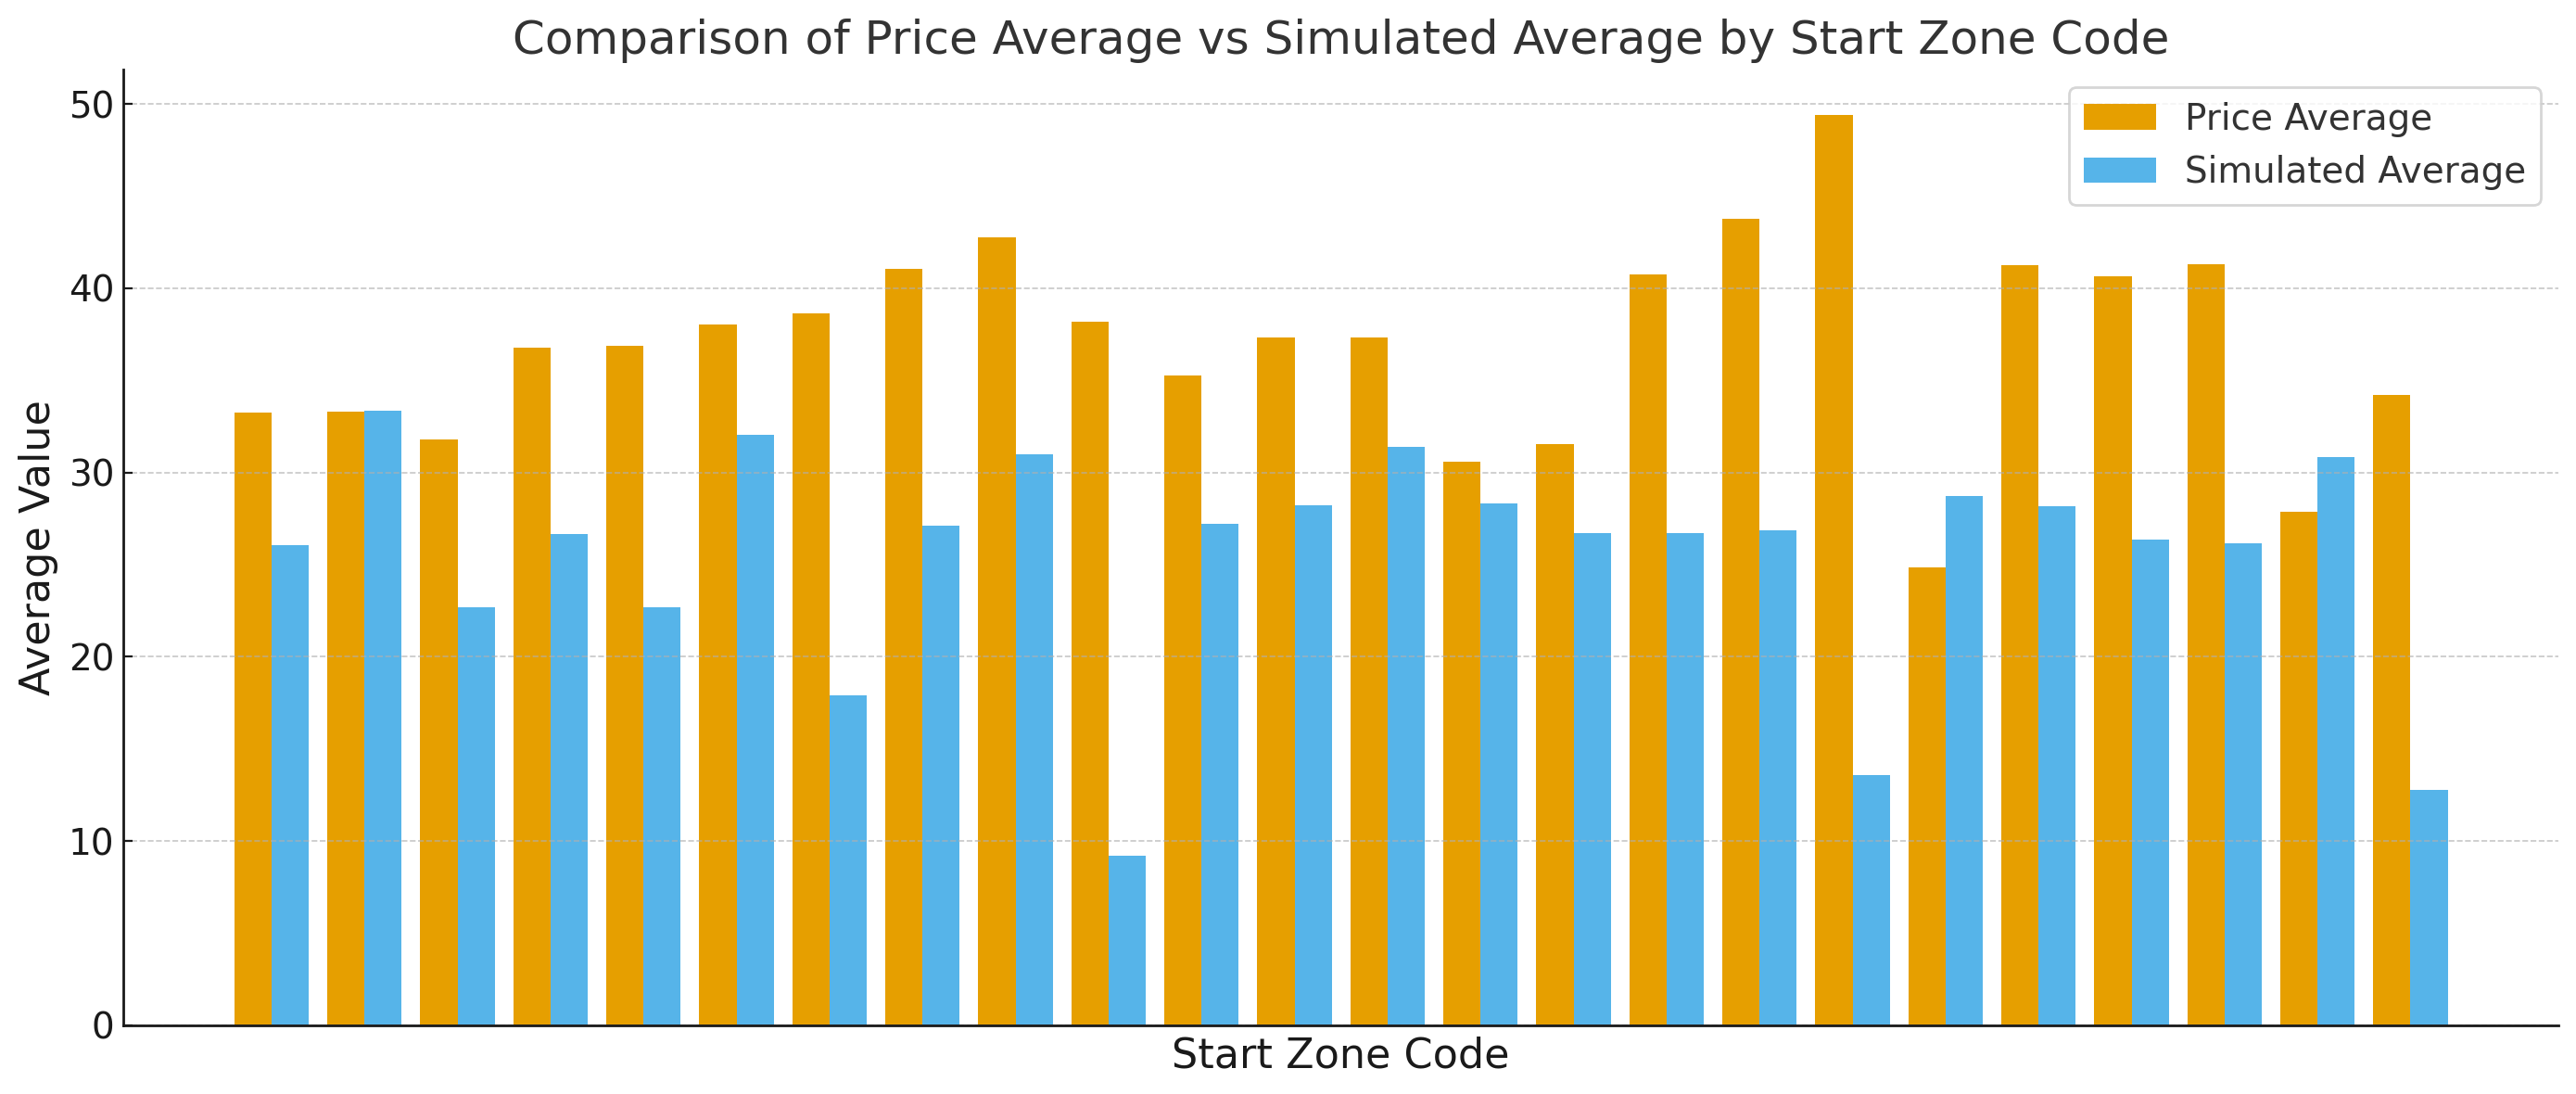
\includegraphics[width=0.5\linewidth]{images/PriceVsSimulatedPrice.png}
    \caption{Model Fit for the Short-run.}
    \label{fig:ModelFit}
\end{figure}

\begin{figure}
    \centering
    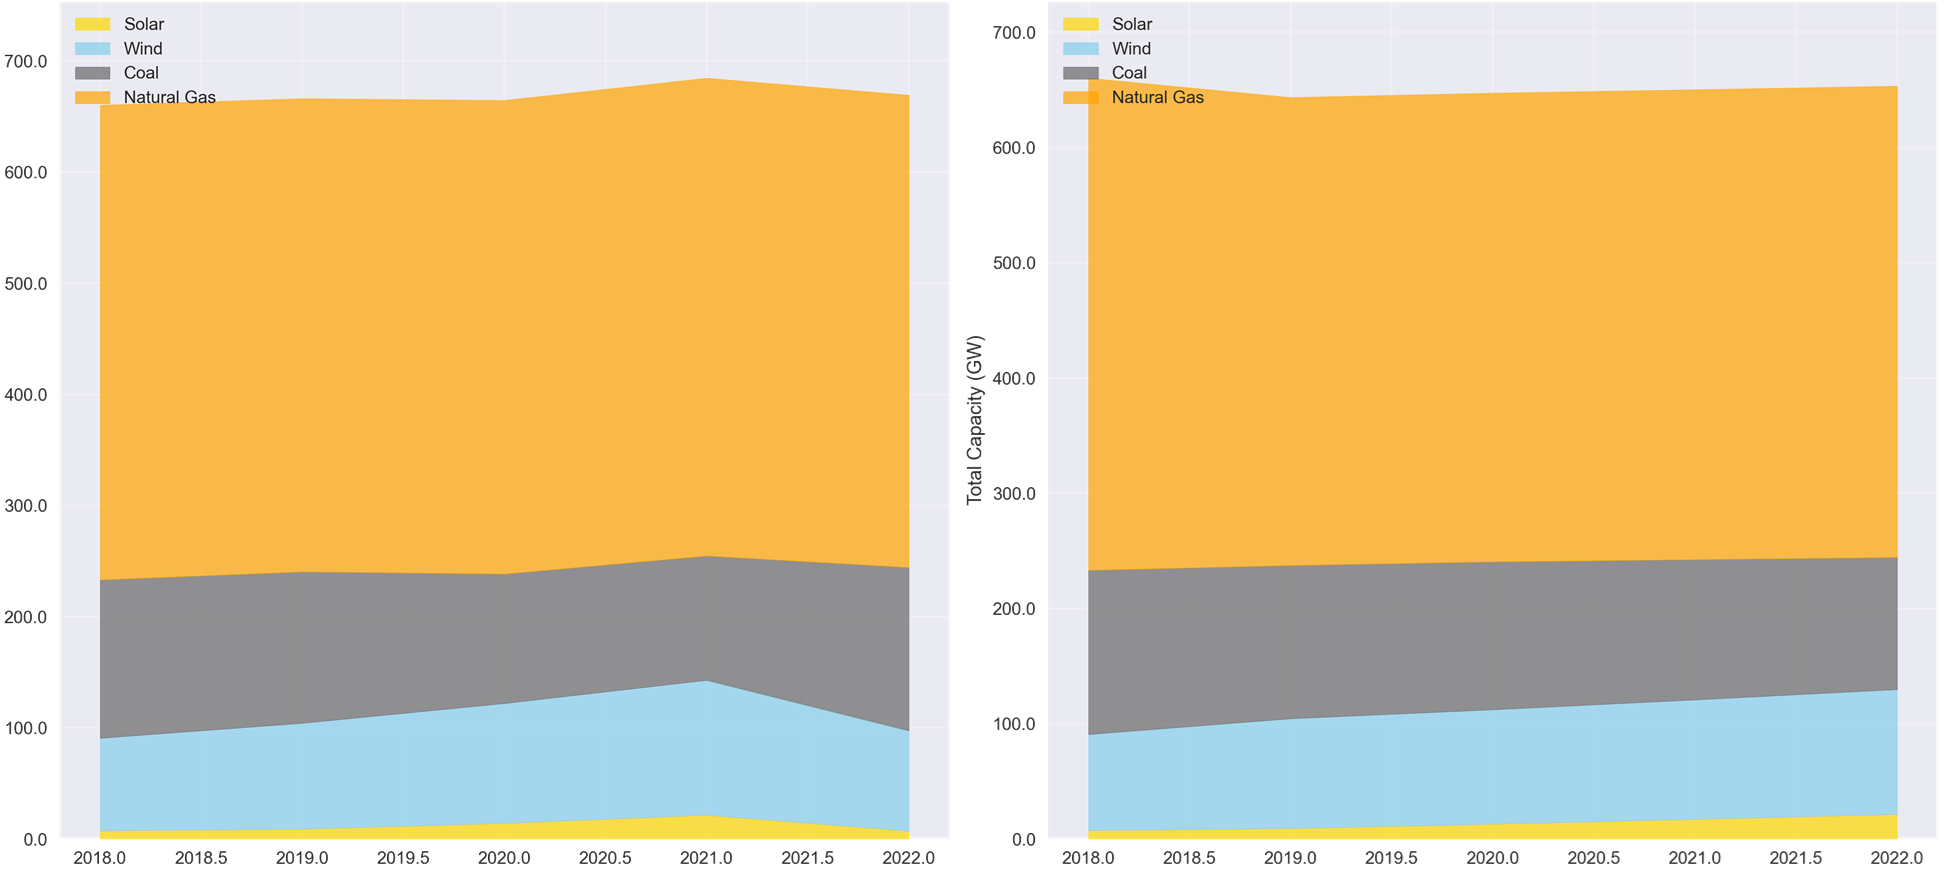
\includegraphics[width=0.5\linewidth]{images/capacity_stacked_area_Baseline.png}
    \caption{Model Fit for the Long-run.}
    \label{fig:longrunModelFit}
\end{figure}

\subsection{Robustness Checks}

I perform a suite of robustness checks detailed in Appendix Section \ref{app:robustness} and summarized in Table \ref{tab:robustness_summary}. I show the sensitivity of my a relaxation of assumptions. In particular, I show the robustness of my estimates to the allowance of blackouts and market power, varying assumptions about demand and its structure, changes to the specific dataset structure, and changes to other specific model features. The evidence presented is relatively compelling that the results are robust under slight relaxation. Some changes like market power have more impact on the estimated impacts as the level of deviation from the baseline assumption rises.

\section{Counterfactuals} \label{sec:Counterfactuals}

I use the estimated model to evaluate three sets of policy counterfactuals: upgrades to existing transmission infrastructure, addition of new long-distance transmission lines, and active federal legislation affecting both transmission and generation investment. In all counterfactual exercises, I hold estimated parameters fixed and modify only the primitives of the model---entry costs, line capacities, and per-MWh revenue---during simulation. This ensures that behavioral responses (investment, retirement, and dispatch) emerge endogenously from the estimated model rather than from re-fitting. The full set of counterfactuals run is described in Table \ref{tab:counterfactualRuns} and Figure \ref{fig:CounterfactualSimulations}.

\subsection{Transmission Infrastructure Upgrades}

The first set of counterfactuals examines the effects of upgrading existing transmission lines to High-Voltage Direct Current (HVDC) technology, which reduces line losses and increases transfer capacity. I simulate outcomes under full replacement of all inter-zonal lines as well as partial replacement of randomly selected lines at varying intensities.

Table \ref{tab:upgradeResults} reports the price impacts of transmission upgrades. Full replacement of all lines with HVDC technology reduces average wholesale prices by 6\% across the study region, generating welfare gains of approximately \$4 billion per year. This figure represents roughly one-third of total congestion costs estimated by Grid Strategies for the region. Notably, most of these gains can be achieved with partial upgrades: replacing 50\% of transmission lines still delivers price reductions exceeding 5\%.

Figure \ref{priceDecrease} illustrates how price reductions scale with the percentage of lines upgraded. The relationship exhibits diminishing returns, with the marginal benefit of additional upgrades declining as congestion on the most constrained corridors is relieved.

The effects of transmission upgrades vary substantially by region. The Northeast, where congestion costs are highest and renewable resources are scarce, experiences the largest price declines. The Midwest---home to abundant wind resources that are often curtailed due to transmission constraints---sees modest price increases as expanded export capacity raises local prices toward the national average. This price convergence, while increasing costs for some Midwestern consumers, reflects more efficient allocation of generation resources and reduced curtailment of low-cost renewable energy.

\begin{figure}
    \centering
    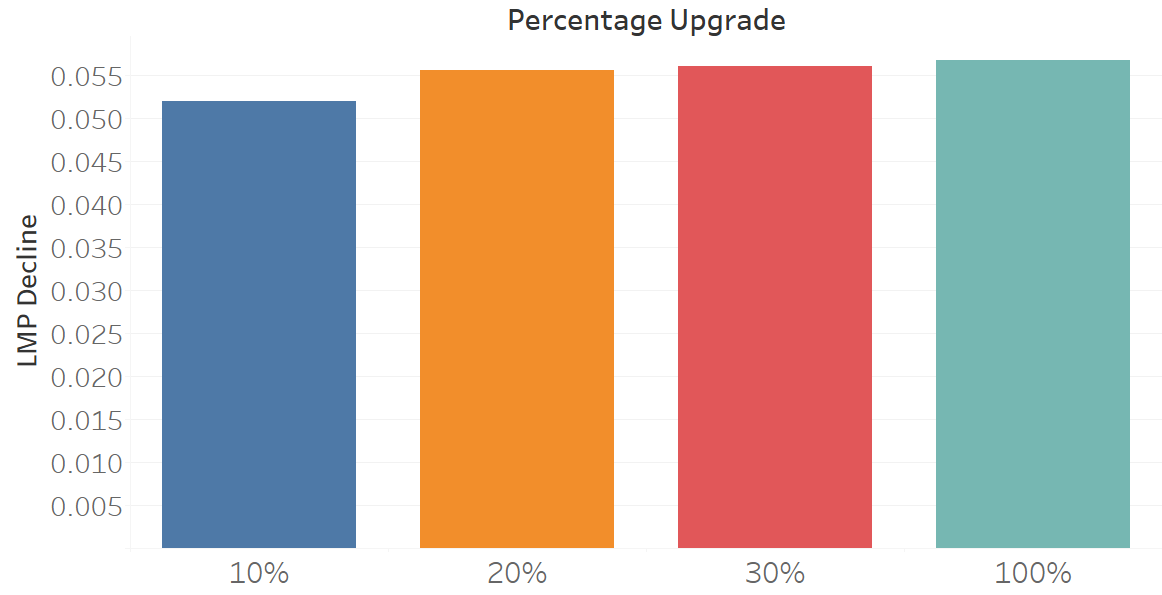
\includegraphics[width=1\linewidth]{images/LMP Decline by Percentage Upgrade.png}
    \caption{Price Decrease by Percentage Grid Upgrade}
    \label{priceDecrease}
\end{figure}

\subsection{New Long-Distance Transmission}

The second set of counterfactuals examines the addition of specific long-distance transmission projects. I first consider the limiting case of removing all transmission constraints, then evaluate specific proposed lines.

\subsubsection{Removal of All Transmission Constraints}

Eliminating all transmission constraints reduces average prices in every ISO except SPP and MISO, where prices increase as these regions become net exporters. This counterfactual also dramatically accelerates the renewable energy transition in the long-run model, as generators in renewables-rich regions can access distant markets without congestion-related price discounts.

%[PLACEHOLDER: Add specific price changes by ISO and renewable adoption numbers]

\subsubsection{Grain Belt Express}

The Grain Belt Express is a proposed 800-mile HVDC transmission line designed to carry 5,000 MW of wind power from western Kansas to Indiana and points east. In the long-run counterfactual, adding this line increases solar and wind adoption in the Eastern Interconnection by over 10\% by 2050, with the largest increases concentrated in SPP and western MISO where the line originates. 

%[PLACEHOLDER: Add additional results on prices and welfare]

\subsubsection{ERCOT-Eastern Interconnection Connection}

A major HVDC connection between ERCOT and the Eastern Interconnection would allow Texas's abundant wind and solar resources to serve load in the Southeast and beyond. 

%[PLACEHOLDER: Add description and results for the ERCOT interconnection counterfactual]

\subsection{Federal Legislation}

The final set of counterfactuals evaluates three pieces of federal legislation affecting electricity markets. These counterfactuals and their relationships are described in Table \ref{tab:factorialDesign}. I implement these policies as \textit{policy wedges}---time-varying modifications to model primitives that activate at each policy's enactment date while holding all estimated parameters fixed. This approach isolates the causal effect of each policy from the underlying structural relationships estimated from pre-policy data. To ensure comparability across scenarios, I use identical random seeds and shock draws for all simulations, so that differences across scenarios reflect only the policy treatment and not sampling variation. I run four scenarios: (i) both policies as enacted, (ii) IRA only, (iii) BIL only, and (iv) neither policy (the baseline).

\subsubsection{Big Wires Act}

The BIG WIRES Act (S.2827, 118th Congress) would mandate that each FERC Order No.\ 1000 transmission planning region achieve a Minimum Interregional Transfer Capacity (MITC) equal to at least 30\% of its coincident peak electrical demand, or an increase of 15\% over current capacity, whichever is lower, by 2035 as decribed in \cite{hickenlooper2023s}. The legislation is motivated by the widening gap between planned interregional transmission builds and anticipated need documented in the DOE's \cite{DOENationalTransmissionNeedsStudy}, driven by barriers including insufficient coordination across planning regions, cost allocation disputes, and local opposition \cite{joskow2021facilitating, pfeifenberger2021transmission}.

I follow the modeling approach of \cite{botterud2024evaluating}, who evaluate the BIG WIRES Act using the GenX capacity expansion model across 64 zones aggregated into 12 model regions that approximate the FERC Order No.\ 1000 planning regions. Their framework distinguishes interregional transmission (built between zones in different planning regions) from intraregional transmission (built within a region), and assumes that absent the Act, no new interregional transmission is built---reflecting the observed tendency of Balancing Authorities to prioritize investment within their own planning region. Under the Act, interregional capacity is expanded until each region satisfies the MITC requirement, with GenX determining the least-cost allocation of new capacity across corridors.

To implement this counterfactual in my model, I add inter-zonal transfer capacity consistent with the corridor-level builds reported in \cite{botterud2024evaluating}. I model the MITC requirement as time-varying capacity additions that phase in via a ramp function:
\begin{equation}
    A_{ij,t}^{\text{MITC}} = A_{ij,t}^{\text{baseline}} + \Delta A^{\text{MITC}}_{ij} \cdot \rho(t; t_0^{\text{MITC}}, R)
\end{equation}
where $\Delta A^{\text{MITC}}_{ij}$ is the additional transfer capacity on corridor $(i,j)$ required to satisfy the MITC constraint, calibrated to be consistent with the corridor-level estimates in \cite{botterud2024evaluating}. The largest capacity additions are concentrated in the Eastern Interconnection: between the Midwest and Mid-Atlantic, Southeast and Florida, Mid-Atlantic and Carolinas, Midwest and Central, and Mid-Atlantic and Southeast, which together account for approximately 80\% of total new interregional transmission builds under the Act.

%[PLACEHOLDER: Add specific corridor-level capacity additions used in model, mapping from Botterud et al. Table 1 to model zones, and results for prices, investment, emissions, and reliability]

\subsubsection{Inflation Reduction Act}

The Inflation Reduction Act (IRA) provides substantial tax credits for renewable energy investment, effectively reducing entry costs for solar and wind generators. I model the IRA through two channels that enter the simulation as policy wedges on the estimated model's primitives.

First, the IRA reduces entry costs for eligible renewable technologies. I implement this as a proportional reduction in the entry cost $E_k$ for eligible technology $k$:
\begin{equation}
    E_{k,t}^{\text{IRA}} = E_{k,t}^{\text{baseline}} \cdot (1 - \tau^{\text{IRA}}_k \cdot \rho(t; t_0, R))
\end{equation}
where $\tau^{\text{IRA}}_k \in [0,1)$ is the technology-specific cost reduction implied by the investment tax credit, $t_0$ is the IRA enactment date (August 2022, implemented as the first full period on or after enactment), and $\rho(t; t_0, R)$ is a ramp function that phases the credit in over $R$ periods to avoid discontinuities in the investment decision. I set $R$ to one year as a conservative default.

Second, the IRA production tax credit provides an ongoing per-MWh subsidy to eligible generators, which I model as a revenue shifter:
\begin{equation}
    P_{k,t}^{\text{eff}} = P_t + s^{\text{IRA}}_k \cdot \rho(t; t_0, R)
\end{equation}
where $s^{\text{IRA}}_k \geq 0$ is the production credit value in the same per-MWh units as the model's prices. This enters the generator's per-period profit function, raising effective revenue for eligible resources without altering the ISO's dispatch problem or the structure of the Bellman equation. Retirement decisions respond endogenously to the changed profit environment.

Eligibility is determined by a mapping from technology type to IRA-eligible status. In the baseline implementation, eligibility depends on technology $k$ alone and does not vary by region, though the framework accommodates region-specific eligibility if needed.

%[PLACEHOLDER: Add specific values of tau_IRA and s_IRA by technology, and results for renewable adoption, prices, and emissions]

\subsubsection{Bipartisan Infrastructure Law}

The Bipartisan Infrastructure Law (BIL) provides funding for transmission infrastructure including grants for interregional transmission projects. I model the BIL as a time-varying expansion of inter-zonal transfer capacities:
\begin{equation}
    A_{ij,t}^{\text{BIL}} = A_{ij,t}^{\text{baseline}} + \Delta A^{\text{BIL}}_{ij} \cdot \rho(t; t_0^{\text{BIL}}, R)
\end{equation}
where $\Delta A^{\text{BIL}}_{ij} \geq 0$ represents the additional transfer capacity on corridor $(i,j)$ funded by the BIL, in the same units as the baseline line limits $A_{ij}$, and $t_0^{\text{BIL}}$ is the BIL enactment date (November 2021). The adjusted capacities enter the ISO dispatch problem's constraint set, expanding the feasible region for inter-zonal power flows. The dispatch objective and optimality conditions are otherwise unchanged.

I consider two specifications for the BIL transmission expansion. The first is corridor-specific, assigning $\Delta A^{\text{BIL}}_{ij}$ values to individual lines consistent with announced project funding. The second is a system-wide specification in which each corridor receives a proportional expansion $\Delta A^{\text{BIL}}_{ij} = \alpha \cdot A_{ij,t}^{\text{baseline}}$, parameterized by a single scalar $\alpha > 0$.

%[PLACEHOLDER: Add specific corridor expansions or alpha value, and results]

\subsubsection{Combined Policy Effects}

Running these policies in combination reveals whether transmission investment and renewable subsidies act as substitutes or complements. Formally, I compare the welfare gain from the joint policy $\Delta W^{\text{IRA+BIL}} = W^{\text{as\_enacted}} - W^{\text{no\_ira\_no\_bil}}$ against the sum of individual effects $\Delta W^{\text{IRA}} + \Delta W^{\text{BIL}}$, where $\Delta W^{\text{IRA}} = W^{\text{no\_bil}} - W^{\text{no\_ira\_no\_bil}}$ and $\Delta W^{\text{BIL}} = W^{\text{no\_ira}} - W^{\text{no\_ira\_no\_bil}}$. Complementarity implies $\Delta W^{\text{IRA+BIL}} > \Delta W^{\text{IRA}} + \Delta W^{\text{BIL}}$.

The results indicate that these policies are largely complementary: renewable subsidies increase the supply of low-cost generation, while transmission investment ensures this generation can reach high-demand markets. The mechanism is intuitive---the IRA lowers entry costs, inducing additional renewable capacity in resource-rich regions, but the value of this capacity is limited by transmission constraints that prevent it from reaching high-price markets. The BIL relaxes these constraints, raising the effective price received by new entrants and amplifying the IRA's investment incentive. Implementing both policies together yields welfare gains exceeding the sum of individual effects, suggesting that a portfolio approach to energy transition policy dominates single-instrument strategies. I include estimates of the costs of the policies and show that all are welfare improving even after considering costs.

%[PLACEHOLDER: Add combined results with specific numbers]

\subsection{Welfare Decomposition}

I run a welfare decomposition where I demonstrate how gains accrue to producers and consumers at the zonal level. While the total system-wide surplus is obviously positive for both producers and consumers, the distribution of the surplus is significantly varied. In some regions, mainly ERCOT and specific zones within PJM, welfare is uniformly improved. This occurs because the insurance effect dominates with producers exporting more electricity during low-cost hours and importing during high-cost hours. For regions with significant renewable energy and low prices before transmission expansion, producer welfare increases while consumer welfare decreases. The opposite occurs in regions with fewer renewable resources and higher initial prices. I quantify these effects and provide useful intuition for policy-makers as to what transfers could be made to make the policy Pareto-improving.

\section{Conclusion} \label{sec:conclusion}

This paper develops and estimates a dynamic model of generator behavior in electricity markets with transmission constraints, linking short-run dispatch decisions to long-run capacity investment. The model captures how transmission infrastructure shapes price formation across interconnected markets and how these prices influence firms' incentives to invest in different generation technologies.

Three main findings emerge from the analysis. First, transmission constraints impose substantial costs on electricity consumers: upgrading existing infrastructure to modern HVDC standards would reduce wholesale prices by 6\% and generate \$4 billion in annual welfare gains. Second, the benefits of transmission investment are regionally heterogeneous, with the largest gains accruing to transmission-constrained regions in the Northeast. Third, in the long run, expanded transmission capacity accelerates the renewable energy transition by allowing generators in renewables-rich regions to access distant markets, increasing solar and wind adoption by over 10\% by 2050 under scenarios including major projects like the Grain Belt Express.

The policy counterfactuals indicate that transmission investment and renewable energy subsidies act as complements rather than substitutes. Policies like the Inflation Reduction Act increase the supply of renewable generation, while transmission investments under the Bipartisan Infrastructure Law and Big Wires Act ensure this generation can reach consumers. Implementing both types of policies together yields benefits exceeding the sum of their individual effects.

Several limitations suggest directions for future research. The model operates at the zonal rather than nodal level, preventing analysis of specific substation-to-substation connections. This limitation makes the model better suited to evaluating large-scale interregional transmission than individual line additions. Additionally, the model treats demand as exogenous; long-run shifts in the geographic distribution of load in response to electricity price changes represent an important extension. Finally, the model does not incorporate storage, which may interact with transmission as alternative solutions to renewable intermittency.

Despite these limitations, the results provide evidence that transmission investment offers a cost-effective complement to direct renewable subsidies in accelerating the energy transition. As policymakers evaluate proposals to expand interregional transmission capacity, models that capture both the short-run operational benefits and long-run investment effects can inform the efficient allocation of infrastructure spending.

\pagebreak

\singlespacing
\setlength\bibsep{0pt}
\printbibliography




\clearpage

\onehalfspacing

\section*{Tables} \label{sec:tab}
\addcontentsline{toc}{section}{Tables}

\begin{table}[htbp]
\centering
\begin{tabular}{lcccc}
\toprule
\textbf{ISO} & \textbf{Mean Price} & \textbf{Mean Load} & \textbf{Median Price} & \textbf{Median Load} \\
\midrule
ISO-NE & 50 & 13{,}623 & 45 & 13{,}308 \\
%IESO   & 20 & 16{,}140 & 11 & 15{,}283 \\
NYISO  & 43 & 17{,}686 & 39 & 17{,}297 \\
ERCOT  & 40 & 44{,}328 & 23 & 41{,}901 \\
%CAISO  & 46 & 25{,}477 & 39 & 24{,}585 \\
SPP    & 37 & 30{,}420 & 30 & 29{,}246 \\
MISO   & 38 & 73{,}945 & 34 & 72{,}179 \\
PJM    & 41 & 146{,}112 & 37 & 88{,}236 \\
\bottomrule
\end{tabular}
\caption{Average and Median Price and Load by ISO}
\label{priceData}
\end{table}

\begin{table}[htbp]
\centering
\begin{tabular}{lccc}
\toprule
\textbf{Variable} & \textbf{Mean} & \textbf{Standard Deviation} & \textbf{Median} \\
\midrule
Load & 5{,}075 & 7{,}055 & 2{,}296 \\
Price & 37.8 & 79.5 & 27.6 \\
SO\textsubscript{2} Emissions & 526 & 417 & 470 \\
Solar Generation & 2 & 13 & 0.03 \\
Wind Generation & 44 & 61 & 20 \\
Natural Gas Generation & 29 & 66 & 33 \\
Coal Generation & 162 & 217 & 64 \\
Exports & 18.9 & 76.3 & 0.53 \\
\bottomrule
\end{tabular}
\caption{Descriptive Statistics: Short-run}
\label{ShortTermStats1}
\end{table}

\begin{table}[htbp]
\centering
\begin{tabular}{lccc}
\toprule
\textbf{Variable} & \textbf{Mean} & \textbf{Standard Deviation} & \textbf{Median} \\
\midrule
Fuel Cost & 603 & 2{,}093 & 324 \\
Heat Content & 3.6 & 6.0 & 1.03 \\
Natural Gas Spot Price & 3.8 & 2.3 & 2.7 \\
%Natural Gas Futures Price & 3.8 & 2.1 & 2.7 \\
Coal Spot Price & 166 & 128 & 98 \\
Temperature & 13 & 12 & 15 \\
Loss Percentage & 0.05 & 0.06 & 0.05 \\
Transmission Constraint & 0.51 & 1.00 & 0.50 \\
Capacity Constraint & 0.06 & 66 & 33 \\
\bottomrule
\end{tabular}
\caption{Descriptive Statistics: Short-run}
\label{ShortTermStats2}
\end{table}

\begin{table}[htbp]
\centering
\begin{tabular}{lcccc}
\toprule
\textbf{Resource} & \textbf{Intercept} & \textbf{Signif.} & \textbf{Export Coeff.} & \textbf{Signif.} \\
\midrule
Electricity used for energy storage & 30.97 & *** & 0.02 & *** \\
Natural Gas                         & 37.72& *** & 0.01 &  ***\\
Nuclear (incl. Uranium, Plutonium, Thorium) & 46.44 & *** & 0.01 & *** \\
Coal                                & 30.97 & *** & 32.47 & *** \\
Distillate Fuel Oil (diesel, No.\,1--4) & 33.23 &  *** & 0.01 & *** \\
Landfill Gas                        & 33.91 & *** & 0.00 & *** \\
Water at hydro or hydrokinetic technologies & 36.27 & *** & -0.02 & *** \\
Other Biomass Gas (digester, methane, etc.) & 27.64 & *** & -0.11 & *** \\
Petroleum Coke                      & 31.50 & *** & 0.06 &  ***\\
Wood/Wood Waste Solids              & 40.91 &  ***& 0.06 &  ***\\
Blast Furnace Gas                   & 30.34 & *** & 0.00 &  ***\\
Waste heat (no direct fuel source) & 37.43 & *** & 0.01 &  ***\\
Black Liquor                        & 30.97 & *** & 0.01 & *** \\
Other Gas                           & 41.99 & *** & -0.12 & *** \\
Other                               & 30.97 & *** & 0.10 & *** \\
Purchased Steam                     & 30.97 & *** & -0.02 & *** \\
Agricultural By-Products            & 29.56 & *** & -0.06 &  ***\\
Petroleum Products                  & 34.94 & *** & 0.00 & *** \\
\bottomrule
\end{tabular}
\vspace{0.5em}

\footnotesize\textit{Note:} Export coefficients represent the marginal relationship between exports and output by energy resource. Significance codes: *** $p<0.01$, ** $p<0.05$, * $p<0.1$. The log-likelihood of the regression is 7.662301.
\caption{Short-run Model Estimates by Resource Type}
\label{ResourcesTable}
\end{table}

\begin{table}[htbp]
\centering
\begin{tabular}{lcc}
\toprule
\textbf{Variable} & \textbf{Estimate} & \textbf{Significance} \\
\midrule
Natural Gas Price & 6.93 & *** \\
Dewpoint               & 2.46 & *** \\
Temperature            & 0.00 &     \\
Heat Content              & -2.22& *** \\
Generator Startup              & -2.3& *** \\
 Generator Near Capacity             & -2.3& *** \\
\bottomrule
\end{tabular}
\vspace{0.5em}

\footnotesize\textit{Notes:} Specification includes hourly and monthly dummies, zone-code dummies, and severe weather dummies.
\caption{Estimates for Natural Gas Covariates}
\label{NaturalGasTable}
\end{table}

\begin{table}[htbp]
\centering
\begin{tabular}{lcc}
\toprule
\textbf{Variable} & \textbf{Estimate} & \textbf{Significance} \\
\midrule
Coal Price     & 8.68  & *** \\
Dewpoint       & 2.46  & *** \\
Temperature    & 4.00  & *** \\
Heat Rate      & -1.30 & *** \\
Generator Startup              & -2.3& *** \\
 Generator Near Capacity             & -2.3& *** \\
\bottomrule
\end{tabular}
\vspace{0.5em}

\footnotesize\textit{Notes:} Specification includes hourly and monthly dummies, zone-code dummies, and severe weather dummies.
\caption{Estimates for Coal Covariates}
\label{CoalTable}
\end{table}

% ============================================================
% Table 1: Master table of all counterfactual runs
% ============================================================

\begin{landscape}
    \begin{table}[htbp]
        \centering
        \caption{Counterfactual Simulation Scenarios}
        \label{tab:counterfactualRuns}
        \small 
        % Defines columns: 
        % 1: Left align (Scenario)
        % 2: Paragraph 5cm (Description)
        % 3-5: Centered paragraph 2.5cm (The checkmark columns)
        \begin{tabular}{@{} l p{5cm} >{\centering\arraybackslash}p{2.5cm} >{\centering\arraybackslash}p{2.5cm} >{\centering\arraybackslash}p{2.5cm} @{}}
            \toprule
            & & \multicolumn{3}{c}{\textit{Modified Primitives}} \\
            \cmidrule(lr){3-5}
            \textbf{Scenario} & \textbf{Description} & Line Capacity \newline $A_{ij}$ & Entry Cost \newline $E_k$ & Revenue \newline $P_k^{\text{eff}}$ \\
            \midrule
            
            % --- PANEL A ---
            \multicolumn{5}{l}{\textit{Panel A: Transmission Infrastructure Upgrades}} \\[0.5ex]
            Full HVDC & All inter-zonal lines replaced with HVDC & $\checkmark$ & & \\
            Partial HVDC & Random subset at intensity $\alpha \in (0,1)$ & $\checkmark$ & & \\[1.5ex]
            
            % --- PANEL B ---
            \multicolumn{5}{l}{\textit{Panel B: New Long-Distance Transmission}} \\[0.5ex]
            No constraints & All transmission limits removed & $\checkmark$ & & \\
            Grain Belt Express & 5,000~MW HVDC, KS to IN & $\checkmark$ & & \\
            ERCOT--Eastern IC & HVDC link, ERCOT to Southeast & $\checkmark$ & & \\[1.5ex]
            
            % --- PANEL C ---
            \multicolumn{5}{l}{\textit{Panel C: Federal Legislation}} \\[0.5ex]
            BIG WIRES Act & MITC $\geq$ 30\% peak demand by 2035 & $\checkmark$ & & \\[1.5ex]
            
            \multicolumn{5}{l}{\quad\textit{IRA $\times$ BIL Factorial Design}} \\[0.5ex]
            Baseline & Neither IRA nor BIL & & & \\
            IRA only & IRA enacted, no BIL & & $\checkmark$ & $\checkmark$ \\
            BIL only & BIL enacted, no IRA & $\checkmark$ & & \\
            As enacted & Both IRA and BIL & $\checkmark$ & $\checkmark$ & $\checkmark$ \\[1.5ex]
            
            % --- PANEL D ---
            \multicolumn{5}{l}{\textit{Panel D: Cross-Cutting Analysis}} \\[0.5ex]
            Welfare & Producer/consumer surplus & \multicolumn{3}{c}{\textit{Applied to all scenarios}} \\
            decomposition & by zone for each scenario & \multicolumn{3}{c}{} \\
            \bottomrule
        \end{tabular}
        
        % Table Notes (Placed simply below the tabular)
        \vspace{1ex}
        \begin{minipage}{\linewidth}
            \footnotesize
            \textit{Notes:} Each scenario holds estimated structural parameters fixed and modifies only the indicated model primitives. $A_{ij}$ denotes inter-zonal transfer capacity, $E_k$ denotes technology-specific entry cost, and $P_k^{\text{eff}}$ denotes effective per-MWh revenue inclusive of production tax credits. All policy wedges phase in via a ramp function $\rho(t; t_0, R)$ to avoid discontinuities. Panel~C scenarios use identical random seeds and shock draws to isolate policy effects from sampling variation.
        \end{minipage}
    \end{table}
\end{landscape}

%\vspace{1.5cm}

% ============================================================
% Table 2: Federal legislation factorial design and
%          complementarity comparisons
% ============================================================

\begin{table}[htbp]
\centering
\begin{threeparttable}
\caption{Federal Legislation: Factorial Design and Complementarity Test}
\label{tab:factorialDesign}
\small
\begin{tabular}{@{} l cc @{}}
\toprule
& \multicolumn{2}{c}{\textbf{Bipartisan Infrastructure Law}} \\
\cmidrule(lr){2-3}
\textbf{Inflation Reduction Act} & Not enacted & Enacted \\
\midrule
Not enacted & $W^{\text{baseline}}$ & $W^{\text{BIL only}}$ \\[10pt]
Enacted & $W^{\text{IRA only}}$ & $W^{\text{as enacted}}$ \\
\bottomrule
\end{tabular}

\vspace{0.6cm}

\begin{tabular}{@{} L{4.2cm} l @{}}
\toprule
\textbf{Comparison} & \textbf{Definition} \\
\midrule
IRA marginal effect & $\Delta W^{\text{IRA}} = W^{\text{IRA only}} - W^{\text{baseline}}$ \\[4pt]
BIL marginal effect & $\Delta W^{\text{BIL}} = W^{\text{BIL only}} - W^{\text{baseline}}$ \\[4pt]
Joint effect & $\Delta W^{\text{joint}} = W^{\text{as enacted}} - W^{\text{baseline}}$ \\[4pt]
Complementarity & $\Delta W^{\text{joint}} - \bigl(\Delta W^{\text{IRA}} + \Delta W^{\text{BIL}}\bigr) > 0$ \\
\bottomrule
\end{tabular}

\begin{tablenotes}[flushleft]
\footnotesize
\item \textit{Notes:} $W$ denotes total welfare (consumer plus producer surplus). The top panel displays the $2 \times 2$ factorial structure of the federal legislation counterfactuals. The bottom panel defines the comparisons used to test policy complementarity. Complementarity holds when the joint welfare gain exceeds the sum of individual gains, indicating that transmission investment (BIL) and renewable subsidies (IRA) are mutually reinforcing.
\end{tablenotes}
\end{threeparttable}
\end{table}

% \begin{table}[ht]
% \centering
% \caption{Resource-Specific Parameter Estimates}
% \begin{threeparttable}
% \resizebox{\textwidth}{!}{%
% \begin{tabular}{l*{8}{c}}
% \toprule
% \textbf{Resource Type} & $F_0$ & $E_0$ & $\rho_{1k}$ & $\rho_{2k}$ & $\psi_{1k}$ & $\sigma^2_{\zeta_1}$ & $\sigma^2_{\zeta_2}$ & $\psi_{2k}$ \\
%  & (s.e.) & (s.e.) & (s.e.) & (s.e.) & (s.e.) & (s.e.) & (s.e.) & (s.e.) \\
% \midrule
% Coal         & -0.080 &  0.160 & -0.151 &  0.019 & -0.015 & 0.127 &  0.055 & -0.106 \\
%              & [PLACEHOLDER] & [PLACEHOLDER] & [PLACEHOLDER] & [PLACEHOLDER] & [PLACEHOLDER] & [PLACEHOLDER] & [PLACEHOLDER] & [PLACEHOLDER] \\
% Natural Gas  & -0.242 & -0.116 & -0.076 &  0.058 &  0.140 & 0.155 &  0.172 &  0.128 \\
%              & [PLACEHOLDER] & [PLACEHOLDER] & [PLACEHOLDER] & [PLACEHOLDER] & [PLACEHOLDER] & [PLACEHOLDER] & [PLACEHOLDER] & [PLACEHOLDER] \\
% Solar        &  0.091 &  0.018 & -0.115 &  0.072 &  0.102 & 0.048 & 0.085 &  0.017 \\
%              & [PLACEHOLDER] & [PLACEHOLDER] & [PLACEHOLDER] & [PLACEHOLDER] & [PLACEHOLDER] & [PLACEHOLDER] & [PLACEHOLDER] & [PLACEHOLDER] \\
% Wind         &  0.276 & -0.007 & -0.081 &  0.223 & -0.191 & 0.027 & 0.142 &  0.095 \\
%              & [PLACEHOLDER] & [PLACEHOLDER] & [PLACEHOLDER] & [PLACEHOLDER] & [PLACEHOLDER] & [PLACEHOLDER] & [PLACEHOLDER] & [PLACEHOLDER] \\
% \bottomrule
% \end{tabular}
% }
% \begin{tablenotes}
% \small
% \item \textit{Notes:} Standard errors in brackets. [PLACEHOLDER: Add note on estimation method for standard errors]
% \end{tablenotes}
% \end{threeparttable}
% \label{longRunResults}
% \end{table}

% \begin{table}[htbp]
% \centering
% \caption{Price Impacts of Transmission Upgrades}
% \begin{tabular}{lcccc}
% \toprule
% \textbf{Upgrade Percentage} & \textbf{Avg. Price Change} & \textbf{Welfare Gain (\$/yr)} & \textbf{NE Change} & \textbf{MW Change} \\
% \midrule
% 25\% & [PLACEHOLDER] & [PLACEHOLDER] & [PLACEHOLDER] & [PLACEHOLDER] \\
% 50\% & $>$5\% reduction & [PLACEHOLDER] & [PLACEHOLDER] & [PLACEHOLDER] \\
% 75\% & [PLACEHOLDER] & [PLACEHOLDER] & [PLACEHOLDER] & [PLACEHOLDER] \\
% 100\% & 6\% reduction & \$4 billion & Largest decline & Modest increase \\
% \bottomrule
% \end{tabular}
% \label{tab:upgradeResults}
% \end{table}

\clearpage

\section*{Figures} \label{sec:fig}
\addcontentsline{toc}{section}{Figures}

% \begin{center}
% \begin{figure}
% \begin{tikzpicture}[node distance=2cm, every node/.style={align=center, font=\small}, scale=.45, transform shape]

%     % Supply Nodes with Labels above the boxes
%     \node (supply1_label) [above=0.2cm] at (0,0) {Supply Node $j$};
%     \node (supply1) [draw, rectangle, minimum width=3cm, minimum height=5cm, below=0.2cm of supply1_label] {};

%     \node (supply2_label) [above=0.2cm, right=6cm of supply1_label] {Supply Node $j'$};
%     \node (supply2) [draw, rectangle, minimum width=3cm, minimum height=5cm, below=0.2cm of supply2_label] {};

%     % Generators at Supply Node j
%     \node (gen1) [draw, rectangle, below=0.8cm of supply1.north, minimum width=2.5cm] {Generator $G$};
%     \node (gen1_label) [left=0.5cm of gen1] {Marginal Resource};

%     \node (gen2) [draw, rectangle, below=0.8cm of gen1, minimum width=2.5cm] {Generator $G'$};
%     \node (gen2_label) [left=0.5cm of gen2] {Capacity Constrained};

%     % Generators at Supply Node j'
%     \node (gen3) [draw, rectangle, below=0.8cm of supply2.north, minimum width=2.5cm] {Generator $G$};
%     \node (gen3_label) [right=0.5cm of gen3] {Marginal Resource};

%     \node (gen4) [draw, rectangle, below=0.8cm of gen3, minimum width=2.5cm] {Generator $G'$};
%     \node (gen4_label) [right=0.5cm of gen4] {};

%     % Demand Nodes
%     \node (demand1) [draw, circle, minimum width=1cm, below=4cm of supply1, label=below:{Demand Node $i$}] {Demand Node $i$, $L_i,LMP_i$};
%     \node (demand2) [draw, circle, minimum width=1cm, below=4cm of supply2, label=below:{Demand Node $i'$}] {Demand Node $i'$, $L_i',LMP_i'$};

%     % Arrows from Supply Nodes to Demand Nodes with Labels
%     \draw[-{Stealth}, thick] (supply1.south) to [out=-135, in=135, looseness=1.5] (demand1.north) node[midway, left, xshift=-0.3cm] {};
%     \draw[-{Stealth}, thick, dashed] (supply1.south) to [out=-45, in=135, looseness=1.2] (demand2.north) node[midway, above, xshift=0.5cm] {};
%     \draw[-{Stealth}, thick, dashed] (supply2.south) to [out=-135, in=45, looseness=1.2] (demand1.north east) node[midway, right, xshift=-0.3cm] {};
%     \draw[-{Stealth}, thick] (supply2.south) to [out=-45, in=45, looseness=1.5] (demand2.north) node[midway, right, xshift=-0.3cm] {};

% \end{tikzpicture}
%     \caption{Sample two-node network.}
%     \label{SampleNetwork}
% \end{figure}
% \end{center}

\begin{center}
   \begin{figure}[H]
\begin{tikzpicture}[
    scale=0.72,
    transform shape,
    node distance=0.48cm and 0.7cm,
    % === STYLES ===
    source/.style={
        cylinder,
        shape border rotate=90,
        draw=#1!60!black,
        fill=#1!12,
        text centered,
        minimum height=1.55em,
        minimum width=1.6cm,
        aspect=0.35,
        font=\tiny,
        align=center
    },
    source/.default=green,
    process/.style={
        rectangle,
        draw=blue!50!black,
        fill=blue!10,
        text centered,
        rounded corners=2pt,
        minimum height=1.35em,
        minimum width=1.8cm,
        font=\tiny,
        align=center
    },
    dispatch/.style={
        rectangle,
        draw=orange!70!black,
        fill=orange!20,
        text centered,
        rounded corners=2pt,
        minimum height=1.6em,
        minimum width=1.9cm,
        font=\tiny\bfseries,
        align=center
    },
    model/.style={
        rectangle,
        draw=red!60!black,
        fill=red!12,
        thick,
        text centered,
        rounded corners=3pt,
        minimum height=1.85em,
        minimum width=2.2cm,
        font=\scriptsize\bfseries,
        align=center
    },
    arrow/.style={
        -{Stealth[scale=0.65]},
        semithick,
        color=gray!70!black
    },
    directarrow/.style={
        -{Stealth[scale=0.55]},
        color=blue!50!black,
        thin
    },
    grouplabel/.style={
        font=\tiny\bfseries,
        color=gray!70!black
    },
    annot/.style={
        font=\scriptsize,
        color=gray!60!black
    }
]

% === COLUMN 1: RAW DATA SOURCES ===

% Generator/Capacity Data (green shades)
\node[source=green!80!black] (eia860) {EIA 860};
\node[source=green!80!black, below=0.26cm of eia860] (eia923) {EIA 923};

% Real-time/Operational Data (teal shades)
\node[source=teal, below=0.35cm of eia923] (iso) {ISO Data};
\node[source=teal, below=0.26cm of iso] (campd) {EPA CAMPD};

% Grid Infrastructure (cyan shades)
\node[source=cyan!70!black, below=0.35cm of campd] (hifld) {HIFLD};
\node[source=cyan!70!black, below=0.26cm of hifld] (spiq) {S\&P Capital IQ};

% Flows and Weather (blue-green shades)
\node[source=blue!60!green, below=0.35cm of spiq] (eia930) {EIA 930};
\node[source=blue!60!green, below=0.26cm of eia930] (weather) {Meteostat};

% === COLUMN 2: DATA CONSTRUCTION STEPS ===

% Generation Estimation
\node[process, right=1.5cm of eia923, yshift=-0.1cm] (gen_est) {Estimate Hourly\\Gen.\ by Zone};

% Transmission Network
\node[process, right=1.5cm of hifld, yshift=-0.1cm] (trans_est) {Flow Limits \&\\Line Losses};

% Load Adjustment
\node[process, right=1.5cm of eia930] (load_adj) {Adjust Load for\\External BA};

% Dispatch Simulation (central step)
\node[dispatch, right=2.8cm of campd, yshift=-0.4cm] (dispatch) {Optimal Dispatch\\Simulation};

% === COLUMN 3: ESTIMATION MODELS ===

% Short-Run Model
\node[model, right=1.8cm of dispatch, yshift=0.7cm] (short_run) {Short-Run Model};

% Long-Run Model  
\node[model, below=0.8cm of short_run] (long_run) {Long-Run Model};

% Projection Sources (for Long-Run)
\node[source=purple, right=0.7cm of long_run, yshift=0.2cm] (aeo) {EIA AEO};
\node[source=purple, below=0.2cm of aeo] (nrel) {NREL};

% === CONNECTIONS ===

% To Generation Estimation
\draw[arrow] (eia860.east) -- ++(0.35,0) |- (gen_est.170);
\draw[arrow] (eia923.east) -- ++(0.35,0) |- (gen_est.west);
\draw[arrow] (iso.east) -- ++(0.4,0) |- (gen_est.190);
\draw[arrow] (campd.east) -- ++(0.45,0) |- (gen_est.210);

% To Transmission Estimation
\draw[arrow] (hifld.east) -- ++(0.35,0) |- (trans_est.170);
\draw[arrow] (spiq.east) -- ++(0.35,0) |- (trans_est.190);

% To Load Adjustment
\draw[arrow] (eia930) -- (load_adj);

% To Dispatch Simulation - arrows enter from top-left area to avoid text
\draw[arrow] (gen_est.east) -- ++(0.25,0) |- (dispatch.north west);
\draw[arrow] (trans_est.east) -- ++(0.15,0) |- (dispatch.west);
\draw[arrow] (load_adj.east) -- ++(0.2,0) |- (dispatch.south west);

% Dispatch to Short-Run Model
\draw[arrow] (dispatch.east) -- ++(0.25,0) |- node[pos=0.75, above, annot] {MC curves} (short_run.west);

% Direct feeds to Short-Run Model
\draw[directarrow] (weather.east) -- ++(4.5,0) |- (short_run.230);
\draw[directarrow] (iso.east) -- ++(4.8,0) |- (short_run.130);

% Short-Run to Long-Run
\draw[arrow] (short_run.south) -- node[midway, right, annot] {Rev.\ est.} (long_run.north);

% Projections to Long-Run
\draw[arrow] (aeo.west) -- (long_run.10);
\draw[arrow] (nrel.west) -- (long_run.350);

% EIA 860 capacity data to Long-Run
\draw[directarrow] (eia860.east) -- ++(6.55,0) |- (long_run.130);

% === BACKGROUND GROUPINGS ===
\begin{scope}[on background layer]
    % Raw Data Sources
    \node[fit=(eia860)(weather), 
          fill=gray!7, 
          rounded corners=3pt, 
          draw=gray!30,
          inner sep=4pt] (rawbox) {};
    \node[grouplabel, above=0.02cm of rawbox.north] {Data Sources (2018--2023)};
    
    % Data Construction
    \node[fit=(gen_est)(load_adj)(dispatch)(trans_est), 
          fill=blue!5, 
          rounded corners=3pt, 
          draw=blue!20,
          inner sep=5pt] (constructbox) {};
    \node[grouplabel, above=0.02cm of constructbox.north] {Dataset Construction};
    
    % Models
    \node[fit=(short_run)(long_run), 
          fill=red!5, 
          rounded corners=3pt, 
          draw=red!20,
          inner sep=5pt] (modelbox) {};
    \node[grouplabel, above=0.02cm of modelbox.north] {Estimation};
    
    % Projections
    \node[fit=(aeo)(nrel), 
          fill=purple!8, 
          rounded corners=2pt, 
          draw=purple!25,
          inner sep=3pt] (projbox) {};
    \node[grouplabel, below=0.01cm of projbox.south, color=purple!60!black] {Projections (to 2050)};
\end{scope}

% === ANNOTATIONS ===
% Position LMP annotation below dispatch box, slightly right of center to avoid arrows
\node[annot, below=0.1cm of dispatch.south, xshift=0.9cm] {Low $\to$ High LMP};

% ISO coverage note
\node[font=\fontsize{4}{5}\selectfont, color=gray!50!black, below=0.12cm of rawbox.south, text width=2.2cm, align=center] 
    {ISOs: SPP, MISO, PJM,\\NYISO, ISO-NE, ERCOT};

\end{tikzpicture}
    \caption{Dataset Construction Diagram.}
    \label{DataSetCreation}
    \end{figure}
\end{center}

% \begin{center}
%    \begin{figure}
%     \begin{tikzpicture}[scale=0.225, every node/.style={transform shape},
%         block/.style={rectangle, draw, text centered, rounded corners, minimum height=2.5em, minimum width=11em, fill=blue!10, font=\Huge},
%         arrow/.style={-{Stealth[scale=1]}, thick},
%         node distance=3cm  % Increase node distance for more space
%     ]
%         % Input Sources
%         \node[block] (iso) {ISO Data \\ (Load, Price, Fuel Mix)};
%         \node[block, below=of iso, yshift=-0.5cm] (net_exports) {Net Exports \\ (EIA)};

%         % Generation Data and Generator Data
%         \node[block, right=6cm of iso] (generation) {Generation Data};
%         \node[block, above=of generation, yshift=0.5cm] (generator) {Generator Data \\ (EIA 923, EPA CAMPD, EIA 860)};

%         % Processes
%         \node[block, below=3.5cm of generation] (line_loss) {Estimate Line Losses \& Flow Limits};
%         \node[block, below=of line_loss, yshift=-0.5cm] (load_adjust) {Adjust Load by Net Exports};

%         % Export Estimation and Final Estimation
%         \node[block, below=of load_adjust, yshift=-0.5cm] (exports) {Export Approximation Process};
%         \node[block, right=4cm of exports] (estimation) {Short-run Estimation (ML)};
        
%         % Long-Run Estimation and Inputs
%         \node[block, below=of estimation, yshift=-0.5cm] (long_run) {Long-Run Estimation (Dynamic model with GMM)};
%         \node[block, below left=2cm and 1cm of long_run] (past_data) {Past Data Capacity, \\ Weather, Prices \\ (EIA, Prism, S\&P)};
%         \node[block, below right=2cm and 1cm of long_run] (future_data) {Future Data \\ (EIA Outlook)};
        
%         % Additional Input: Weather and Price Data
%         \node[block, above=of estimation, yshift=-0.5cm] (weather) {Weather and Price Data \\ (EIA, S\&P, Prism)};

%         % Move Transmission Lines to the right of line_loss
%         \node[block, right=6cm of line_loss] (transmission) {Transmission Lines \\ (Homeland Infrastructure, S\&P Capital IQ)};

%         % Adjusted Arrows
%         \draw[arrow] (iso.east) -- ++(1,0) |- (generation.west);  % ISO Data to Generation Data
%         \draw[arrow] (generator) -- (generation);  % Generator Data directly above Generation Data
%         \draw[arrow] (transmission.west) -- (line_loss.east);  % Transmission Lines to Estimate Line Losses
%         \draw[arrow] (generation) -- (line_loss);  % Generation Data to Estimate Line Losses
%         \draw[arrow] (net_exports.east) -| ++(1.5,0) |- (load_adjust.west);  % Net Exports to Adjust Load by Net Exports
%         \draw[arrow] (line_loss) -- (load_adjust);  % Line Losses to Adjust Load by Net Exports
%         \draw[arrow] (load_adjust) -- (exports);  % Adjust Load to Export Approximation Process
%         \draw[arrow] (exports) -- (estimation);  % Export Process to Short-run Estimation
%         \draw[arrow] (weather) -- (estimation);  % Weather and Price Data to Short-run Estimation
%         \draw[arrow] (estimation) -- (long_run);  % Short-run Estimation to Long-run Estimation
%         \draw[arrow] (past_data) -- (long_run);  % Past Data to Long-run Estimation
%         \draw[arrow] (future_data) -- (long_run);  % Future Data to Long-run Estimation

%     \end{tikzpicture}
%     \caption{Dataset Construction Diagram.}
%     \label{DataSetCreation}
%     \end{figure}
% \end{center}

\begin{figure}[H]
    \centering
    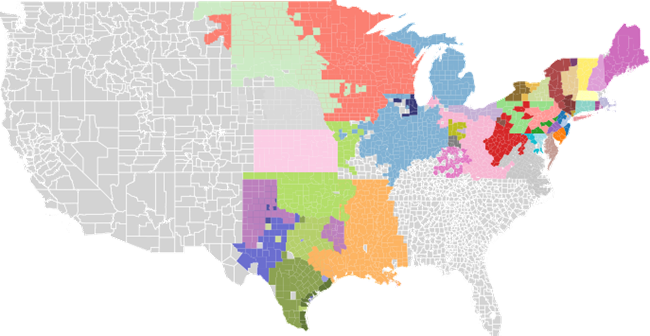
\includegraphics[width=0.5\linewidth]{images/ZoneMap (3).png}
    \caption{Mapped Zones from Market.}
    \label{fig:ZoneMap}
\end{figure}


\begin{figure}[H]
    \centering
    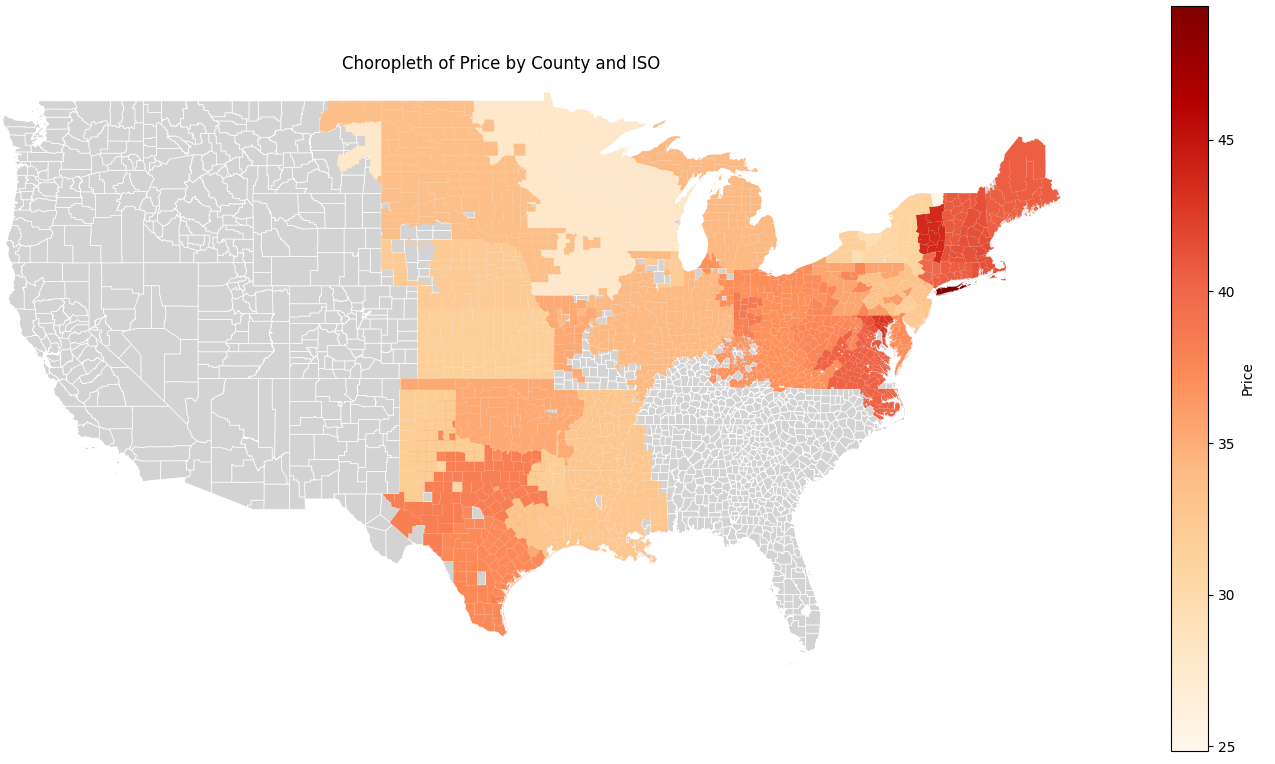
\includegraphics[width=0.5\linewidth]{images/PriceMap (2).png}
    \caption{Locational Marginal Price by Zone in Data.}
    \label{fig:PriceMap}
\end{figure}

\begin{figure}[H]
    \centering
    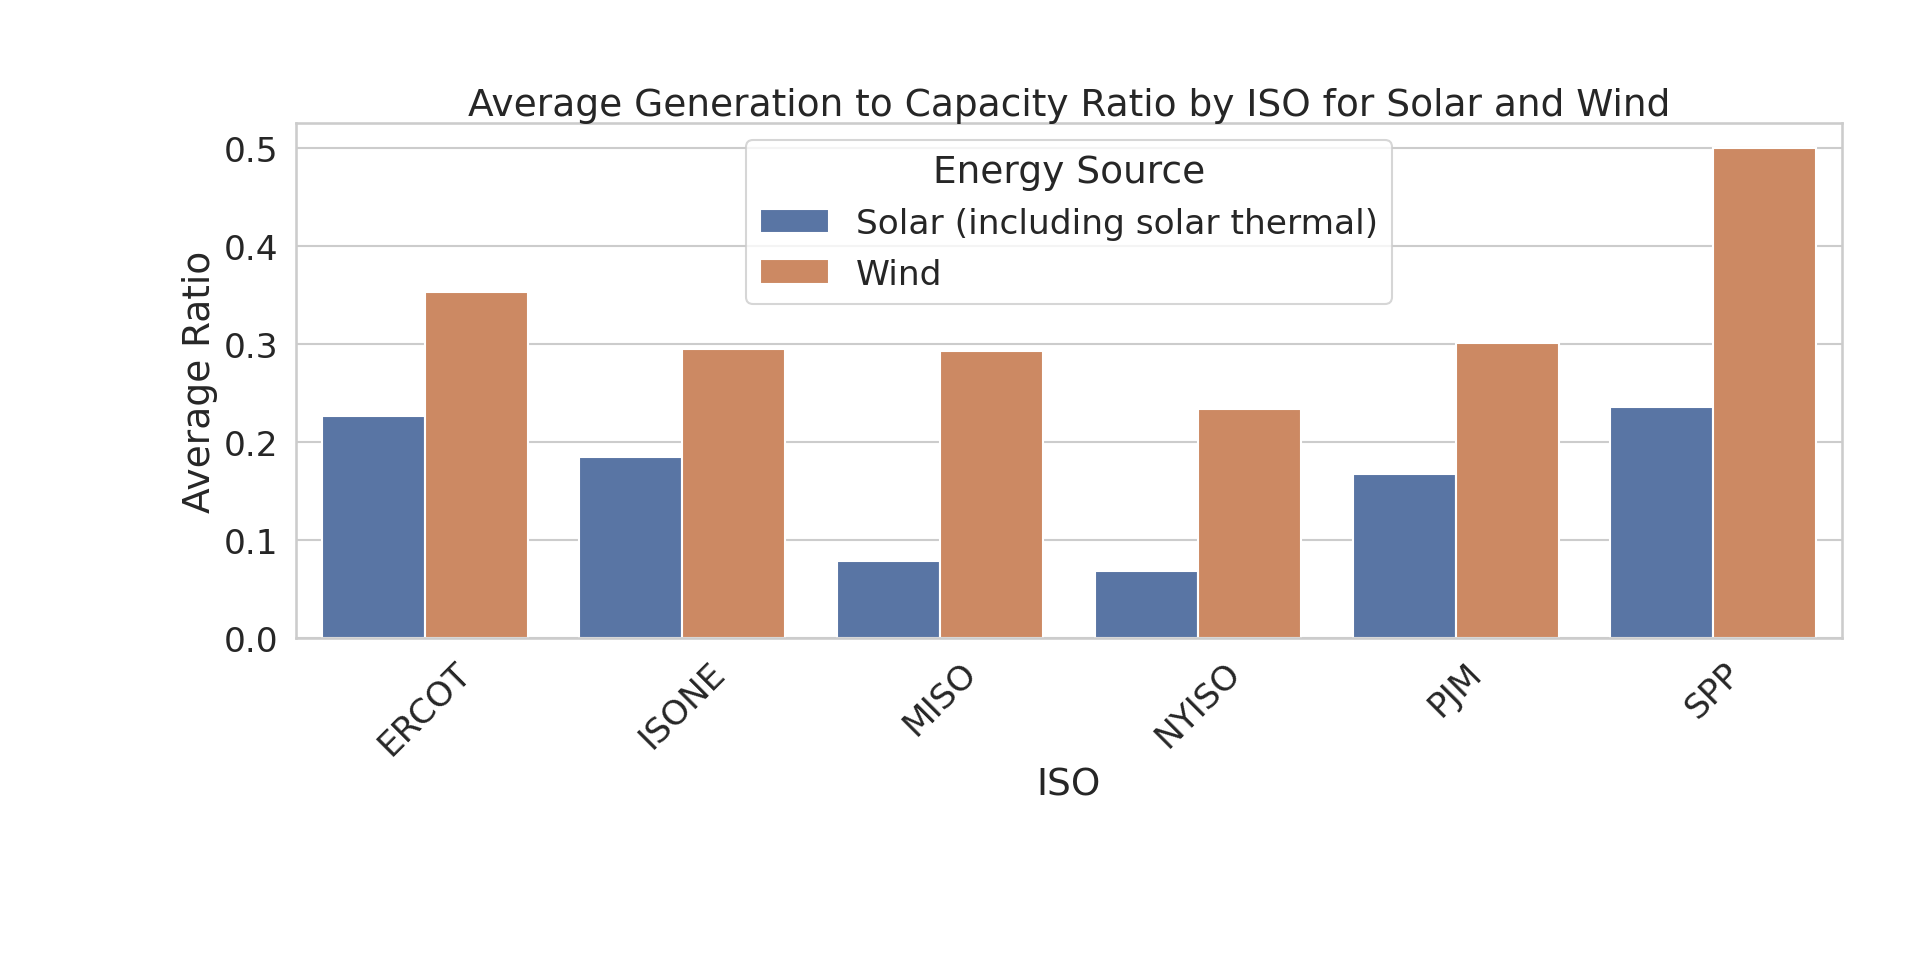
\includegraphics[width=0.5\linewidth]{images/GenerationCapacitySolarWind (1).png}
    \caption{Estimated Capacity Factor for Solar and Wind by ISO.}
    \label{fig:CapacityFactorbyISO}
\end{figure}

\begin{figure}[H]
    \centering
    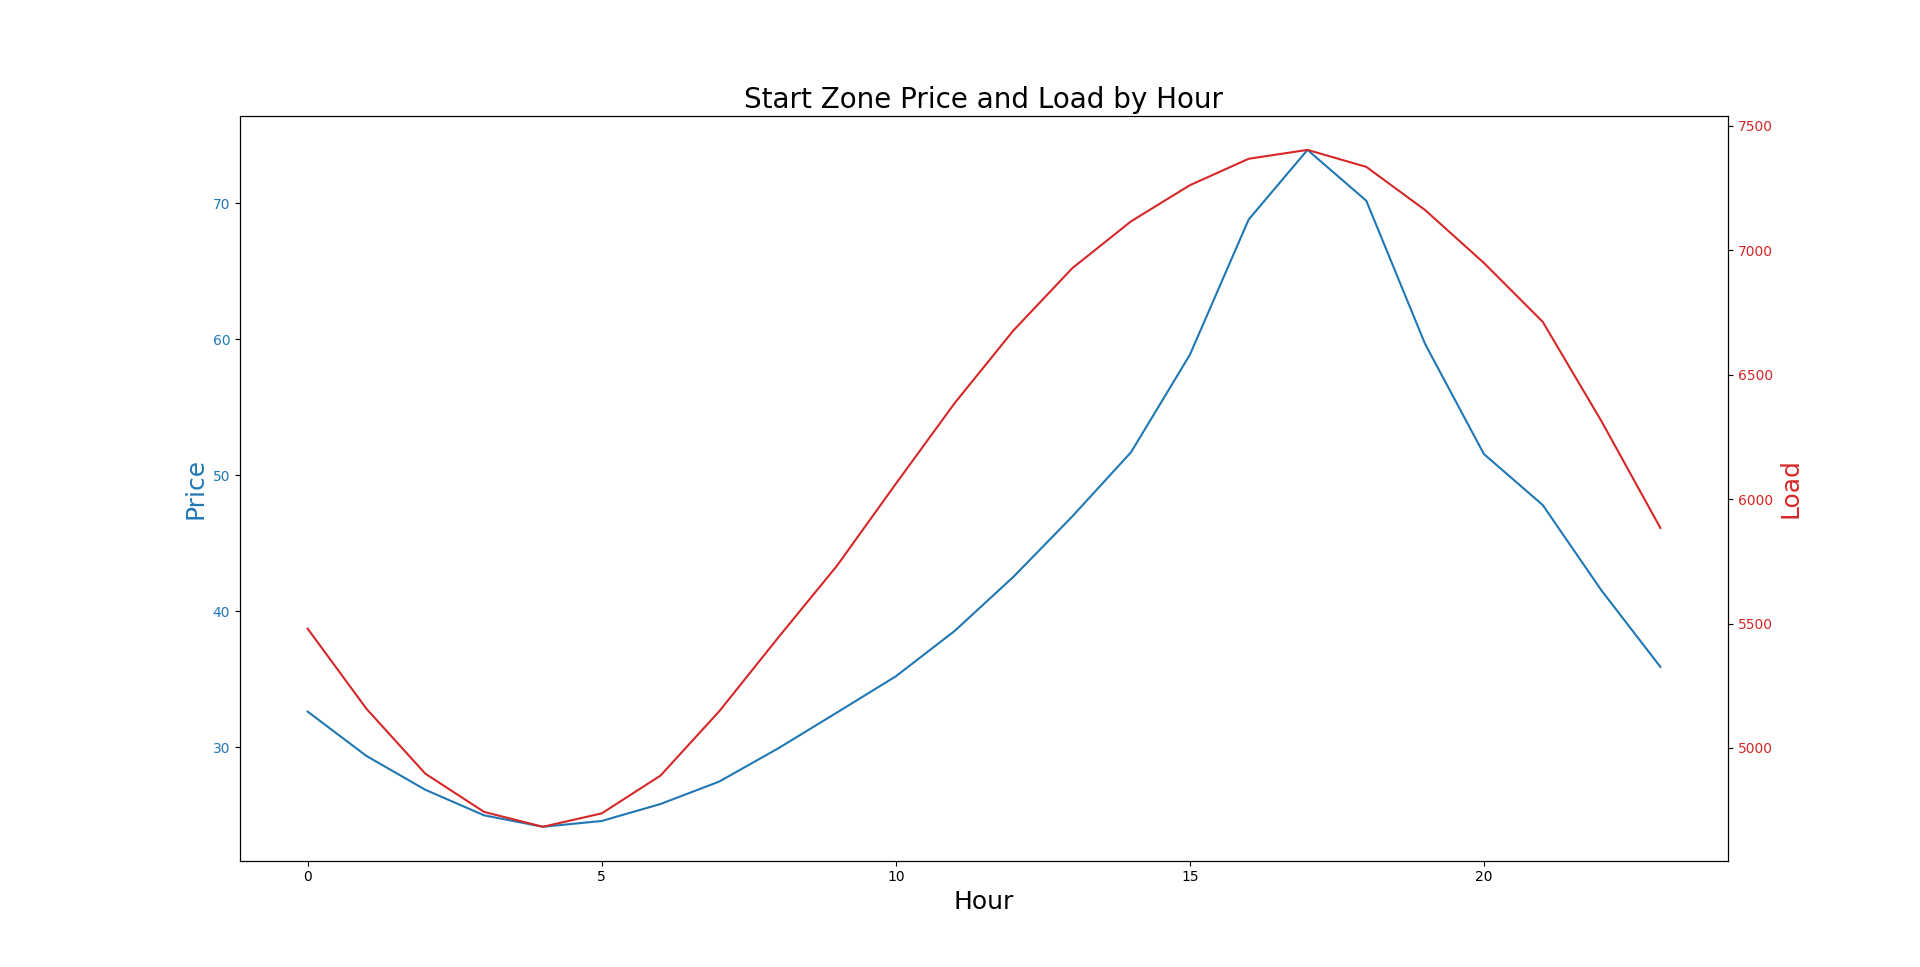
\includegraphics[width=0.5\linewidth]{images/PriceLoadbyHour.png}
    \caption{Price and Load by Hour for entire dataset.}
    \label{fig:PriceLoad}
\end{figure}

\begin{figure}[H]
    \centering
    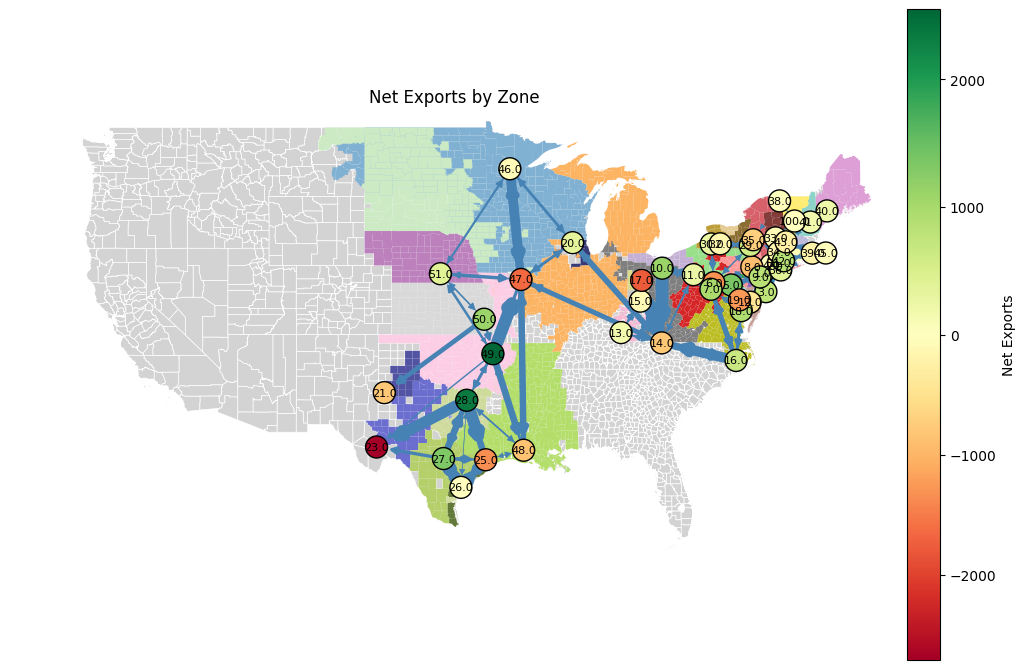
\includegraphics[width=0.5\linewidth]{images/ExportGraph (1).png}
    \caption{Map of Exports between Zones in the Model.}
    \label{ExportGraph}
\end{figure}

% New figures from presentation

\begin{figure}[H]
    \centering
    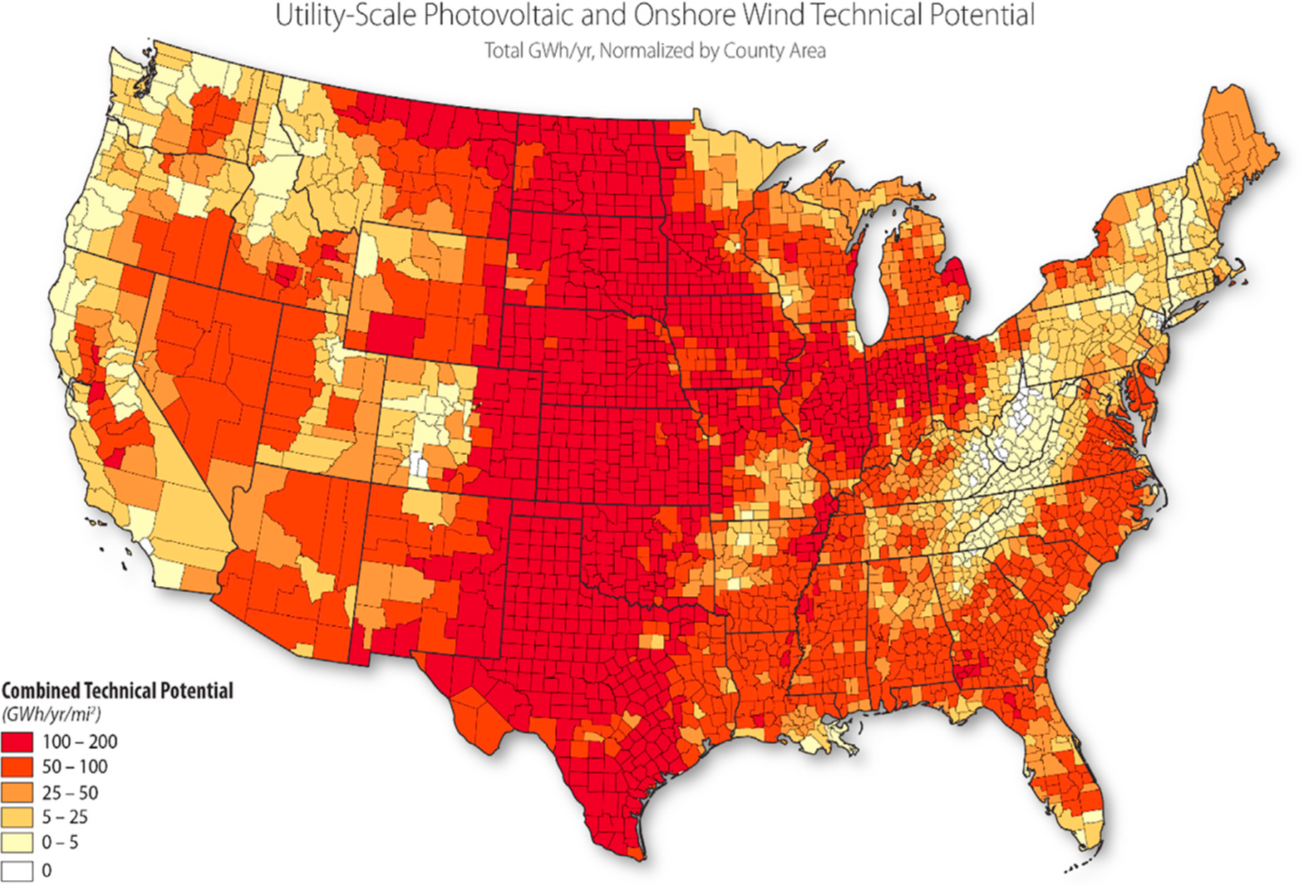
\includegraphics[width=0.8\linewidth]{images/Energy Potential by county.png}
    \caption{Combined Technical Potential for Wind and Solar Generation by County (GWh/yr/mi$^2$). Darker shading indicates higher combined renewable potential. Source: Department of Energy.}
    \label{fig:renewablePotential}
\end{figure}

\begin{figure}[H]
    \centering
    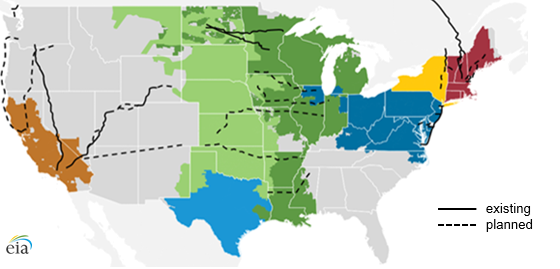
\includegraphics[width=0.8\linewidth]{images/HVDC US.png}
    \caption{Existing and Planned High-Voltage Direct Current Transmission Lines. Solid lines indicate existing HVDC infrastructure; dashed lines indicate proposed expansions. Source: EIA.}
    \label{fig:hvdcLines}
\end{figure}

\begin{figure}[H]
\centering
\begin{tikzpicture}[
    scale=0.55, 
    transform shape,
    gen_node/.style={
        rectangle, 
        draw=black!60, 
        thick, 
        rounded corners=2pt, 
        minimum width=2.6cm, 
        minimum height=2.4cm, 
        align=center, 
        fill=white,
        font=\small
    },
    demand_node/.style={
        circle, 
        draw=blue!70!black, 
        thick, 
        minimum size=2.2cm, 
        fill=blue!5,
        align=center,
        font=\small,
        inner sep=1pt
    },
    fuel_header/.style={
        rectangle, 
        minimum width=2.6cm, 
        minimum height=0.55cm, 
        text=white, 
        font=\bfseries\scriptsize, 
        align=center
    },
    edge_label/.style={
        font=\scriptsize, 
        fill=white, 
        text=black!70,
        rounded corners=1pt,
        draw=black!10,
        inner sep=2pt,
        align=center
    },
    infra_marginal/.style={
        gen_node,
        draw=green!60!black,
        line width=1.5pt,
        fill=green!5
    },
    marginal_gen/.style={
        gen_node,
        draw=orange!90!red,
        line width=2pt,
        fill=orange!5
    },
    extra_marginal/.style={
        gen_node,
        draw=gray!70,
        line width=1.5pt,
        fill=gray!10
    },
    transmission/.style={
        -Latex, 
        thick, 
        draw=blue!50!black
    },
    binding_edge/.style={
        -Latex, 
        line width=2.5pt, 
        draw=red!80!black
    },
    binding_label/.style={
        edge_label,
        text=red!80!black,
        font=\bfseries\scriptsize,
        draw=red!30
    },
    lmp_zero/.style={
        demand_node,
        draw=green!60!black,
        line width=2pt,
        fill=green!10
    },
    lmp_mid/.style={
        demand_node,
        draw=orange!80!red,
        line width=2pt,
        fill=orange!10
    },
    lmp_high/.style={
        demand_node,
        draw=gray!70,
        line width=2pt,
        fill=gray!15
    }
]
    % Supply Layer
    \node[infra_marginal] (j1) at (0, 5) {};
    \node[fuel_header, fill=green!60!black] at ([yshift=0.7cm]j1.center) {Wind};
    \node[align=center, font=\small] at ([yshift=-0.15cm]j1.center) {
        \textbf{Gen $j_1$}\\
        $c_{j_1} = \$0$\\
        Gen: 80 MW
    };

    \node[marginal_gen] (j2) at (6, 5) {};
    \node[fuel_header, fill=orange!80!red] at ([yshift=0.7cm]j2.center) {Gas};
    \node[align=center, font=\small] at ([yshift=-0.15cm]j2.center) {
        \textbf{Gen $j_2$}\\
        $c_{j_2} = \$10$\\
        Gen: 70 MW
    };

    \node[extra_marginal] (j3) at (12, 5) {};
    \node[fuel_header, fill=gray!70] at ([yshift=0.7cm]j3.center) {Coal};
    \node[align=center, font=\small] at ([yshift=-0.15cm]j3.center) {
        \textbf{Gen $j_3$}\\
        $c_{j_3} = \$15$\\
        Gen: 20 MW
    };

    % Demand Layer
    \node[lmp_zero] (i1) at (0, 0) {
        \textbf{Load $i_1$}\\
        $D=60$ MW\\[2pt]
        \textbf{LMP $= \$0$}
    };

    \node[lmp_mid] (i2) at (6, 0) {
        \textbf{Load $i_2$}\\
        $D=70$ MW\\[2pt]
        \textbf{LMP $= \$10$}
    };

    \node[lmp_high] (i3) at (12, 0) {
        \textbf{Load $i_3$}\\
        $D=40$ MW\\[2pt]
        \textbf{LMP $= \$15$}
    };

    % Transmission Flows
    \draw[transmission, line width=1.5pt, draw=green!60!black] (j1.south) -- (i1.north) 
        node[midway, edge_label] {$60 / A=80$};
    \draw[binding_edge, draw=green!50!red] (j1.south east) -- (i2.north west) 
        node[pos=0.25, binding_label] {$\mathbf{20} / \bar{A}=20$};
    \draw[transmission, line width=1.5pt, draw=orange!70!black] (j2.south) -- (i2.north) 
        node[midway, edge_label] {$50 / A=80$};
    \draw[binding_edge, draw=orange!50!red] (j2.south east) -- (i3.north west) 
        node[pos=0.3, binding_label] {$\mathbf{20} / \bar{A}=20$};
    \draw[transmission, line width=1.5pt, draw=gray!70] (j3.south) -- (i3.north) 
        node[midway, edge_label] {$20 / A=40$};

    % Legend
    \node[anchor=north west, align=left, font=\scriptsize, 
          draw=gray!30, rounded corners, fill=white,
          text width=5.5cm] at (6.0, -2.0) {
        \textbf{Legend:}\\[2pt]
        \tikz\draw[green!60!black, line width=1.5pt] (0,0) -- (0.4,0); Wind zone (LMP $= \$0$)\\
        \tikz\draw[orange!90!red, line width=2pt] (0,0) -- (0.4,0); Gas zone (LMP $= \$10$)\\
        \tikz\draw[gray!70, line width=1.5pt] (0,0) -- (0.4,0); Coal zone (LMP $= \$15$)\\
        \tikz\draw[red!80!black, line width=2pt, -Latex] (0,0) -- (0.4,0); Binding constraint ($\bar{A}$)
    };
\end{tikzpicture}
\caption{Network Topology Illustrating Congestion Pricing. Binding export constraints create price separation across zones. Each zone's LMP equals the local marginal cost when transmission constraints bind.}
\label{fig:NetworkTopology}
\end{figure}

\begin{figure}[H]
\centering
\begin{tikzpicture}[econAxis, scale=0.9, transform shape]

    % LEFT PANEL: EXPORTER
    \begin{scope}[local bounding box=LeftPanel]
        \node[above, font=\small\bfseries, align=center] at (2.5, 5.0) {Low-Cost Region\\(Exporter)};
        
        \draw[econAxis] (0,0) -- (5,0) node[below] {$Q$};
        \draw[econAxis] (0,0) -- (0,5) node[left] {$P$};
        
        \draw[supply, name path=S_L] (0,0.5) -- (4.5,4) node[right] {$S_L$};
        \draw[demand, name path=D_L] (1.5,4.5) -- (4,0.5) node[right] {$D_L$};
        
        \path [name intersections={of=S_L and D_L, by=E_L}];
        \draw[priceLine, name path=priceLine_L_old] (0, 1.82) -- (E_L);
        \node[left, font=\footnotesize] at (0, 1.82) {$P_L^0$};
        \fill[gray] (E_L) circle (2.5pt);

        \coordinate (P_trade_L_start) at (0, 2.8);
        \coordinate (P_trade_L_end) at (4.3, 2.8);
        \draw[very thick, color=econGold, name path=Price_L] (P_trade_L_start) -- (P_trade_L_end);
        \node[left, font=\footnotesize, econGold] at (0, 2.8) {$P^*$};
        
        \path [name intersections={of=S_L and Price_L, by=Q_S_new}];
        \path [name intersections={of=D_L and Price_L, by=Q_D_new}];
        
        \begin{scope}[on background layer]
            \fill[econRed!40, opacity=0.7] (0, 1.82) -- (E_L) -- (Q_S_new) -- (0, 2.8) -- cycle;
        \end{scope}
        
        \draw[dotted, gray] (Q_D_new) -- (Q_D_new |- 0,0) node[below, font=\scriptsize] {$Q_D'$};
        \draw[dotted, gray] (Q_S_new) -- (Q_S_new |- 0,0) node[below, font=\scriptsize] {$Q_S'$};
        
        \draw[decorate, decoration={brace, amplitude=5pt, mirror, raise=3pt}, thick, econGold] 
            (Q_D_new |- 0,0) -- (Q_S_new |- 0,0) 
            node[midway, below=10pt, font=\scriptsize, econGold] {\textbf{Exports}};
        
        \draw[-{Stealth[scale=1.2]}, very thick, econGold] (0.6, 1.82) -- (0.6, 2.65);
    \end{scope}

    % RIGHT PANEL: IMPORTER
    \begin{scope}[shift={(7,0)}, local bounding box=RightPanel]
        \node[above, font=\small\bfseries, align=center] at (2.5, 5.0) {High-Cost Region\\(Importer)};
        
        \draw[econAxis] (0,0) -- (5,0) node[below] {$Q$};
        \draw[econAxis] (0,0) -- (0,5) node[left] {$P$};
        
        \draw[supply, name path=S_H] (0,1.5) -- (4.5,4.5) node[below] {$S_H$};
        \draw[demand, name path=D_H] (1,4.5) -- (4.5,0.5) node[below] {$D_H$};
        
        \path [name intersections={of=S_H and D_H, by=E_H}];
        \draw[priceLine] (0,0) |- (E_H);
        \node[left, font=\footnotesize] at (0, 3.35) {$P_H^0$};
        \fill[gray] (E_H) circle (2.5pt);

        \coordinate (P_trade_H_start) at (0, 2.8);
        \coordinate (P_trade_H_end) at (4.3, 2.8);
        \draw[very thick, color=econGold, name path=Price_H] (P_trade_H_start) -- (P_trade_H_end);
        \node[left, font=\footnotesize, econGold] at (0, 2.8) {$P^*$};
        
        \path [name intersections={of=S_H and Price_H, by=Q_S_H_new}];
        \path [name intersections={of=D_H and Price_H, by=Q_D_H_new}];
        
        \begin{scope}[on background layer]
             \fill[econBlue!40, opacity=0.7] (0, 2.8) -- (Q_D_H_new) -- (E_H) -- (0, 3.35) -- cycle;
        \end{scope}

        \draw[dotted, gray] (Q_S_H_new) -- (Q_S_H_new |- 0,0) node[below, font=\scriptsize] {$Q_S'$};
        \draw[dotted, gray] (Q_D_H_new) -- (Q_D_H_new |- 0,0) node[below, font=\scriptsize] {$Q_D'$};

        \draw[decorate, decoration={brace, amplitude=5pt, mirror, raise=3pt}, thick, econGold] 
            (Q_S_H_new |- 0,0) -- (Q_D_H_new |- 0,0) 
            node[midway, below=10pt, font=\scriptsize, econGold] {\textbf{Imports}};

        \draw[-{Stealth[scale=1.2]}, very thick, econGold] (0.6, 3.2) -- (0.6, 2.95);
    \end{scope}

    % CONNECTOR
    \draw[line width=4pt, -{Latex[scale=1.3]}, color=black!50] (5.3, 1.2) -- (6.7, 1.2);
    \node[font=\scriptsize\bfseries, color=black!70] at (6, 1.55) {Flow};

\end{tikzpicture}
\caption{Static Effects of Transmission Expansion: Price Convergence and Spatial Arbitrage. In the low-cost (exporting) region, prices rise and producer surplus increases (red shaded area). In the high-cost (importing) region, prices fall and consumer surplus increases (blue shaded area).}
\label{fig:StaticEffects}
\end{figure}

\begin{figure}[H]
\centering
\begin{tikzpicture}[scale=1.0, econAxis, transform shape]
    
    % Axes
    \draw[econAxis] (0,0) -- (6,0) node[below] {New Capacity ($\Delta K$)};
    \draw[econAxis] (0,0) -- (0,5) node[left] {\$/MW};

    % Marginal Cost
    \draw[supply, name path=MC] (0,1) .. controls (2,1.2) and (4,2.5) .. (5.5,4.8) 
        node[right] {$MC$};

    % MB Original
    \draw[demand, name path=MB0] (0.5,3.5) .. controls (2,3) and (4,1.5) .. (5.5,0.5) 
        node[right] {$MB_{\text{Autarky}}$};

    % MB New
    \draw[demand, densely dashed, line width=1.2pt, name path=MB1] 
        (0.5,4.5) .. controls (2,4) and (4,2.5) .. (5.5,1.5) 
        node[right] {$MB_{\text{Trade}}$};

    % Equilibria
    \path [name intersections={of=MC and MB0, by=E0}];
    \path [name intersections={of=MC and MB1, by=E1}];

    % Drop lines
    \draw[dotted, gray, thick] (E0) -- (E0 |- 0,0) node[below, font=\small] {$K^*_0$};
    \draw[dotted, gray, thick] (E1) -- (E1 |- 0,0) node[below, font=\small] {$K^*_1$};
    
    % Points
    \fill[econBlue] (E0) circle (3.5pt);
    \fill[econRed] (E1) circle (3.5pt);
    \draw[white, line width=1pt] (E0) circle (3.5pt);
    \draw[white, line width=1pt] (E1) circle (3.5pt);
    \fill[econBlue] (E0) circle (3pt);
    \fill[econRed] (E1) circle (3pt);

    % Annotation
    \draw[-{Stealth[scale=1.3]}, very thick, econGold] 
        ($(E0)+(0.15,0.4)$) -- ($(E1)+(-0.15, -0.15)$);
    
    \node[font=\footnotesize, align=left, fill=white, fill opacity=0.85, 
          text opacity=1, inner sep=3pt, rounded corners=2pt] 
        at (1.2, 4.2) 
        {Higher prices\\incentivize entry};

    % Legend
    \node[draw=gray!50, rounded corners=3pt, inner sep=5pt, font=\scriptsize,
          fill=white, anchor=south west] at (0.1, 0.1) {
        \begin{tabular}{@{}cl@{}}
            \textcolor{econBlue}{$\bullet$} & Initial equilibrium \\
            \textcolor{econRed}{$\bullet$} & New equilibrium
        \end{tabular}
    };

    % Capacity expansion
    \draw[{Stealth}-{Stealth}, thick, black!60] 
        ($(E0 |- 0,0) + (0, -0.5)$) -- ($(E1 |- 0,0) + (0, -0.5)$)
        node[midway, below, font=\scriptsize] {$\Delta K^*$};

\end{tikzpicture}
\caption{Dynamic Effects of Transmission Expansion: The Investment Signal. Expanded market access shifts the marginal benefit curve outward for generators in resource-rich regions, leading to increased equilibrium capacity investment.}
\label{fig:DynamicEffects}
\end{figure}

\begin{figure}[H]
\centering
% The resizebox only wraps the tikzpicture
\resizebox{0.98\textwidth}{!}{%
    \begin{tikzpicture}[
        root/.style={
            rectangle, rounded corners=4pt, draw=rootcolor, fill=rootcolor,
            text=white, font=\bfseries\small, minimum height=0.8cm,
            minimum width=3.6cm, align=center
        },
        category/.style={
            rectangle, rounded corners=3pt, draw=#1, fill=#1,
            text=white, font=\bfseries\footnotesize, minimum height=0.65cm,
            minimum width=3.2cm, align=center
        },
        leaf/.style={
            rectangle, rounded corners=2pt, draw=#1!60, fill=leafbg,
            text=black, font=\scriptsize, minimum height=0.55cm,
            minimum width=2.8cm, align=center, inner sep=3pt
        },
        combined/.style={
            rectangle, rounded corners=2pt, draw=catC!60, fill=catC!8,
            text=black, font=\scriptsize\itshape, minimum height=0.55cm,
            minimum width=2.8cm, align=center
        },
        arrow/.style={-{Stealth[length=4pt]}, thick, color=#1},
        note/.style={font=\tiny\itshape, text=black!55, align=center},
    ]

    % Root
    \node[root] (root) at (0,0) {Counterfactual Simulations};

    % ---- Category nodes ----
    \node[category=catA] (catTU) at (-7.85, -1.6) {Transmission Upgrades};
    \node[category=catB] (catNT) at (-0.8, -1.6) {New Long-Distance Lines};
    \node[category=catC] (catFL) at (6.6, -1.6) {Federal Legislation};

    % ---- Transmission Upgrades leaves ----
    \node[leaf=catA] (tu1) at (-9.5, -3.2) {Full HVDC\\[-1pt]Replacement};
    \node[leaf=catA] (tu2) at (-6.2, -3.2) {Partial HVDC\\[-1pt]Replacement};

    % ---- New Transmission leaves ----
    \node[leaf=catB] (nt1) at (-3.5, -3.2) {Remove All\\[-1pt]Constraints};
    \node[leaf=catB] (nt2) at (-0.8, -3.2) {Grain Belt\\[-1pt]Express};
    \node[leaf=catB] (nt3) at (1.9, -3.2) {ERCOT--Eastern\\[-1pt]Interconnection};

    % ---- Federal Legislation leaves ----
    \node[leaf=catC] (fl1) at (4.3, -3.2) {BIG WIRES\\[-1pt]Act};
    \node[leaf=catC] (fl2) at (6.6, -3.2) {Inflation\\[-1pt]Reduction Act};
    \node[leaf=catC] (fl3) at (9.0, -3.2) {Bipartisan\\[-1pt]Infra.\ Law};

    % Combined policy
    \node[combined] (fl4) at (6.6, -5.0) {Combined Policy Effects};

    % ---- Annotations ----
    \node[note] at (-9.5, -4.1) {All inter-zonal lines};
    \node[note] at (-6.2, -4.1) {Random subsets,\\varying intensities};
    \node[note] at (-3.5, -4.1) {Limiting case};
    \node[note] at (-0.8, -4.1) {800-mi HVDC,\\5\,GW from KS};
    \node[note] at (1.9, -4.1) {TX wind/solar\\to Southeast};
    \node[note] at (4.3, -4.15) {MITC $\geq$ 30\%\\peak demand};
    \node[note] at (6.6, -4.15) {ITC + PTC for\\renewables};
    \node[note] at (9.0, -4.15) {Transmission\\grants};
    \node[note] at (6.6, -5.7) {Complementarity test:\\$\Delta W^{\text{joint}}$ vs.\ $\sum \Delta W^{i}$};

    % ---- Welfare Decomposition ----
    \node[category=catD] (wd) at (-7.85, -5.6) {Welfare Decomposition};
    \node[note, right=0.2cm of wd] {Producer/consumer surplus\\by zone; Pareto transfers};

    % ---- Edges: root to categories ----
    \draw[arrow=catA] (root.south) -- ++(0,-0.3) -| (catTU.north);
    \draw[arrow=catB] (root.south) -- ++(0,-0.3) -| (catNT.north);
    \draw[arrow=catC] (root.south) -- ++(0,-0.3) -| (catFL.north);

    % ---- Edges: categories to leaves ----
    \draw[arrow=catA!70] (catTU.south) -- ++(0,-0.2) -| (tu1.north);
    \draw[arrow=catA!70] (catTU.south) -- ++(0,-0.2) -| (tu2.north);

    \draw[arrow=catB!70] (catNT.south) -- ++(0,-0.2) -| (nt1.north);
    \draw[arrow=catB!70] (catNT.south) -- ++(0,-0.2) -| (nt2.north);
    \draw[arrow=catB!70] (catNT.south) -- ++(0,-0.2) -| (nt3.north);

    \draw[arrow=catC!70] (catFL.south) -- ++(0,-0.2) -| (fl1.north);
    \draw[arrow=catC!70] (catFL.south) -- ++(0,-0.2) -| (fl2.north);
    \draw[arrow=catC!70] (catFL.south) -- ++(0,-0.2) -| (fl3.north);

    % Dashed to combined
    \draw[dashed, catC!50, thick] (fl1.south) |- (fl4.west);
    \draw[dashed, catC!50, thick] (fl2.south) -- (fl4.north);
    \draw[dashed, catC!50, thick] (fl3.south) |- (fl4.east);

    % Welfare decomposition arrow (dashed from root)
    \draw[arrow=catD, dashed] (root.south) -- ++(0,-0.3) -- ++(-7.85, 0) |- (wd.north);

    \end{tikzpicture}%
} % End of resizebox

\caption{Visual description of counterfactuals run and how they relate.}
\label{fig:CounterfactualSimulations}

\end{figure}


%\begin{figure}[hp]
%  \centering
%  \includegraphics[width=.6\textwidth]{../fig/placeholder.pdf}
%  \caption{Placeholder}
%  \label{fig:placeholder}
%\end{figure}




\clearpage

\appendix

\section{Solving the Operations Model}\label{app:operations}

This appendix derives the likelihood function used to estimate the short-run operations model. Section~\ref{app:iso_problem} establishes the equivalence between the generator profit maximization problem and a social planner's cost minimization problem, then formulates the ISO's dispatch problem. Section~\ref{app:focs} derives the first-order conditions from the Lagrangian. Section~\ref{app:likelihood} specifies the cost function and derives the likelihood function for estimation.

\subsection{The ISO Dispatch Problem}\label{app:iso_problem}

Under standard conditions, the generator's profit maximization problem is equivalent to a social planner's cost minimization problem. Following \cite{gilbert2004allocating} and \cite{cramton2017electricity}, the conditions for this equivalence include: (i) no market power among generators, (ii) no gamesmanship or non-competitive bidding, (iii) increasing marginal cost curves, and (iv) linear constraints. The assumption of increasing marginal costs is consistent with both bid offer data and economic theory. Gamesmanship and non-competitive bidding are prohibited and actively monitored by the Federal Energy Regulatory Commission. While transmission constraints can create local market power (\cite{gilbert2004allocating}), competitive pressures and regulatory limits on bidding behavior make sustained market power difficult to maintain.

I aggregate to the resource and ISO level due to data limitations: hourly generation data are available only at the resource level rather than the generator level. While this aggregation sacrifices granularity that would be valuable in a transmission model, I disaggregate where data permit.

\subsubsection{Notation}

Let $i \in \{1, \ldots, I\}$ index demand nodes, $j \in \{1, \ldots, J\}$ index supply (generation) nodes, $k \in \{1, \ldots, K\}$ index resources at each supply node, and $t \in \{1, \ldots, T\}$ index time periods (hours). Define:
\begin{itemize}
    \item $q_{ijkt}$: Quantity of electricity sent from resource $k$ at supply node $j$ to demand node $i$ at time $t$
    \item $c_{jkt}(\cdot)$: Cost function for resource $k$ at supply node $j$ at time $t$
    \item $x_{jkt}$: Observable cost shifters for resource $jk$ at time $t$
    \item $\epsilon_{ijkt}$: Unobserved cost shock
    \item $A_{ij}$: Transmission capacity between nodes $i$ and $j$
    \item $O_{jkt}^{MAX}$: Maximum generation capacity of resource $k$ at node $j$ at time $t$
    \item $L_{it}$: Load (demand) at node $i$ at time $t$
    \item $B_{ij}$: Transmission loss factor between nodes $i$ and $j$
\end{itemize}

\subsubsection{The Optimization Problem}

The ISO solves a static cost minimization problem each hour, choosing dispatch quantities $q_{ijkt}$ to minimize the total cost of meeting demand:
\begin{equation}\label{eq:objective}
    \pi_{t} = \max_{\{q_{ijkt}\}} \left[ -\sum_{j=1}^{J} \sum_{k=1}^{K} c_{jkt}\left(x_{jkt}, \sum_{i=1}^{I} q_{ijkt}, \sum_{i=1}^{I} \epsilon_{ijkt}\right) \right]
\end{equation}
subject to three constraints.

\paragraph{Transmission Constraint.} Flows between any two nodes cannot exceed line capacity:
\begin{equation}\label{eq:transmission}
    \sum_{k=1}^{K} q_{ijkt} \leq A_{ij} \quad \forall \, i, j, t.
\end{equation}

\paragraph{Capacity Constraint.} Total dispatch from each resource cannot exceed its maximum capacity:
\begin{equation}\label{eq:capacity}
    0 \leq \sum_{i=1}^{I} q_{ijkt} \leq O_{jkt}^{MAX} \quad \forall \, j, k, t.
\end{equation}

\paragraph{Load Balance Constraint.} Supply must equal demand at each node, accounting for transmission losses:
\begin{equation}\label{eq:load_balance}
    \sum_{j=1}^{J} \sum_{k=1}^{K} (1 - B_{ij}) q_{ijkt} = L_{it} \quad \forall \, i, t.
\end{equation}

Three maintained assumptions ensure the problem is well-defined: (i) no blackouts, meaning sufficient generation capacity exists to serve all load at every node; (ii) no resource is transmission-constrained to all destinations; and (iii) at least one resource at each generation node has slack capacity at any given time.

When no constraints bind, resources set marginal cost equal to price and serve the highest-priced locations first. When the transmission constraint binds, a resource dispatches up to $A_{ij} - \sum_{k' \neq k} q_{ijk't}$ units to the highest-priced location, then up to $A_{ij}$ units to the next highest-priced location, continuing until either maximum capacity $O_{jkt}^{MAX}$ is reached or marginal revenue equals marginal cost. Prices equal the marginal cost of the last economically dispatched resource at each location.

\subsection{First-Order Conditions}\label{app:focs}

The Lagrangian for the ISO's problem at time $t$ is:
\begin{align}\label{eq:lagrangian}
    \mathcal{L}_t = & -\sum_{k=1}^{K} \sum_{j=1}^{J} c_{jkt}\left(x_{jkt}, \sum_{i=1}^{I} q_{ijkt}, \sum_{i=1}^{I} \epsilon_{ijkt}\right) \nonumber \\
    & + \sum_{i,j} \lambda_{ijt} \left(A_{ij} - \sum_{k=1}^{K} q_{ijkt}\right) \nonumber \\
    & + \sum_{i} \gamma_{it} \left(L_{it} - \sum_{k=1}^{K} \sum_{j=1}^{J} (1 - B_{ij}) q_{ijkt}\right) \nonumber \\
    & + \sum_{j,k} \theta_{jkt} \left(O_{jkt}^{MAX} - \sum_{i=1}^{I} q_{ijkt}\right),
\end{align}
where $\lambda_{ijt}$ is the multiplier on the transmission constraint, $\gamma_{it}$ is the multiplier on the load balance constraint, and $\theta_{jkt}$ is the multiplier on the capacity constraint.

\subsubsection{Optimality Conditions}

The first-order condition with respect to $q_{ijkt}$ is:
\begin{equation}\label{eq:foc}
    \frac{\partial \mathcal{L}_t}{\partial q_{ijkt}} = -\frac{\partial c_{jkt}}{\partial q_{ijkt}} - \lambda_{ijt} - \gamma_{it}(1 - B_{ij}) - \theta_{jkt} = 0.
\end{equation}

Complementary slackness requires:
\begin{align}
    \lambda_{ijt} \left(A_{ij} - \sum_{k=1}^{K} q_{ijkt}\right) &= 0 \quad \forall \, i, j, t, \label{eq:cs_trans} \\
    \theta_{jkt} \left(O_{jkt}^{MAX} - \sum_{i=1}^{I} q_{ijkt}\right) &= 0 \quad \forall \, j, k, t. \label{eq:cs_cap}
\end{align}

Rearranging equation~\eqref{eq:foc} yields three equivalent expressions:
\begin{align}
    \frac{\partial c_{jkt}}{\partial q_{ijkt}} + \gamma_{it}(1 - B_{ij}) + \theta_{jkt} &= \lambda_{ijt}, \label{eq:foc_lambda} \\
    \frac{\partial c_{jkt}}{\partial q_{ijkt}} + \gamma_{it}(1 - B_{ij}) + \lambda_{ijt} &= \theta_{jkt}, \label{eq:foc_theta} \\
    \frac{\partial c_{jkt}}{\partial q_{ijkt}} + \lambda_{ijt} + \theta_{jkt} &= \gamma_{it}(1 - B_{ij}). \label{eq:foc_gamma}
\end{align}

\subsubsection{Intratemporal Euler Conditions}

Three key relationships emerge from comparing first-order conditions across different resource-node combinations.

\paragraph{Condition 1: Same supply node, different resources.} For two resources $k$ and $k'$ at the same supply node $j$, both sending to demand node $i$:
\begin{equation}\label{eq:euler1}
    \frac{\partial c_{jkt}}{\partial q_{ijkt}} + \theta_{jkt} = \frac{\partial c_{jk't}}{\partial q_{ijk't}} + \theta_{jk't}.
\end{equation}

\paragraph{Condition 2: Same resource, different demand nodes.} For resource $k$ at supply node $j$ sending to two demand nodes $i$ and $i'$:
\begin{equation}\label{eq:euler2}
    \frac{\partial c_{jkt}}{\partial q_{ijkt}} + \gamma_{it}(1 - B_{ij}) + \lambda_{ijt} = \frac{\partial c_{jkt}}{\partial q_{i'jkt}} + \gamma_{i't}(1 - B_{i'j}) + \lambda_{i'jt}.
\end{equation}

\paragraph{Condition 3: Different supply nodes, same demand node.} For resources at different supply nodes $jk$ and $j'k'$ both sending to demand node $i$:
\begin{equation}\label{eq:euler3}
    \frac{\partial c_{jkt}}{\partial q_{ijkt}} + \lambda_{ijt} + \theta_{jkt} = \frac{(1 - B_{ij})}{(1 - B_{ij'})} \left[\frac{\partial c_{j'k't}}{\partial q_{ij'k't}} + \lambda_{ij't} + \theta_{j'k't}\right].
\end{equation}

\subsection{Cost Function Specification and Likelihood}\label{app:likelihood}

\subsubsection{Cost Function}

For renewable resources (wind and solar), the cost function is linear in output:
\begin{equation}
    c_{jkt}^{renew} = q_{ijkt} \epsilon_{ijkt}.
\end{equation}

For non-renewable resources, the cost function is quadratic:
\begin{equation}\label{eq:cost_nonrenew}
    c_{jkt} = \sum_{i=1}^{I} q_{ijkt} x_{jkt} \beta + \frac{1}{2} \left(\sum_{i=1}^{I} q_{ijkt}\right)^2 \nu_k + \sum_{i=1}^{I} q_{ijkt} \epsilon_{ijkt},
\end{equation}
where $\beta$ and $\nu_k$ are parameters to be estimated, with $\nu_k$ varying by resource type to capture differences in fuel costs. The marginal cost for non-renewable resources is:
\begin{equation}\label{eq:mc}
    \frac{\partial c_{jkt}}{\partial q_{ijkt}} = x_{jkt} \beta + q_{ijkt} \nu_k + \epsilon_{ijkt}.
\end{equation}

\subsubsection{Identifying the Central Resource}

Define a \emph{central resource} at each demand node as a resource for which neither the transmission constraint nor the capacity constraint binds: $\lambda_{ijt} = 0$ and $\theta_{jkt} = 0$. By the no-blackout assumption, every demand node has at least one central resource. For central resources, the observed locational marginal price (LMP) equals marginal cost:
\begin{equation}
    \frac{\partial c_{jkt}}{\partial q_{ijkt}} = LMP_{it}.
\end{equation}

Using equation~\eqref{eq:euler3} with a central resource $j''k''$ at node $i$:
\begin{equation}\label{eq:central}
    \frac{\partial c_{jkt}}{\partial q_{ijkt}} + \lambda_{ijt} + \theta_{jkt} = \frac{(1 - B_{ij})}{(1 - B_{ij''})} LMP_{it}.
\end{equation}

Rearranging and substituting the marginal cost specification:
\begin{equation}\label{eq:error_eq}
    x_{jkt} \beta + q_{ijkt} \nu_k + \lambda_{ijt} + \theta_{jkt} - \frac{(1 - B_{ij})}{(1 - B_{ij''})} LMP_{it} = -\epsilon_{ijkt}.
\end{equation}

\subsubsection{Solving for Shadow Prices}

From equation~\eqref{eq:foc_gamma} applied to the central resource at node $i$:
\begin{equation}\label{eq:gamma}
    \gamma_{it} = \frac{LMP_{it}}{(1 - B_{ij''})}.
\end{equation}

\paragraph{Transmission Shadow Price.} Using equation~\eqref{eq:euler2} and the assumption that each resource can send electricity to at least one unconstrained destination $i'$ (so $\lambda_{i'jt} = 0$):
\begin{equation}\label{eq:lambda}
    \lambda_{ijt} = q_{i'jkt} \nu_k - q_{ijkt} \nu_k + \frac{LMP_{i't}}{(1 - B_{i'j''})}(1 - B_{i'j}) - \frac{LMP_{it}}{(1 - B_{ij'''})}(1 - B_{ij}) + \epsilon_{i'jkt} - \epsilon_{ijkt},
\end{equation}
where $j''$ and $j'''$ denote the central resources at nodes $i'$ and $i$, respectively.

\paragraph{Capacity Shadow Price.} Using equation~\eqref{eq:euler1} and the assumption that each generation node has at least one resource $k'$ with slack capacity (so $\theta_{jk't} = 0$):
\begin{equation}\label{eq:theta}
    \theta_{jkt} = (x_{jk't} \beta + q_{ijk't} \nu_{k'}) - (x_{jkt} \beta + q_{ijkt} \nu_k) + \epsilon_{ijk't} - \epsilon_{ijkt}.
\end{equation}

\subsubsection{Constructing the Likelihood Function}

Substituting the expressions for $\lambda_{ijt}$ and $\theta_{jkt}$ into equation~\eqref{eq:error_eq} yields the estimating equation. Define the composite error:
\begin{equation}\label{eq:composite_error}
    \tilde{\epsilon}_{ijkt} = \epsilon_{ijkt} - \epsilon_{i'jkt} - \epsilon_{ijk't},
\end{equation}
where $i'$ is the unconstrained destination for resource $jk$ and $k'$ is the unconstrained resource at node $j$.

The deterministic component of the estimating equation is:
\begin{align}\label{eq:V}
    \tilde{V}_{ijkt} = \; & \underbrace{x_{jkt} \beta + q_{ijkt} \nu_k}_{\text{MC of resource } jk} - \underbrace{\frac{(1 - B_{ij})}{(1 - B_{ij''})} LMP_{it}}_{\text{MC of central resource}} \nonumber \\
    & + \underbrace{q_{i'jkt} \nu_k - q_{ijkt} \nu_k + \frac{LMP_{i't}}{(1 - B_{i'j''})}(1 - B_{i'j}) - \frac{LMP_{it}}{(1 - B_{ij'''})}(1 - B_{ij})}_{\text{cost of transmission constraint}} \nonumber \\
    & + \underbrace{(x_{jk't} \beta + q_{ijk't} \nu_{k'}) - (x_{jkt} \beta + q_{ijkt} \nu_k)}_{\text{cost of capacity constraint}}.
\end{align}

For resources with transmission constraints but no capacity constraints:
\begin{equation}
    \tilde{\epsilon}_{ijk't} = \epsilon_{ijk't} - \epsilon_{i'jk't}.
\end{equation}

For resources with neither constraint binding:
\begin{equation}
    \tilde{\epsilon}_{i'jk't} = \epsilon_{i'jk't}.
\end{equation}

By substitution, each individual error $\epsilon_{ijkt}$ can be recovered.

\subsubsection{Maximum Likelihood Estimation}

Let $P_t(\cdot)$ denote a multivariate normal density with mean zero and variance-covariance matrix $\Omega$. The likelihood function is:
\begin{equation}\label{eq:likelihood}
    \mathcal{L} = \prod_{t=1}^{T} P_t\left(\tilde{V}_{111t}, \ldots, \tilde{V}_{IJKt}\right).
\end{equation}

Maximizing this likelihood function yields estimates of $\beta$ (the effect of observable cost shifters) and $\nu_k$ (resource-type-specific marginal cost parameters), thereby recovering the short-run cost structure.

\section{Long-run Model Computational Details} \label{sec:appendixb}
\addcontentsline{toc}{section}{Appendix B: Long-run Model Computational Details}

\subsection{Algorithm Overview}\label{sec:algorithm_overview}

This appendix details the computational methodology for estimating the long-run capacity investment model. The estimation combines a nested fixed point algorithm for computing equilibrium with generalized method of moments (GMM) estimation for parameter recovery. The approach follows the dynamic game estimation methodology developed by \cite{pakes1998empirical} and utilizes algorithmic improvements from \cite{gowrisankaran2024computable} to identify feasible choices and accelerate convergence.

The computational procedure consists of three main components: (i) state space discretization, (ii) equilibrium computation via nested fixed point iteration, and (iii) GMM estimation using simulated moments. Each component is described in detail below.

\subsection{State Space Discretization}\label{sec:state_space}

The dynamic investment problem is solved over a discretized approximation to the continuous state space. Discretization renders the Bellman equation computationally tractable while preserving economically relevant variation in prices, quantities, and profits. The grid is constructed to capture empirically observed ranges of capacity, demand, and prices, with bounds chosen to exceed historical maxima to accommodate counterfactual investment paths.

\subsubsection{State Variable Bins}\label{subsec:state_bins}

The state space is discretized as shown in Table \ref{tab:state_space}. Each state variable is discretized using evenly spaced bins over a bounded interval informed by historical data and engineering constraints.

\begin{table}[htbp]
\centering
\caption{State Space Discretization}
\label{tab:state_space}
\begin{tabular}{lcc}
\toprule
State Variable & Bins & Range \\
\midrule
Fixed cost ($F_k$) & 20 & $[0, \bar{R}_k]$ \\
Entry cost ($E_k$) & 20 & $[0, 10 \times \bar{R}_k]$ \\
Demand state & 5 & $[0.75 \times \bar{L}, 1.5 \times \bar{L}]$ \\
Own capacity ($O_{jkg}$) & 15 & $[0, 1.5 \times \bar{G}_{jg}]$ \\
Rival capacity ($O_{jkg}^-$) & 10 & $[0, 1.5 \times \bar{L}]$ \\
Average price ($P_{jkg}$) & 10 & $[0, 1.1 \times \bar{P}]$ \\
\bottomrule
\end{tabular}
\begin{minipage}{0.9\textwidth}
\vspace{0.5em}
\footnotesize
\textit{Notes:} $\bar{R}_k$ denotes maximum observed revenue per MW for resource type $k$; $\bar{L}$ denotes the historical maximum system load; $\bar{G}_{jg}$ denotes the maximum observed generation by owner $g$ in region $j$; and $\bar{P}$ denotes the historical maximum average price.
\end{minipage}
\end{table}

Demand uncertainty is modeled using a multiplicative demand scaling factor applied to historical load profiles. The five demand states span $\pm 25\%$ around baseline demand and are intended to capture persistent variation in system conditions rather than transitory hourly shocks.

Own capacity and rival capacity are discretized separately. Own capacity reflects firm-specific investment decisions, while rival capacity aggregates the competitive fringe and other strategic firms into a single state variable, consistent with an oblivious equilibrium approximation. Capacity bounds exceed historical maxima to allow for endogenous entry and expansion in counterfactual scenarios.

\subsubsection{Short-Run Outcome Mapping}

For each point in the discretized state space, the model computes short-run equilibrium outcomes by solving a linear or quadratic dispatch problem subject to generator capacity constraints, zonal load balance, and transmission limits (see Section \ref{sec:appendixc}). The solution yields locational marginal prices, dispatched quantities, production costs, and operating profits.

Outcomes are computed as weighted averages across representative operating conditions (e.g., seasonal or load-duration blocks), producing a smooth mapping from state variables to expected period profits. These expected profits are stored and treated as primitives in the dynamic investment problem.

\subsubsection{Investment Choice Set}

The firm’s investment choice is restricted to a discrete set of ten capacity adjustment options. These include incremental additions for expanding technologies and retirement options for declining resources. Capacity is constrained to remain weakly non-negative, ruling out infeasible states. This restriction substantially reduces the dimensionality of the choice set while preserving the economically relevant margins of adjustment.

\subsubsection{Approximation Accuracy and Computational Feasibility}

The number of bins for each state variable reflects a tradeoff between approximation accuracy and computational feasibility. Finer grids are used for own capacity and cost states, which directly affect firm profits, while coarser grids are used for rival capacity and prices. Sensitivity checks using alternative grid densities yield similar qualitative investment patterns, indicating that results are not driven by discretization artifacts.

The full state space is evaluated using batched computation with intermediate checkpointing, enabling parallel execution and recovery from job interruption. This approach allows the model to evaluate tens of thousands of state points per resource type while maintaining feasible memory and runtime requirements. A schematic overview of the dataset construction is provided in Figure \ref{DataSetCreation}.

\subsection{Equilibrium Computation}\label{sec:equilibrium}

This section describes the numerical procedure used to compute equilibrium investment behavior in the dynamic oligopoly model. The equilibrium is solved using a nested fixed point algorithm, combining backward induction over time with an outer loop over firms’ beliefs about rival behavior.

\subsubsection{Nested Fixed Point Procedure}\label{subsec:nfxp}

The equilibrium is computed through a nested fixed point procedure. The outer loop iterates on beliefs over rival investment behavior until beliefs are consistent with optimal policies, while the inner loop solves each firm’s dynamic programming problem conditional on these beliefs.

This approach follows the standard structure of dynamic oligopoly models with forward-looking firms and strategic interactions, and is computationally necessary given the high-dimensional state space.

\vspace{1em}
\noindent\textbf{Algorithm (Outer Loop):}
\begin{enumerate}
\item \textit{Initialize beliefs:} Each generation company initializes beliefs over the probability distribution of rival investment actions. Beliefs are defined over aggregate rival capacity changes rather than individual firm actions, consistent with the equilibrium concept described below.

\item \textit{Value function iteration:} Conditional on these beliefs, each firm solves its dynamic optimization problem via backward induction. This inner loop yields optimal investment policies and associated value functions for all states.

\item \textit{Update beliefs:} Beliefs are updated using the implied distribution of investment actions generated by firms’ optimal policies.

\item \textit{Check convergence:} The procedure iterates until the maximum deviation between successive policy functions satisfies
\[
    \max |\sigma^{(n+1)} - \sigma^{(n)}| < \epsilon.
\]
If convergence is not achieved, the algorithm returns to Step 2.


\end{enumerate}

Convergence is assessed jointly over value functions and policy functions to ensure stability of both expected payoffs and equilibrium behavior.

\subsubsection{Equilibrium Concept}\label{subsec:equilibrium_concept}

Rather than solving for a full Markov Perfect Equilibrium (MPE), I employ an oblivious equilibrium concept. Under this approach, firms condition their decisions on their own state variables and a low-dimensional summary of competitors’ states, namely the distribution of aggregate rival competitive capacity.

Firms do not track the full joint distribution of rival capacities across individual competitors. Instead, beliefs must be correct with respect to the evolution of total rival capacity. This substantially reduces the dimensionality of the state space while preserving the key strategic channel through which rivals’ investment decisions affect prices and profits.

This approximation is particularly well suited to electricity markets, where individual generators are small relative to the market but investment decisions influence prices through aggregate capacity.

\subsubsection{Value Function Solution}\label{subsec:value_function}

In the final period $T$, firms solve a stationary problem with no further investment opportunities. The value function is given by:

\begin{equation}\label{eq:value_function}
    \upsilon_{jgT}(\Omega) = \max_{\Delta O_{jkg}} \left\{ \Pi_{jg}(\Omega) + \sum_k \varepsilon_{jkg}(\Delta O_{jkg}) + \frac{1}{1-\beta} \Pi_{jg}'(\Omega') \right\}
\end{equation}
subject to the law of motion for capacity:
\begin{equation}
    O_{jkg}' = O_{jkg} + \Delta O_{jkg} \quad \forall k
\end{equation}

The state vector $\Omega$ includes firm-specific capacity holdings, demand conditions, and cost states. The term $\varepsilon_{jkg}$ represents an idiosyncratic choice shock that smooths the policy function and ensures well-defined choice probabilities in the numerical implementation. The final period is treated as stationary with no further capacity investments, so firms receive the discounted perpetuity of steady-state profits.

The final period is treated as stationary: after period $T$, firms receive the discounted perpetuity of steady-state profits conditional on post-investment capacity levels.


Period profits are defined as:
\begin{equation}\label{eq:profits}
\begin{split}
    \Pi_{jg} = \sum_k \Big[ & D_{jkg}(d_{jkg}, O_{jkg}, O_{jkg}^-) P_{jkg} - C_{jkg}(d_{jkg}, O_{jkg}, O_{jkg}^-) D_{jkg}(d_{jkg}, O_{jkg}, O_{jkg}^-) \\
    & - F_k O_{jkg} - E_k \max(\Delta O_{jkg}, 0) \Big]
\end{split}
\end{equation}
where $D_{jkg}$ is dispatch, $P_{jkg}$ is price, $C_{jkg}$ is variable cost, $F_k$ is per-period fixed cost, and $E_k$ is entry cost for new capacity.

Prices, dispatch, and variable costs are outcomes of a short-run operations model that clears the electricity market given total installed capacity and demand conditions. Fixed costs are incurred on all installed capacity, while entry costs apply only to new investment.

\subsubsection{First-Order Conditions}\label{subsec:foc}

Ignoring the non-differentiable choice shock term, the first-order condition with respect to $\Delta O_{jkg}$ is:
\begin{equation}\label{eq:foc}
\frac{\partial \upsilon_{jgT}}{\partial \Delta O_{jkg}}
= \frac{\partial \Pi_{jkg}}{\partial \Delta O_{jkg}}
+ \frac{1}{1-\beta} \frac{\partial \Pi_{jkg}'}{\partial \Delta O_{jkg}}
= 0.
\end{equation}

For capacity reductions, $\max(\Delta O_{jkg},0)=0$, yielding:
\begin{equation}\label{eq:reducing_capacity}
\frac{\partial \left[ D_{jkg}' P_{jkg}' - C_{jkg}' D_{jkg}' \right]}{\partial \Delta O_{jkg}} = F_k.
\end{equation}

For capacity expansions, $\max(\Delta O_{jkg},0)=\Delta O_{jkg}$:
\begin{equation}\label{eq:increasing_capacity}
E_k + \frac{\beta}{1-\beta} F_k
= \frac{\beta}{1-\beta}
\frac{\partial \left[ D_{jkg}' P_{jkg}' - C_{jkg}' D_{jkg}' \right]}{\partial \Delta O_{jkg}}.
\end{equation}

The derivatives of dispatch, prices, and costs with respect to capacity are well defined because the short-run operations problem is a linear program. Sensitivity of equilibrium outcomes to capacity constraints can therefore be computed using standard LP dual variables.

\subsubsection{Handling Multiple Equilibria}\label{subsec:multiple_equilibria}

The dynamic investment game may admit multiple equilibria. I impose a sequential move structure within each period, where firms move in descending order of installed capacity. The largest incumbent firm chooses its investment first, followed sequentially by smaller firms.

This equilibrium selection rule both reduces multiplicity and reflects empirical patterns in electricity markets, where large incumbents typically lead capacity expansion decisions.

\subsubsection{Backward Induction}\label{subsec:backward_induction}
For periods $t < T$, the model is solved via backward induction. Relative to the terminal period, two features differ:

\begin{enumerate}
\item Firms account for expectations over future profit streams conditional on stochastic evolution of demand and cost states.
\item Capacity adjustment costs enter through the parameter $\psi_{1k}$, affecting average fixed costs and smoothing intertemporal investment behavior.
\end{enumerate}

Expected continuation values are computed by integrating over discretized transition kernels for exogenous state variables and deterministic capacity evolution.

\subsection{GMM Estimation}\label{sec:gmm}

\subsubsection{Parameter Space}\label{subsec:parameters}

The long-run model contains 32 parameters to estimate. For each of the four resource types $k \in \{\text{natural gas, coal, solar, wind}\}$, the parameters include:

\begin{itemize}
    \item \textbf{Fixed cost process:} initial value ($F_k^0$), autoregressive coefficient ($\rho_k^F$), innovation standard deviation ($\sigma_k^F$), and integrated component coefficient
    \item \textbf{Entry cost process:} initial value ($E_k^0$), autoregressive coefficient ($\rho_k^E$), innovation standard deviation ($\sigma_k^E$), and integrated component coefficient
\end{itemize}

\subsubsection{Moment Conditions}\label{subsec:moments}

The estimation uses 36 moment conditions to identify the 32 parameters, yielding an overidentified model. Following \cite{gowrisankaran2024energy}, the moment conditions are constructed to capture key features of the investment distribution.

\vspace{1em}
\noindent\textbf{For natural gas, solar, and wind resources:}
\begin{itemize}
    \item $\mathbbm{1}(\Delta O_{jkg} > 0) \times \Delta O_{jkg}$ — positive investment indicator interacted with quantity
    \item $(\Delta O_{jkg})^2$ — total quantity squared
    \item $\mathbbm{1}(\Delta O_{jkg} > 500)$ — indicator for large investments (over 500 MW)
    \item Interactions of the above with total capacity $\sum_j O_{jkg}$
    \item $\text{Var}(\Delta O_{jkg})$ — investment variance
    \item $|\min(\Delta O_{jkg}, 0)|$ — quantity of capacity retired
\end{itemize}

\vspace{1em}
\noindent\textbf{For coal resources:}

The moment conditions focus on retirement behavior rather than new investment, reflecting the empirical pattern of declining coal capacity. One investment-related moment is included to capture any residual new construction.

\subsubsection{Estimation Procedure}\label{subsec:estimation_procedure}

The GMM estimator minimizes the weighted distance between simulated moments from the model and their empirical counterparts:
\begin{equation}\label{eq:gmm_objective}
    \hat{\theta} = \arg\min_\theta \left[ m(\theta) - m^{\text{data}} \right]' W \left[ m(\theta) - m^{\text{data}} \right]
\end{equation}
where $m(\theta)$ is the vector of simulated moments, $m^{\text{data}}$ is the vector of data moments, and $W$ is the weighting matrix.

The estimation proceeds in two stages:
\begin{enumerate}
    \item \textit{First stage:} Estimate parameters using an identity weighting matrix $W = I$ to obtain consistent (but inefficient) estimates $\hat{\theta}^{(1)}$.
    \item \textit{Second stage:} Re-estimate using the optimal weighting matrix $W^* = \hat{\Sigma}^{-1}$, where $\hat{\Sigma}$ is the variance-covariance matrix of the moment conditions computed from first-stage residuals.
\end{enumerate}

Standard errors are computed using the standard GMM sandwich formula:
\begin{equation}\label{eq:gmm_variance}
    \text{Var}(\hat{\theta}) = \frac{1}{n} \left( G' W G \right)^{-1} G' W \Sigma W G \left( G' W G \right)^{-1}
\end{equation}
where $G = \partial m(\theta) / \partial \theta'$ is the Jacobian of moments with respect to parameters.

\subsubsection{Integration with Short-Run Model}\label{subsec:integration}

The long-run investment model is estimated conditional on parameters from the short-run operations model. The short-run model parameters—demand elasticities, cost function parameters, and market clearing conditions—are estimated first and held fixed during long-run estimation. This sequential approach is computationally necessary given the nested structure of the model, where long-run investment decisions depend on expectations of short-run market outcomes.

The derivatives of dispatch, prices, and costs with respect to capacity changes are computed from the short-run model. Since the short-run operations model consists of linear programs, these derivatives are well-defined almost everywhere and can be computed efficiently using sensitivity analysis of the LP solutions.


% This appendix provides additional details on the computation of the long-run dynamic game equilibrium.

% \subsection{State Space Discretization}

% [PLACEHOLDER: Provide additional justification for discretization choices and sensitivity analysis if available.]

% \subsection{Convergence Criteria}

% [PLACEHOLDER: Detail the convergence criteria used in the nested fixed point algorithm.]

% \subsection{Computational Performance}

% [PLACEHOLDER: Report computation times and any parallelization strategies employed.]

\section{Construction of Short-Term Electricity Market Data}
\label{sec:appendix_shortterm}

This section documents the construction of the short-term electricity market dataset used in the empirical analysis. The goal of this procedure is to produce an hourly, generator-level dataset that links production, fuel costs, prices, weather conditions, and market outcomes across U.S. wholesale electricity markets. The transmission grid and interzonal flow constraints are discussed separately in Appendix~\ref{sec:appendixc}.

Figure~\ref{DataSetCreation} provides a schematic overview of the full dataset construction pipeline.

\subsection{Overview}

The short-term dataset is constructed in four stages. First, raw ISO-specific fuel mix data are combined with generator characteristics from EIA Forms 860 and 923 to recover hourly generation at the generator level. Second, these ISO-level datasets are standardized and merged into a unified panel. Third, generation is allocated to load-serving zones through an economic dispatch procedure that accounts for interzonal transfers (described in Appendix~\ref{sec:appendixc}). Finally, the resulting data are augmented with weather conditions, fuel prices, and time indicators to produce the final short-term estimation sample.

The pipeline covers six major U.S. Independent System Operators (ISOs): ERCOT, ISO New England, MISO, PJM, SPP, and NYISO.

\subsection{Construction of Zonal Geographic Maps}
\label{sec:appendix_zonal_maps}

A central requirement of the analysis is the ability to match generators to geographic areas in a manner consistent with ISO market structure while preserving as much spatial detail as possible. Because publicly available GIS shapefiles for ISO-defined market zones are incomplete, inconsistent, or entirely unavailable, the construction of zonal maps required substantial manual effort. I view this process as a significant contribution of the paper.

The guiding principle throughout was to aggregate only where necessary to permit consistent geographic matching and econometric analysis, while keeping the data at the lowest feasible spatial resolution. In all cases, zonal boundaries were explicitly restricted to lie within ISO boundaries using GIS shapefiles defining Independent System Operator footprints. This prevents generators, loads, or weather observations from being incorrectly assigned across ISOs.

\paragraph{General Approach.}
The mapping procedure proceeds in three steps. First, ISO boundaries are imposed as a hard geographic constraint. Second, ISO-specific zones are mapped to counties or county aggregates using a combination of published documentation, utility maps, and GIS overlays. Third, generators are assigned to zones using EIA Form 860 identifiers where available, and county-level geographic matching otherwise. Hand-constructed crosswalk tables are used to reconcile inconsistent geographic schemas across datasets.

Where counties do not align cleanly with ISO zones, counties are split proportionally based on geographic overlap and engineering judgment, applied consistently across datasets.

\paragraph{ERCOT.}
For ERCOT, zones are based primarily on the system’s published weather zones, which in most cases map cleanly to county boundaries. Where weather zones do not align perfectly with counties, I split counties across zones using GIS overlays to preserve contiguity and proportional area. Several ERCOT datasets rely on alternative geographic schemas (e.g., hub- or region-based reporting); in these cases, I construct hand-built mapping tables to reconcile these schemas with the zonal structure used in the analysis.

\paragraph{PJM.}
PJM required the most extensive manual mapping effort. PJM publishes a large number of zones, many of which do not correspond cleanly to county boundaries. I manually mapped each PJM zone to counties using a combination of PJM documentation, utility service maps, and GIS inspection. In cases where counties span multiple PJM zones, judgment was applied to split counties as cleanly as possible while preserving geographic continuity. Where appropriate for the analysis, zones were subsequently aggregated into regions to support the distribution of generation data.

\paragraph{SPP.}
SPP zones were mapped using a similar procedure, combining transmission zone definitions with county-level utility maps and GIS shapefiles. In several states, publicly available utility maps with county labels were used to guide assignments. As with PJM, counties were split only where necessary, and always within ISO boundaries.

\paragraph{NYISO.}
For NYISO, zones were mapped based on reliability assessment zones using a zonal county map. These zones align relatively well with county boundaries, allowing for a clean assignment in most cases.

\paragraph{MISO.}
MISO presents a comparatively clean case: all zonal boundaries correspond to state-level regions. As a result, counties were assigned directly to MISO zones based on state boundaries, eliminating the need for county splitting.

\paragraph{ISO New England.}
ISO New England zones are primarily defined at the state level, with the notable exception of Massachusetts, which is divided into three wholesale zones. For Massachusetts, I manually mapped counties to zones using GIS overlays and ISO documentation, splitting counties where necessary to maintain geographic consistency.

\paragraph{Generator Assignment.}
Generators are assigned to zones using ISO labels from EIA Form 860 wherever possible, which minimizes the risk of misassignment across ISOs. When ISO labels are unavailable or insufficiently granular, generators are matched using county-level geographic information derived from plant location data. This layered approach ensures consistency between generator assignment, zonal geography, and ISO market structure.

Overall, this mapping procedure enables the construction of consistent zonal maps that balance geographic precision with analytical tractability, forming the backbone of the spatial analysis in the paper.

\subsection{Generator-Level Generation by ISO}

Each ISO publishes hourly generation by fuel type rather than by individual generator. To recover generator-level output, I combine these fuel mix data with plant-level characteristics and monthly generation shares from EIA Forms 860 and 923.

For each ISO, hourly generation by fuel type is distributed across generators proportionally to their monthly generation shares within that fuel category. Let $g$ index generators, $k$ fuel types, $t$ hours, and $m(t)$ the month corresponding to hour $t$. Generator-level hourly output is constructed as
\[
q_{g t} = s_{g k m(t)} \cdot Q_{k t},
\]
where $Q_{k t}$ is total ISO-level generation for fuel type $k$ at time $t$, and $s_{g k m}$ is generator $g$’s share of monthly generation within fuel type $k$.

This procedure is implemented separately for each ISO to accommodate differences in reporting conventions, fuel classifications, and renewable aggregation (e.g., hub-level wind and solar reporting in ERCOT and PJM). Special handling is applied where renewables are reported at regional or zonal levels rather than by unit.

\subsection{Capacity Constraints}

To ensure physical feasibility, generator output is capped at nameplate capacity. In earlier versions of the dataset, excess generation was redistributed across generators of the same fuel type within the same ISO and hour. In the current implementation, generator output is capped at nameplate capacity without redistribution, and a capacity-constrained indicator is recorded. This approach avoids introducing artificial correlations across generators while preserving information on binding capacity constraints.

\subsection{Combining ISO-Level Datasets}

After constructing generator-level output for each ISO, the datasets are combined into a unified panel. Datetime formats, fuel categories, and variable definitions are standardized across ISOs. Fuel types are consolidated into consistent categories (e.g., multiple coal types mapped to a single coal category).

The combined dataset is merged with EPA emissions data where available. When observed EPA generation data exist, these values override the constructed generation estimates to improve measurement accuracy.

\subsection{Allocation to Load and Short-Term Market Outcomes}

Generator-level production is next allocated to load-serving zones using an economic dispatch algorithm that determines how generation serves demand across zones and ISOs. This step produces measures of exports, marginal resources, congestion indicators, and delivered prices. The details of this procedure, including transmission constraints and losses, are described in Appendix~\ref{sec:appendixc}.

\subsection{Augmentation with Weather, Fuel Prices, and Controls}

In the final stage, the dataset is augmented with hourly weather variables matched to generation zones, including temperature and wind conditions. Daily fuel prices for natural gas and coal are merged and interpolated to the hourly frequency.

Time indicators (hour, month, year), zone fixed effects, and interactions between fuel indicators and prices are constructed to support econometric analysis. The resulting dataset contains generator-level observations at the hourly frequency, with detailed information on costs, constraints, market conditions, and environmental factors.

\subsection{Final Output}

The final output is an hourly generator-level panel suitable for short-term market analysis. It forms the basis for the reduced-form and structural estimations in the main text.

\section{Transmission Capacity and Line Loss Estimation} \label{sec:appendixc}
\addcontentsline{toc}{section}{Appendix C: Transmission Capacity and Line Loss Estimation}

\subsection{Overview}

This appendix describes the construction of the transmission network dataset used in the empirical analysis, as well as the design of the counterfactual transmission scenarios. The goal is to construct a consistent panel of interregional transmission capacity and losses that can be incorporated into market equilibrium and dispatch models. The methodology combines geographic transmission line data, engineering-based approximations of electrical properties, and historical transmission project information to reconstruct the evolution of the U.S. transmission network over time.

\subsection{Baseline Transmission Network Construction}

\subsubsection{Data Sources}

The baseline transmission network integrates four primary data sources. First, a national shapefile of high-voltage electric power transmission lines provides geographic geometry, voltage class, and current type (AC or DC). Second, U.S. county boundary shapefiles are used to geolocate transmission line endpoints. Third, a commercial transmission projects database provides information on historical and planned line additions and retirements, including in-service dates, voltage levels, and construction type. Finally, Independent System Operator (ISO) county-to-zone mapping tables are used to associate transmission line endpoints with market pricing zones for ISONE, NYISO, PJM, MISO, SPP, and ERCOT.

\subsubsection{Geographic Processing}

Transmission line lengths are computed directly from shapefile geometries and converted into physical distance units. For each line, start and end points are extracted from the geometry using the first and last coordinates for \texttt{LineString} and \texttt{MultiLineString} objects. These endpoints are spatially joined to county boundaries to identify the corresponding county, state, latitude--longitude coordinates, and time zone.

Each endpoint is then mapped to an ISO pricing zone using a hierarchical merge procedure. Counties not directly covered by predefined ISO mapping tables are assigned to the ISO with the largest geographic overlap based on spatial intersection with ISO boundary shapefiles.

\subsubsection{Temporal Network Construction (2000--2024)}

The transmission network is constructed as a balanced annual panel spanning the years 2000--2024. The reference year for the network is 2022, corresponding to the vintage of the underlying shapefile. For years after 2022, new transmission lines are added based on project commissioning dates. For earlier years, the historical network is reconstructed by removing post-year additions and reinstating lines that were retired after the relevant year.

This procedure assumes that the reference shapefile is comprehensive and that the transmission project database captures the universe of major additions and retirements. While imperfect, this approach allows for a consistent reconstruction of interregional transmission capacity over time.

\subsection{Electrical Characterization of Transmission Lines}

Each transmission line is assigned electrical parameters using standard power-systems engineering approximations.

\subsubsection{Resistance}

Line resistance is computed as
\begin{equation}
R = \frac{\rho L}{A},
\end{equation}
where $\rho$ denotes conductor resistivity, $L$ is line length, and $A$ is the conductor cross-sectional area. A uniform conductor type is assumed across lines.

\subsubsection{Reactance and Impedance (AC Lines)}

For overhead AC transmission lines, inductance per unit length is approximated as
\begin{equation}
\mathcal{L} = 2 \times 10^{-7} \ln\left(\frac{D}{r}\right),
\end{equation}
where $D$ is the distance between phase conductors and $r$ is the conductor radius. Conductor spacing is interpolated based on voltage class using standard utility design practices. Inductive reactance is then computed as
\begin{equation}
X = 2 \pi f \mathcal{L},
\end{equation}
with frequency $f = 60$ Hz. The magnitude of total impedance is given by
\begin{equation}
Z = \sqrt{R^2 + X^2}.
\end{equation}

\subsubsection{Flow Limits}

For AC lines, maximum transferable power is approximated using a simplified surge-impedance-loading expression:
\begin{equation}
P^{\max}_{AC} = \frac{V^2}{X},
\end{equation}
where $V$ denotes line voltage. For DC lines, thermal limits are used:
\begin{equation}
P^{\max}_{DC} = 2 V I^{\max},
\end{equation}
assuming a bipole configuration.

\subsubsection{Line Losses}

Losses are calculated at maximum flow. For AC lines,
\begin{equation}
P^{loss}_{AC} = 3 I^2 R,
\qquad
I = \frac{P^{\max}}{\sqrt{3} V},
\end{equation}
while for DC lines,
\begin{equation}
P^{loss}_{DC} = I^2 R.
\end{equation}

\subsection{Zone-Level Aggregation}

Transmission lines are aggregated to the ISO zone-pair level by year. For each ordered pair of zones $(z,z')$, the dataset reports total transfer capacity, total losses at maximum flow, and the average loss rate as a fraction of transmitted power. These aggregates form the transmission constraint inputs used in the market equilibrium analysis.

\subsection{Counterfactual Transmission Scenarios}

\subsubsection{Targeted Capacity Modification Scenarios}

The first set of counterfactuals examines the effects of selective changes to interzonal transmission capacity. A ``no-limits'' scenario sets all interzonal flow limits to a sufficiently large value, approximating a copper-plate network and providing an upper bound on the gains from eliminating congestion. Additional scenarios impose targeted capacity restrictions on specific corridors or introduce fixed-capacity expansions between selected zone pairs, with losses scaled proportionally using observed average loss rates.

\subsubsection{HVDC Upgrade Scenarios}

A second set of counterfactuals examines the implications of upgrading portions of the AC transmission network to High-Voltage Direct Current (HVDC). Scenarios range from 10\% to 100\% conversion, with lines selected in descending order of length. Upon conversion, AC reactance is eliminated, impedance collapses to resistance only, flow limits increase, and losses are reduced. While converter station costs and operational control benefits are not explicitly modeled, these scenarios provide a reduced-form characterization of how HVDC adoption alters network capacity and efficiency.

\subsection{Assumptions and Limitations}

The transmission dataset relies on several simplifying assumptions. First, conductor properties are assumed to be uniform across lines. Second, thermal and stability limits are approximated using simplified formulas rather than detailed engineering models. Third, aggregation to ISO pricing zones abstracts from intra-zonal congestion. Fourth, flow limits represent static steady-state constraints and do not capture N--1 reliability requirements. Finally, HVDC scenarios exclude the capital costs of converter stations. These assumptions are discussed when interpreting the empirical results.

\subsection{Summary}

The methodology produces a consistent panel of interregional transmission capacity and losses from 2000 to 2024, along with economically interpretable counterfactual scenarios. These data allow the analysis to isolate the role of transmission constraints and technology choice in shaping electricity market outcomes.

\section{Calculating the Cost of Line Additions}
\label{sec:appendixc}
\addcontentsline{toc}{section}{Appendix E: Calculating the Cost of Line Additions}

Estimating the cost of new transmission line additions is central to evaluating the welfare implications of network expansion. Transmission investment costs vary substantially with voltage class, conductor type, terrain, right-of-way acquisition, and regional labor markets, making any single estimation approach subject to considerable uncertainty. To address this, I employ four complementary methods: a hedonic regression using project-level data, a bottom-up engineering cost model, a synthesis of estimates drawn from the literature and announced projects, and an ensemble method that combines the preceding three. This appendix details each approach.

%% ============================================================
\subsection{Calculation Method 1: Hedonic Regression}
\label{sec:hedonic_regression}
%% ============================================================

The first method applies a hedonic pricing framework to estimate the cost of transmission line additions as a function of observable project characteristics. Hedonic regression, originally developed in the context of housing markets \citep{rosen1974hedonic}, decomposes the price of a differentiated good into the implicit prices of its constituent attributes. In this application, the ``good'' is a transmission line project and the attributes include engineering specifications, geographic characteristics, and temporal factors.

\subsubsection{Data}

The primary data source is the S\&P Capital IQ transmission line database, which contains project-level records of transmission investments across the United States. Each record includes the estimated or reported project cost, voltage rating, line length, line type (overhead versus underground, AC versus DC), energization date, and geographic information. % TODO: Add exact date range and sample size, e.g., "covering N projects from YYYY to YYYY."

% TODO: If there are data cleaning steps (e.g., dropping outliers, handling missing values, currency deflation), describe them here.

\subsubsection{Specification}

I estimate the following hedonic regression:

% TODO: Replace this generic specification with your actual specification.
% The form below is a placeholder structure---adjust variables, functional form,
% and interactions to match your implementation.
\begin{equation}
\ln(\text{Cost}_i) = \alpha + \boldsymbol{\beta}_1 \mathbf{X}_i^{\text{eng}} + \boldsymbol{\beta}_2 \mathbf{X}_i^{\text{geo}} + \boldsymbol{\beta}_3 \mathbf{X}_i^{\text{constructed}} + \gamma_t + \varepsilon_i
\label{eq:hedonic}
\end{equation}

\noindent where $\text{Cost}_i$ is the estimated cost of project $i$ (in \$\textsubscript{TODO: base year} per mile, or total---specify), and the regressors are organized into three groups:

\paragraph{Engineering characteristics ($\mathbf{X}^{\text{eng}}$).} These include voltage class (kV), line length (miles), and line type indicators (overhead AC, overhead DC, underground AC, underground DC). % TODO: List all engineering variables actually used.

\paragraph{Geographic and regulatory characteristics ($\mathbf{X}^{\text{geo}}$).} % TODO: Describe any geographic controls---region fixed effects, terrain indicators, state-level regulatory variables, population density, etc.

\paragraph{Constructed features ($\mathbf{X}^{\text{constructed}}$).} I construct several derived variables to capture the economic function of each line. These include the thermal flow limit (MW), computed from conductor ratings and voltage, and estimated resistive losses (MW-miles), derived from conductor resistance and expected loading. % TODO: Describe how you compute these. E.g., "The thermal limit is calculated as $\bar{S} = \sqrt{3} \cdot V \cdot I_{\max}$ where $I_{\max}$ is the conductor ampacity rating." Add any other constructed features (e.g., capacity factor proxies, congestion indicators).

\paragraph{Time controls ($\gamma_t$).} Year fixed effects or a time trend capture secular changes in construction costs, commodity prices, and labor markets. % TODO: Specify whether you use year FEs, a polynomial trend, or a cost index deflator.

\subsubsection{Estimation and Results}

Equation~\eqref{eq:hedonic} is estimated by OLS. % TODO: Or WLS, robust SE, etc. Specify.

% TODO: Insert your results table here. Example structure:
% \begin{table}[h]
% \centering
% \caption{Hedonic Regression Results}
% \label{tab:hedonic_results}
% \input{tables/hedonic_results.tex}
% \end{table}

% TODO: Discuss key coefficients, model fit (R², adjusted R²), and any diagnostics
% (heteroskedasticity tests, VIF for multicollinearity, specification tests).

The hedonic regression provides a flexible, data-driven mapping from project characteristics to cost. Its principal advantage is that it captures the joint influence of multiple attributes as revealed by actual project expenditures. However, it is limited by the sample available in the Capital IQ database, which may not be representative of all potential projects, and by the possibility of omitted variable bias if unobserved project features (e.g., permitting difficulty, terrain complexity beyond what is captured by controls) are correlated with included regressors.

%% ============================================================
\subsection{Calculation Method 2: Bottom-Up Estimation}
\label{sec:bottom_up}
%% ============================================================

The second method constructs a cost estimate from the bottom up by aggregating the costs of individual components and inputs required to build a transmission line. This engineering-economic approach provides a transparent, physically grounded estimate that does not rely on regression assumptions.

\subsubsection{Cost Components}

The total cost of a transmission line can be decomposed into several major categories:

% TODO: Adjust these categories and add detail to match your actual bottom-up model.
% The descriptions below are generic placeholders.

\paragraph{Conductor and hardware.} The cost of conductor wire (e.g., ACSR, ACSS, or HTLS conductors), insulators, and associated hardware depends on the conductor type, number of circuits, and bundling configuration. % TODO: Describe your source for conductor cost data and how you parameterize by voltage/conductor type. E.g., "Conductor costs are drawn from [SOURCE] and range from \$X to \$Y per conductor-mile for [voltage range]."

\paragraph{Structures.} Tower or pole costs vary with structure type (lattice steel, tubular steel, wood H-frame), height, span length, and voltage class. % TODO: Describe your structure cost data and assumptions.

\paragraph{Right-of-way and land acquisition.} Land costs depend on terrain, land use (agricultural, urban, forested), and regional property values. % TODO: Describe your data source for ROW costs (e.g., BLM data, USDA land values, regional assessor data) and how you estimate per-mile ROW costs by region/land type.

\paragraph{Labor and construction.} Construction labor costs are a substantial share of total project costs and vary by region, terrain difficulty, and prevailing wage requirements. % TODO: Describe your labor cost assumptions---e.g., BLS wage data, Davis-Bacon prevailing wages, regional adjustment factors.

\paragraph{Permitting, engineering, and contingency.} Soft costs including environmental review, engineering design, project management, and contingency allowances. % TODO: Describe how you estimate soft costs---e.g., as a percentage of hard costs, from regulatory filings, etc.

\subsubsection{Assembly}

The total estimated cost per mile is computed as:
% TODO: Replace with your actual formula/procedure.
\begin{equation}
C^{\text{BU}} = C^{\text{conductor}} + C^{\text{structures}} + C^{\text{ROW}} + C^{\text{labor}} + C^{\text{soft}}
\label{eq:bottomup}
\end{equation}

\noindent where each component is parameterized by voltage class, line type, and region. % TODO: Add detail on how components interact---e.g., whether structure costs are per-structure times structures-per-mile, how bundling affects conductor costs, etc.

% TODO: If you have a summary table of component cost ranges by voltage class, insert it here.
% \begin{table}[h]
% \centering
% \caption{Bottom-Up Cost Components by Voltage Class (\$/mile)}
% \label{tab:bottomup_components}
% \input{tables/bottomup_components.tex}
% \end{table}

The bottom-up method's strength is its transparency and its ability to generate cost estimates for hypothetical line configurations not observed in historical data. Its principal limitation is that input cost estimates may themselves be uncertain, and interactions between components (e.g., terrain affecting both structure and labor costs simultaneously) may not be fully captured.

%% ============================================================
\subsection{Calculation Method 3: Literature-Based and Announced Estimates}
\label{sec:literature_estimates}
%% ============================================================

The third method draws on three categories of external estimates to benchmark and validate the regression and bottom-up approaches.

\subsubsection{Academic and Technical Literature}

Several studies have estimated transmission line costs in the context of grid expansion planning, renewable energy integration, and cost-benefit analysis. % TODO: Cite and briefly describe each source. Structure as prose, not a list. Example:

% "For example, \citet{AuthorYear} estimate costs of \$X--Y million per mile for
% 345 kV overhead AC lines based on [method/data]. \citet{AnotherAuthor} report
% somewhat [higher/lower] estimates of \$A--B million per mile, reflecting
% [different assumptions/time period/region]."

% TODO: Discuss the range of estimates and any systematic patterns
% (e.g., underground vs. overhead premiums, voltage scaling).

\subsubsection{Announced Project Costs}

Utilities and transmission developers periodically announce cost estimates for planned or completed projects in regulatory filings, investor presentations, and press releases. % TODO: Describe which announced projects you use, their sources (e.g., FERC filings, PUC dockets, utility 10-Ks), and how you normalize them for comparison (deflation, per-mile conversion, voltage class matching).

% TODO: Consider a table summarizing key announced projects:
% \begin{table}[h]
% \centering
% \caption{Announced Transmission Project Costs}
% \label{tab:announced_costs}
% \input{tables/announced_costs.tex}
% \end{table}

\subsubsection{Congressional Budget Office and Legislative Cost Estimates}

The Congressional Budget Office (CBO) has produced cost estimates associated with transmission-related provisions in proposed legislation. % TODO: Cite specific CBO scores/reports and the bills they are associated with (e.g., provisions in the Infrastructure Investment and Jobs Act, the Inflation Reduction Act, or earlier proposals). Describe how you extract per-mile or per-project cost assumptions from CBO scoring documents, and note any caveats about the scope of CBO estimates (e.g., they may reflect policy-specific assumptions about cost sharing or technology).

\subsubsection{Synthesis}

The literature-based estimates provide an independent check on the data-driven methods. Where estimates from Methods 1 and 2 fall within the range reported in the literature and in announced projects, confidence in the primary estimates is strengthened. Where discrepancies arise, they may point to omitted factors (e.g., permitting delays, opposition-related cost escalation) or differences in project scope. % TODO: Discuss how the literature/announced estimates compare with your Methods 1 and 2 results, and any adjustments or insights this comparison motivates.

%% ============================================================
\subsection{Calculation Method 4: Ensemble}
\label{sec:ensemble}
%% ============================================================

The fourth method combines the estimates from Methods 1--3 into an ensemble estimate. The motivation for an ensemble approach is standard: individual estimation methods are subject to distinct sources of error, and a weighted combination can reduce overall estimation variance provided the errors are not perfectly correlated.

\subsubsection{Combination Procedure}

% TODO: Describe your specific combination procedure. Below are common approaches---
% use whichever matches your implementation (or describe your own).

% Option A: Simple average
% "I take the simple (equally weighted) average of the three point estimates."

% Option B: Inverse-variance weighting
% "I weight each method's estimate by the inverse of its estimated variance,
% placing greater weight on methods with tighter confidence intervals."

% Option C: Bayesian model averaging or other
% "I use Bayesian model averaging, treating each method as a model with
% associated posterior probability..."

% TODO: If you use a formal weighting scheme, describe how you estimate the
% weights or variances for each method.

Let $\hat{C}^{(m)}$ denote the cost estimate from method $m \in \{1, 2, 3\}$ and $w_m$ denote the weight assigned to method $m$, with $\sum_m w_m = 1$. The ensemble estimate is:
\begin{equation}
\hat{C}^{\text{ens}} = \sum_{m=1}^{3} w_m \hat{C}^{(m)}
\label{eq:ensemble}
\end{equation}

% TODO: Describe how you set the weights. If data-driven, describe the procedure.
% If judgmental, justify the chosen weights.

\subsubsection{Uncertainty Quantification}

% TODO: Describe how you construct confidence intervals or uncertainty bands
% around the ensemble estimate. For example:
% - Bootstrap over the hedonic regression residuals
% - Sensitivity analysis over bottom-up input ranges
% - Range of literature estimates as bounds
% - Combined variance formula under independence or estimated correlation

% TODO: If you produce a summary figure or table of ensemble estimates by
% voltage class / line type, reference it here.

The ensemble approach provides the cost estimates used in the main analysis. By drawing on data-driven estimation, engineering fundamentals, and external benchmarks, the ensemble mitigates the weaknesses of any single method while preserving the strengths of each.

\section{Comparison of Estimates with Literature}

\section{Robustness Checks}\label{app:robustness}

This appendix describes a series of robustness checks designed to assess the sensitivity of the main results to key modeling assumptions, estimation choices, and counterfactual specifications. Each subsection describes the check, its motivation, implementation, and the expected diagnostic output.

\subsection{Reliability Diagnostics}\label{app:robustness:reliability}

The baseline model assumes that blackouts do not occur (Assumption 1 in Section~4.3.1). While this assumption is necessary for the dispatch problem to have a well-defined solution, it raises the question of whether transmission expansion makes the assumption more or less plausible across counterfactual scenarios. I conduct three complementary reliability diagnostics.

\subsubsection{Capacity Shadow Price Analysis}

The dispatch linear program produces shadow prices $\theta_{jkt}$ on the capacity constraints (Equation~4). These shadow prices represent the marginal value of an additional MW of capacity for resource $k$ at generation node $j$ at time $t$. High values of $\theta_{jkt}$ indicate hours where the system is near its capacity limits.

For each counterfactual scenario $s$, I compute the distribution of $\theta_{jkt}^{(s)}$ across all zone-hours and report the mean, median, 95th percentile, 99th percentile, and the fraction of zone-hours where $\theta_{jkt}^{(s)}$ exceeds a threshold $\bar{\theta}$. The threshold $\bar{\theta}$ is set equal to the 99th percentile of the baseline distribution, so the diagnostic measures how frequently each counterfactual pushes the system into the tail of baseline capacity stress.

Formally, define the reliability stress indicator for scenario $s$ as:
\begin{equation}
    R^{(s)} = \frac{1}{|\mathcal{J}| \cdot |\mathcal{K}| \cdot |\mathcal{T}|} \sum_{j,k,t} \mathbf{1}\left[\theta_{jkt}^{(s)} > \bar{\theta}\right].
\end{equation}
This diagnostic requires no additional computation beyond what is already performed to solve the dispatch problem.

\subsubsection{Effective Reserve Margin}

For each zone $i$ and hour $t$ under each counterfactual scenario, I compute the effective reserve margin as:
\begin{equation}
    \text{ERM}_{it}^{(s)} = \frac{\sum_{j} \sum_{k} \min\left(O^{\text{MAX}}_{jkt},\; A_{ij}^{(s)}\right)(1 - B_{ij}) - L_{it}}{L_{it}},
\end{equation}
where $A_{ij}^{(s)}$ is the transmission capacity in scenario $s$, $O^{\text{MAX}}_{jkt}$ is available generation capacity, $B_{ij}$ is the line loss factor, and $L_{it}$ is load. The effective reserve margin captures the fact that transmission expansion increases available capacity at each node by enabling imports from distant generators, even without new generation investment.

I report the distribution of $\text{ERM}_{it}^{(s)}$ across zones and hours for each counterfactual, focusing on the lower tail. I also report the fraction of zone-hours where $\text{ERM}_{it}^{(s)}$ falls below standard planning reserve margins (typically 15\%).

\subsubsection{Monte Carlo Generator Outage Simulation}

To directly assess how transmission expansion affects reliability under realistic contingencies, I conduct a Monte Carlo exercise in which generators experience forced outages. For a representative sample of high-stress hours---defined as hours in which the aggregate capacity shadow price exceeds its 90th percentile---I randomly derate generator capacity according to technology-specific forced outage rates from NERC's Generating Availability Data System (GADS).

Specifically, for each simulation draw $d$ and each generator $g$, the available capacity is:
\begin{equation}
    \tilde{O}^{\text{MAX},(d)}_{jkgt} = O^{\text{MAX}}_{jkgt} \cdot \mathbf{1}\left[u_{jkgt}^{(d)} > \text{FOR}_k\right],
\end{equation}
where $u_{jkgt}^{(d)} \sim \text{Uniform}(0,1)$ is an independent draw and $\text{FOR}_k$ is the forced outage rate for resource type $k$. I then re-solve the dispatch problem with the derated capacities, checking whether the problem remains feasible. If the problem is infeasible---meaning demand cannot be met at some node---the hour is recorded as a loss-of-load event.

The loss-of-load probability (LOLP) for scenario $s$ is estimated as:
\begin{equation}
    \widehat{\text{LOLP}}^{(s)} = \frac{1}{|\mathcal{T}^*| \cdot D} \sum_{t \in \mathcal{T}^*} \sum_{d=1}^{D} \mathbf{1}\left[\text{dispatch infeasible under } \tilde{O}^{(d)}_t \text{ in scenario } s\right],
\end{equation}
where $\mathcal{T}^*$ is the set of high-stress hours and $D$ is the number of simulation draws per hour. I use $D = 500$ draws and report LOLP estimates with bootstrapped confidence intervals.

Comparing $\widehat{\text{LOLP}}^{(s)}$ across counterfactual scenarios provides a direct measure of how transmission expansion affects system reliability under contingency conditions, without requiring modification to the model structure.


\subsection{Alternative State Space Discretizations}\label{app:robustness:discretization}

The long-run model relies on discretization of the continuous state space (Table~\ref{tab:statespace}). If results are sensitive to the choice of grid density, this would suggest that the discretization introduces artifacts into the counterfactual predictions.

I re-estimate the long-run model under two alternative discretization schemes. The first uses a coarser grid with approximately half the number of bins for each state variable ($F_k$: 10 bins, $E_k$: 10 bins, demand: 3 bins, own capacity: 8 bins, rival capacity: 5 bins, price: 5 bins). The second uses a finer grid with approximately 50\% more bins ($F_k$: 30 bins, $E_k$: 30 bins, demand: 8 bins, own capacity: 22 bins, rival capacity: 15 bins, price: 15 bins).

I report parameter estimates, simulated capacity paths, and key counterfactual outcomes (average price change, renewable adoption by 2050, and welfare gains) under each discretization and compare these to the baseline results. The check is passed if the qualitative conclusions are unchanged and the quantitative magnitudes are within 20\% of the baseline estimates.


\subsection{Sensitivity to Transmission Capacity Measurement}\label{app:robustness:transmission}

The baseline transmission network is constructed using engineering approximations applied to the HIFLD shapefile (Appendix~D). Several assumptions in this construction may affect the results: uniform conductor properties, simplified thermal and stability limits, and the use of static steady-state flow limits that do not account for N$-$1 reliability requirements.

\subsubsection{Scaled Transmission Capacity}

To assess sensitivity to the overall level of estimated transmission capacity, I re-run the dispatch model with all inter-zonal capacities $A_{ij}$ scaled by factors $\alpha \in \{0.75, 0.9, 1.1, 1.25\}$. These multiplicative adjustments capture the possibility that the engineering approximations systematically over- or underestimate true transfer capability. I report how the distribution of locational marginal prices, the frequency of binding transmission constraints, and the welfare estimates from the HVDC upgrade counterfactual change under each scaling.

\subsubsection{Alternative Loss Specifications}

I replace the baseline loss estimates with two alternatives: (i) uniform losses set to the load-weighted average loss rate across all corridors, and (ii) losses calibrated to match aggregate transmission and distribution losses reported in EIA's Annual Energy Outlook. These alternatives test whether spatial heterogeneity in line losses is important for the price and welfare results.


\subsection{Market Power}\label{app:robustness:marketpower}

The equivalence between the social planner's problem and generators' profit maximization relies on the absence of market power (Section~4.3). Transmission constraints can create local market power by limiting competition from distant generators. To assess the potential impact of market power on the results, I implement two checks.

\subsubsection{Pivotal Supplier Index}

For each zone $i$ and hour $t$, I compute the pivotal supplier index (PSI), which identifies whether the removal of any single generation company $g$ from zone $j$ would cause demand at node $i$ to exceed remaining available supply (inclusive of imports):
\begin{equation}
    \text{PSI}_{igt} = \mathbf{1}\left[L_{it} > \sum_{j} \sum_{k} \sum_{g' \neq g} \min\left(O^{\text{MAX}}_{jkg't},\; A_{ij}\right)(1 - B_{ij})\right].
\end{equation}
I report the frequency with which generators are pivotal in the baseline and in each counterfactual scenario. Transmission expansion should reduce the frequency of pivotal suppliers by increasing the pool of generators that can serve each node. If the frequency of pivotal suppliers is low in the baseline and decreasing in counterfactuals, this supports the maintained assumption that market power does not materially affect the results.

\subsubsection{Markup Bounding Exercise}

Following \cite{borenstein2002measuring}, I compute residual demand elasticities at the zone-hour level and use these to bound the Lerner index that a profit-maximizing generator could charge. I compare actual locational marginal prices to the upper bound on prices under monopolistic behavior. If the gap between competitive prices and the monopoly bound is small relative to the price effects found in the counterfactuals, this provides evidence that the competitive pricing assumption does not materially affect the welfare conclusions.


\subsection{Alternative Demand Specifications}\label{app:robustness:demand}

The baseline model treats demand as perfectly inelastic and exogenous. Two aspects of this assumption merit robustness investigation.

\subsubsection{Price-Responsive Demand}

I introduce a small price elasticity of demand into the dispatch model by replacing the fixed load $L_{it}$ with a linear demand function:
\begin{equation}
    L_{it}(\text{LMP}_{it}) = L_{it}^0 - \eta \cdot \text{LMP}_{it},
\end{equation}
where $L_{it}^0$ is the baseline load and $\eta$ is calibrated to match short-run demand elasticity estimates from the literature. I use $\eta$ values corresponding to elasticities of $-0.05$ and $-0.10$ evaluated at mean price and load, consistent with estimates from \cite{ito2016sequential} and \cite{jessoe2014knowledge}.

Introducing price-responsive demand modifies the dispatch problem from a linear program to a quadratic program, but the problem remains convex and computationally tractable. The key question is whether price-responsive demand amplifies or dampens the welfare effects of transmission expansion. Because transmission expansion reduces prices in high-cost regions (where demand response would increase consumption) and raises prices in low-cost regions (where demand response would reduce consumption), the net effect on welfare depends on the relative magnitudes of these adjustments.

\subsubsection{Load Growth Sensitivity}

The long-run counterfactuals use load projections from EIA's Annual Energy Outlook. These projections may understate future load growth if electrification of transportation and heating proceeds faster than anticipated, or overstate growth if energy efficiency improvements exceed expectations. I re-run the long-run counterfactuals under alternative load trajectories corresponding to the AEO's high and low economic growth scenarios. This tests whether the complementarity finding between IRA and BIL is robust to uncertainty in demand growth.


\subsection{Alternative Equilibrium Concepts}\label{app:robustness:equilibrium}

The long-run model uses an oblivious equilibrium concept in which firms condition investment decisions on their own state and aggregate rival capacity rather than the full joint distribution of competitor states (Appendix~B.3.2). While this approximation substantially reduces computational burden, it may miss strategic interactions that matter for investment dynamics.

I implement two checks. First, I increase the dimensionality of the rival capacity state by splitting it into ``same-fuel rival capacity'' and ``other-fuel rival capacity,'' allowing firms to condition investment on the composition of competitive supply. This tests whether the aggregation of rivals into a single state variable obscures economically important variation.

Second, I compare the oblivious equilibrium investment paths to those generated by a myopic model in which firms treat current prices and costs as permanent when making investment decisions (i.e., $\beta = 0$ in the value function). If the qualitative results are similar under myopic and forward-looking behavior, this suggests that the specific equilibrium concept is not the primary driver of the counterfactual results. If the results differ substantially, this identifies the role of strategic forward-looking behavior in shaping investment responses to transmission expansion.


\subsection{Sequential vs.\ Joint Estimation}\label{app:robustness:sequential}

The baseline estimation proceeds sequentially: short-run parameters are estimated first and held fixed during long-run estimation (Appendix~B.4.4). This approach is computationally necessary but may introduce bias if estimation error in the short-run parameters affects the long-run estimates non-linearly.

To assess the magnitude of this concern, I construct bootstrap confidence intervals that account for first-stage estimation uncertainty. Specifically, I draw from the estimated asymptotic distribution of the short-run parameters, re-compute the short-run profit mapping for each draw, and re-estimate the long-run model conditional on the perturbed short-run inputs. I report the resulting distribution of long-run parameter estimates and counterfactual welfare effects. If the bootstrap confidence intervals are substantially wider than those computed from second-stage GMM standard errors alone, this would indicate that first-stage uncertainty is quantitatively important.


\subsection{Sensitivity of Counterfactual Policy Parameters}\label{app:robustness:policy}

The policy counterfactuals in Section~7.3 require assumptions about the magnitude of IRA tax credits, the timing of BIL transmission expansions, and the corridor-level allocation of new capacity under the BIG WIRES Act. I assess sensitivity to each of these inputs.

\subsubsection{IRA Credit Magnitude}

The baseline implementation sets the investment tax credit reduction $\tau^{\text{IRA}}_k$ based on the statutory credit values. I re-run the IRA counterfactual with $\tau^{\text{IRA}}_k$ scaled by factors of 0.5 and 1.5, corresponding to scenarios where effective credits are lower (due to qualification barriers, domestic content requirements, or phase-outs) or higher (due to bonus credits for energy communities or low-income areas) than the statutory values.

\subsubsection{BIL Expansion Magnitude and Allocation}

For the BIL counterfactual, I compare the corridor-specific specification (where $\Delta A^{\text{BIL}}_{ij}$ is assigned to individual lines based on announced projects) with the system-wide proportional expansion ($\Delta A^{\text{BIL}}_{ij} = \alpha \cdot A^{\text{baseline}}_{ij}$) under alternative values of $\alpha \in \{0.05, 0.10, 0.15, 0.20\}$. This tests whether the welfare and investment results are driven by the specific corridors receiving capacity additions or by the overall increase in system transfer capability.

\subsubsection{Ramp Function Sensitivity}

Policy wedges are phased in using a ramp function $\rho(t; t_0, R)$ with baseline ramp period $R = 1$ year. I test $R \in \{0, 2, 5\}$ years to assess whether the speed of policy implementation affects the long-run equilibrium. Instantaneous implementation ($R = 0$) provides an upper bound on short-run disruption, while slower phase-in periods test whether gradual adjustment changes the investment dynamics.


\subsection{Exclusion of Individual ISOs}\label{app:robustness:iso}

To verify that the results are not driven by the idiosyncratic characteristics of any single ISO, I re-estimate the short-run model excluding each ISO in turn and report the resulting parameter estimates and counterfactual price effects. ISOs differ substantially in resource mix, congestion patterns, and market size (Table~1), so parameter stability across these leave-one-out samples would provide evidence that the estimates reflect general features of the dispatch technology rather than market-specific artifacts.

For the long-run model, full re-estimation excluding individual ISOs is computationally intensive. Instead, I compute the counterfactual welfare effects and renewable adoption paths excluding each ISO's zones from the simulation while holding parameters fixed. This tests whether the aggregate results are driven disproportionately by investment dynamics in any single market.


\subsection{Temporal Stability of Short-Run Estimates}\label{app:robustness:temporal}

The short-run model is estimated on data from 2018--2023, a period that includes both the COVID-19 pandemic (which substantially depressed electricity demand in 2020) and the natural gas price spike associated with the 2022 energy crisis. To test whether these events distort the parameter estimates, I re-estimate the short-run model on two subsamples: 2018--2019 (pre-pandemic) and 2021--2023 (post-pandemic). Parameter stability across subsamples would support the maintained assumption that the dispatch technology is time-invariant, while instability would suggest that structural breaks in fuel markets or demand patterns affect the estimates.

I also estimate the model on rolling two-year windows (2018--2019, 2019--2020, 2020--2021, 2021--2022, 2022--2023) and plot the evolution of key parameters over time. Persistent trends in the fuel cost parameters would indicate time-varying marginal costs not captured by the included fuel price covariates.


\subsection{Summary of Robustness Architecture}\label{app:robustness:summary}

Table~\ref{tab:robustness_summary} provides an overview of all robustness checks, the assumption being tested, and the primary diagnostic output.

\begin{table}[htbp]
\centering
\caption{Summary of Robustness Checks}
\label{tab:robustness_summary}
\small
\begin{tabular}{p{4.5cm} p{4.5cm} p{4.5cm}}
\hline
\textbf{Check} & \textbf{Assumption Tested} & \textbf{Diagnostic Output} \\
\hline
Capacity shadow prices & No blackouts & Distribution of $\theta_{jkt}$ across scenarios \\
Effective reserve margin & No blackouts & Fraction of zone-hours below 15\% reserve \\
Monte Carlo outages & No blackouts & LOLP estimates with confidence intervals \\
Alternative discretizations & State space grid density & Parameter and counterfactual sensitivity \\
Scaled transmission capacity & Transmission measurement & Price distribution, welfare sensitivity \\
Alternative losses & Loss heterogeneity & Price and welfare effects \\
Pivotal supplier index & No market power & Frequency of pivotal generators \\
Markup bounding & No market power & Gap between competitive and monopoly prices \\
Price-responsive demand & Inelastic demand & Welfare amplification or dampening \\
Load growth sensitivity & AEO projections & Robustness of complementarity finding \\
Rival capacity decomposition & Oblivious equilibrium & Investment path sensitivity \\
Myopic vs.\ forward-looking & Dynamic behavior & Role of expectations in investment \\
Bootstrap first-stage & Sequential estimation & Confidence interval comparison \\
IRA credit scaling & Statutory credit values & Welfare and investment sensitivity \\
BIL allocation & Corridor-specific vs.\ proportional & Welfare decomposition \\
Ramp function & Phase-in speed & Long-run equilibrium sensitivity \\
Leave-one-out ISOs & No single-ISO dependence & Parameter and welfare stability \\
Temporal subsamples & Time-invariant technology & Parameter evolution over time \\
\hline
\end{tabular}
\end{table}
\end{document}


% --- Restore titlepage / page-style commands ---
\RestoreTitlePage
\let\setcounter\origsetcounter
\let\thispagestyle\origthispagestyle
\let\singlespacing\origsinglespacing
\let\onehalfspacing\origonehalfspacing

\endgroup

% --- Per-chapter bibliography ---
\singlespacing
\bibliographystyle{plainnat}
\phantomsection
\addcontentsline{toc}{section}{References}
\bibliography{LiteratureElectric}
\doublespacing


% --- Chapter 2: Solar Panel ---
% =============================================================================
% Chapter 2: Learning-by-Doing and Industrial Policies — Solar Panels
% Draws content from:
%   ../Solar Panel Project/Draft_LBD.tex
% Bib file: solar_tech.bib (in that same folder; found via BIBINPUTS)
% =============================================================================

% --- Set graphics search path for this chapter ---
\graphicspath{{../Solar Panel Project/}{../Solar Panel Project/Figures/}}

\chapter{Learning-by-Doing and Industrial Policies: Evidence from China's Solar Panel Industry}
\label{ch:solar}

\begingroup

% --- Suppress front-matter commands ---
\renewcommand{\maketitle}{}%
\renewcommand{\title}[1]{}%
\renewcommand{\author}[1]{}%
\renewcommand{\date}[1]{}%

% --- Suppress bibliography commands (we issue our own below) ---
\let\origbibliographystyle\bibliographystyle
\let\origbibliography\bibliography
\renewcommand{\bibliographystyle}[1]{}%
\renewcommand{\bibliography}[1]{}%

% --- Suppress page-counter and other counter manipulation from the included
%     file (Draft_LBD.tex resets page, section, table, figure, equation
%     counters before its appendix) ---
\let\origsetcounter\setcounter
\renewcommand{\setcounter}[2]{}%
\let\origthispagestyle\thispagestyle
\renewcommand{\thispagestyle}[1]{}%

% --- Suppress \appendix so it does not switch chapter numbering globally ---
\renewcommand{\appendix}{}%

% --- Suppress spacing commands from the included file ---
\let\origsinglespacing\singlespacing
\renewcommand{\singlespacing}{}%
\let\origonehalfspacing\onehalfspacing
\renewcommand{\onehalfspacing}{}%

% --- Suppress \small font size change from bibliography section ---
\let\origsmall\small
\renewcommand{\small}{}%

% --- Include the essay body (docmute strips preamble) ---
\documentclass[12pt, letter]{article}	
\renewcommand*\rmdefault{bch}
\usepackage{amssymb}
\usepackage[utf8]{inputenc}
\usepackage[ignorehead]{geometry}
\usepackage{amsmath}
\usepackage{bbm}
\usepackage{amsfonts}
\usepackage{graphicx}
\usepackage[doublespacing]{setspace}
\usepackage{appendix}
\usepackage{fancybox}
\usepackage{ltxtable}
\usepackage{acronym}
\usepackage{eurosym}
\usepackage{textcomp}
\usepackage{appendix}
\usepackage[justification=justified]{caption}
\usepackage[dvipsnames,table]{xcolor}
\usepackage[final]{pdfpages}
\usepackage{eso-pic}
\usepackage{everyshi}
\usepackage{booktabs}
\usepackage{fancyhdr}
\usepackage{tabu}
\usepackage{threeparttable}
\usepackage{bbm}
\usepackage{amssymb}
\usepackage{multirow}
\usepackage{indentfirst}
\usepackage{float}
\usepackage{placeins}
\usepackage{natbib}
\usepackage{mdframed}
\usepackage{rotating}
\usepackage{tabularx}
\usepackage{comment}
%\usepackage[maxbibnames=99]{biblatex}
%\bibliographystyle{elsarticle-harv}
%\usepackage{hyperref}
\usepackage[colorlinks=true,citecolor=Blue,linkcolor=black,urlcolor=teal,linktoc=all]{hyperref} %Allows links to URLs
	\definecolor{darkblue}{rgb}{0.0,0.0,0.3}
	\hypersetup{urlcolor=darkblue}
\setcounter{MaxMatrixCols}{30}
\usepackage{subfig}
\usepackage{tikz}
\usetikzlibrary{decorations.pathreplacing}

\usepackage[stable]{footmisc}


\usepackage{epigraph}
\usepackage{lscape} % Makes a single page landscape

\setlength\epigraphwidth{16cm}
\setlength\epigraphrule{0pt}

% change the url font to the normal font
\usepackage{url} \urlstyle{same}
% force url to break like normal text (not just at slash)
\expandafter\def\expandafter\UrlBreaks\expandafter{\UrlBreaks%  save the current one
  \do\a\do\b\do\c\do\d\do\e\do\f\do\g\do\h\do\i\do\j%
  \do\k\do\l\do\m\do\n\do\o\do\p\do\q\do\r\do\s\do\t%
  \do\u\do\v\do\w\do\x\do\y\do\z\do\A\do\B\do\C\do\D%
  \do\E\do\F\do\G\do\H\do\I\do\J\do\K\do\L\do\M\do\N%
  \do\O\do\P\do\Q\do\R\do\S\do\T\do\U\do\V\do\W\do\X%
  \do\Y\do\Z}

\usepackage{array}
\usepackage{tabularx}
				\newcolumntype{C}{>	{\centering\arraybackslash}X}% Horizonal center, vertical center
				\newcolumntype{L}{>	{\raggedright\arraybackslash}X}% Horizonal left, vertical center
				\newcolumntype{R}{>	{\raggedleft\arraybackslash}X}% Horizonal right, vertical center
				\newcolumntype{T}{>	{\hsize=.25\hsize}X}% raggedleft column X

\providecommand{\U}[1]{\protect\rule{.1in}{.1in}}

\newtheorem{theorem}{Theorem}
\newtheorem{acknowledgement}{Acknowledgement}
\newtheorem{algorithm}{Algorithm}
\newtheorem{assumption}{Assumption}
\newtheorem{axiom}{Axiom}
\newtheorem{case}{Case}
\newtheorem{claim}{Claim}
\newtheorem{conclusion}{Conclusion}
\newtheorem{condition}{Condition}
\newtheorem{conjecture}{Conjecture}
\newtheorem{corollary}{Corollary}
\newtheorem{criterion}{Criterion}
\newtheorem{definition}{Definition}
\newtheorem{example}{Example}
\newtheorem{exercise}{Exercise}
\newtheorem{lemma}{Lemma}
\newtheorem{notation}{Notation}
\newtheorem{problem}{Problem}
\newtheorem{proposition}{Proposition}
\newtheorem{remark}{Remark}
\newtheorem{solution}{Solution}
\newtheorem{summary}{Summary}
\newenvironment{proof}[1][Proof]{\noindent\textbf{#1.} }{\ \rule{0.5em}{0.5em}}
\geometry{margin=1in,top=1in,bottom=1in}
\renewcommand{\thesection}{\arabic{section}}
\renewcommand{\thesubsection}{\arabic{section}.\arabic{subsection}}
\renewcommand{\thesubsubsection}{\arabic{section}.\arabic{subsection}.\arabic{subsubsection}}
%\renewcommand{\thefootnote}{\fnsymbol{footnote}}
\onehalfspacing
\makeatletter
\def\@biblabel#1{\hspace*{-\labelsep}}
\def\hyph{-\penalty0\hskip0pt\relax}
\makeatother
%\pagenumbering{roman}
\renewcommand*\thetable{\arabic{table}}
\renewcommand*\thefigure{\arabic{figure}}
\mathchardef\mhyphen="2D

\interfootnotelinepenalty=10000


%Displaystyle
	\newcommand{\ds}{\displaystyle}
	\DeclareMathOperator*{\mean}{mean}




\begin{document}

%\title{Learning by Doing and Technological Path: Industrial Policies in the Chinese Solar Panel Industry}
\title{Learning-by-Doing and Industrial Policies: Evidence from China's Solar Panel Industry}
\author{Dana Golden \and Xiangjun Ma \and  Yiyi Zhou\thanks{Golden: Department of Economics, Stony Brook University, dana.golden@stonybrook.edu. Ma: School of Finance and Trade, Liaoning University, aqj474@gmail.com. Zhou: Department of Economics, Stony Brook University, yiyi.zhou@stonybrook.edu.}}

\maketitle

\begin{abstract}

\singlespacing 

Crystalline silicon (c-Si) technology has dominated in the solar panel manufacturing and the production costs have declined by \textcolor{blue}{XX\%} over the past decade. This study investigates the role of learning-by-doing (LBD) in driving this cost reduction and forming the technological pathway of the industry, and its interaction with input price and government subsidy policies.



\thispagestyle{empty}

\begin{description}
\item[Keywords:] 

\item[JEL Classification Codes:] 
\end{description}
\end{abstract}

%\newpage\tableofcontents

\clearpage
\setcounter{page}{1}

\section{Introduction}

The development of solar energy plays a crucial role in the transition to a sustainable and low-carbon electricity grid and the mitigation of climate change. In recent decades, production costs of solar panel have fallen by \textcolor{blue}{XX\%}. Meanwhile, the share of solar panel manufactured using crystalline silicon (c-Si) technology has increased from \textcolor{red}{90\% ?} in 2000 to 98\% in 2020. Industry experts have attributed this technological dominance and this substantial cost reduction largely to learning-by-doing (LBD), the maturing of upstream industries, and industrial policies. Nonetheless, during this period of time, polysilicon, the main input of c-Si technology, experienced a price reduction of 95\% between 2008 and 2013 while the prices of the main input of competing thin-film technology have remained relatively stable.

While industrial policies are often controversial in many sectors, certain important features of renewable energy, such as solar panel in this study, deserve careful consideration. Subsidies on either demand or supply side can be justified due to various market failures, including environmental externalities and knowledge spillovers. In addition, individual countries may benefit from government support or protection when the industry is still in its infancy.
However, how LBD interacts with industrial policies to shape production costs and technological pathways is not well understood. This paper aims to fill this gap by quantifying the extent to which LBD contributes to reducing solar panel cost and driving the growth of the c-Si technology, and by evaluating how industrial policies on both demand and production sides influence solar panel diffusion, the expansion of the c-Si technology, and overall social welfare.

Quantifying LBD is crucial for evaluating the impacts of various industrial policies. 
Subsidies aimed at promoting solar panel adoption have been widely implemented by governments worldwide. LBD creates a positive ``feedback loop", analogous to the mechanism described in \citet{barwick2025drive} on the interaction between the EV subsidies and the LBD in battery manufacturing. In our setting, demand-side subsidies stimulate greater solar panel uptake, which increases manufacturers’ production experience. This accumulated experience strengthens LBD, driving down production costs and solar panel prices, which in turn further increases adoption and magnifies the overall impact of demand-side subsidies.

Industrial policies aimed at fostering the development of upstream industries have been adopted by most governments in recent years. China, for example, supported the establishment of a domestic silicon sector, although initially to provide inputs for semiconductors rather than solar panel. This support was proved to be advantageous when silicon prices spiked in late 2007, which was also the first year the solar industry used more silicon worldwide than the chip industry. More recently, the U.S. has offered generous support to the manufacture of rare earth elements which are key inputs of semiconductors. 
LBD also generates a positive ``feedback loop": falling prices of a key input of a particular technology induce firms to adopt that technology, which increases experience in production of that cheaper-input technology. LBD associated with the enhanced production experience of the cheaper-input technology further reduces the cost of the cheaper-input technology and solar panel price. These cost and price reductions of the cheaper-input technology, in turn, further accelerate the adoption of that technology, amplifying the direct effects of demand- and supply-side policies.
%\textcolor{blue}{But this is more a concern for national security than bringing down the input price??} 
% This support was proved to be advantageous when silicon prices spiked in late 2007, which was also the first year the solar industry used more silicon worldwide than the chip industry. 
%Other examples include semiconductors that are highly dependent on the supply and cost of highly purified silicon and rare earth elements, and electric vehicles that are highly dependent on the efficiency of battery production. 
% In recent years, many governments give preferential treatment of domestic input producers. Taking electric vehicle as an example. China implemented a whitelist policy that restricted EV subsidies to vehicles using batteries from government-approved domestic producers. The U.S. IRA mandates EV models to source a certain fraction of critical minerals and battery components from firms in North American or free-trade agreement partner countries. 

\textcolor{blue}{[Describe our model!]}

Our empirical analysis delivers three key findings. First, the learning rate is estimated to be \textcolor{blue}{XX\%} after controlling for .... That is, doubling solar panel manufactures' production experience would reduce unit production costs by \textcolor{blue}{XX\%}. This implies that LBD alone accounted for \textcolor{blue}{XX\%} of the overall decline in the solar panel costs from 2000 to 2013. \textcolor{blue}{Compare with other studies on learning rates. For example, \citet{barwick2025drive} finds a learning rate of 7.5\% of EV battery production from 2013 to 2020.}

Second, LBD greatly amplifies the impact of the price decline of silicon through positive feedback loops. In the absence of LBD, the price drop of silicon is estimated to increase cumulative solar panel sales by \textcolor{blue}{XX\%} and increase the share of c-Si technology by \textcolor{blue}{XX\%} during the sample period. When LBD was also in effect, solar panel sales surged by \textcolor{blue}{XX\%} and the share of s-Si technology increased by \textcolor{blue}{XX\%} relative to the baseline with neither silicon price drop nor LBD. This combined effect is \textcolor{blue}{XX\%} greater than the sum of the effects from silicon price drop and LBD individually, suggesting their complementarity. 


Third, LBD greatly amplifies the impact of subsidies, including subsidies on installation and subsidies on production costs and entry costs. In the absence of LBD, subsidies across different regions are estimated to increase cumulative solar panel sales by \textcolor{blue}{XX\%} during the sample period. When both subsidies and LBD were in effect, solar panel sales surged by \textcolor{blue}{XX\%} relative to the baseline with neither subsidies nor LBD.  These findings highlight the importance of accounting for LBD when evaluating the efficacy and cost-effectiveness of government policies designed to promote solar panel production and adoption. Ignoring LBD would lead to a substantial underestimation of the long-term benefits of such policies.



\subsection*{Literature}

\paragraph{Industrial Policies of solar panel}
%Our paper contributes to the large literature on industrial policy in general. Most previous studies examine the pros and cons of an industrial policies and which industries should be targeted. For example, XXX analyzes trade policies, XXX studies R\&D subsidies, and XX examine environmental subsidies. Exceptions include \citet{barwick2025industrial} on the Chinese shipbuilding industry, \citet{bai2020quid} on the Chinese Auto industry, \citet{barwick2024attribute} on electric vehicles, and \citet{barwick2025drive} on the global EV battery industry. 

Our paper contributes to the growing literature that studies policies in the solar panel industry. Many of these studies, including \citet{de2019subsidies}, focus on the impact of demand-side subsidies. One exception is
\citet{bollinger2025strategic}, who examines how import tariffs affect market equilibrium outcomes and compares import tariffs to supply-side subsidies. 
To the best of our knowledge, our study is the first to study the impact of both demand- and supply-side policies on the production cost and technological pathways, explicitly accounting for LBD. Our results highlight that ignoring LBD would significantly underestimate the impact of government policies on solar panel adoption.


\paragraph{Learning by Doing}
Our paper contributes to the empirical literature on LBD that has been documented in a variety of industries, for example, \citet{head1994infant} and \citet{ohashi2005learning} on steel, \citet{thompson2001much} and \citet{thornton2001learning} on shipbuilding, \citet{benkard2000learning} and \citet{benkard2004dynamic} on aircraft, \citet{su2025LBD} on space launch and etc. Almost all previous studies relied on data on input requirements or costs associated with producing a product, but these data are often hard to obtain for researchers. Exceptions include \citet{covert2022winds} and \citet{barwick2025drive}. Our approach is in the same spirit of theirs by exploiting variations in prices and quantities of the final products (solar panel) and main inputs (polysilicon for c-Si technology and Cadmium and Tellurium for thin-film technology).

In particular, our paper contributes to the growing literature studying learning-by-doing in low-carbon technology sectors, such as solar panel, wind generating systems, and electric vehicles. 
\citet{barwick2025drive} ...
\citet{helveston2022quantifying} estimates a two-factor learning model using the annual installed capacities and prices of solar panel modules in Germany, U.S., and China between 2006 to 2020 and finds that the learning rates are 20\%, 26\%, and 33\% in these three countries, respectively.

\paragraph{Technological Path}


%\paragraph{Supply Chain}
%\citet{barwick2025drive} examines how the industrial policies of downstream (electric vehicles) market and the learning-by-doing of upstream (battery) production affect the production cost of upstream (battery). In contrast, our paper studies how the price decline of upstream product (silicon), and the learning-by-doing and industrial policies of downstream (solar panel) production affect the production cost and the technological pathways of downstream (solar panel).


\paragraph{Estimation of Dynamic Games}
Finally, our paper is build on the literature on the estimation of dynamic games, including \citet{bajari2007estimating}, \citet{ryan2012costs}, and \citet{sweeting2013dynamic}.

\section{Solar Panel Industry and Data}
\label{sec:institution_data}

\subsection{Technologies of Solar Panel Manufacturing}
\label{subsec:inst_PV_tech}

There have been two major technologies to manufacture solar panel in the past three decades.  The first one is the crystalline silicon technology (c-Si), which was invented by scientists at Bell labs in 1954. Crystalline silicon technology was initially utilized in space installations before being used in the first solar building at the University of Delaware in 1973. Silicon panels quickly improved from below 10\% efficiency at inception to 20\% efficiency in the field currently. Crystalline silicon benefits greatly from its durability and efficiency. A power plant developed using crystalline silicon will require a significantly smaller area than a power plant developed using thin-film technology. The technology was invented and first commercialized in the United States with the United States still the largest manufacturer through 2010 before becoming a technology dominated by China in the 2010s.

Most c-Si solar panels are  produced by vertically integrated manufacturers that use polysilicon to manufacture wafers, then process these wafers into solar cells that generate electricity through the photovoltaic effect, and finally assemble the cells into solar panels (or ``modules"). Because this technology is highly commoditized, we treat solar panels as homogeneous, conditional on the underlying production technology. This assumption is further supported by \citet{bollinger2025strategic} who analyze a dataset of solar panel shipments to the US, constructed from quarterly IHS Markit data, and find very little price dispersion across manufacturers at any given time. 

Crystalline silicon competes the thin-film technology, which can be made from a variety of materials including Cadmium, Tellurium, and Silver. Compared with c-Si technology, the thin-film technology is less efficient -- that is, it converts a smaller proportion of solar energy into electricity. However, the thin-film technology is more flexible and potentially can be used in a wider variety of configurations. The lower fixed costs and flexibility associated with thin-film technologies made them ideal for traveling outdoors and other adaptable situations. This made them more commonly used in countries like the United States and less commonly used for utility-scale power generation. Moreover, material costs are stable and projected to be cheaper. The major inputs such as Cadmium and Tellurium are the by products of steel production.

Figure \ref{fig:data_sum_two_tech_price_output} displays the price and installed capacity of the two types of solar panel since 2000. Over the last two decades, there has been a significant decrease in global solar panel prices, with the most noticeable decline occurring after 2008. This price decline has spurred the installation of solar panels worldwide. Additionally, the rapid expansion of solar panel installations is driven by government subsidies on a global scale. %A common policy involves providing tax rebates or credits that lower the out-of-pocket expenses for consumers. For instance, the United States initially offered a subsidy covering 30 percent of the system cost, which later increased to 40 percent by the end of the period.  Another prevalent policy is the implementation of feed-in tariffs designed to incentivize solar energy production. These feed-in tariffs can be substantial, reaching up to 50 percent in Japan in 2012. Meanwhile, governments may also impose tariffs on imported solar panel systems to safeguard domestic production, which raises consumer prices. In the past two decades, tariffs were increased due to dumping concerns, with the most significant hikes observed in the United States, reaching 35 percent, and in India, reaching 20 percent. \textcolor{blue}{Make sure the specific time periods of the tariffs.}


%    \begin{figure}
%     \caption{Price and Installed Capacity}
%     \label{fig:data_sum_two_tech_price_output}
%     \centering
%     %\hfill
%     \begin{subfigure}[t]{0.40\textwidth}
%         \centering
%         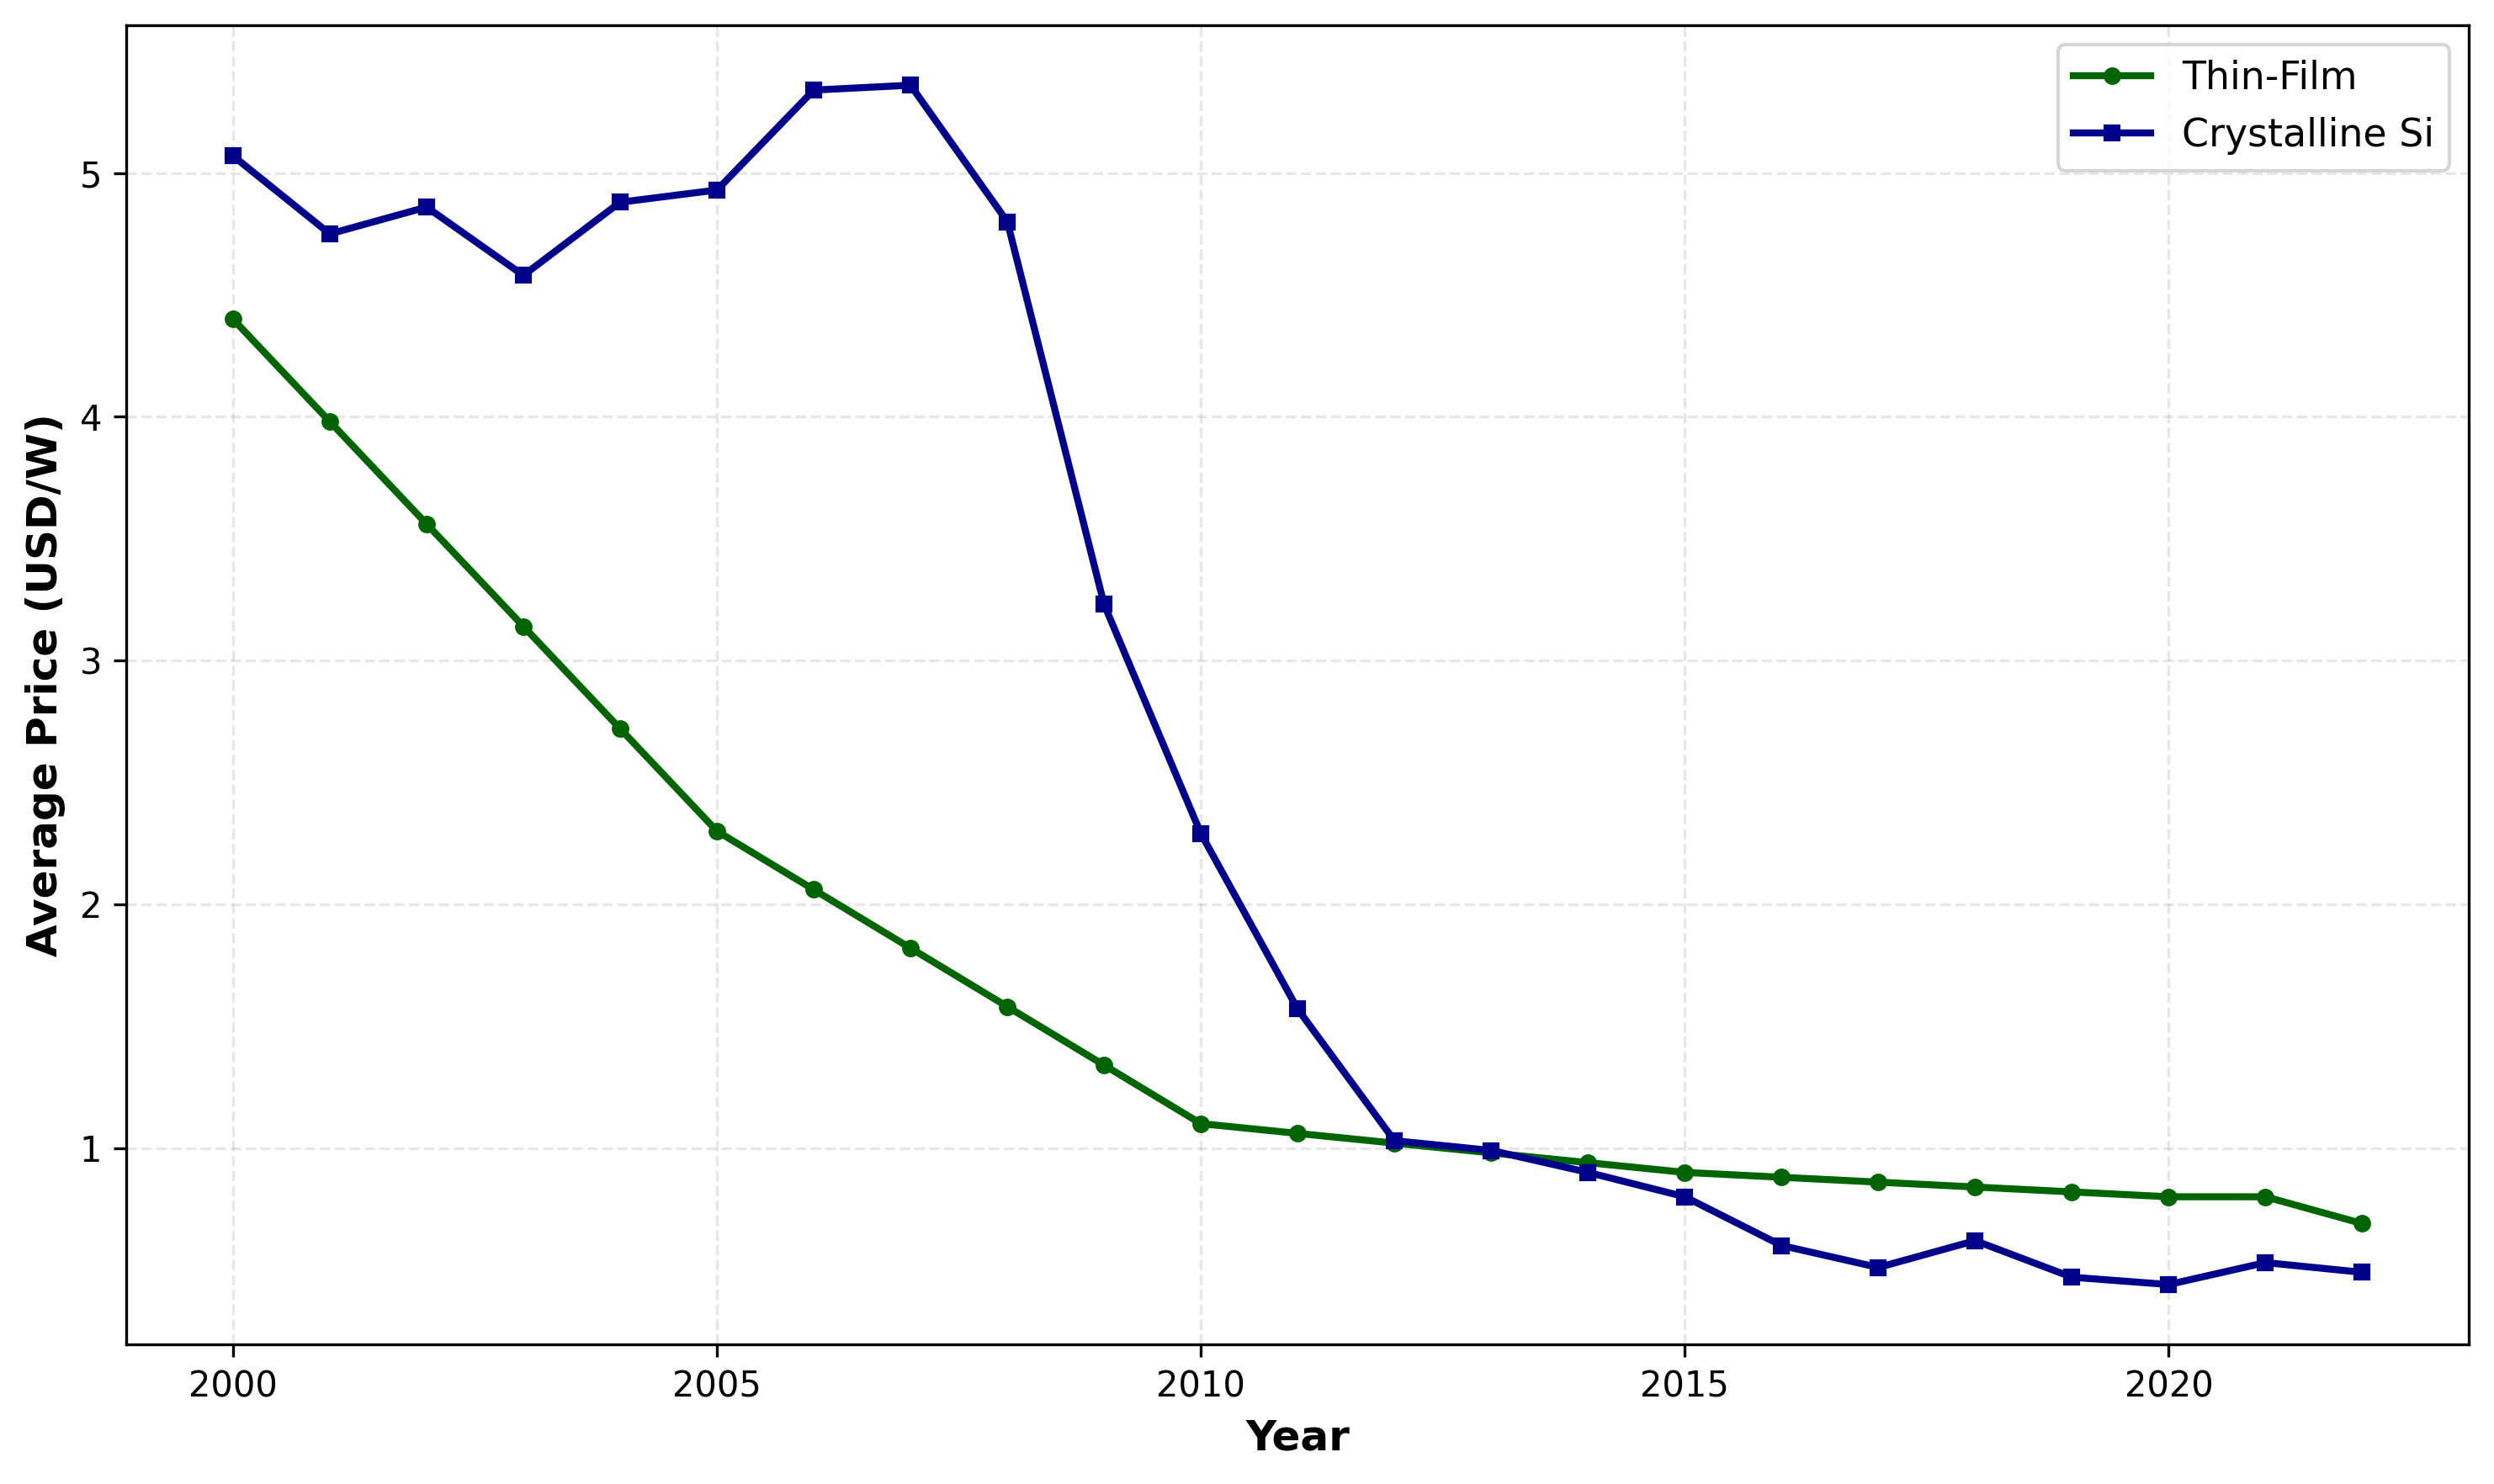
\includegraphics[width=\linewidth]{Figures/price_graph.png}
%         \caption{Price}
%     \end{subfigure}
%     \hspace{0.3cm}
%     \begin{subfigure}[t]{0.5\textwidth}
%         \centering
%         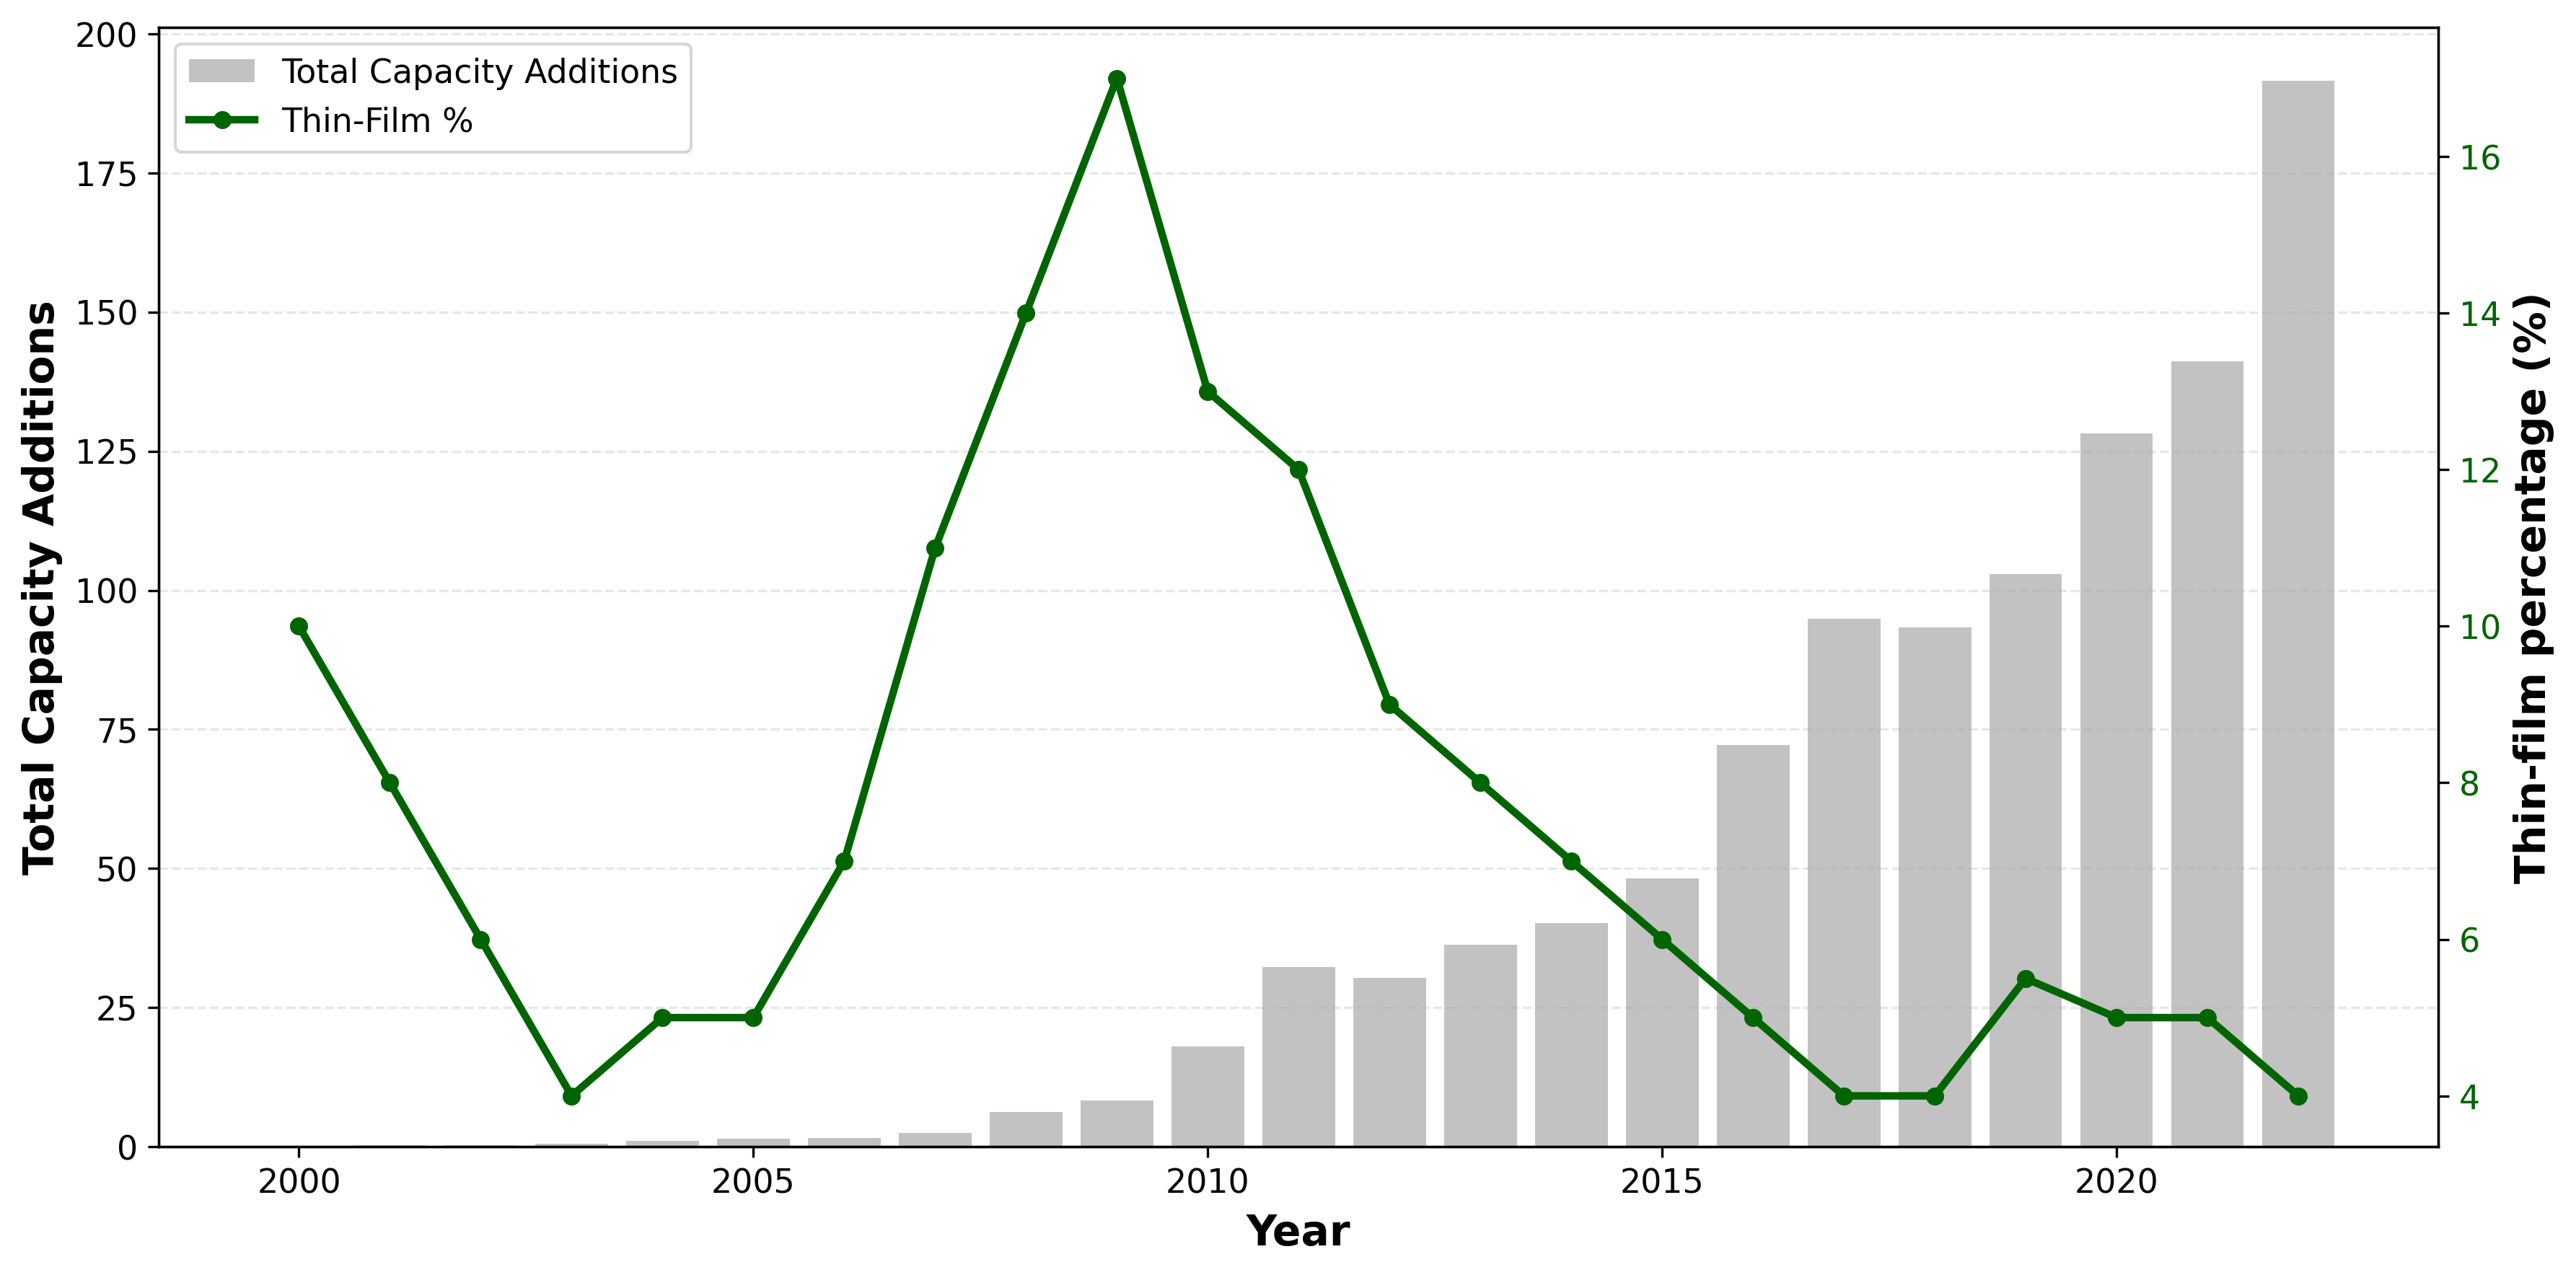
\includegraphics[width=\linewidth]{Figures/capacity_share_graph.png}
%         \caption{Installed Capacity}
%     \end{subfigure}

% \end{figure} 

\begin{figure}[tbh]
\centering
\caption{\label{fig:data_sum_two_tech_price_output}Price and Installed Capacity}
\subfloat[Price]
{\centering
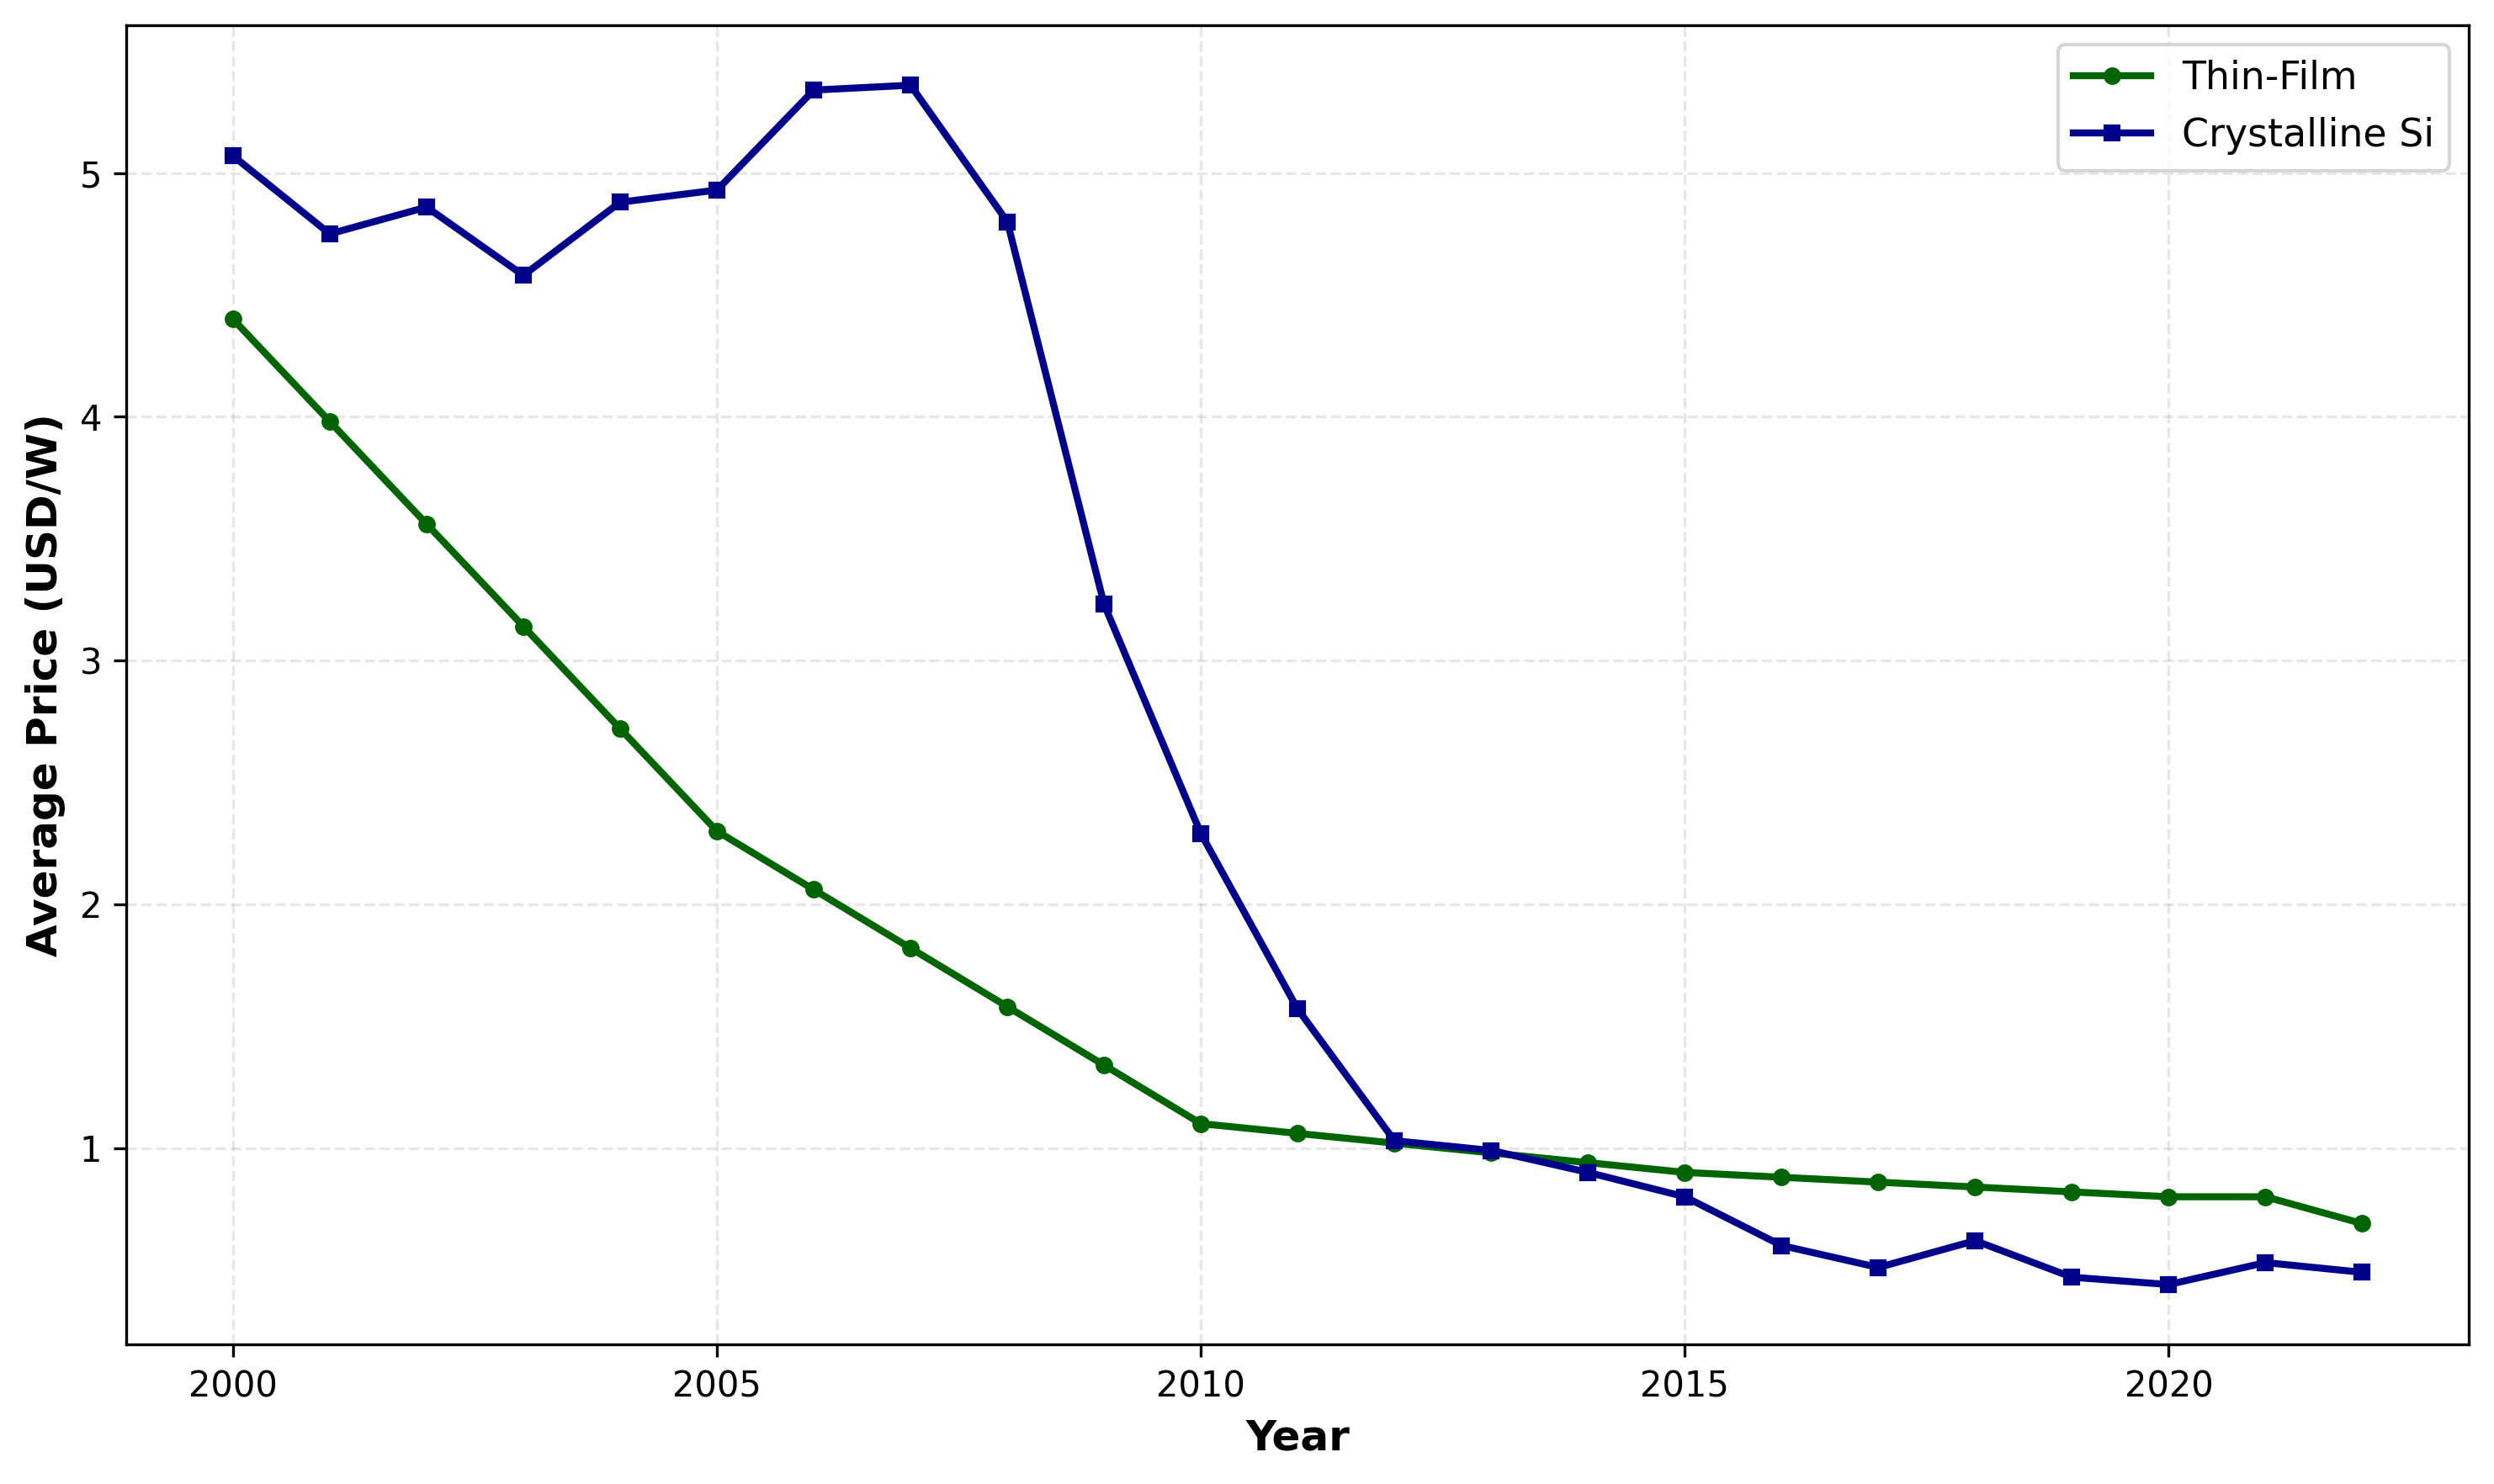
\includegraphics[scale=0.28]{Figures/price_graph.png}
}
\subfloat[Installed Capacity]
{\centering
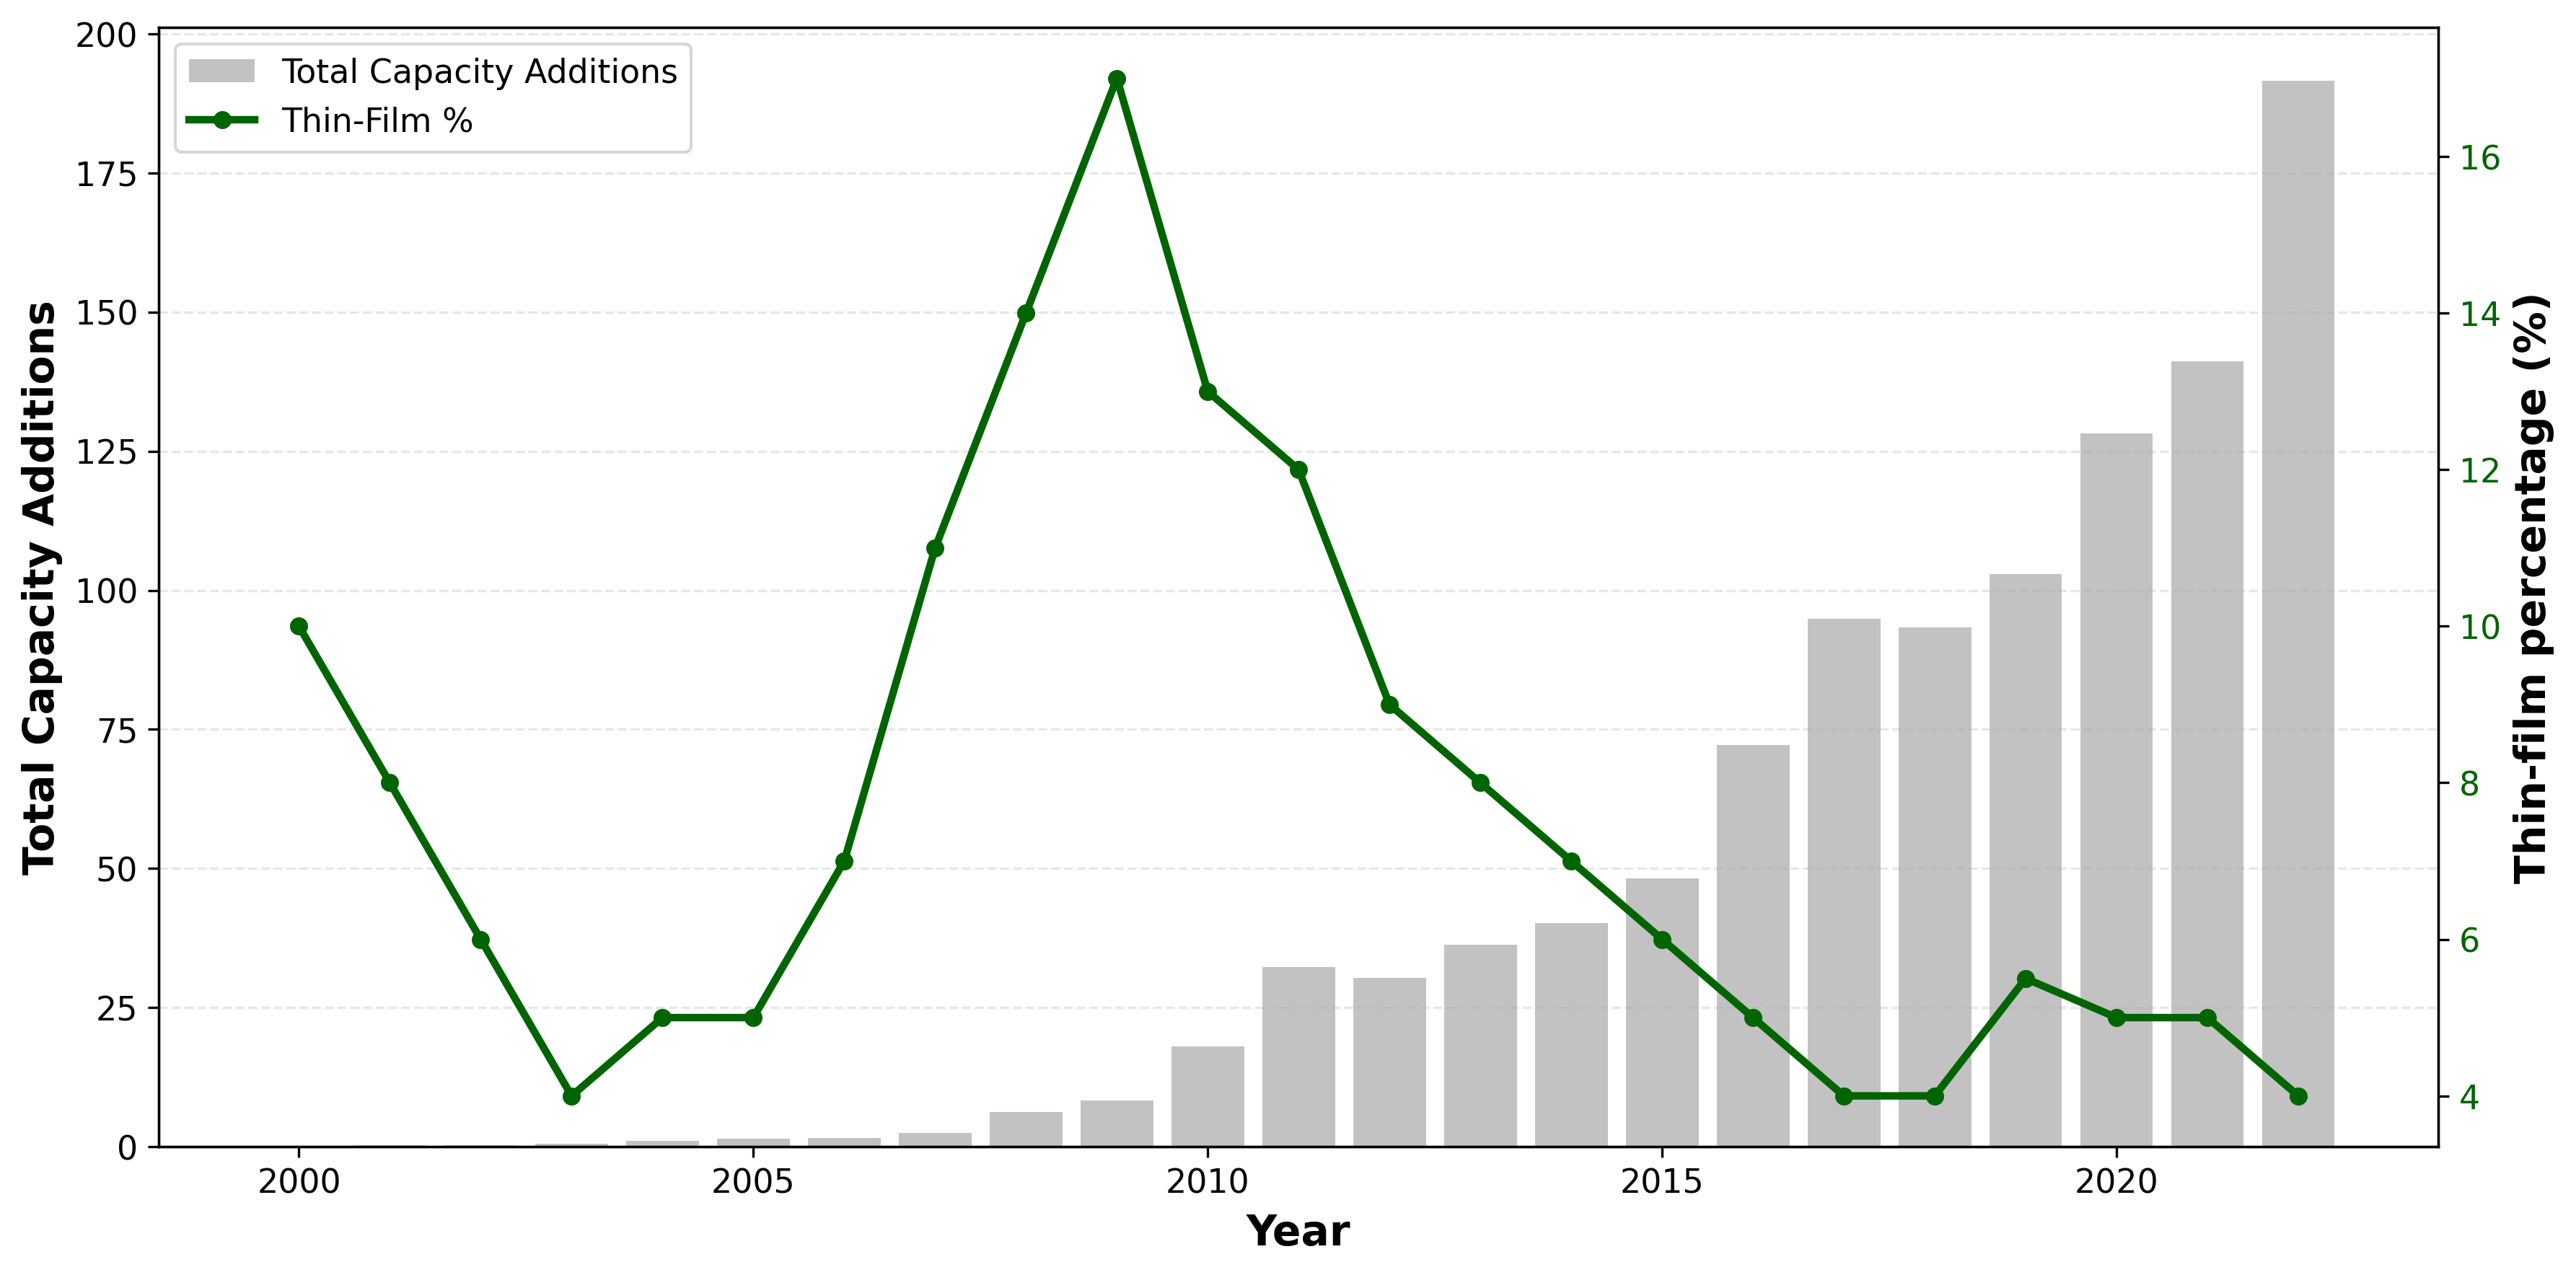
\includegraphics[scale=0.28]{Figures/capacity_share_graph.png}
}
\end{figure}

Noticeably, the price of c-Si solar panels was notably high and even rising before 2008, but it began to drop rapidly after 2008 and has remained low since. A major factor in this trend is the price of polysilicon, the main component of c-Si solar panels, which experienced a sharp increase in late 2007, as shown in Figure \ref{fig:data_sum_two_tech_input_price}(a). This surge was mainly due to the growing demand from the semiconductor sector. 
This situation led to increased investment, which do not depend on polysilicon, and the prices of the primary inputs for this type of solar panels \textcolor{blue}{remained quite stable}, as illustrated in Figure \ref{fig:data_sum_two_tech_input_price}(b).
Meanwhile, it also triggered substantial investments in polysilicon production, primarily in the U.S.. As new production came on line, along with the global recession staring in 2008, the price of polysilicon declined rapidly, falling even below pre-surge levels.  


\begin{figure}[tbh]
\centering
\caption{\label{fig:data_sum_two_tech_input_price}Price of Primary Inputs}
\subfloat[c-Si]
{\centering
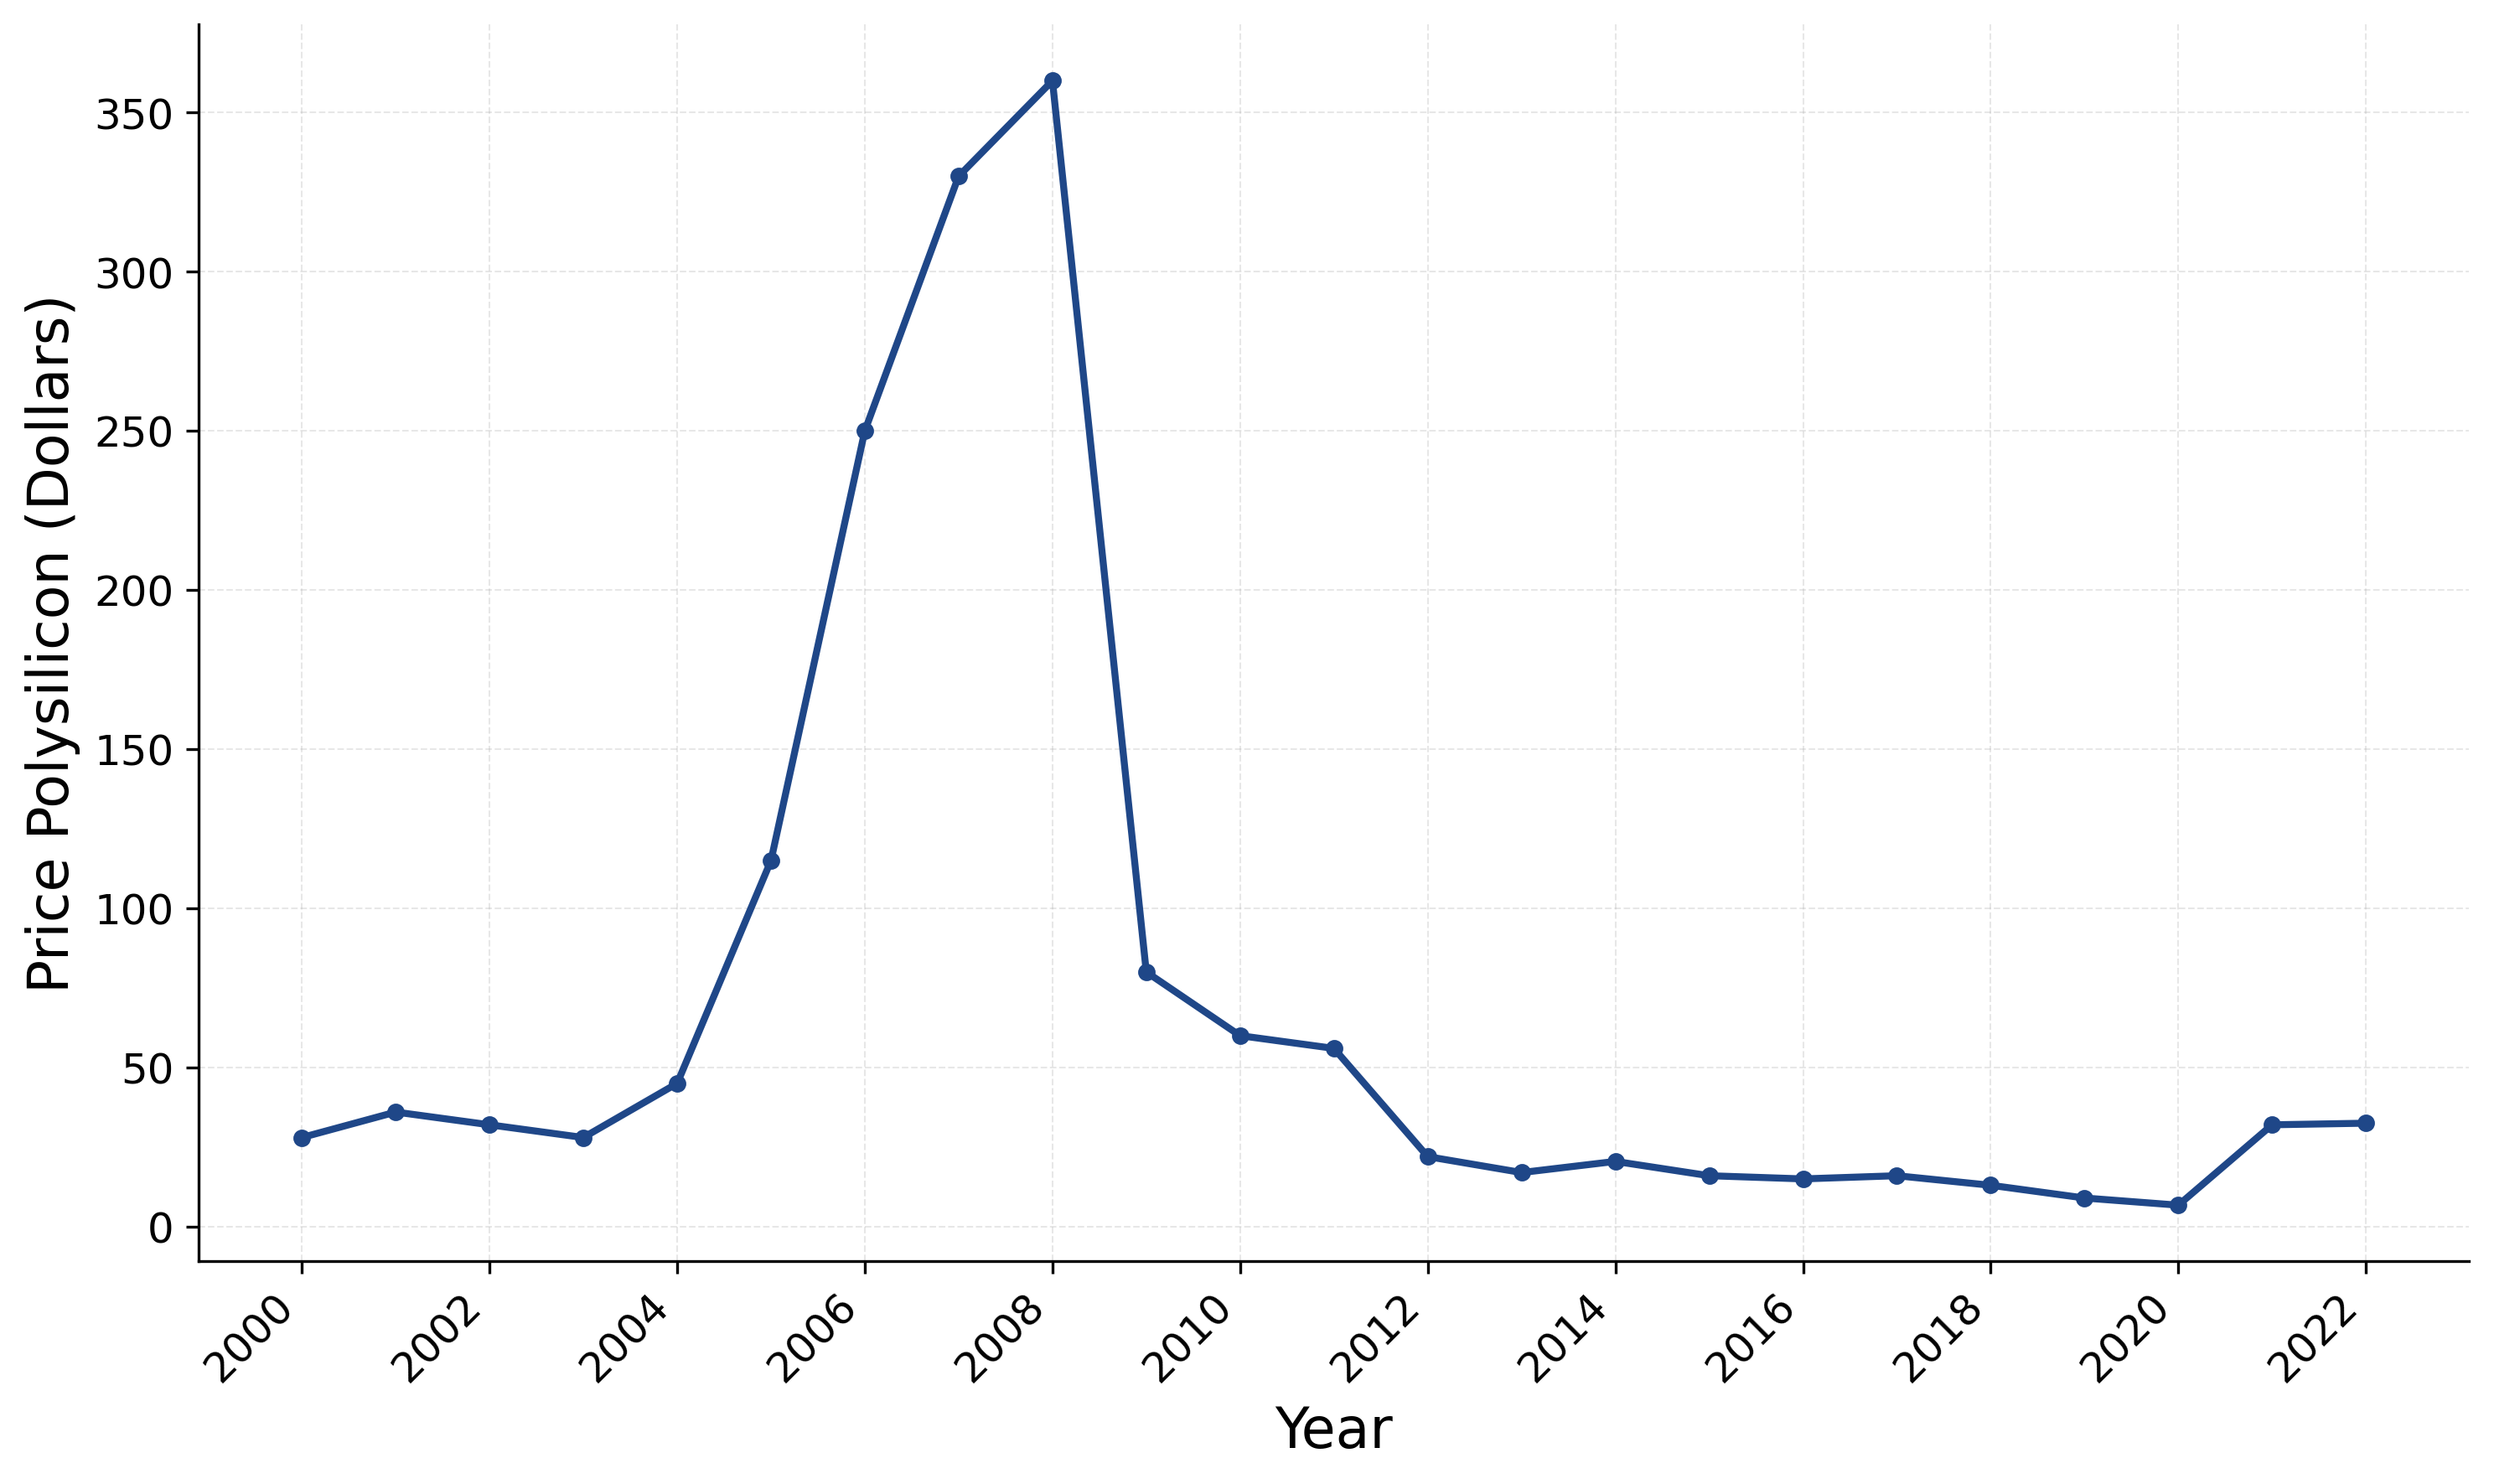
\includegraphics[scale=0.3]{Figures/polysilicon_price_series.png}
}
\subfloat[Thin-Film]
{\centering
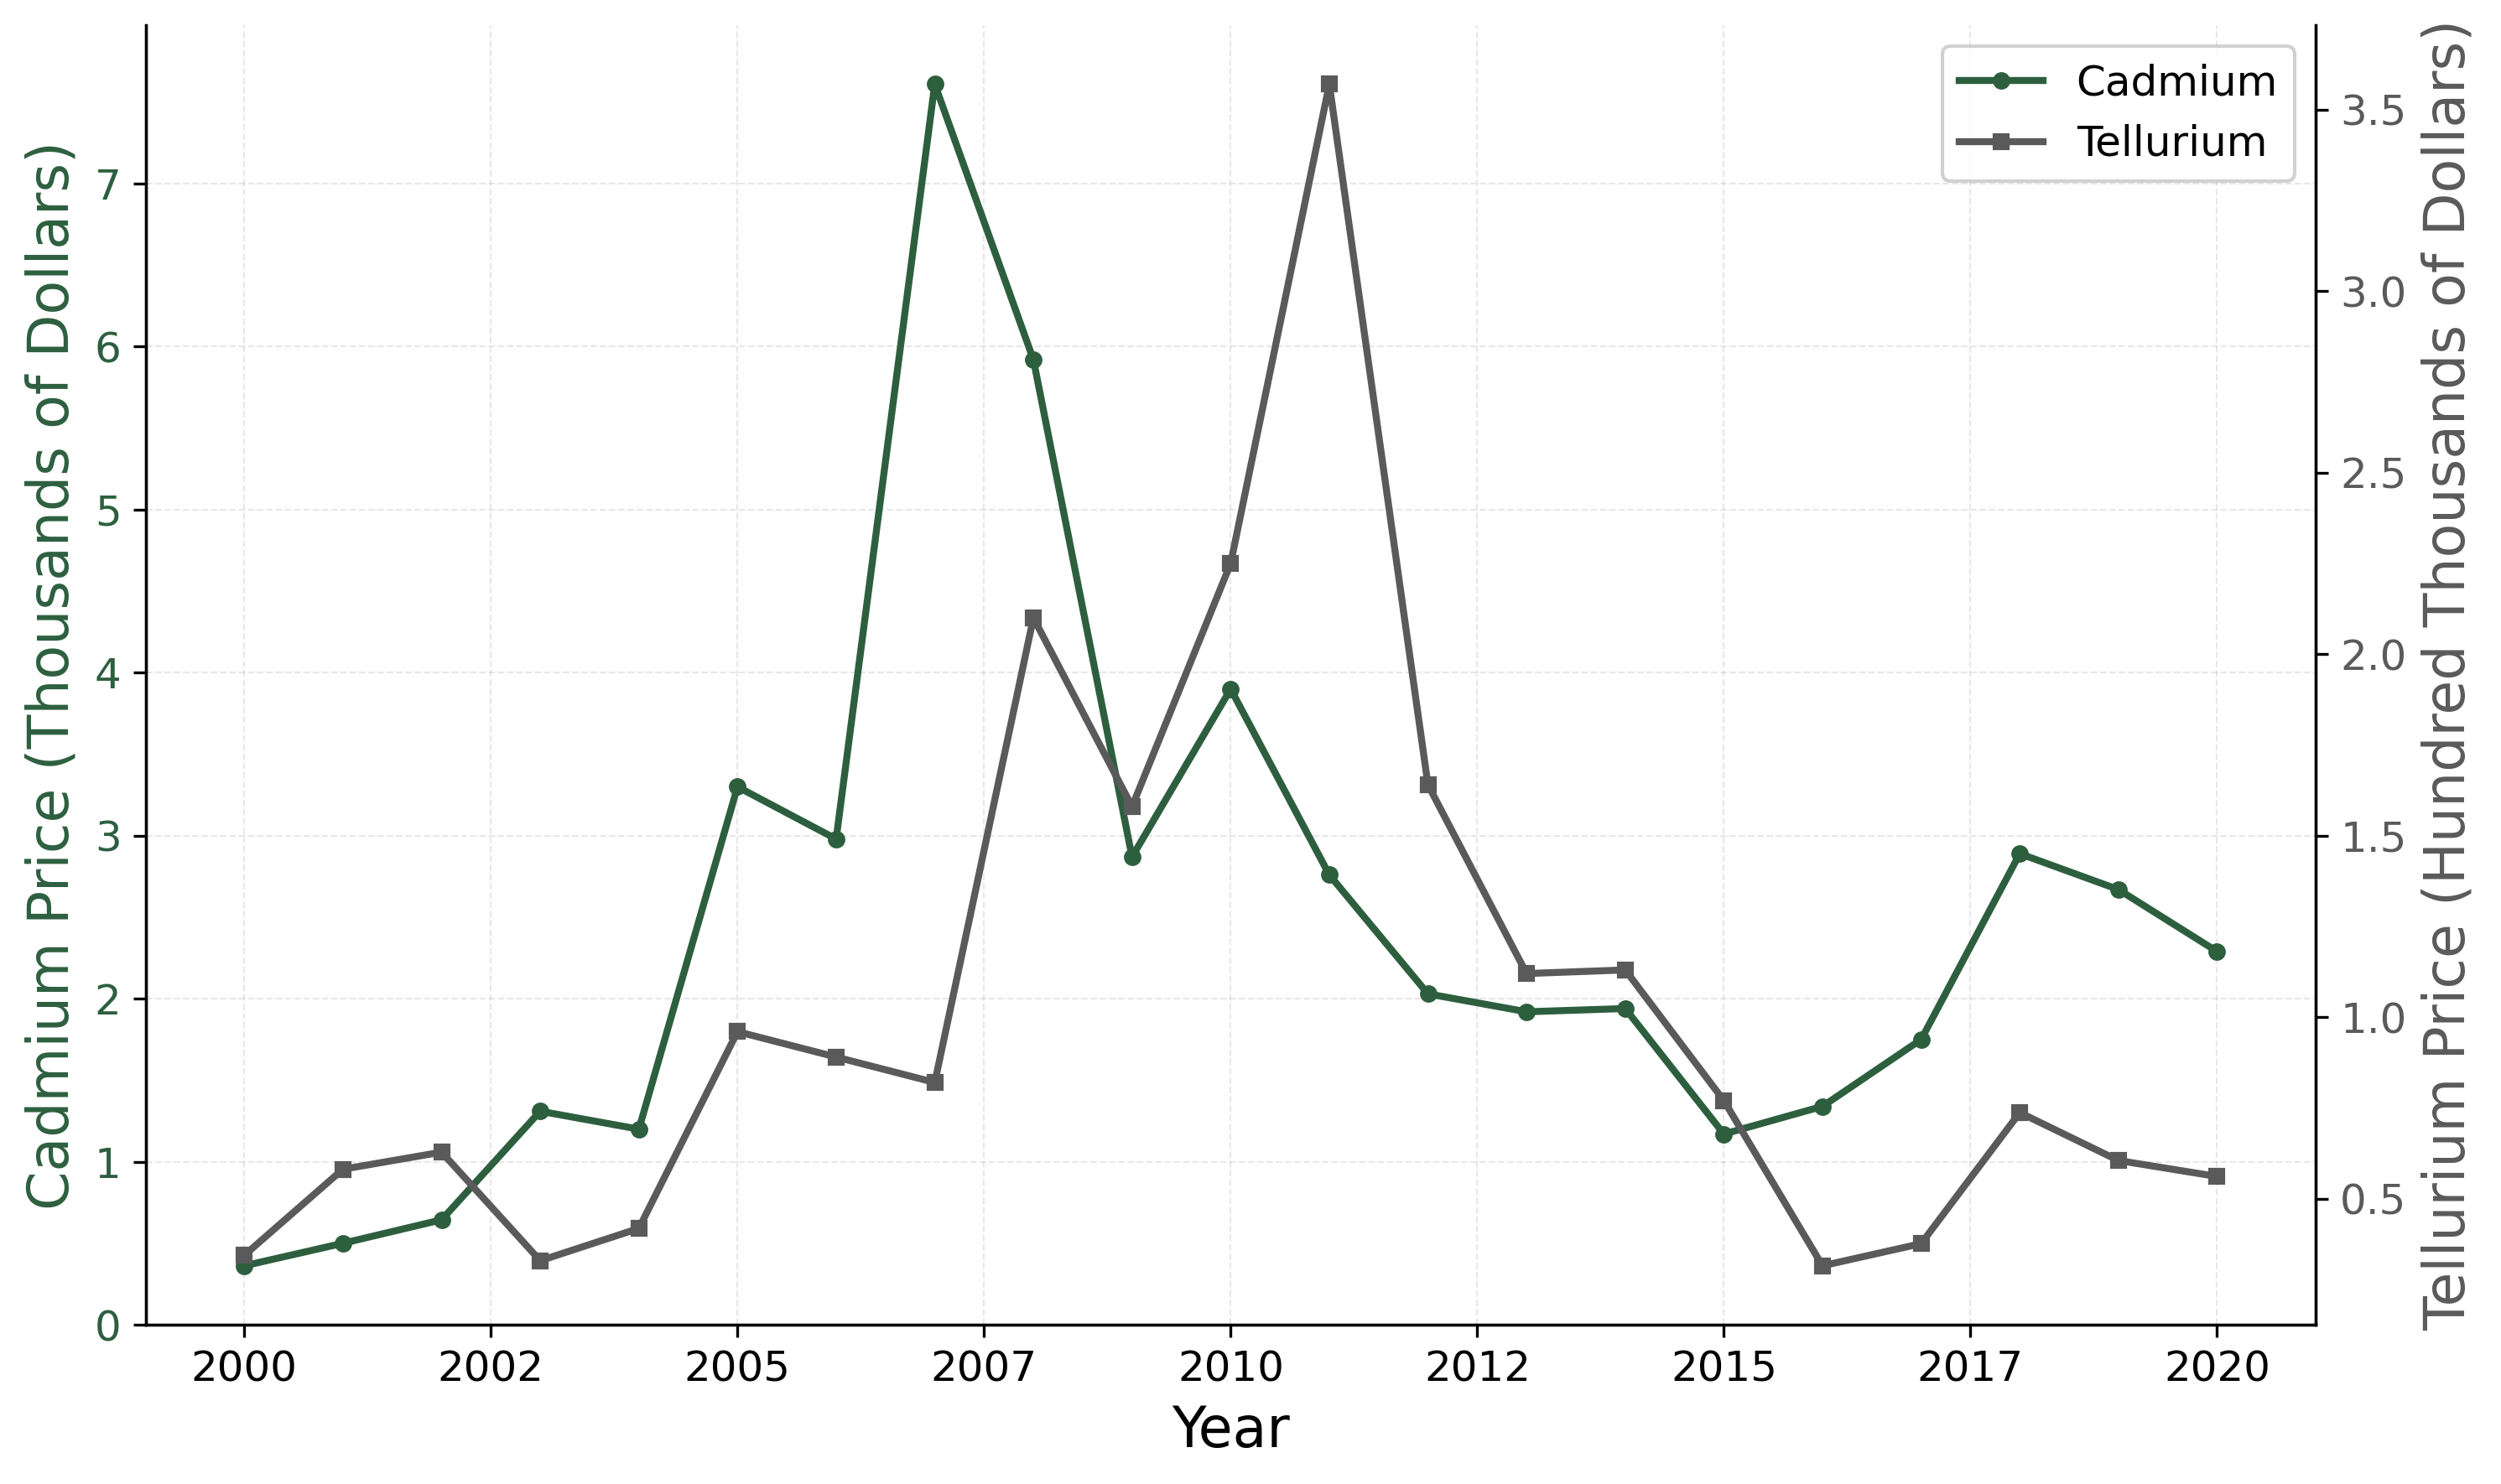
\includegraphics[scale=0.3]{Figures/cadmium_tellurium_prices.png}
}
\end{figure}

\subsection{Industrial Policies}
\label{subsec:ind_policy}
The rapid expansion of solar panel adoption is partly driven by a variety of industrial policies implemented around the world.  These policies fall into two primary categories.  The first consists of demand-side policies, designed either to encourage consumers to install solar panel systems or to discourage the use of certain types of solar panels. The second comprises production-side policies, which directly affect manufacturers' costs related to producing solar panel, as well as entering or exiting the market.

\paragraph{Demand-Side Policies}
Demand-side subsidies to encourage the adoption of solar panels have been implemented worldwide. The most widely used form is feed-in tariffs, in which governments provide a fixed payment for each unit of renewable electricity fed into the grid. These tariff rates differ substantially over time and across countries. A second form of demand subsidy is output-based support, such as net metering. A third common type of subsidy is direct payments or tax credits to cover a proportion of the upfront investment costs. 

The primary form of subsidy in the EU has been feed-in tariffs, in place since the early 2000s. For example, Germany and Spain offered solar feed-in tariffs of 40–60 cents per kWh, far exceeding the wholesale electricity prices received by other forms of electricity generations. By contrast, the primary federal demand-side subsidy in the US is the Investment Tax Credit, which provided a 30\% subsidy on upfront capital costs. In 2009, China launched the ``Golden Sun Program" to speed up the deployment of solar panel power plants, covering up to 50\% of investment costs through 2013, after which it was replaced by other policy instruments.\footnote{Further details on the program can be found in \cite{iea_golden_sun_2021}.} In addition, China implemented feed-in tariffs in 2010, with rates comparable to those offered in the EU.

The rapid decline in solar panel prices has not been without controversy. \citet{nemet2019solar} uses ``gift to the world" to refer to the dramatic production cost reductions achieved by Chinese solar panel manufacturers. However, other nations view China's dominance in solar panel manufacturing as a competitive threat. This perception is partly due to accusations of unfair trade practices and industrial policies by the Chinese government. In response, both the US and the EU have implemented a range of measures aimed at safeguarding their domestic industries since 2010. The first round of anti-dumping and countervailing duties was introduced in 2012. In addition, both the US and the EU start to impose tariffs on c-Si solar panels imported from China. Additional information on US tariffs on solar panels is provided in \citet{bollinger2025strategic}.

 The sharp drop in solar panel prices has generated considerable debate. \citet{nemet2019solar} characterizes the substantial reductions in production costs achieved by Chinese solar manufacturers as a “gift to the world.” Yet many countries regard China’s dominant position in solar panel production as a competitive threat. This concern is fueled in part by allegations of unfair trade practices and government-backed industrial policies in China. In reaction, the US and the EU have, since 2010, adopted various measures to protect their domestic industries. The first wave of anti-dumping and countervailing duties was imposed in 2012. Moreover, both the US and the EU began levying tariffs on c-Si solar panels imported from China. Further details on US tariffs on solar panels can be found in \citet{bollinger2025strategic}.
 
% In response to the surge in Chinese production, both the US and the EU have implemented a range of measures aimed at safeguarding their domestic industries since 2010.  The US enacted the first round of anti-dumping and countervailing duties in 2012. For major Chinese producers who participated in the investigations, the anti-dumping margins ranged from 18.3\% to 31.7\%, while all other Chinese producers were assigned a “PRC-Wide Entity” rate of 249.96\%. In 2014, the US expanded the duties to cover all solar panels assembled in China, irrespective of where the cells were manufactured.\footnote{Under the first Trump administration, the tariff regime was further expanded to include a broader set of countries, with a 30\% tariff imposed on crystalline silicon products from all major solar exporters to the US, pursuant to Section 201 of the Trade Act of 1974. In addition, tariffs of up to 25\% were levied on Chinese imports under Section 301 of the same Act. In 2024, the Biden administration revised and prolonged the Section 201 tariffs through 2026 and raised the ad valorem rate on Section 301 tariffs from 25\% to 50\%.} For comparison, the EU launched its initial round of anti-dumping investigations into Chinese solar manufacturers at roughly the same time as the US and subsequently imposed anti-dumping duties on major cooperating Chinese producers ranging from 27.3\% to 64.9\%, as well as a 53.4\% rate on other “PRC-Wide Entity” producers. In 2018, the EU lifted both the anti-dumping tariffs and the minimum import price requirements applied to Chinese producers.

% They initiated multiple anti-dumping investigations against Chinese manufacturers and imposed tariffs on solar cells manufactured in China.

% The US enacted the first round of US anti-dumping and countervailing duties in 2012. For major Chinese producers who participated in the investigations, the anti-dumping margins ranged from 18.3\% to 31.7\%, while all other Chinese producers were assigned a “PRC-Wide Entity” rate of 249.96\%. In 2014, the US implemented a second round of tariffs to address loopholes in the 2012 measures, expanding the duties to cover all solar panels assembled in China, irrespective of where the cells were manufactured. Under the first Trump administration, the tariff regime was further expanded to include a broader set of countries, with a 30\% tariff imposed on crystalline silicon products from all major solar exporters to the US, pursuant to Section 201 of the Trade Act of 1974. In addition, tariffs of up to 25\% were levied on Chinese imports under Section 301 of the same Act. In 2024, the Biden administration revised and prolonged the Section 201 tariffs through 2026 and raised the ad valorem rate on Section 301 tariffs from 25\% to 50\%.

% The EU launched its initial round of anti-dumping investigations into Chinese solar manufacturers at roughly the same time as the US and subsequently imposed anti-dumping duties on major cooperating Chinese producers ranging from 27.3\% to 64.9\%, as well as a 53.4\% rate on other “PRC-Wide Entity” producers. In 2018, the EU lifted both the anti-dumping tariffs and the minimum import price requirements applied to Chinese producers.

%\textcolor{blue}{[Insert two graphs. Graph (a) displays the weighted average feed-in-tariffs for each region for the years panning from 2000 to 2013. Graph (b) displays the tariff rate imposed by US and EU on Chinese solar panels during this period.]}

\paragraph{Production-Side Policies} Direct subsidies to producers are relatively limited in the EU and the US,\footnote{Some manufacturers have benefited from targeted subsidies, such as R\&D loans or funding to renewable energy.} but are prevalent in many emerging economies, especially in China. 
China supported the solar panel manufacturing industry through an extensive range of policy instruments. During the initial growth phase, most of solar panel production subsidies were granted by provincial and local government. These took the form of reduced land prices or rents, low-interest loans, tax exemptions, and decreased electricity rates.\footnote{For example, Suntech in Jiangsu  benefited from \$3.7 billion in low-interest loans from a state-owned bank and an additional \$1.4 billion in tax rebates and other export support subsidies from 2005 to 2012, as noted in \cite{urban2016solar}.}

During the later stage of the surge, the central government stepped in. In 2010, the State Council declared solar panel as more than just renewable energy, labeling it a ``strategic emerging industry". State-owned banks supported this industry by extending billions of dollars in credits, as mentioned in \cite{lexology2010strategic} and \cite{nahm2023state}. The central government also supported the creation of a domestic silicon industry, although the initial goal was to supply inputs for semiconductors instead of solar panels. According to data from \cite{waferpro_2024_china_silicon_supply}, China's polysilicon production surged from 6,000 Metric Tons in 2000 to 410,000 in 2019. %However, China was still a major importer of polysilicon before 2024, as noted by \cite{solarbe_2024_global_polysilicon}. The subsidization of polysilicon shielded Chinese solar panel manufacturers from the industry shortages that affected other nations, as mentioned in \cite{bernreuter_2020_polysilicon_market_analysis}.

However, systematic data on the quantitative impact of production-side industrial policies is still scarce. Since these policies cannot be directly measured in practice, we follow an indirect strategy: we use detailed firm-level data on production and entry/exit to infer the implied subsidies on production and entry costs by assuming that the observed decisions arise from the equilibrium of a suitably specified model. This methodology has been employed, among others, by \citet{barwick2025industrial} in their analysis of the Chinese shipbuilding industry.


\subsection{Data}
\label{subsec:inst_data}

Our analysis combines data from multiple sources spanning the years 2000 to 2013. 

\paragraph{Chinese Solar Panel Export Volumes}
The first source is the \textit{Chinese Customs Transactions}, which contains the quantity and trade value of all Chinese solar panel export transactions. Using this dataset, we construct export volumes at the firm–destination–year level. For the empirical analysis, we group export destinations into five regions: the EU, India, Japan, the US, and the Rest of the World (ROW).

\paragraph{Chinese Solar Panel Manufacturers}
The second data source is the \textit{Annual Survey of Manufacturing}, an annual survey administered by the Chinese National Bureau of Statistics that provides detailed information on the manufacturing firms surveyed. This dataset has been used in various academic studies, including \citet{roberts2018role} on the footwear industry and \citet{barwick2025industrial} on shipbuilding, among others. \textcolor{blue}{[Some description about how we identify solar panel manufacturing firms.]} For each manufacturer in each year, the survey reports its output, total fixed assets, and a set of time-varying characteristics, such as location (province), ownership status (whether it is state-owned, privately owned, or foreign firm), and the year in which the firm was established.  Using data on total fixed assets, we construct measures of capital stock and investment following the methodology in \citet{brandt2012creative} and \citet{barwick2025industrial}.

\paragraph{Regional-Level Solar Panel Installation and Demand Incentives}
We obtain quarterly information on the solar panel installation for each technology for each of the six economic regions -- China, EU, India, Japan, US, and ROW -- based on data from \cite{OWID_solar_pv_capacity_2025} and \textcolor{blue}{percentages drawn from various news and literature sources cite}. In addition, we collect information on demand subsidy policies in each economic region, including tax credit or rebates, feed-in tariff rates, and import tariff rates on c-Si solar panels. The data on tax credits and rebates and feed-in tariff rates is sourced from \textit{IEA's database} and also \cite{gerarden2023demanding}.

\paragraph{Prices of Solar Panel and Inputs for each Technology}
We obtain the quarterly global price per Watt for each of the two technologies, along with the quarterly global price for Polysilicon and the annual prices for Cadmium, and Tellurium. The quarterly Polysilicon price data is sourced from \textit{Bloomberg New Energy Finance} and \textit{Bernreuter Research}, while the annual prices of Cadmium, Tellurium, silver, and aluminum are obtained from the \textit{United States Geospatial Services (USGS)}. 

\paragraph{Auxiliary Data}
We supplement our main data with several auxiliary data. First, we compile aggregate annual production figures for the two solar panel technologies in regions outside China over the sample period. Second, we collect socioeconomic variables (such as GDP and total electricity consumption) for each economic region. Third, we obtain the global prices for key inputs used in the two solar panel manufacturing technologies, including polysilicon, cadmium, and tellurium.


\subsection{Descriptive Evidence}
\label{subsec:inst_china_PV}

Figure \ref{fig:data_sum_China_output}(a) presents China's production of the two solar panel technologies and its share in the global market.
China's solar panel manufacturing industry was miniscule in the early 2000s. 
The cell production was 3 megawatts (MW) in 2000, accounting for less than 2 percent of global output. China’s share then jumped to 14 percent in 2006 and grew fast over the following five years. By 2011 it reached 60 percent and has remained above that level ever since. The figure also shows that China’s solar panel manufacturing is dominated by c-Si technology, whereas the global share of thin-film fluctuates over time, particularly in response to changes in polysilicon prices, as shown in Figure \ref{fig:data_sum_two_tech_price_output}(b).
%The cell production was 3 megawatts (MW) in 2000 according to \cite{EarthPolicy_indicator12_solar_2000_2013}, accounting for less than 2 percent of global output. It is evident that China’s expansion accelerates after 2005 and is concentrated primarily in c-Si technology.

Figure \ref{fig:data_sum_China_output}(b) displays the number of new entries, exits, and active solar panel firms in China during this time period. It indicates that a massive wave of new solar panel firm entries occurred after China declared solar panel as a ``strategic emerging industry" in 2010. New entries jumped to 118 in 2010 and remained above 50 in subsequent years. At the same time, a comparable volume of firm exits kept the total number of active firms relatively stable at about 200. 

As illustrated in Figure \ref{fig:data_sum_two_tech_price_output}(a), solar panel prices stayed high in the early 2000s, reached a peak in 2007, started to fall after 2008, and remained low from 2011 onward. In contrast, China's production grew steadily before 2009 and then accelerated after 2010, closely aligning with the timing of major industrial policy rollouts.

%China’s solar panel manufacturing industry was miniscule before 2005.  It breached 100 megawatts (MW) of cell production in that year, jumping to 7 percent of global supply from less than 2 percent in 2003. Production grew by an order of magnitude in the next two years, another order of magnitude in the following three, and doubled again in 2011, capping roughly 200x growth in a six-year span. China’s share of the global market had surpassed 60 percent by 2011, and it has remained above that level since then.


\begin{figure}[tbh]
\centering
\caption{\label{fig:data_sum_China_output}China's Market Share and Number of Firms}
\subfloat[Market Share]
{\centering
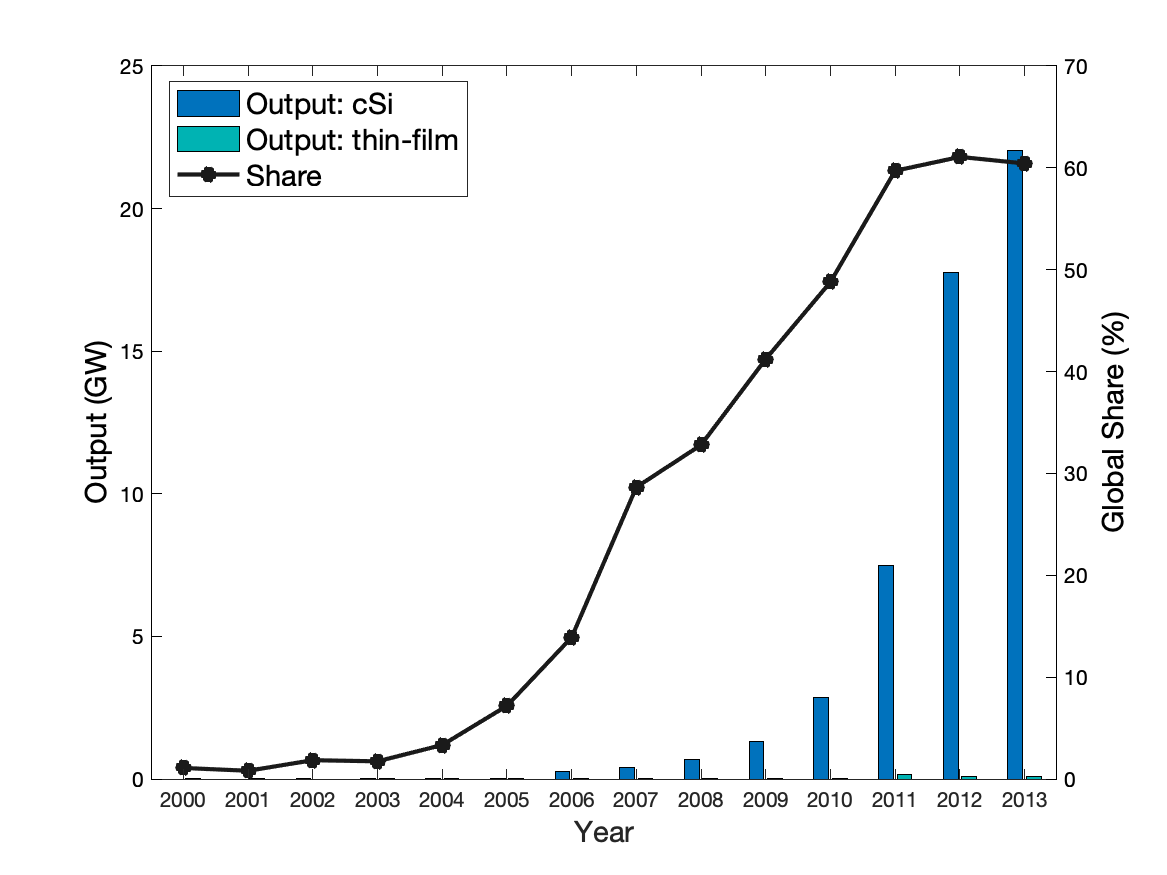
\includegraphics[scale=0.4]{Figures/Fig_data_sum_mkt_share.png}
}
\subfloat[Number of Firms]
{\centering
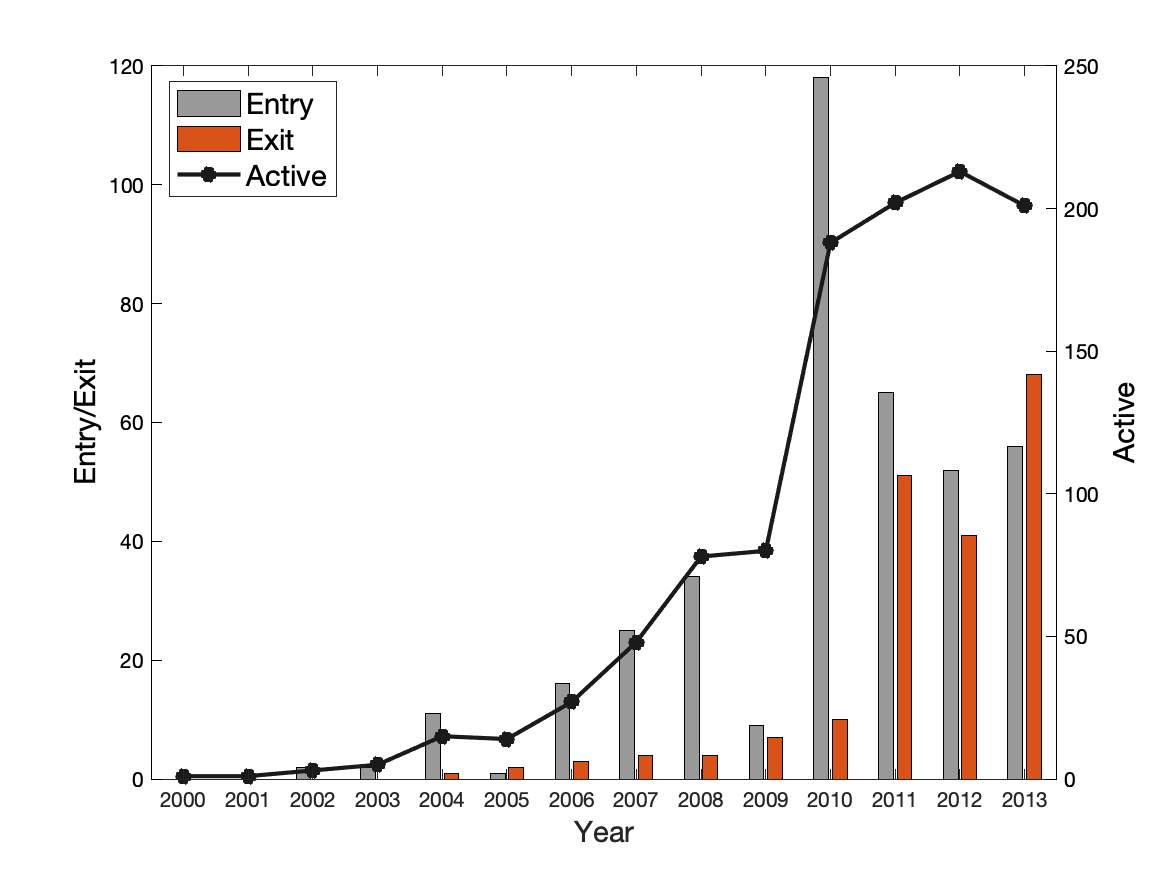
\includegraphics[scale=0.4]{Figures/Fig_data_sum_num_firms.png}
}
\end{figure}


% China supported the solar panel manufacturing industry through an extensive range of policy instruments. During the initial growth phase, most of solar panel production subsidies were granted by provincial and local government. These took the form of reduced land prices or rents, low-interest loans, tax exemptions, and decreased electricity rates. For example, Suntech in Jiangsu  benefited from \$3.7 billion in low-interest loans from a state-owned bank and an additional \$1.4 billion in tax rebates and other export support subsidies from 2005 to 2012, as noted in \cite{urban2016solar}.

% During the later stage of the surge, the central government stepped in. In 2010, the State Council declared solar panel as more than just renewable energy, labeling it a "strategic emerging industry". State-owned banks supported this industry by extending billions of dollars in credits, as mentioned in \cite{lexology2010strategic} and \cite{nahm2023state}. On the demand side, the central government initiated the Golden Sun Project, which provided a subsidy covering up to 70\% of installation costs for developers of off-grid solar panel systems. Additionally, it offered a subsidy for Grid-connected projects with a 300 kW capacity, covering 50\% of the installation and electricity transmission costs. Further details on the program can be found in \cite{iea_golden_sun_2021}.

%The central government also supported the creation of a domestic silicon industry, although the initial goal was to supply inputs for semiconductors instead of solar panels. According to data from \cite{waferpro_2024_china_silicon_supply}, China's polysilicon production surged from 6,000 Metric Tons in 2000 to 410,000 in 2019. However, China was still a major importer of polysilicon before 2024, as noted by \cite{solarbe_2024_global_polysilicon}. The subsidization of polysilicon shielded Chinese solar panel manufacturers from the industry shortages that affected other nations, as mentioned in \cite{bernreuter_2020_polysilicon_market_analysis}.

% The rapid decline in solar panel prices has not been without controversy. \citet{nemet2019solar} uses ``gift to the world" to refer to the dramatic production cost reductions achieved by Chinese solar panel manufacturers. However, other nations view China's dominance in solar panel manufacturing as a competitive threat. This perception is partly due to accusations of unfair trade practices and industrial policies by the Chinese government. In response, to bolster their local manufacturers, both the U.S. and the E.U. have implemented high tariffs on solar imports from China and other nations.\footnote{In June 2022, the Biden administration used the Defense Production Act to accelerate the development of solar panel manufacturing within the country.}

\begin{comment}
Table \ref{tab:data_sum} reports the summary statistics on key variables of interest of Chinese solar panel manufacturers.

\begin{table}[!h]
\centering
\caption{Summary Statistics on Chinese solar panel Manufacturers}
\label{tab:data_sum}
\begin{threeparttable}
\begin{tabularx}{0.7\textwidth}{Xcccccc}
\toprule
Variable & Mean & SD \\
\midrule
\multicolumn{3}{l}{\textit{c-Si solar panel:}} \\
%$\mathds{1}(\text{Polysilicon solar panel})$ &   &  \\
\quad Output (GW) &  65 & 300 \\
%\quad Investment (mill RMB) &  9.32 & 32.90 \\
\quad Capital (mill RMB) & 362  & 881 \\
\quad Age & 5.701  & 5.59 \\
\quad $\mathds{1}(\text{Private owned})$ & .435  & .496 \\
\quad $\mathds{1}(\text{Foreign JV})$ & .516 & .500 \\

\multicolumn{3}{l}{\textit{Thin-film solar panel:}} \\
%$\mathds{1}(\text{Polysilicon solar panel})$ &   &  \\
\quad Output (GW) & 24 & 70\\
%\quad Investment (mill RMB) & 9.59  & 17.1 \\
\quad Capital (mill RMB) & 455  &663  \\
\quad Age &  5.67 & 4.48 \\
\quad $\mathds{1}(\text{Private owned})$ & .112  & .317 \\
\quad $\mathds{1}(\text{Foreign JV})$ & .806  &  .397 \\
\bottomrule
\end{tabularx}
\begin{tablenotes}
  \item  Notes: This table includes 912 firm-year level observations of c-Si solar panel and 98 firm-year level observations of thin-film solar panel.
\end{tablenotes}
\end{threeparttable}
\end{table}
\end{comment}

\section{Model}
In this section, we present a dynamic model of firm entry, technology adoption, exit, and production. Time is discrete and a period is a year, denoted as $t$. There are two types of technologies, with $n=1$ denotes c-Si and $n=2$ denotes thin-film solar panels. The global market is divided into $m=1,...,m$ economic regions, including China, EU, India, Japan, US, and rest of the world (ROW). In any given period, there exist $j = 1,...,J_{nt}$ firms in the world that produce solar panels using technology $n$. 

At the beginning of every period, incumbent firms observe their scrap values and decide whether to exit the market. If they choose to stay, these incumbents observe their production cost shocks for each region and determine how many units to produce for each region. Meanwhile, potential entrants observe their entry shocks and decide on whether to enter and, if they do, choose which technology to adopt. 


% At the beginning of every year $t$, incumbent firms observe scrap value $\phi_{jnt}$ and decide whether to exit. Conditional on remaining active, incumbent firms observe production cost shocks for each region $\omega_{jnmt}$, choose how many units to produce for each region $q_{jnmt}$. Entrants observe entry shock $\zeta_{jnt}$, decide whether to enter and if entering, which technology to use.

\subsection{Per-Period Demand}

The aggregate inverse demand for technology-$n$ solar panel is expressed as:
\begin{equation}
Q_{nmt}=Q_{nm}(P_{1mt},P_{2mt},X_{mt}), \label{eq:model_demand}
\end{equation}
where $Q_{nmt}$ is the total quantity of technology-$n$ solar panel products demanded by consumers in region $m$ during time period $t$. The vector $X_{mt}$ includes various demand shifters, such as overall economic activity indicators, regional fixed effects, and year  fixed effects. The variable $P_{nmt}$ is the price faced by  consumers to install a technology $n$ solar panel system, encompassing both the retail panel  price and installation costs. This consumer price may differ from the global price $P_{nt}$ due to region-technology-specific tariffs and installation subsidies. Specifically, the consumer price is given by:
\[P_{nmt} = P_{nt}\times (1 + \text{tariff}_{nmt}) + P^{I}_{mt} - \text{subsidy}_{mt},\]
where $\text{tariff}_{nmt}$ is the tariff rate, which applies only to c-Si technology, $P^{I}_{mt}$ is the installation costs, and $\text{subsidy}_{mt}$ is the subsidy amount provided by region $m$ in period $t$.

\subsection{Incumbents: Production and Exit}
At the beginning of each period, incumbents observe their private scrap values that are drawn from a technology-specific distribution, and then decide to either exit or continue operations. We denote the scrap value for technology-$n$ incumbent $j$ as $\phi_{jnt}$ and its distribution as $F_{\phi,n}$. If a firm exits, it receives its scrap value. If it remains active, it observes its marginal cost shocks across all regions, denoted as $\mathbf{\omega}_{jnt} =\{\omega_{jnmt}\}_{m=1}^M$. Remaining active, firms engage in Cournot competition while considering how their current output decisions will influence future production costs. They simultaneously decide the quantity of solar panels to produce for each region, $\mathbf{q}_{jnt} = \{q_{jnmt}\}_{m=1}^M$, to maximize their discounted profit, taking as given the production decisions of rival firms. This new output, $\sum_{m=1}^M q_{jnmt}$, is added to the next period's accumulated experience, which in turn affects its future production costs.

\paragraph{Production Cost}
The production cost for firm $j$ using technology $n$, when choosing a vector $\mathbf{q}_{jnt}$, consists of two parts:
\begin{eqnarray}
   TC_{n}(\mathbf{q}_{jnt},s_{jnt},\mathbf{\omega}_{jnt})&=& C_0(\sum_{m=1}^M q_{jnmt}, s_{jnt}) + \sum_{m=1}^M C_m(q_{jnmt},\omega_{jnmt}) \label{eq:model_c_q},
\end{eqnarray}
where the first component, $C_0(\sum_{m=1}^M q_{jnmt}, s_{jnt})$, represents the total production cost of $\sum_{m=1}^M q_{jnmt}$, which depends on a vector of state variables $s_{jnt}$. These state variables include the firm's accumulated experience $e_{jnt}$, and firm characteristics such as capital, age, location, ownership status, as well as aggregate cost shifters affecting all firms (e.g., input price), and policy dummies that reflect the impact of industrial policies on production costs, including indicators for specific time periods and provinces. The second component, $C_m(q_{jnmt},\omega_{jnmt})$, accounts for the additional cost of transporting $q_{jnmt}$ to region $m$ in year $t$.

The experience of firm $j$, denoted as $e_{jnt}$, can potentially reduces production costs in the future, incentivizing the firm to increase output to gain more experience in the current period.  This experience is defined as the cumulative past production:
\[e_{jnt} = \sum_{\tau<t} \sum_m q_{jnm\tau},\]
where $q_{jnm\tau}$ is the units sold by firm $j$ to region $m$ during year $\tau$. The primary parameter of interest is the learning coefficient, which indicates how rapidly the unit cost of solar panel manufacturing declines as the production experience grows. 

\paragraph{Incumbent Value Function}
The value function of a technology-$n$ incumbent $j$, after observing the scrap value $\phi_{jnt}$ but before observing the realization of the production cost shock $\mathbf{\omega}_{jnt}$, is defined as:
\begin{eqnarray}
V_n(s_{jnt},\phi_{jnt})&=&\max\{\phi_{jnt},CV_n(s_{jnt})\},  \label{eq:incumbent_value_fn} 
\end{eqnarray}
where the continuation value $CV_n(s_{jnt})$  is expressed as:
\begin{eqnarray}
CV_n(s_{jnt}) & \equiv & \mathbb{E}_{\omega}\Big[ max_{\mathbf{q}} \{\sum_m P_{nm}(q_{m}, \mathbf{q}_{-mt},X_{mt}) q_{m} - TC_{n}(\mathbf{q},s_{jnt},\mathbf{\omega}_{jnt})  \nonumber \\
&& +\beta \mathbb{E}[V_n(s_{jnt+1})|s_{jnt}, \mathbf{q}] \}\Big]. \label{eq:incumbent_EV_fn}
\end{eqnarray}
Here, $\mathbf{q} = \{q_m\}_{m=1}^M$ is a vector of output choice for each region, while $\mathbf{q}_{-mt}$ denotes the output vectors that are chosen by other competing solar panel firms for region $m$. The expected value $\mathbb{E}_{\omega}$ is calculated with respect to the production cost shocks $\mathbf{\omega}_{jnt}$, 

\paragraph{Optimal Exit Decision}
The optimal decision to exit follows a threshold structure. A firm exits the market if the scrap value exceeds the continuation value; otherwise, it remains active. Therefore, the probability of exiting is:
\begin{eqnarray}
    p_n^x(s_{jnt}) & \equiv & Pr(\phi_{jnt} > CV_n(s_{jnt})) = 1-F_{\phi,n}(CV_n(s_{jnt})). \label{eq:exit_policy_fn}
\end{eqnarray}

\paragraph{Optimal Production Decision}
Provided that firm $j$ with technology-$n$ stays active, the optimal output level, $q_{jnmt}^*=q_{nm}^*(s_{jnt},\omega_{jnmt})$, satisfies the following first-order condition:
 \begin{eqnarray}
 \frac{\partial TC_{n}(\mathbf{q}_{jnt}^*,s_{jnt},\mathbf{\omega}_{jnt})}{\partial q_{jnmt}^*} & = & \underbrace{
    P_{nmt}+q_{jnmt}^*\frac{\partial P_{nm}(q^*_{jnmt}, \mathbf{q}^*_{-mt},X_{mt})}{\partial q_{jnmt}}}_{\text{Impact on current profit}} \nonumber \\
    && +  \underbrace{\beta \frac{\partial \mathbb{E}[V_n(s_{jnt+1})|s_{jnt}, \mathbf{q}_{jnt}^*] }{\partial q_{jnmt}} }_{\text{Impact on future profits via LBD}}, \label{eq:model_foc_q}
\end{eqnarray}  
where $\mathbf{q}^*_{-mt}$ is a vector of equilibrium outputs that are chosen by all other competing solar panel firms for region $m$ during year $t$.

\begin{comment}
\paragraph{Firm Profit}
Firm $j$'s expected profit before the production cost shocks are realized is given by:
\[
\pi_n(s_{jnt}) = \mathbb{E} [\sum_m \pi_{nm}(s_{jnt},\omega_{jnmt})]
\]
where $\pi_{nm}(s_{jnt},\omega_{jnmt})$ is firm $j$'s equilibrium profit from region $m$.
\end{comment}

\paragraph{Equilibrium Global Price}
In each period, the global price of technology-$n$ solar panels, denoted as $P_{nt}$, equates the aggregate demand and supply, where the aggregate demand is described by equation (\ref{eq:model_demand}) and the aggregate supply is the sum of $q_{jnmt}^*$ defined in equation (\ref{eq:model_foc_q}) across all firms using technology $n$.  
%\textcolor{blue}{We only have data on the Chinese firms, rather than all firms in the world. It is biased to use a subset of firms to compute the global price that equalizes the total supply and total demand.}

\subsection{Potential Entrants: Entry and Technology Selection}
At the end of each period $t$, a total of $\bar N$ potential entrants observe their profit shocks $\zeta_{j0t}$ for not entering, as well as entry costs $\kappa_1(s_{jnt})-\zeta_{j1t}$ for entering with c-Si technology, and $\kappa_2(s_{jnt})-\zeta_{j2t}$ for entering with thin film technology. The terms $\kappa_1(s_{jnt})$ and $\kappa_2(s_{jnt})$ denote the expected entry costs associated with the two technologies. The vector $s_{jnt}$ includes policy dummies to capture the impact of industrial policies on the decisions regarding entry and technology selection.

Upon observing their profit shocks $\zeta$'s, potential entrants make a decision about entering the market and, if they choose to enter, select a technology. Should they decide to enter, they incur the entry cost during the current period and start earning profit from the product market starting from the following period. Therefore, the potential entrant $j$'s maximization problem can be formulated as:
\begin{eqnarray}
 && max\{\zeta_{j0t}, max_{n\in \{1,2\}} \{-\kappa_n(s_{jnt}) + \zeta_{jnt} + \beta \mathbb{E}[V_n(s_{jnt+1}) \mid s_{jnt}]\}\} \}
\end{eqnarray}

A firm stays out of the market if its profit shock from not entering exceeds the expected profit of entering with either technology option. It chooses to enter with technology $n$ if this option provides the highest profit. We use $p^{e,n}(s_{jnt})$ to denote the probability that a potential entrant $j$ enters with technology $n$, given by
\begin{eqnarray}
  p^{e,n}(s_{jnt}) & \equiv & \text{Pr}\{\zeta_{jnt} - \zeta_{jn't}  > \kappa_n(s_{jnt})-\kappa_{n'}(s_{jn't}) + \beta \mathbb{E}[V_{n'}(s_{jn't+1}) \mid s_{jn't}] - \beta \mathbb{E}[V_n(s_{jnt+1}) \mid s_{jnt}] \nonumber \\
  & & \quad  \& \  \zeta_{jnt}-\zeta_{j0t} + >\kappa_n(s_{jnt})-\beta \mathbb{E}[V_n(s_{jnt+1}) \mid s_{jnt}] \} \label{eq:entry_policy_fn}
\end{eqnarray}

\subsection{Markov-Perfect Equilibrium}
A Markov-Perfect Equilibrium is characterized by policy function, $q^*_{nm}(s_{jnt}$,$\omega_{jnmt})$, $p_n^x(s_{jnt})$, $p_n^e(s_{jnt})$, value function $V_n(s_{jnt})$, and global price $P_{nt}$, such that production policy function $q^*_{nm}(s_{jnt},\omega_{jnt})$ satisfies (\ref{eq:model_foc_q}), exit policy function $p_n^x(s_{jnt})$ satisfies (\ref{eq:exit_policy_fn}), entry policy function $p_n^e(s_{jnt})$ satisfies (\ref{eq:entry_policy_fn}), global price $P_{nt}$ ensures that aggregate demand and aggregate supply are in balance, while the incumbent's value function $V_n(s_{jnt})$ satisfies (\ref{eq:incumbent_value_fn}).

\subsection{Discussion of Model Assumptions}

Before moving on to the estimation, we discuss two key simplifying assumptions made by our model. 
%First, we assume that solar panels are homogeneous conditional on their production technology. This assumption is consistent with the highly commoditized nature of solar panels. In addition, \cite{bollinger2025strategic} analyze a dataset of solar panel shipments to the United States, constructed from quarterly IHS Markit data, and document very little price dispersion across manufacturers at any given time.
First, cost shocks $\omega_{jnmt}$ are assumed to be i.i.d., because allowing for a persistent time-varying unobserved state variable in a dynamic model would introduce substantial computational complexity. Nonetheless, our model does incorporate persistent effects through the accumulation of experience. When firms receive positive demand shocks, they increase quantity, which in turn increases their stock of experience.  Since experience is a state variable, firms with more experience have lower production costs and thus choose higher output levels, further building experience and reducing long-run costs. This feedback mechanism is the key driver of why firms that are ex-ante identical can exhibit divergent growth paths over time.

Second, following most of the existing literature such as \citet{ryan2012costs} and \citet{barwick2025industrial}, we assume that all firms view government policies as permanent.  Relaxing this assumption would require modeling firms’ expectations and their adjustment to a changing policy environment, which would greatly increase the complexity of our analysis. This is an important avenue for future research; see \citet{gowrisankaran2025policy} and \citet{chen2024dynamic} for further discussion.


\section{Estimation Strategy}
In this section, we outline the strategy for estimating model parameters. In Section \ref{subsec:est_specifications}, we detail our demand model, specify the production cost function, as well as the distributions related to the scrap value and entry costs. In sections \ref{subsec:est_dynamic_first} and \ref{subsec:est_dynamic_second}, we present the two-stage procedure for estimating dynamic parameters, including those associated with the production cost function and the distributions for the scrap value and entry cost shocks.


% The model contains four primitives: (i) the global demand function for solar panel for each technology and region, $Q_{jnmt}(\cdot)$, (ii) the total production cost function for each technology and region, $TC_{n}(\cdot)$, (iii) the distribution of scrap value, and (iv) the distribution of entry costs for each technology.

%In Section \ref{subsec:est_static} we describe the estimation of the static parameters, which include those associated with the demand functions.  

We estimate the dynamic parameters using the firms' observed choices of production, exit, and entry, including not entering, entering with c-Si technology, or entering with thin-film technology. Using the BBL approach from \citet{bajari2007estimating}, we estimate these parameters in two stages. In the first stage, we flexibly estimate policy functions, including production, exit, and entry with technology selection, as well as the transition process of state variables directly from the data. After that, we approximate the value function using a set of B-spline basis functions of state variables, as described in (\citet{sweeting2013dynamic}). In the second stage, we estimate the dynamic parameters. We provide additional details in Appendix \textcolor{red}{XX}.

\subsection{Specifications}
\label{subsec:est_specifications}

\paragraph{Logit Demand.}
We parameterize the solar panel demand, expressed in (\ref{eq:model_demand}), using a simple Logit model. To be specific, the demand of technology-$n$ solar panels in the region $m$ during the year $t$ is given by:
\begin{eqnarray*}
Q_{nmt} & = & \frac{M_{mt}\cdot exp(-\alpha_{m} P_{nmt} + X_{mt}\eta +\xi_{nmt})}{1+\sum_{n'}exp(-\alpha_{m} P_{n'mt} + X_{mt}\eta +\xi_{n'mt})}.  \label{eq:demand_specification}
\end{eqnarray*}
Here, $M_{mt}$ is the market size for region $m$ in year $t$, measured by the total electricity consumption. $P_{nmt}$ is the price of technology-$n$ solar panels that is faced by consumers in region $m$, calculated by adjusting the global price $P_{nt}$ with local installation cost, tariffs, and subsidies. $X_{mt}$ is a vector of demand shifters, including GPD, feed-in tariff, regional fixed effects, and yearly fixed effects. 

For the given demand, the estimation equation is represented as:
\begin{eqnarray}
ln( \frac{Q_{nmt}}{M_{mt}} ) - ln( \frac{M_{mt}- Q_{1mt}- Q_{2mt}}{M_{mt}} ) & = &  -\alpha_{m} P_{nmt} + X_{mt}\eta +\xi_{nmt}. \label{eq:demand_est_mkt}
\end{eqnarray}

To address the issue of price endogeneity, we follow \citet{bollinger2025strategic} and use the prices of silver and aluminum as instruments for the solar panel price. Silver and aluminum are key inputs in both c-Si and thin-film solar technologies. Our identifying assumption is that the prices and production levels of these two inputs are not correlated with the  regional demand shocks for solar panels, $\xi_{nmt}$. This assumption is plausible because the solar industry represents less than 5\% of global demand for silver and aluminum throughout the sample period, and the share of demand for solar panels originating from any given region is below 1\% of total demand.

% To address the issue of price endogeneity, we use the price and production data of major inputs as instruments. Specifically, we use the global price and output of polysilicon as instruments for the price of c-Si solar panel, and the global prices and outputs of cadmium and tellurium as instruments for the price of thin film solar panel. The assumption for identification is that the global price and output of the inputs are not correlated with the demand shocks for solar panel at the region level, $\epsilon_{nmt}$. \textcolor{blue}{[Are these valid IVs??]}

%This is plausible for the following reasons. First, only a modest portion of global polysilicon production is used in solar panel production during this period, while the major demanders of polysilicon are the semiconductor manufacturing. \textcolor{red}{I am not sure we can make this argument. According to Bernreuter Research, 90 percent of polysilicon was used for solar panels at the end of the period. https://www.bernreuter.com/polysilicon/uses/.} Second, cadmium and tellurium are the by products of steel production, and the proportion of cadmium and tellurium is used in the thin-film solar panel production is negligible. \textcolor{red}{I'm also not sure we can make this argument. USGS considers thin-film solar as a major market for Cadmium https://www.usgs.gov/centers/national-minerals-information-center/cadmium-statistics-and-information. USGS also cites thin-film solar as the primary market for tellurium: https://pubs.usgs.gov/periodicals/mcs2024/mcs2024-tellurium.pdf} Lastly, the demand shock $\epsilon_{nmt}$ is at the region level. It is less of a concern that the demand shock for solar panel in a specific region is correlated with the global price of those major inputs.

\paragraph{Production Costs.} 
%We decompose a firm's cost shock into two components: one capturing the firm's overall efficiency shock $\bar{\omega}_{jnt}$ and the other one capturing the firm's shock in a specific region $\tilde{\omega}_{jnmt}$, that is $\omega_{jnmt} = \bar{\omega}_{jnt} + \tilde{\omega}_{jnmt}$.
As shown in \ref{eq:model_c_q}, the production cost function for firm $j$ of technology-$n$ is decomposed into two components, specified as
\begin{eqnarray*}
   C_0(\sum_m q_{jnmt},s_{jnt}) &=& (\gamma_{n}^0 + s_{jnt} \gamma_n^s) \cdot (\sum_m q_{jnmt}),
\end{eqnarray*}
and
\begin{eqnarray*}
   C_m(q_{jnmt},\omega_{jnmt}) &=& (\gamma_{m}^{ex}+\omega_{jnmt}) \cdot q_{jnmt},
\end{eqnarray*}
where $\gamma_{n}^0$ are technology-specific constants, parameters $\gamma_n^s$ measure the impact of state variables on the unit cost for a specific technology, $\gamma_{m}^{ex}$ are parameters particular to each region that capture the additional cost associated with shipping or exporting to that particular region, and $\omega_{jnmt}$ are cost shocks, which are assumed to follow an independent and identically distributed normal distribution with a mean of zero and a variance of $\sigma_\omega^2$.

As a result, the marginal cost that firm $j$ ships $q_{jnmt}$ to region $m$ is:
\begin{eqnarray}
  \frac{\partial TC_{jnt}}{\partial q_{jnmt}} &=&  \gamma_{n}^0 + s_{jnt} \gamma_n^s  +\gamma_{m}^{ex} +\omega_{jnmt}. \label{eq:est_mc_q}
\end{eqnarray}
Here, the vector of state variables $s_{jnt}$ includes the firm's cumulative experience $e_{jnt}$, along with other firm characteristics such as age, location, and ownership type. In addition, it includes technology-specific cost shifters that impact all firms, such as prices of major inputs, and policy variables that reflect the impact of industrial policies on production costs. As mentioned in Section \ref{subsec:inst_china_PV}, the central government has been directly supporting this industry \textcolor{blue}{since 2009}, and several provincial governments also provide generous support. To capture these policy impacts, we incorporate indicators for the year 2009 onward and for the Zhejiang province. 


\paragraph{Distributions of Scrap Value and Entry Costs.} 
We assume that the scrap value $\phi_{jnt}$ follows an exponential distribution characterized by a parameter $1/\sigma_{\phi}$. \textcolor{blue}{(Note: we can allow the parameter to differ across the two technologies, $1/\sigma_{\phi,n}$)}.
Additionally, we assume that the entry cost shocks $\zeta$ conform to an independent and identically distributed Type 1 Extreme Value (T1EV) distribution.

\subsection{First Stage: Policy Functions and State Transition}
\label{subsec:est_dynamic_first}

\paragraph{Exit Policy Function} 
We can estimate the exit policy function using a Probit regression:
\begin{eqnarray}
     Pr_n(\chi_{jnt} &=&1|s_{jnt})=\Phi(h_n(s_{jnt})), \label{eq:est_exit}
\end{eqnarray}
where the variable $\chi_{jnt}=1$ indicates the exit of firm $j$ with technology $n$ from the market in period $t$. Here, $h_n(s_{jnt})$ is a polynomial function of the states tailored to the specific technology, and $\Phi$ is the cumulative distribution function of a standard normal distribution. We use $\hat{p}^x_n(s)$ to refer to the estimated exit probability given state $s$.


\paragraph{Production Policy Function}
Similar to the optimal investment in \citet{bajari2007estimating}, the production policy function $q_{nm}^*(s_{jnt},\omega_{jnmt})$ decreases monotonically with the cost shock $\omega_{jnmt}$ and can be recovered as follows:
\begin{eqnarray}
q_{nm}^*|s_{jnt} &=& G_{nm}^{-1}(1-F_{\omega}(\omega\mid s_{jnt})), \label{eq:est_output_1}
\end{eqnarray}
where $G_{nm}(q\mid s_{jnt})$ is the empirical distribution of production given the state variables, and $F_{\omega}(\omega\mid s_{jnt})$ is the assumed distribution of $\omega$.

We can express the optimal production as the sum of two components: one is a function of the state variables, and the other is a function of the shock. This is given by 
\begin{eqnarray}
q_{jnmt}^* &=& h_{1nm}(s_{jnt})+h_{2nm}(\omega_{jnmt}),\label{eq:est_output_2}
\end{eqnarray}
where $h_{1nm}(\cdot)$ and $h_{2nm}(\cdot)$ are two unknown functions that need to be estimated.

We first perform a flexible non-parametric regression of $q_{jnmt}$ on $s_{jnt}$ to get the estimate $\hat{h}_{1nm}(s_{jt})$, which allows us to compute $q^*_{jnmt}-\hat{h}_{1nm}(s_{jnt})$. Then, we estimate $h_{2nm}(\cdot)$ using equation (\ref{eq:est_output_1}).

\paragraph{State Transition}
The vector of state variables $s_{jnt}$ includes the state of all firms in the industry, making it high-dimensional. To reduce the dimension, we assume that firms do not keep track of each competitor's state variables, but instead rely on industry-level prices as a sufficient statistic, akin to the oblivious equilibrium concept introduced by (\citet{weintraub2008markov} and \citet{benkard2015oblivious}). This assumption is justified given that the industrial HHI being \textcolor{blue}{XXX}, indicating that market power is not a significant issue. This approach has often been adopted in the literature, for example, \citet{jeon2022learning}, \citet{chen2023structural}, and \citet{barwick2025industrial}.

Some of the state variables, such as firm location and ownership status, are fixed over time. The firm age transits deterministically. As for experience stock, it transits as follows:
\[
e_{jnt+1}  =  e_{jnt} + \sum_m q_{jnmt}.
\]
where $\sum_m q_{jnmt}$ is the total production of firm $j$ during year $t$.

The equilibrium price for each type of solar panel clears the market by equalizing aggregate demand and aggregate supply of that type of solar panel, which makes it a complicated object. Following \citet{barwick2025industrial} and other studies, we model them as AR(1) processes. We account for different technologies having different price processes. Furthermore, we incorporate changes in constant terms across different periods. We make similar assumptions for input prices. 
%\textcolor{blue}{
%We estimate the following AR(1) processes:
%\[
%y_t = \lambda_0^{pre} + \lambda_0^{post} \mathds{1}(t is post) + \lambda_1 y_{t-1} + \lambda_2 (t-t_0) + e_t,
%\]
%where $t_0$ indexes the first year of the sample, $y_t$ refers to the state variable in year $t$ including the price of c-Si %solar panels, price of thin-film solar panels, price of inputs, and demand subsidies.
%}

\subsection{Second Stage: MLE}
\label{subsec:est_dynamic_second}

\subsubsection{Value Function Approximation}
The ex-ante value function, prior to the realization of $\phi_{jnt}$, is described by
\begin{eqnarray}
    V_n(s_{jnt}) & = & \mathbb{E}_\phi[ max\{\phi_{jnt},CV_n(s_{jnt})\}] \nonumber \\
    & = &  p_n^x(s_{jnt}) \sigma_\phi + CV_n(s_{jnt}), \label{eq:est_bellman}
\end{eqnarray}
where $p_n^x(s_{jnt})$ denotes the exit probability, and $CV_n(s_{jnt})$ denotes the continuation value as defined in equation (\ref{eq:incumbent_EV_fn}).

Following the existing literature (e.g., \citet{sweeting2013dynamic}), we approximate the ex-ante value function using B-spline basis functions of the state variables. This is expressed as $V_n(s_{jnt}) = \sum_l \rho_{n,l} u_{n,l}(s_{jnt})$ where $u_{n,l}(s_{jnt})$ are basis functions and $\rho_{n,l}$ are coefficients that need to be estimated along with the dynamic parameters.

Specifically, we search for coefficients $\rho$ that minimize the violation of the Bellman equation (\ref{eq:est_bellman}) given the dynamic parameters, given by
\begin{eqnarray}
     &  & min_{\rho} \Vert V_n(s_{jnt};\rho) -\hat{p}^x_n(s_{jnt}) \sigma_{\phi} - CV_n(s_{jnt};\rho)\Vert_2.\label{eq:est_value_func_approx}
\end{eqnarray}
Here, $\Vert \cdot \Vert_2$ is the $L^2$ norm, $\hat{p}^x_n(s_{jnt})$ is the estimated first-stage exit policy function, and the continuation value is evaluated based on these estimated policy functions, given by
\begin{eqnarray*}
CV_n(s_{jnt};\rho) & = & \mathbb{E}_{\omega} \Big[ \sum_m P_{nmt} \hat{q}^*_{nm}(s_{jnt},\omega_{jnmt}) - TC_{jnt}(\hat{q}^*_{nm}(s_{jnt},\omega_{jnmt}),s_{jnt},\omega_{jnt}) \\
&& + \beta \mathbb{E}[V(s_{jnt+1};\rho)\mid s_{jnt}, \hat{q}^*_{jnmt}] \Big],
\end{eqnarray*}
where $\hat{q}^*_{nm}(s_{jnt},\omega_{jnmt})$ is the estimated first-stage production policy function.

\subsubsection{Estimation of Production Costs and Scrap Value}

\paragraph{Log-Likelihood of Output}
The optimal output $q^*_{jnm}(s_{jnt},\omega_{jnmt})$ is determined by the first-order conditions in equation (\ref{eq:model_foc_q}). By construction, $q^*_{jnm}(s_{jnt},\omega_{jnmt})$ is strictly monotonic in $\omega_{jnmt}$. Assuming it is also differentiable,  the likelihood of output can be expressed as
\begin{eqnarray}
    g_{nm}(q_{jnmt};\theta) &=& \frac{f_\omega(\omega_{jnmt})}{|\partial q_{nm}^*(s_{jnt},\omega_{jnmt}) /\partial \omega_{jnmt}|},\label{eq:est_log_likelihood_output}
\end{eqnarray}
where $|\partial q_{nm}^*(s_{jnt},\omega_{jnmt}) /\partial \omega_{jnmt}|$ is the absolute value of the derivative of $q_{nm}^*(s_{jnt},\omega_{jnmt})$ with respect to $\omega_{jnmt}$.

\paragraph{Log-Likelihood of Exiting}
Let $\chi_{jnt}$ indicate that firm $j$ of technology $n$ exits in year $t$ in the data. The maximum likelihood estimate of the standard deviation scrap value, $\sigma_\phi$, maximizes the following log-likelihood for exit decisions:
\begin{eqnarray}
    log(f_n(s_{jnt};\theta)) &=& \Big[ (1-\chi_{jnt}) log(1-exp(-\frac{CV_n(s_{jnt};\rho)}{\sigma_\phi})) - \chi_{jnt} \frac{CV_n(s_{jnt};\rho)}{\sigma_\phi} \Big]. \label{eq:est_log_likelihood_exit}   
\end{eqnarray}

\paragraph{MLE}
Let $\theta$ summarize the parameters associated with the distribution of scrap values and the production cost functions, where $\theta = (\sigma_\phi, \gamma)$. The maximum likelihood estimator for $\theta$ is determined by maximizing the joint log-likelihood of exiting and production:   
\begin{eqnarray}
        max_\theta L(\theta) & = & \sum_{j,n,t} log(f_n(\chi_{jnt};\theta)) + \sum_{j,n,m,t} log(g_{nm}(q_{jnmt};\theta)), \label{eq:log-likilihood}
\end{eqnarray}
where $f_n(\chi_{jnt};\theta)$ is the exit probability as described in equation (\ref{eq:est_log_likelihood_exit}), and
$g_{nm}(q_{jnmt};\theta)$ is the output density as described in equation (\ref{eq:est_log_likelihood_output}).

Equation (\ref{eq:est_value_func_approx}) is imposed as a constraint when estimating dynamic parameters. Specifically, for each guess of the dynamic parameters, we solve for coefficients $\rho$ that satisfy equation (\ref{eq:est_value_func_approx}) and use the estimated $\hat{\rho}$ to construct the sample log-likelihood described in equation (\ref{eq:log-likilihood}).

\subsubsection{Estimation of Entry Costs}
The probability that potential entrant $j$ enters with technology $n$ is expressed as
\begin{eqnarray}
  p^{e,n}(s_{jnt}) & \equiv & \frac{exp\Big(-\kappa_n(s_{jnt}) + \beta \mathbb{E}[V_n(s_{jnt+1}) \mid s_{jnt}] \Big)}{1 + \sum_{n'} exp\Big(-\kappa_{n'}(s_{jn't}) + \beta \mathbb{E}[V_{n'}(s_{jn't+1}) \mid s_{jn't}]\Big)}. %\label{eq:entry_policy_fn}
\end{eqnarray}
We estimate the mean entry costs using the observed entry decisions via MLE.

\section{Estimation Results}
\label{sec:est_results}

\subsection{Estimates of Demand Equation}
\label{subsec:est_results_demand}

Table \ref{tab:est_demand} reports the parameter estimates for the demand equation (\ref{eq:demand_est_mkt}). Column (I) assumes a homogeneous preference for c-Si solar panels, whereas column (II) allows this preference to vary across economic regions. In both specifications, regional solar panel prices for a given year are instrumented using that year’s prices of the major inputs. We use the specification in column (II) as our preferred estimates for the subsequent supply estimation and counterfactual analysis.

All parameter estimates have the expected signs. Among the six economic regions, Japan exhibits the smallest price coefficient in absolute value, while China dislikes price the most, except the rest of the world (ROW). 
Consumers generally prefer c-Si solar panels over thin-film solar panels, with EU consumers demonstrating the strongest preference. The utility derived from solar panels increases with both the GDP and the feed-in tariff of a region.


\begin{table}[tbh]
\centering
\caption{Demand Estimates}
\label{tab:est_demand}
\begin{threeparttable}
\begin{tabularx}{0.85\textwidth}{Xlllllll}
\toprule
 & \multicolumn{2}{c}{(I)}  && \multicolumn{2}{c}{(II)} \\
\cmidrule{2-3} \cmidrule{5-6}
 & Est. & SE   && Est. & SE \\
\midrule
\multicolumn{6}{l}{Solar panel price ($\alpha_m$)} \\
\quad $\times$ China & -1.168\sym{***} & (0.111) && -1.428\sym{***} & (0.122) \\
\quad $\times$ EU     & -0.997\sym{***} & (0.105) && -1.116\sym{***} & (0.107) \\
\quad $\times$ India  & -1.317\sym{***} & (0.116) && -1.243\sym{***} & (0.130) \\
\quad $\times$ Japan  & -0.720\sym{***} & (0.090) && -0.779\sym{***} & (0.093) \\
\quad $\times$ US     & -1.142\sym{***} & (0.113) && -1.206\sym{***} & (0.125) \\
\quad $\times$ ROW    & -1.204\sym{***} & (0.101) && -1.469\sym{***} & (0.095) \\[0.3em]

\multicolumn{6}{l}{Demand shifters ($\eta_m$)} \\
\quad \mathds{1}(c-Si solar panel) & 3.214\sym{***} & (0.360) && & \\
\quad\quad $\times$ China & & && 3.654\sym{***} & (0.383) \\
\quad\quad $\times$ EU & & && 3.983\sym{***} & (0.338) \\
\quad\quad $\times$ India & &  && 2.641\sym{***} & (0.402) \\
\quad\quad $\times$ Japan & &  && 3.526\sym{***} & (0.331) \\
\quad\quad $\times$ US & & && 2.388\sym{***} & (0.359) \\
\quad\quad $\times$ ROW & & && 3.599\sym{***} & (0.356) \\
\quad GDP & 9.490\sym{***} & (1.720) && 2.410\sym{*} & (1.340) \\
\quad Feed-in tariff & 1.954\sym{***} & (0.531) && 1.898\sym{***} & (0.573) \\
\quad Constant & -30.422\sym{***} & (0.366)  && -29.411\sym{***} & (0.250) \\

\midrule
\(R^2\)                      & \multicolumn{2}{c}{0.731} &&  \multicolumn{2}{c}{0.809} \\
\bottomrule
\end{tabularx}
\begin{tablenotes}
\footnotesize
\item Notes: %239 observations in each regression. 
Standard errors in parentheses.
\sym{*}\,$p<0.10$, \sym{**}\,$p<0.05$, \sym{***}\,$p<0.01$.
\end{tablenotes}
\end{threeparttable}
\end{table}


\subsection{Estimates of Policy Functions and State Transitions}
\label{subsec:est_results_first_stage}

\paragraph{Exit Policy Function}
The panel (I) of Table \ref{tab:est_policy_func} reports the estimated exit policy function obtained from a Probit model. Firms with more experience are less likely to exit the market. The estimates also show that their exit decisions also respond to industrial policies. Stronger demand subsidies reduce the likelihood of exit. Moreover, the probability of exit is lower in the period 2006–2010, but rises after 2011.  Firms located in Zhejiang or with government ownership are also less likely to exit.
Lastly, the exit probability declines as the solar panel price increases and rises as the input prices go up.

\begin{table}[tbh]
\centering
\caption{Estimates of Exit and Production Policy Functions}
\label{tab:est_policy_func}
\begin{threeparttable}
\begin{tabularx}{0.75\textwidth}{Xllllllll}
\toprule
 & \multicolumn{2}{c}{(I) Exit } && \multicolumn{2}{c}{(II) Production } \\
\cmidrule{2-3} \cmidrule{5-6}
 & Est. & SE && Est. & SE \\
\midrule
\multicolumn{6}{l}{\underline{\textit{Common Variables:}}} \\
\quad Experience & -0.378 & (0.389) && 3.800\sym{***} & (0.366) \\
\quad Feed-In Tariff & 1.363\sym{***} & (0.521) && 1.323\sym{***} & (0.276) \\
\quad 2006–2010& -1.920\sym{**} & (0.815) && 0.335 & (0.344) \\
\quad 2011+& 0.077 & (0.218) && 0.157\sym{**} & (0.092) \\
\quad Zhejiang & -0.083 & (0.162) && -0.096 & (0.099) \\
\quad SOE & -0.193 & (0.226) && 5.018 & (3.200) \\
\quad Constant & -0.211 & (0.320) && 0.040 & (0.127) \\

\multicolumn{6}{l}{\underline{\textit{c-Si Firms:}}} \\
\quad c-Si price
  & -2.380\sym{**} & (0.970) && 0.026 & (0.025) \\
\quad Polysilicon price
  & -1.037\sym{**} & (0.519) && -0.293 & (0.217) \\

\multicolumn{6}{l}{\underline{\textit{Thin-Film Firms:}}} \\
\quad Thin-film price 
  & 0.244 & (0.347) && -1.010 & (1.980) \\
\quad Cadmium price
  & -1.008\sym{*} & (0.555)&& -0.044 & (0.132) \\
\quad Tellurium price
  & 7.060 & (4.470) && -0.287 & (1.620) \\
\midrule

Log-Likelihood 
  & \multicolumn{2}{c}{-234.52} && 
    \multicolumn{2}{c}{} \\

\bottomrule
\end{tabularx}

\begin{tablenotes}
  \begin{itemize}\setlength\itemsep{0em}
  \end{itemize}
  \item \textit{Note:} \sym{*} \(p<0.1\), \sym{**} \(p<0.05\), \sym{***} \(p<0.01\)
\end{tablenotes}

\end{threeparttable}
\end{table}

\paragraph{Production Policy Function}
The panel (II) of Table \ref{tab:est_policy_func} reports OLS estimates for the production policy function. \textcolor{blue}{In Appendix XX, We also report Tobit estimates, which assume that $h_{2nm}(\omega)$ follows a normal distribution, as well as Censored Least Absolute Deviation (CLAD) estimates, which are distribution-free with respect to the cost shock and estimate $h_{2nm}(\omega)$ non-parametrically. These alternative approaches yield similar coefficient estimates but exhibit a lower overall model fit. We therefore adopt OLS as our preferred specification.} 

Firms with greater experience produce more. The output also increases when more generous demand subsidy (feed-in tariffs) are provided. The coefficients on the 2006–2010 and 2011+ policy dummies are both positive, with the latter being statistically significant. This results align with the policy rollout, especially the center government's declaration of solar panels as a ``strategic emerging industry" in 2010. Lastly, c-Si firms expand production when solar panel prices rise and scale back production when input prices increase.

%\paragraph{State Space Transition}





\subsection{Estimates of Dynamic Parameters}
\label{subsec:est_results_dyn_para}

\paragraph{Production Cost Parameters.}
Table \ref{tab:est_dyn_para_1} reports the MLE results for the production cost function as outlined in Equation (\ref{eq:est_mc_q}). We categorize the parameters into three groups: (i) those specific to c-Si solar panel firms, (ii) those specific to thin-film solar panel firms, and (iii) those shared by both technologies. 

We begin with discussing the cost parameters of c-Si solar panel firms. The estimated learning parameter $\gamma_n^{s,e}$ is -0.451, indicating that doubling manufacturing experience reduces marginal costs by $ln(2)\times 0.451 = 0.313$ per MW. At this rate, c-Si solar panel manufacturers' cumulative experience over the sample period lowered prices by \textcolor{blue}{\$XX (XX\%) per MW}.
\textcolor{blue}{compare with the findings of other studies on the learning rate of solar panels.} The coefficient $\gamma_n^{0}$ represents the baseline costs, which is the solar panel production cost when a firm begins production and sells to the domestic market in 2000. The baseline cost is estimated to be 0.742 \textcolor{blue}{RMB per MW}. The production cost is higher when the input price is higher. Specifically, the pass-through rate from the polysilicon price the to c-Si solar panel price is approximately 13\%.   

Compared with the pre-2006 baseline period, production costs are lower during 2006-2008, and substantially lower after 2010.
Our estimates imply that during 2006-2008, Chinese solar panel manufacturers received subsidies of \textcolor{blue}{XX RMB per MW of production}, corresponding to \textcolor{blue}{XX\%} of the unit production cost being subsidized. These figures help explain the surge of Chinese manufacturers’ output after 2005, despite the surge in polysilicon price and sharp drop in solar panel prices.

Although thin-film solar panel firms exhibit cost estimates with the same signs as c-Si firms, their magnitudes differ. The baseline cost is 0.239 \textcolor{blue}{RMB per MW} higher compared to that of c-Si firms. The estimated learning parameter is minimal in magnitude and not statistically significant. Again, production costs rise with increases in input prices. \textcolor{blue}{why input price coefficients are negative?}

Finally, we turn to the estimates of these common parameters. Our estimates indicate that exporting to the EU and Japan is more costly than selling to the domestic market, while exporting to the US and India is actually less costly. This might be attributed to China’s export tax rebate policy, which effectively lowers exporters’ costs for shipments to the US (\cite{chandra2013vat}). We also find that state-owned firms incur higher costs. 



%The cost for firms located in Zhejiang is 0.128 lower, indicating substantial provincial subsidies.
 
\begin{table}[!h]
\centering
\caption{Estimates of Production Cost Parameters}
\label{tab:est_dyn_para_1}
\begin{threeparttable}
\begin{tabularx}{0.75\textwidth}{Xcc}
\toprule
 & Est. & SE \\
\midrule
\underline{\textit{(i) c-Si Firms:}} & \\
\quad Constant ($\gamma^{0}_n$) & 2*0.429 & (0.042) \\
\quad Experience ($\gamma^{s,e}_n$) & -0.077& (0.005) \\
%\quad Input price ($\gamma^{s,i}_n$) & \\
%\quad\quad Polysilicon price & 0.256 & (0.006) \\
\quad 2006-2008 ($\gamma^{s,s}_n$)  & \textcolor{red}{-0.016} & () \\
%\quad 2010+&  -0.710 & (0.0125) \\
\underline{\textit{(ii) Thin-Film Firms:}} \\
\quad Constant ($\gamma^{0}_n$) & 0.732 & (0.107) \\
\quad Experience ($\gamma^{s,e}_n$) & -0.097 & (0.0747) \\
%\quad Input price ($\gamma^{s,i}_n$) & \\
%\quad\quad Cadmium price &  0.056 & (0.024) \\
%\quad\quad Tellurium price & -0.044 & (0.023) \\
\underline{\textit{(iii) Common Variables:}} &  \\
\quad Exporting ($\gamma_m^{ex}$) & \\
\quad\quad EU & 0.0095 & (0.005) \\
\quad\quad India & 0.085 & (0.008) \\
\quad\quad Japan & 0.012 & (0.009) \\
\quad\quad US & 0.010 & (0.012) \\
\quad\quad ROW &  0.003 & (0.007) \\
\quad Other state variables ($\gamma^{s,o}$) &  \\
\quad\quad SOE & 0.247 & (0.012) \\
%\quad\quad 2006-2010 & 0.215 & (0.011) \\
% \quad\quad 2010+&  -0.570 & (0.010) \\
\quad SD of shocks ($\sigma^{\omega}$) & 0.5*2.943 & (0.045) \\
\bottomrule
\end{tabularx}
\begin{tablenotes}
  \item Notes: Standard errors from reported output.
\end{tablenotes}
\end{threeparttable}
\end{table}

\textcolor{blue}{Note: back of envelop calculation of the subsidy during 2006-2008. According to industrial reports, one unit (kT) of polysilicon can generate 115 units (MW) of solar panel on average during 2006-2008. The price of polysilicon increased by around \$250 per unit during this time. It suggests the MC of solar panel per unit is \$250/115 higher. The subsidy that makes the MC unchanged should be around 250/115 * 7.5 = 16 RMB per MW, which is 0.016 RMB per watt. }

\paragraph{Scrap Value and Entry Cost Parameters.}
Table \ref{tab:est_dyn_para_2} presents the estimated standard deviation of scrap value and the mean entry costs for the two technologies. As discussed in Section \ref{sec:institution_data}, the number of new entrants increases sharply after 2010, prompting us to differentiate c-Si firms' entry costs before and after 2010. Our estimates indicate that the entry cost for c-Si firms was roughly 6.362 \textcolor{blue}{million RMB} lower prior to 2010, representing an estimate of the overall entry subsidy before that year.
Additionally, entrants in Zhejiang constitute \textcolor{blue}{XX\%} of all new solar panel firms over the sample period. To account for this locational variation, we allow for differing entry costs in Zhejiang province. Our analysis reveals that the entry cost in Zhejiang is 4.874 million RMB less than in other provinces, implying that the local government may offer substantial subsidies for the entry of solar panel firms.

\begin{table}[!h]
\centering
\caption{Estimates of Scrap Value and Entry Cost}
\label{tab:est_dyn_para_2}
\begin{threeparttable}
\begin{tabularx}{0.75\textwidth}{Xcc}
\toprule
 & Est. & SE  \\
\midrule
\multicolumn{3}{l}{\textit{Scrap Value ($\sigma_{\phi}$):}} \\
% \quad Mean ($\sigma_{\phi}$) & 2.953 & (0.056) \\
\quad\quad 2000--2009 & 1.2*2.953 & () \\
\quad\quad 2010+ & 0.8*2.953 & () \\
\multicolumn{3}{l}{\textit{Entry Cost:}} \\
\quad c-Si technology ($\kappa_{1}$) & & \\
\quad\quad 2000--2009 & 1.2*8.218 & (1.784) \\
\quad\quad 2010+ & 0.8*8.218 & (0.850) \\
%\quad\quad Zhejiang & -5.00 & (0.00912) \\
\quad Thin-film technology ($\kappa_{2}$) & 9.144& (2.218) \\
\quad Zhejiang & -0.5*4.855 & (1.879)\\
\bottomrule
\end{tabularx}
\begin{tablenotes}
  \item Notes: Entry costs are in millions of RMB.
\end{tablenotes}
\end{threeparttable}
\end{table}

\subsection{Model Fit}
To assess how well our estimated model matches the data, we simulate the model's equilibrium and plot both the observed and predicted output and the number of active firms. Overall, our model fits the data well. Specially, it captures the rapid expansion in output during the sample period, and the rapid growth in the number of firms before 2011 as well as the subsequent slowdown.


\begin{itemize}
    \item output: (mean, SD) or draw a graph
    \item number of exits/exit
    \item number of active firms
\end{itemize}


\section{LBD and Industrial Policies}
In this section we quantify the welfare effects of both demand-side and supply-side policies with and without LBD incorporated. 

\paragraph{Industrial Policies}

\begin{enumerate}
    \item Demand policies
        \begin{enumerate}
            \item feed-in tariff. The coefficient before this variable = 1.898. We set it to be zero to remove the impact of feed-in tariff.
            \item tax credits. We adjust the local price in each region by removing tax credits. 
            \item import tariff on c-Si technology. We adjust the local price in each region by removing import tariffs.
        \end{enumerate}
    \item Production cost subsidies
        \begin{enumerate}
            \item polysilicon price drop in 2008.  We assume that the polysilicon price after 2008 follows the same trend as before 2008. In particular, we set the constant term of the polysilicon price after 2008 to be the same as that before 2008.
            \item exporting subsidies. We set the exporting cost to US to be zero. (some positive number?)
            \item other subsidies on production cost. To remove the subsidies either at the national level or at the provincial level, we set the coefficient before 2009+ to be zero, and the coefficient before Zhejiang to be zero.
        \end{enumerate}
     \item Entry cost subsidies
        \begin{enumerate}
            \item subsidy on entry cost of c-Si tech before 2011. Set the coefficient of c-Si entry cost before 2011 to be the same as that after 2011.
            \item local subsidy on entry. Set the coefficient of Zhejiang to be zero.
        \end{enumerate}
\end{enumerate}

LBD creates a positive ``feedback loop".
To remove the impact of LBD, we set the coefficient before experience in the production cost function $\gamma_n^e$ to be zero.

Since both production and entry have dynamic impacts, we simulate the industry over a long horizon to assess the impacts of industrial policies. In each counterfactual scenario, we turn on the policy of interest while keeping other policies off, and compute the averages across 50 simulations of the industry, starting in 2000 and ending in 2050. In each simulation, Chinese firms strategically choose their production quantities and whether to exit or enter. The production quantities of firms in other countries are fixed at the levels observed in the data. Equilibrium prices are then pinned down by the interaction of global demand and supply of solar panels. 

Section \ref{subsec:cf_demand} examines the impact of demand-side policies, including subsidies (feed-in tariffs and tax credits) that are applied across all regions over the sample period, as well as the tariffs on c-Si panels introduced by the EU and the US since 2012. Section \ref{subsec:cf_production} investigates the impact of policies aimed at lowering production cost, including development of the upstream segment that reduces the polysilicon prices, and other forms of subsidies. Section \ref{subsec:cf_entry} focuses on policies that intended to lower firms' entry costs.

\subsection{Outcomes of Interest}
\label{subsec:cf_outcomes}
The key market outcomes of interest include: (i) global solar panel output and prices, (ii) the market share of c-Si technology, (iii) China's market share and producer surplus, (iv) government subsidy spending, reported separately for China and for other regions, (v) consumer welfare, (vi) environmental benefits, and (vii) employment in the solar panel sector.
The first five sets of measures are relatively straightforward and can be directly computed based on the simulated market outcomes. In what follows, we describe how we measure the effects on environmental benefits and employment.

To quantify the impacts on environmental gains from solar panel adoption, we draw on prior estimates of the value of avoided air pollution damages from \citet{sexton2021heterogeneous}, which are also used in \citet{gerarden2023demanding}. For local air quality benefits, we rely on their estimates of damages avoided from emissions of nitrogen oxides, fine particulate matter, and sulfur dioxide. For global climate benefits arising from lower carbon dioxide emissions, we use the U.S. Environmental Protection Agency (2023) estimate of the social cost of carbon, set at \$190 per metric ton of $\text{CO}_2$ for emissions in 2020 (in 2020 dollars).

\textcolor{blue}{[Do we need to quantify the pollution from solar panel manufacturing??]}

To quantify employment effects, we distinguish between jobs in solar panel manufacturing and those related to deployment. We estimate impacts by multiplying the simulated changes in Chinese manufacturing by the average labor intensity of solar panel production, and by multiplying the simulated changes in solar panel adoption in each region by the average labor intensity of solar panel installation (including sales and distribution) in that region.\footnote{The labor intensity of Chinese solar panel manufacturing is calculated by dividing the number of solar panel manufacturing jobs in China by the volume of output produced in China. The labor intensity of solar panel adoption in a given region is calculated by dividing the number of solar panel installation jobs by the installed capacity in that region.}

\subsection{LBD}
We quantify the role of LBD when evaluating all policies in place.
\begin{itemize}
    \item CF0 (baseline): no policies + no LBD
    \item CF1: policies + no LBD
    \item CF2: no policies + LBD
    \item CF3 (model fit or data): policies + LBD
\end{itemize} 

The impact of policies without LBD = CF1-CF0.
The impact of policies with LBD = CF3-CF2.
We expect to see that the policies in the presence of LBD can lead to much larger impact than that when LBD is not present.


\subsection{Demand Policies}
\label{subsec:cf_demand}
In this section, we analyze two counterfactual policy configurations: (i)  a case where only demand-side subsidies (feed-in tariffs and tax credits) are in place, and (ii) a case where only c-Si tariffs are imposed. For each configuration, we simulate market outcomes and welfare, considering scenarios both with and without LBD. The subsequent figures and tables present the results, comparing simulated outcomes under these counterfactuals to those under the baseline scenario with no industrial policies, again both with and without LBD.

\begin{itemize}
    \item CF1-0: feed-in tariff + no LBD
    \item CF1-1: feed-in tariff + LBD
    \item CF2-0: tax credits + no LBD
    \item CF2-1: tax credits + LBD
    \item CF3-0: import tariffs + no LBD
    \item CF3-1: import tariffs + LBD
\end{itemize} 

\begin{table}[tbh]
\centering
\caption{Welfare Impacts of Demand-Side Policies}
\label{tab:cf_demand_policy}
\begin{threeparttable}
\begin{tabularx}{1.0\textwidth}{Xlllllll}
\toprule
 & \multicolumn{2}{c}{(I) Demand Subsidies } && \multicolumn{2}{c}{(II) Import Tariffs on c-Si } \\
\cmidrule{2-3} \cmidrule{5-6}
 & w/ LBD & w/o LBD && w/ LBD & w/o LBD \\
\midrule
$\Delta$ in Solar Panel Output in 2013 &  &  &&  &  \\
\quad\quad c-Si &  &  &&  &  \\
\quad\quad Thin-Film &  &  &&  &  \\
$\Delta$ in Solar Panel Price in 2013 &  &  &&  &  \\
\quad\quad c-Si &  &  &&  &  \\
\quad\quad Thin-Film &  &  &&  &  \\
$\Delta$ in China's Market Share in 2013 &  &  &&  &  \\
$\Delta$ in Chinese Producer Surplus &  &  &&  &  \\
$\Delta$ in Government Subsidies &  &  &&  &  \\
\quad\quad China &  &  &&  &  \\
\quad\quad US &  &  &&  &  \\
\quad\quad EU &  &  &&  &  \\
$\Delta$ in Consumer Surplus &  &  &&  &  \\
\quad\quad China &  &  &&  &  \\
\quad\quad US &  &  &&  &  \\
\quad\quad EU &  &  &&  &  \\
$\Delta$ in Employment &  &  &&  &  \\
\quad\quad Chinese Manufacturing & &   &&  &  \\
\quad\quad Worldwide Installation & &   &&  &  \\
$\Delta$ in Environmental Benefits &  &  &&  &  \\
\quad\quad Local Pollution & &  &&  &  \\
\quad\quad Global Pollution & &  &&  &  \\
\bottomrule
\end{tabularx}
\begin{tablenotes}
  \item \textit{Note:} 
\end{tablenotes}
\end{threeparttable}
\end{table}

\subsection{Production Cost Policies}
\label{subsec:cf_production}
We focus on subsidies on the production cost.
\begin{itemize}
    \item CF1-0: polysilicon price drop in 2008 + no LBD
    \item CF1-1: polysilicon price drop in 2008 + LBD
    \item CF2-0: exporting subsidies + no LBD
    \item CF2-1: exporting subsidies + LBD
    \item CF3-0: other subsidies + no LBD
    \item CF3-1: other subsidies + LBD
\end{itemize} 

\begin{table}[tbh]
\centering
\caption{Welfare Impacts of Production Cost Policies}
\label{tab:cf_production_policy}
\begin{threeparttable}
\begin{tabularx}{1.0\textwidth}{Xlllllll}
\toprule
 & \multicolumn{2}{c}{(I) Input Price} && \multicolumn{2}{c}{(II) Other Subsidies } \\
\cmidrule{2-3} \cmidrule{5-6}
 & w/ LBD & w/o LBD && w/ LBD & w/o LBD \\
\midrule
$\Delta$ in Solar Panel Output in 2013 &  &  &&  &  \\
\quad\quad c-Si &  &  &&  &  \\
\quad\quad Thin-Film &  &  &&  &  \\
$\Delta$ in Solar Panel Price in 2013 &  &  &&  &  \\
\quad\quad c-Si &  &  &&  &  \\
\quad\quad Thin-Film &  &  &&  &  \\
$\Delta$ in China's Market Share in 2013 &  &  &&  &  \\
$\Delta$ in Chinese Producer Surplus &  &  &&  &  \\
$\Delta$ in Government Subsidies &  &  &&  &  \\
\quad\quad China &  &  &&  &  \\
\quad\quad US &  &  &&  &  \\
\quad\quad EU &  &  &&  &  \\
$\Delta$ in Consumer Surplus &  &  &&  &  \\
\quad\quad China &  &  &&  &  \\
\quad\quad US &  &  &&  &  \\
\quad\quad EU &  &  &&  &  \\
$\Delta$ in Employment &  &  &&  &  \\
\quad\quad Chinese Manufacturing & &   &&  &  \\
\quad\quad Worldwide Installation & &   &&  &  \\
$\Delta$ in Environmental Benefits &  &  &&  &  \\
\quad\quad Local Pollution & &  &&  &  \\
\quad\quad Global Pollution & &  &&  &  \\
\bottomrule
\end{tabularx}
\begin{tablenotes}
  \item \textit{Note:} 
\end{tablenotes}
\end{threeparttable}
\end{table}

\subsection{Entry Cost Policies}
\label{subsec:cf_entry}
We focus on subsidies on entry cost.
\begin{itemize}
    \item CF1-0: subsidy on entry cost of c-Si tech before 2011 + no LBD
    \item CF1-1: subsidy on entry cost of c-Si tech before 2011 + LBD
    \item CF2-0: provincial subsidy on entry + no LBD
    \item CF2-1: provincial subsidy on entry + LBD
\end{itemize} 

\begin{table}[tbh]
\centering
\caption{Welfare Impacts of Entry Policies}
\label{tab:cf_entry_policy}
\begin{threeparttable}
\begin{tabularx}{0.75\textwidth}{Xlllllll}
\toprule
 & w/ LBD & w/o LBD  \\
\midrule
$\Delta$ in Solar Panel Output in 2013 &  &  \\
\quad\quad c-Si &  &  \\
\quad\quad Thin-Film &  &  \\
$\Delta$ in Solar Panel Price in 2013 &  &  \\
\quad\quad c-Si &  &  \\
\quad\quad Thin-Film &  &  \\
$\Delta$ in China's Market Share in 2013 &  &  \\
$\Delta$ in Chinese Producer Surplus &  &  \\
$\Delta$ in Government Subsidies &  &  \\
\quad\quad China &  &  \\
\quad\quad US &  &  \\
\quad\quad EU &  &  \\
$\Delta$ in Consumer Surplus &  &  \\
\quad\quad China &  &  \\
\quad\quad US &  &  \\
\quad\quad EU &  &  \\
$\Delta$ in Employment &  &  \\
\quad\quad Chinese Manufacturing & &  \\
\quad\quad Worldwide Installation & &   \\
$\Delta$ in Environmental Benefits &  &  \\
\quad\quad Local Pollution & &  \\
\quad\quad Global Pollution & &  \\
\bottomrule
\end{tabularx}
\begin{tablenotes}
  \item \textit{Note:} 
\end{tablenotes}
\end{threeparttable}
\end{table}

\section{Conclusion}


\newpage

\small
\singlespacing
\bibliographystyle{chicago}
\bibliography{solar_tech}

\newpage
\setcounter{table}{0} \renewcommand{\thetable}{\Alph{section}.\arabic{table}}
\setcounter{figure}{0} \renewcommand{\thefigure}{\Alph{section}.\arabic{figure}}
\setcounter{section}{0} \renewcommand{\thesection}{\Alph{section}}
\setcounter{subsection}{0} \renewcommand{\thesubsection}{\Alph{section}.\arabic{subsection}}
\setcounter{subsubsection}{0} \renewcommand{\thesubsubsection}{\Alph{section}.\arabic{subsection}.\arabic{subsubsection}}
\setcounter{equation}{0} \renewcommand{\theequation}{\Alph{section}.\arabic{equation}}

\appendix
%\appendixpage
\addappheadtotoc


\section{Estimation Details}
\begin{comment}
    


\subsection{Dynamics}
We consider one-period deviation similar to ... and other empirical dynamic papers. For exposition, we omit the subscript $(jn)$. Consider that the firm deviates to a production level $\tilde{q}_{mt}$ in year $t$. The firm's payoff at deviation is 
\begin{eqnarray*}
    V_{t}(\tilde{q}_{mt}) = \sum_m \text{mk}_{mt} \cdot \tilde{q}_{mt}  +  \sum_{\tau = 1}^{\infty} \beta^\tau \sum_m \text{mk}_{mt+\tau} \cdot  q_{mt+\tau}(\text{mk}_{mt+\tau}, \tilde{mc}_{mt+\tau})
\end{eqnarray*}
where $\tilde{mc}_{mt+\tau}$ is future marginal cost when the quantity in year $t$ is $\tilde{q}_{mt}$ instead of $q_{mt}$.

We impose the following simplifying assumptions.

\paragraph{[A1]} Firms believe that the current market structure, consumer preference, and market size remain the same as in the current period.

\paragraph{[A2]} Firms do not consider the impact of the output level on future markups:
\[
\frac{\partial \text{mk}_{mt+\tau}}{q_{mt}} = 0 \text{ for all } m\text{, and } \tau
\]

\paragraph{[A3]} Firms assume future markups to remain the same as the equilibrium markups in the current period:
\[
\text{mk}_{mt+\tau} = \text{mk}^*_{mt}  \text{ for all } m\text{, and } \tau
\]

Adjusting the production level in the current period affects not only current profits but also the experience gained via LBD, which influences future production costs. The future profits depend on future markups and quantities, and thus, the choice of the current quantity impacts future profits in two ways: (1) by changing future markups and (2) by influencing future output levels. Assumption [A2] indicates that firms do not account for the first channel (the impact on future markups) when setting output level in the current period. Instead, they focus solely on the second channel (how the current output affect future quantities via LBD cost reductions). Lastly, Assumption [A3] suggests that firms believe future markups remain at the current equilibrium level. Assumption [A2] is a behavioral assumption that makes the dynamic analysis tractable.

With these assumptions, the impact on future profits is as follows:
\begin{eqnarray}
 \frac{\partial \mathbb{E}[V_n(s_{jnt+1})|s_{jnt}, \mathbf{q}_{jnt}^*]}{\partial q_{jnmt}} & = & \frac{\partial \mathbb{E}[V_n(s_{jnt+1})]}{\partial e_{jnt+1}} \frac{\partial e_{jnt+1}(s_{jnt}, \mathbf{q}_{jnt}^*)}{\partial q_{jnmt}} \nonumber \\
 && = \sum_\tau \beta^{\tau} \sum_m \text{mk}^*_{mt} \frac{\partial q_{jnm\tau}}{\partial mc_{jnt+\tau}} \frac{\partial mc_{jnm\tau}(e_{jnt+\tau})}{\partial q_{jnmt}} \label{eq:est_foc_q_2}
\end{eqnarray} 
\end{comment}


\section{Data Details}

% \begin{figure}
%      \centering
%      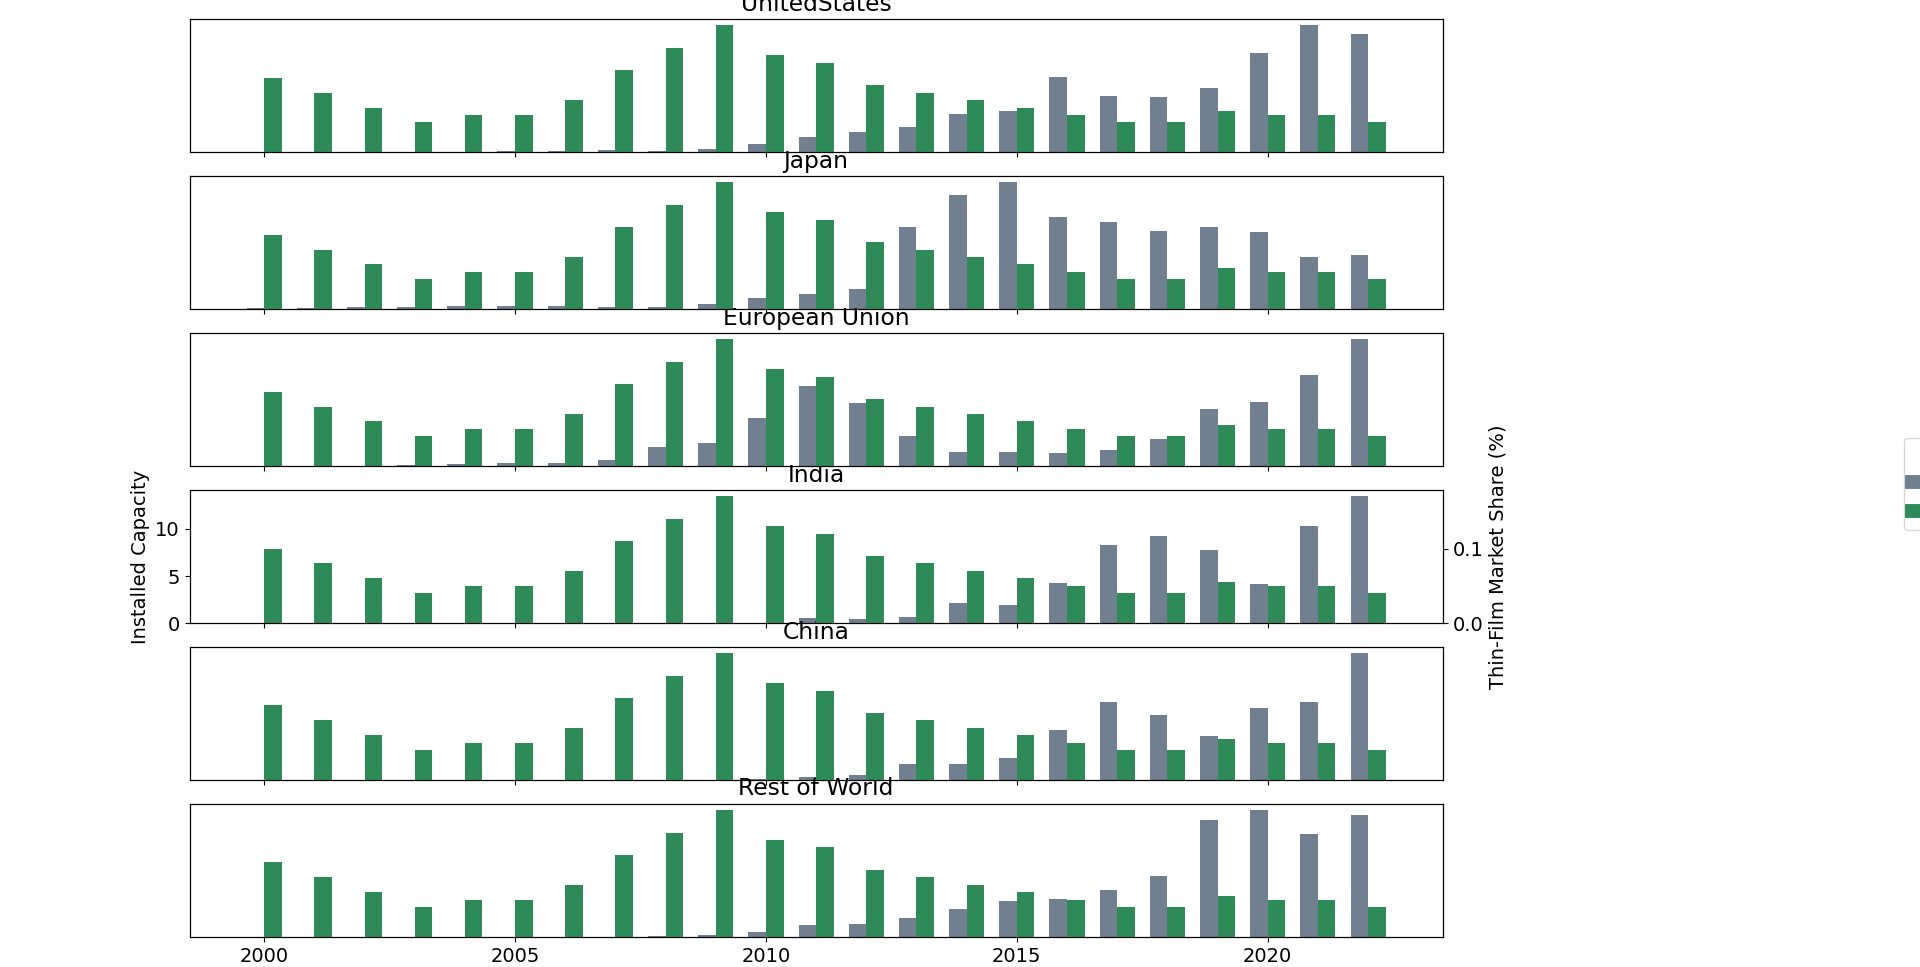
\includegraphics[width=0.5\linewidth]{Figures/Installed Capacity and Thin-film Market Share.png}
%      \caption{Total Capacity Installed and Thin Film Percentage by Country}
%      \label{fig:enter-label}
% \end{figure}

% \begin{figure}
%     \centering
%     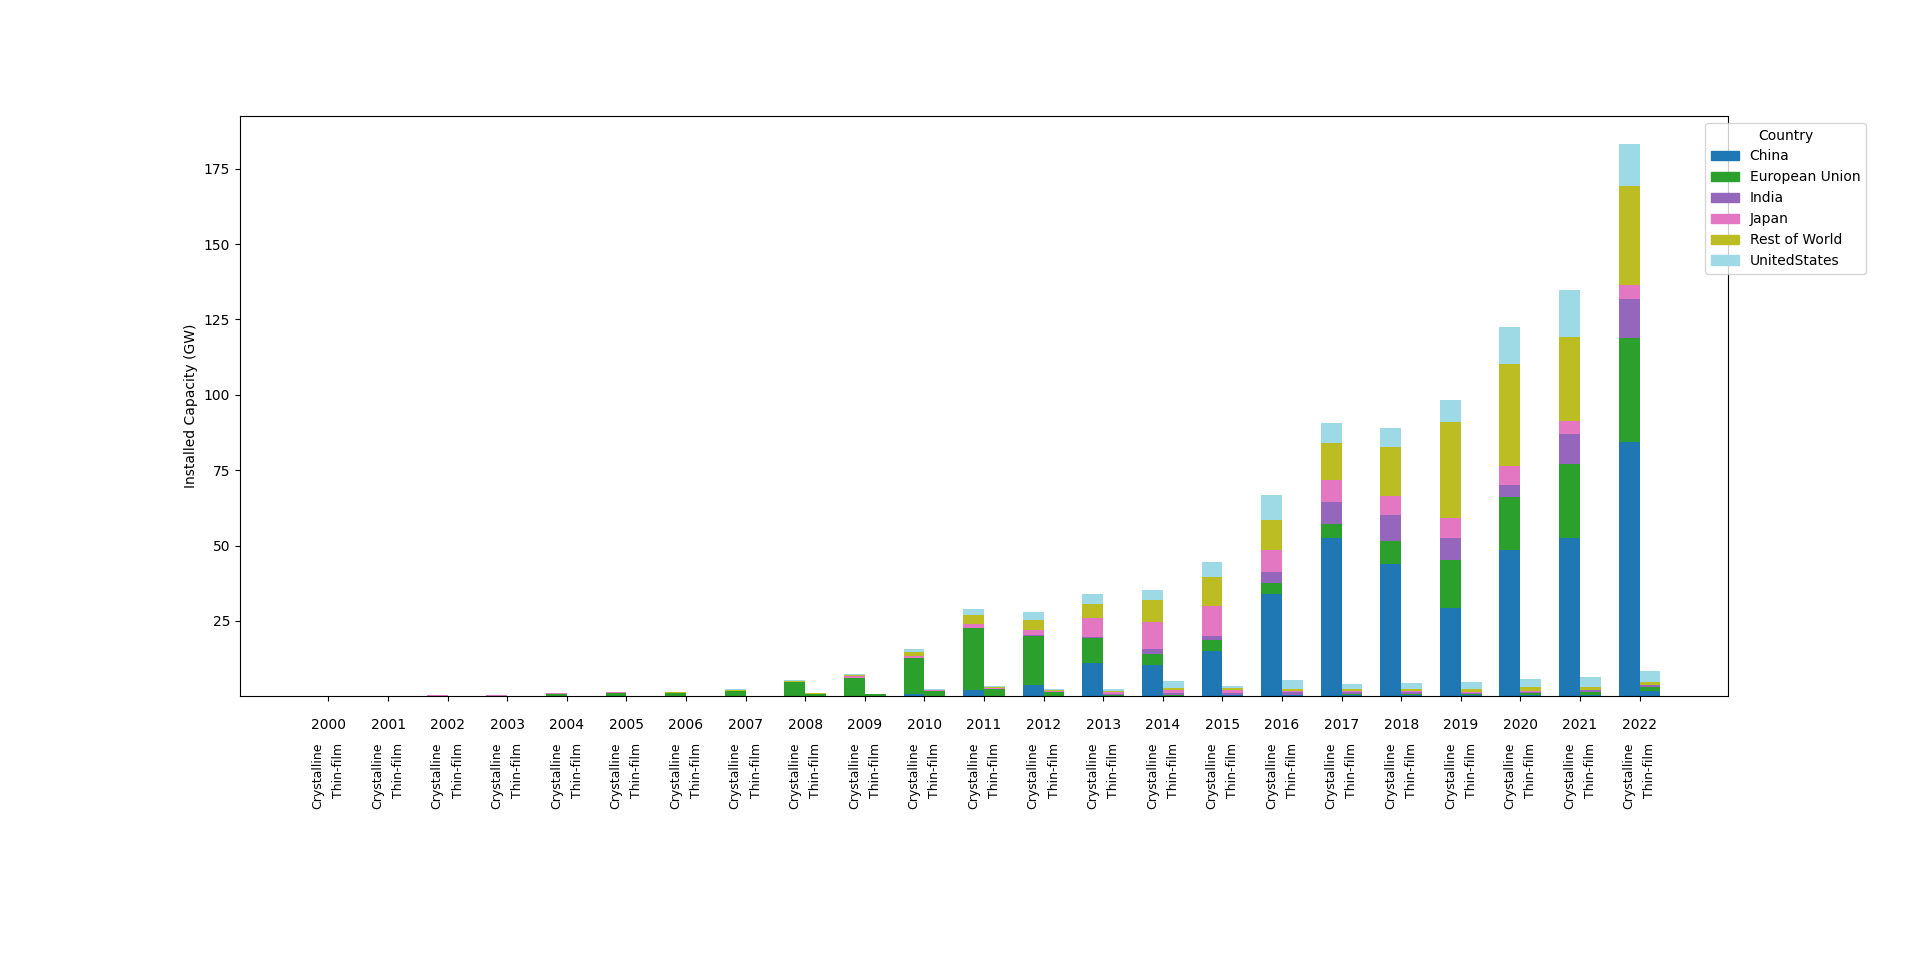
\includegraphics[width=0.5\linewidth]{Figures/Installed Capacity by Country.png}
%     \caption{Total Capacity Installed by Type by Country}
%     \label{fig:enter-label}
% \end{figure}


\begin{figure}[tbh]
\centering
\caption{\label{fig:data_sum_PV_price_region}Solar Panel Price by Region}
\subfloat[c-Si]
{\centering
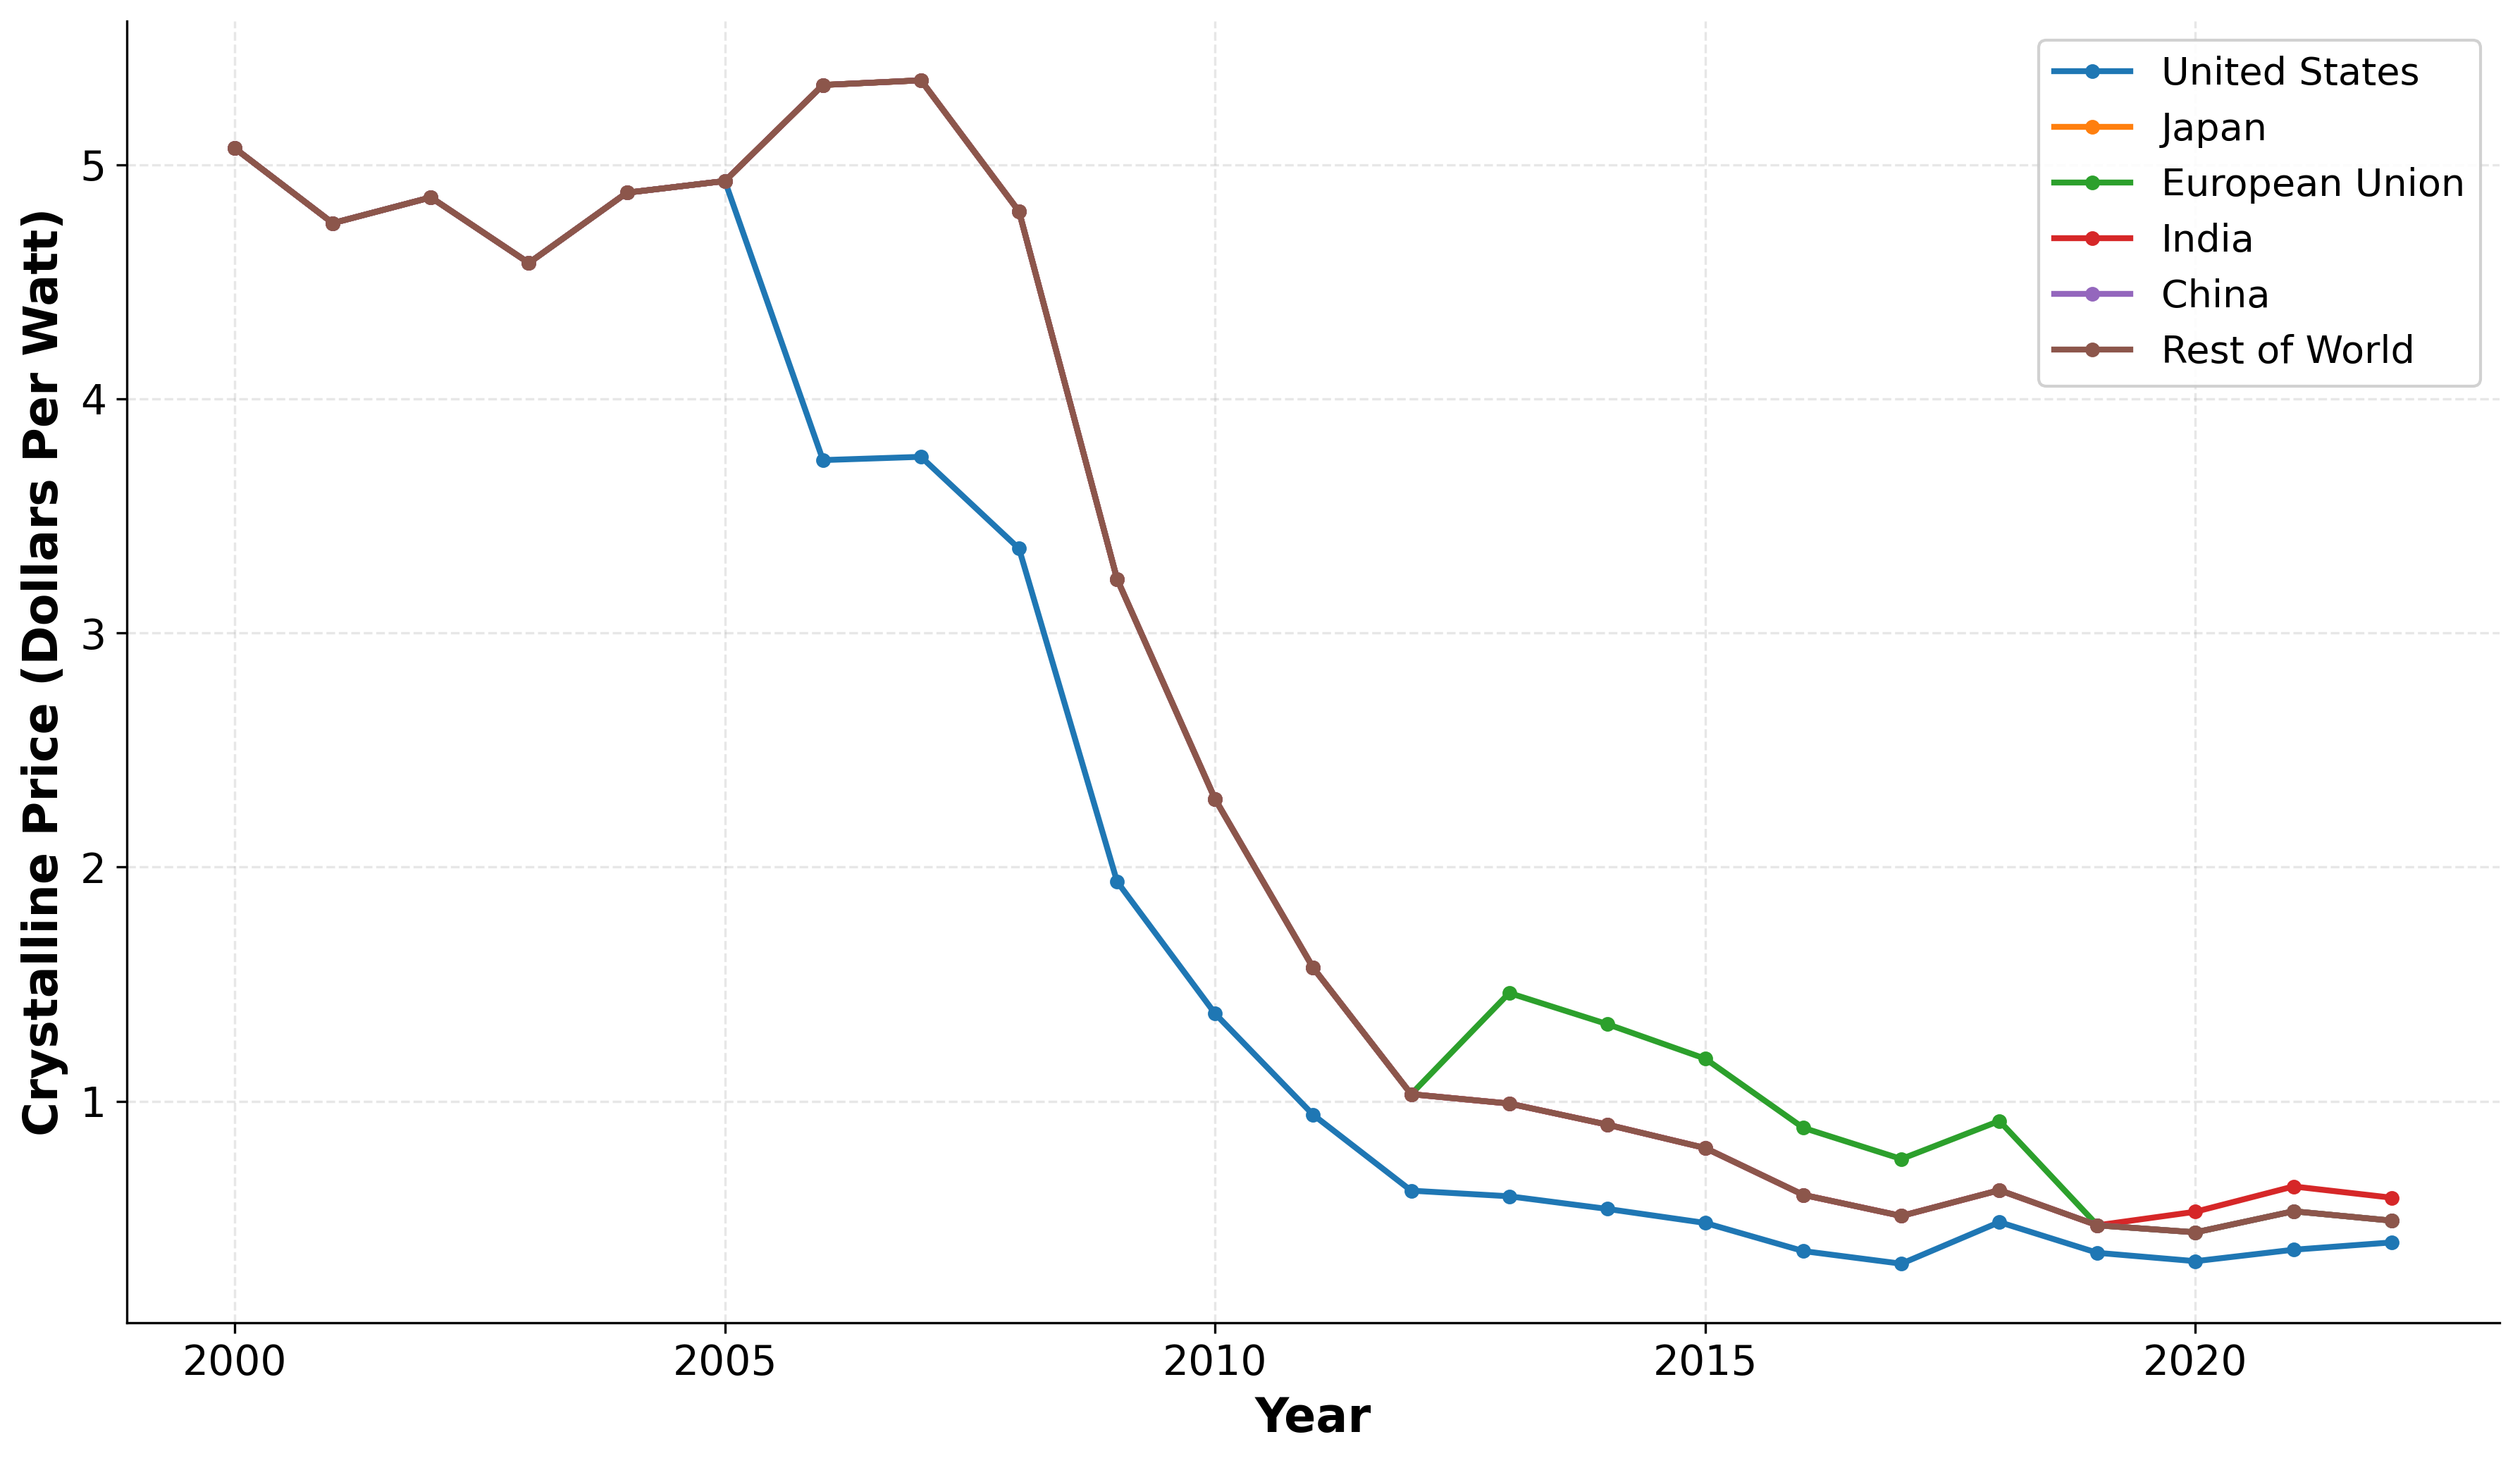
\includegraphics[scale=0.25]{Figures/crystalline_prices_by_country.png}
}
\subfloat[Thin-Film]
{\centering
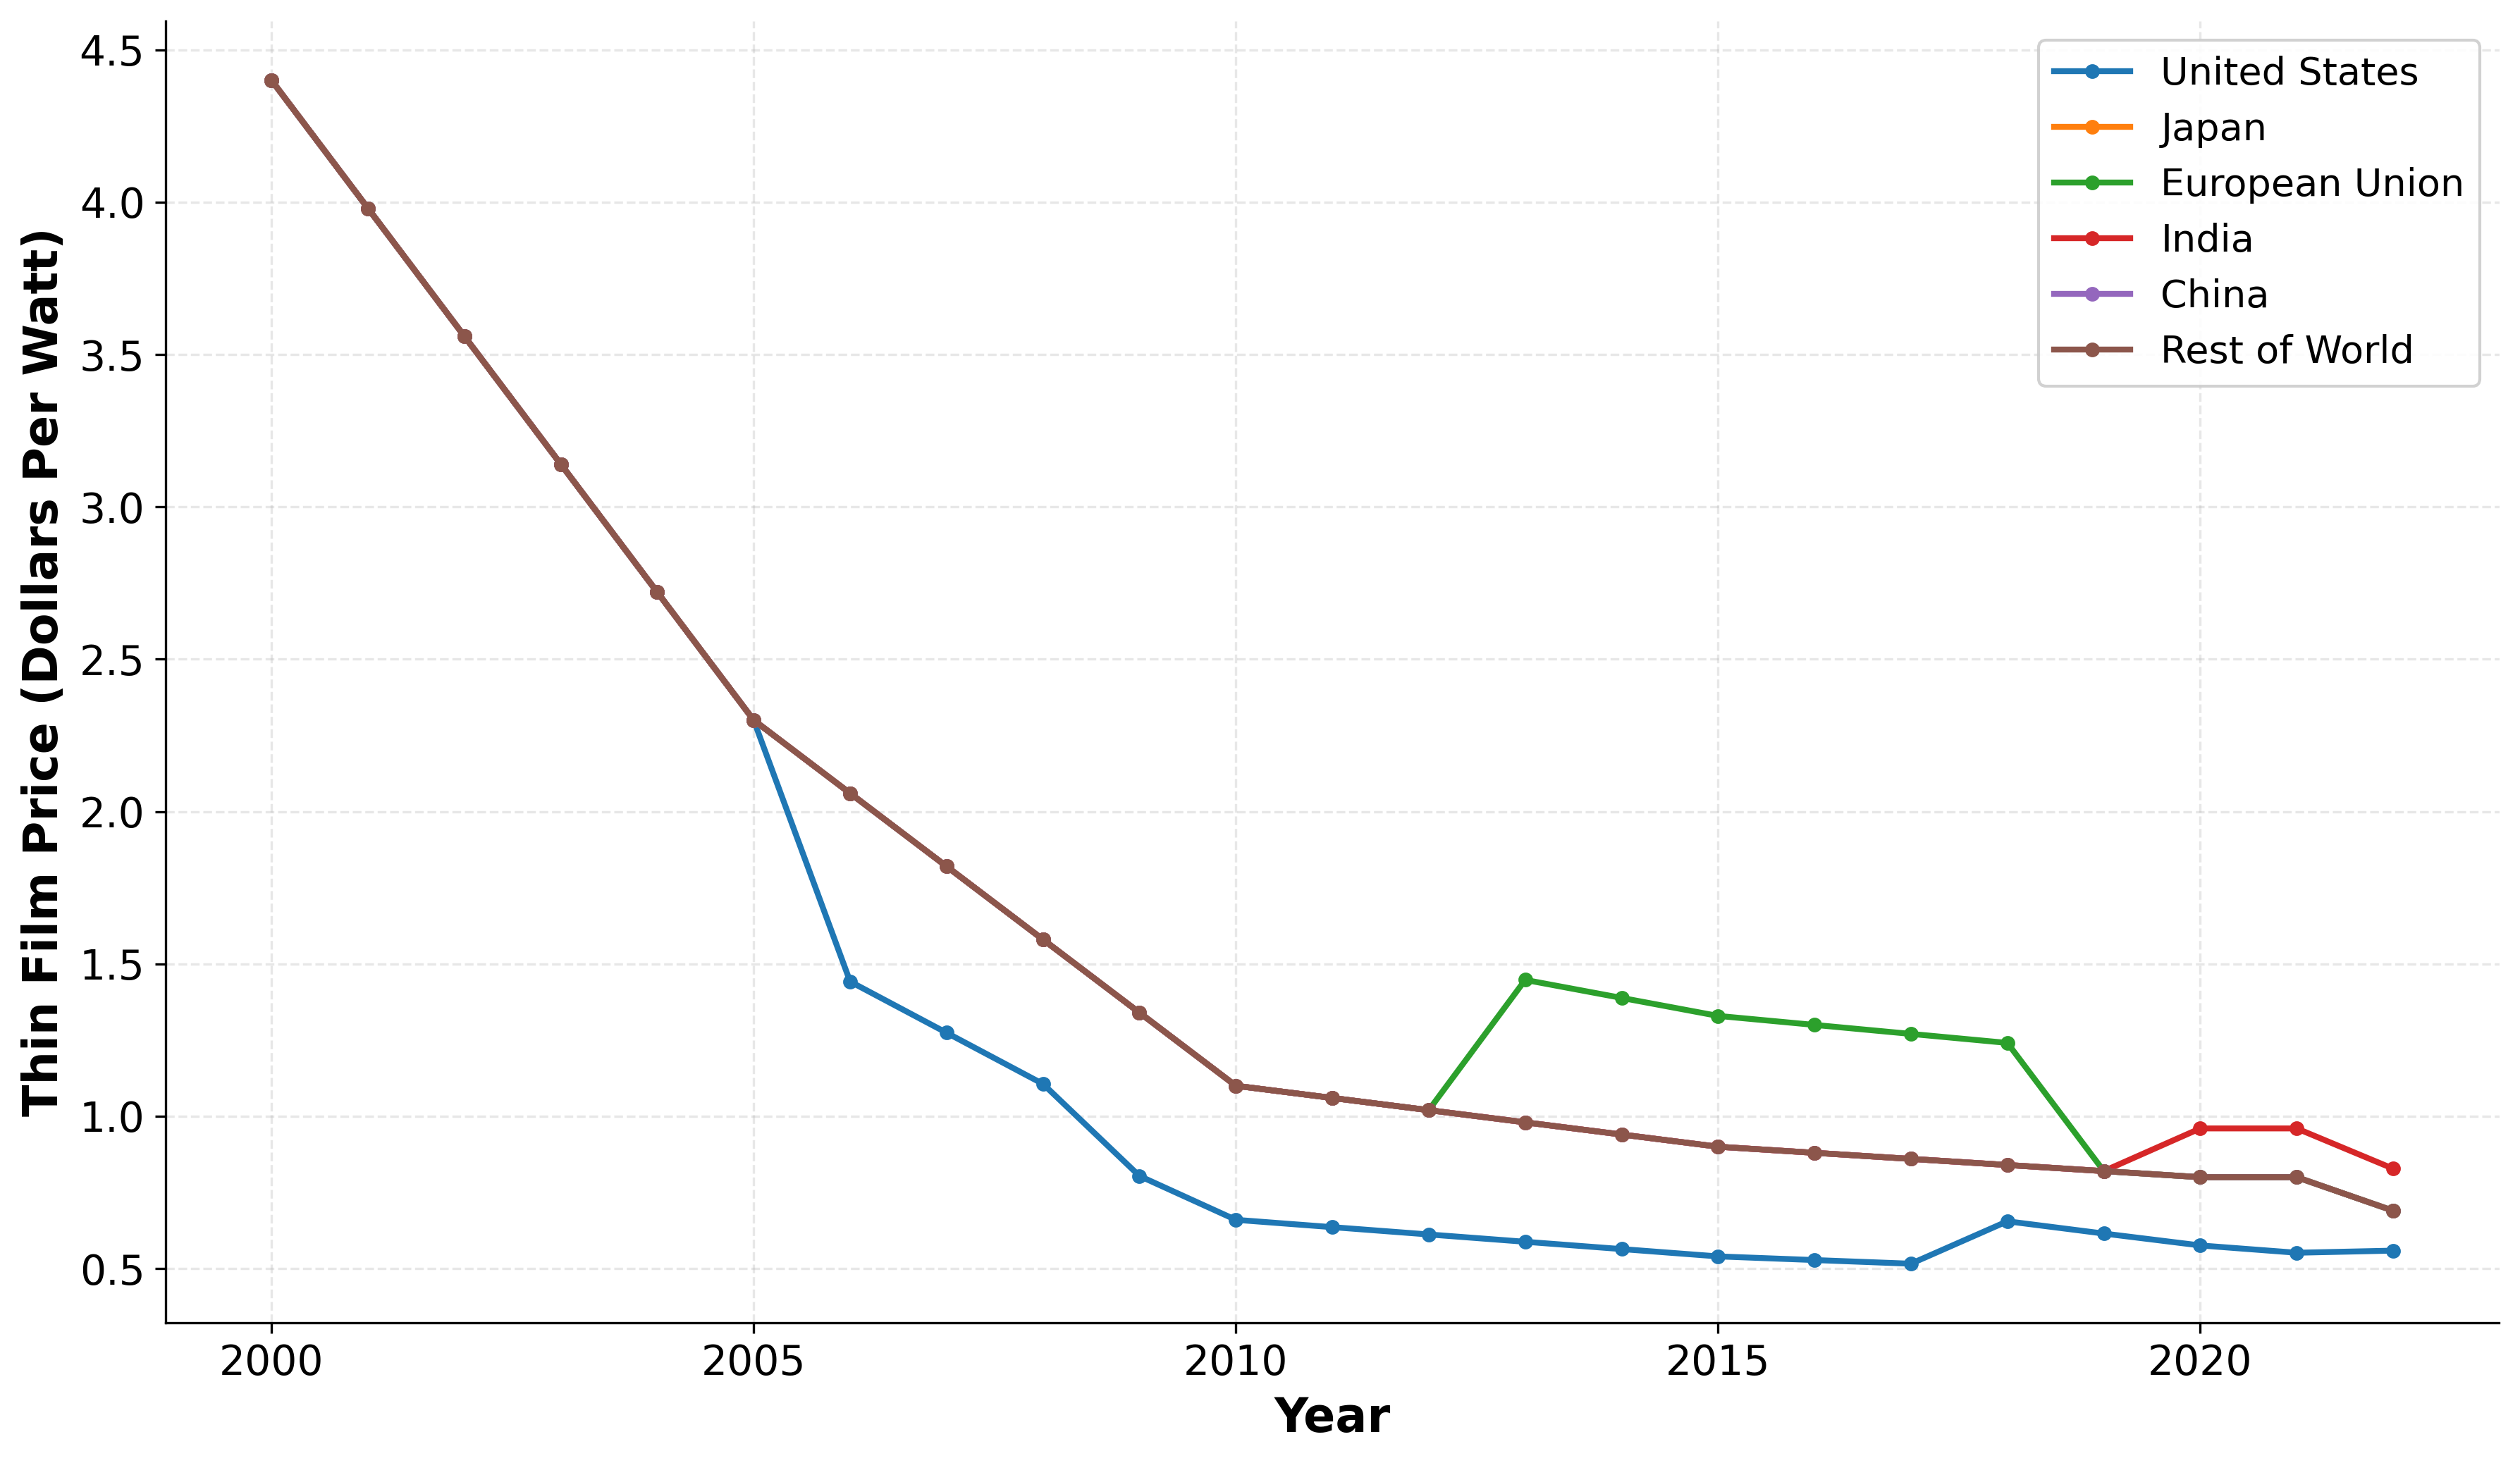
\includegraphics[scale=0.25]{Figures/thinfilm_prices_by_country.png}
}
\end{figure}


\begin{figure}[tbh]
\centering
\caption{\label{fig:data_sum_entry_exit}Entry and Exit of Chinese Solar Panel Manufacturers}
\subfloat[Entry]
{\centering
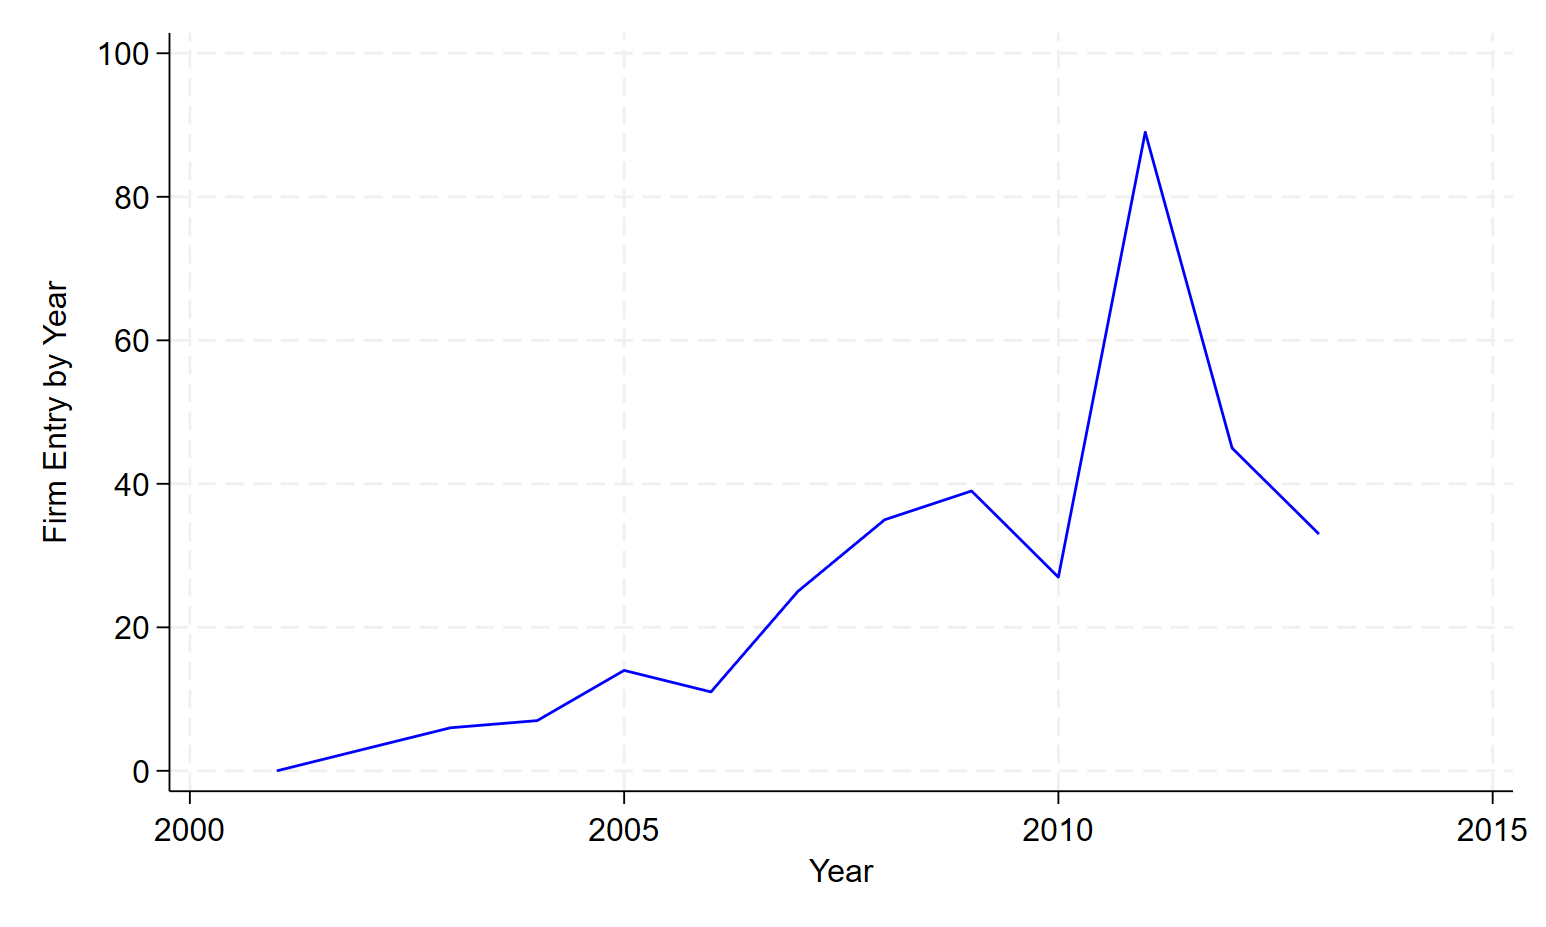
\includegraphics[scale=0.15]{Figures/FirmEntryOverTime.png}
}
\subfloat[Exit]
{\centering
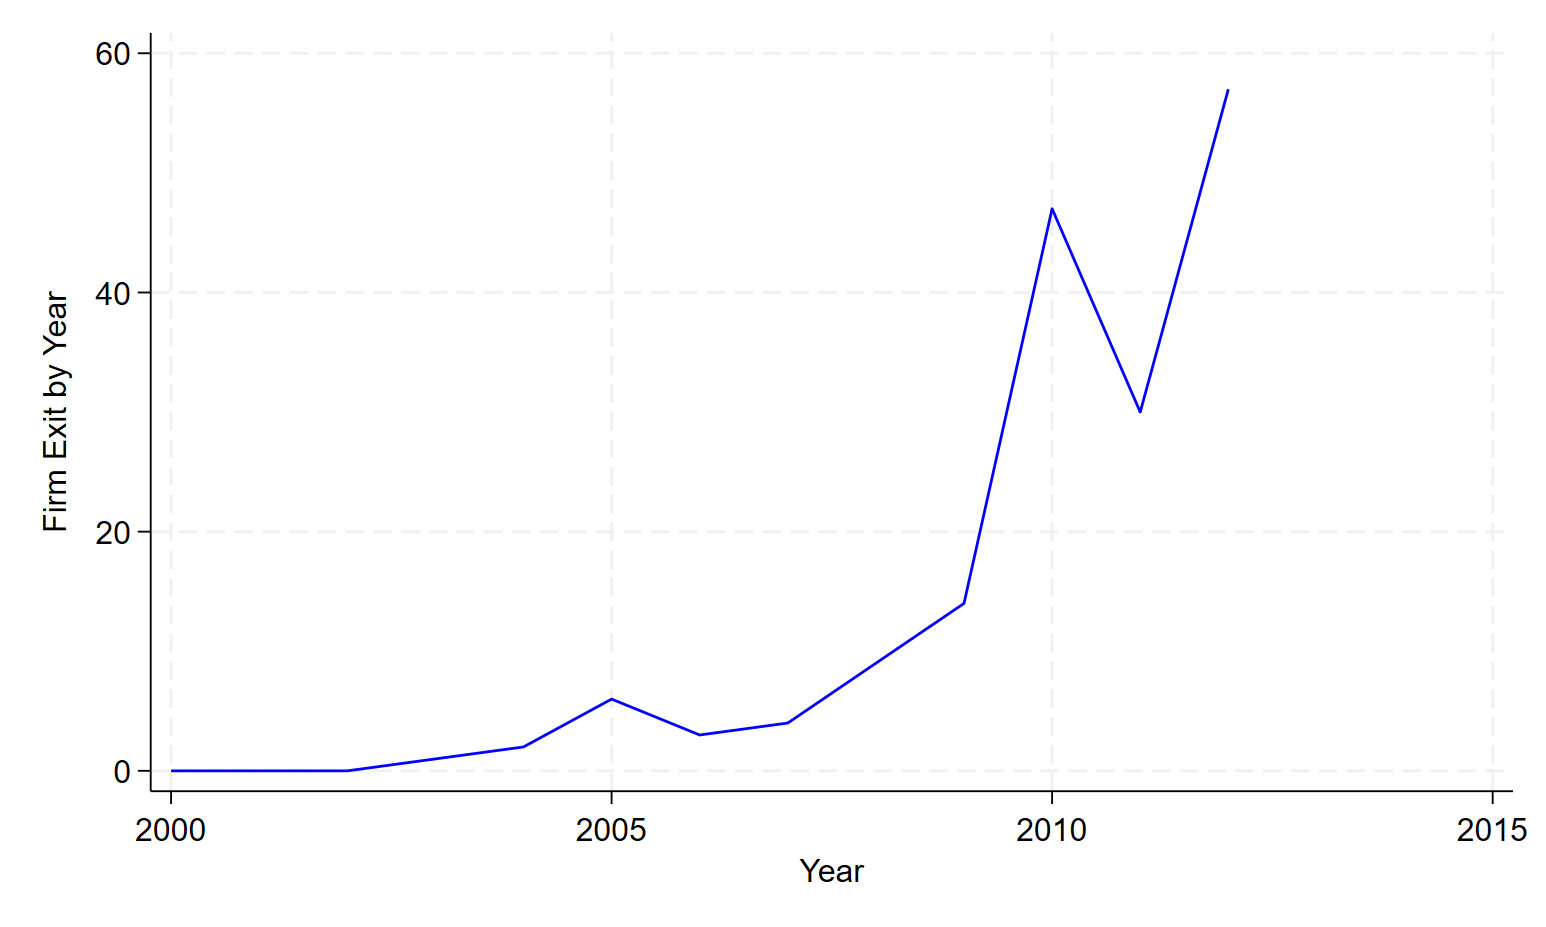
\includegraphics[scale=0.15]{Figures/FirmExitOverTime.png}
}
\end{figure}



\begin{table}[tbh]
\centering
\caption{AR(1) Estimates of State Transition Process}
\label{tab:est_state_transition}
\begin{threeparttable}
\begin{tabularx}{1.00\textwidth}{Xcccccccc}
\toprule
& \multicolumn{2}{c}{Output Price} && \multicolumn{1}{c}{Demand Subsidies} && \multicolumn{3}{c}{Input Price} \\
\cmidrule{2-3} \cmidrule{5-5} \cmidrule{7-9}
 & Poly. & Thin-film && Common && Poly. & Cadmium & Tell. \\
\midrule
$\lambda_0^{pre}$ 
    & 1.596 & -1.570 && 0.021 && 36.799 & 2.272 & 3.238 \\
    & (0.022) & (0.099) && (0.033) && (9.1) & (0.584) & (0.662) \\

$\lambda_0^{post}$ 
    & -1.761 & 7.223 && 0.131 && 6.07 &  &  \\
    & (0.048) & (0.439) && (0.229) && (9.72) &  &  \\

$\lambda_1$  
    & 0.804 &  && -0.053 &&  0.195 & 7.099 & 7.164 \\
    & (0.054) &  && (1.634) && (0.064) & (0.082) & (0.092) \\

\midrule
N 
    & 22 & 22 && 13 && 228 & 31 & 30 \\
$R^2$ 
    & 0.988 & 0.998 && 0.660 && 0.760 & 0.633 & 0.615 \\
AIC 
    & -29.671 & -97.774 &&  &  & 2362.69 & 44.499 & 32.491 \\
\bottomrule
\end{tabularx}
\begin{tablenotes}
    \item Notes: The dependent variable is the price in year $t$. Standard errors in parenthesis. We use different year as the cutoff to define Pre" and Post". The cutoff year is 2008 for the c-Si solar panel and polysilicon price, 2010 for the thin-film solar panel price, 2007 for the Cadmium price, 2011 and for the Tellurium price. The demand subsidies are measured in two ways. \textcolor{blue}{The first one is weighted by a region's share of demand among the all demand, i.e., $\sum_m sub_{mt} * \frac{Q_{mt}}{\sum_{m'}Q_{m't}}$, where $sub_{mt}$ is the demand subsidy in region $m$ and $Q_{mt}$ is the total demand in region $m$. The second one is weighted by the share of a firm's output to a region among this firm's total output, i.e., $\sum_m sub_{mt} * \frac{q_{jmt}}{\sum_{m'}q_{jm't}}$, where $sub_{mt}$ is the demand subsidy in region $m$ and $q_{jmt}$ is firm $j$'s sales to region $m$.} 
    \item Structural break years: Poly solar panel (2009), Thin-film (2010), Input (2019), Cadmium (2007), Tellurium (2001).
\end{tablenotes}
\end{threeparttable}
\end{table}

\end{document}

% --- Restore commands ---
\let\bibliographystyle\origbibliographystyle
\let\bibliography\origbibliography
\let\setcounter\origsetcounter
\let\thispagestyle\origthispagestyle
\let\singlespacing\origsinglespacing
\let\onehalfspacing\origonehalfspacing
\let\small\origsmall

\endgroup

% --- Per-chapter bibliography ---
\singlespacing
\bibliographystyle{chicago}
\bibliography{solar_tech}
\doublespacing


% --- Chapter 3: AI Power Grids ---
% =============================================================================
% Chapter 3: Certificates without Electrons? AI-Driven Power Demand
% Draws content from:
%   ../Energy Economics Submission/Energy_CAS.tex
% Bib file: Energy.bib (in that same folder; found via BIBINPUTS)
% =============================================================================

% --- Set graphics search path for this chapter ---
\graphicspath{{../Energy Economics Submission/}{../Energy Economics Submission/Figures/}}

\chapter{Certificates without Electrons? Theory and Evidence on Impacts from AI-Driven Power Demand}
\label{ch:ai_power}

\begingroup

% --- Suppress front-matter commands ---
\renewcommand{\maketitle}{}%
\renewcommand{\title}[2][]{}%
\renewcommand{\author}[2][]{}%
\renewcommand{\date}[1]{}%

% --- Suppress CAS-specific front-matter commands ---
\renewcommand{\shorttitle}[1]{}%
\renewcommand{\shortauthors}[1]{}%
\renewcommand{\cormark}[1][]{}%
\renewcommand{\ead}[1]{}%
\renewcommand{\credit}[1]{}%
\renewcommand{\cortext}[2][]{}%

% --- Suppress CAS affiliation (takes optional + mandatory arg) ---
\let\origaffiliation\affiliation
\renewcommand{\affiliation}[2][]{}%

% --- Suppress CAS highlights environment ---
\let\orighighlights\highlights
\let\origendhighlights\endhighlights
\renewenvironment{highlights}{\setbox\z@\vbox\bgroup}{\egroup}%

% --- Suppress CAS keywords environment ---
\let\origkeywords\keywords
\let\origendkeywords\endkeywords
\renewenvironment{keywords}{\setbox\z@\vbox\bgroup}{\egroup}%

% --- Suppress bibliography commands (we issue our own below) ---
\let\origbibliographystyle\bibliographystyle
\let\origbibliography\bibliography
\renewcommand{\bibliographystyle}[1]{}%
\renewcommand{\bibliography}[1]{}%

% --- Suppress \appendix so it does not switch chapter numbering globally ---
\renewcommand{\appendix}{}%

% --- Convert wrapfigure to regular figure to prevent text overlapping
%     under double spacing ---
\let\origwrapfigure\wrapfigure
\let\origendwrapfigure\endwrapfigure
\renewenvironment{wrapfigure}[2]{\begin{figure}[htbp]}{\end{figure}}%

% --- Include the essay body (docmute strips preamble) ---
%% 
%% Formatted for Elsevier CAS single-column (cas-sc) template
%% Converted from ACM sigconf format
%% 

\documentclass[a4paper,fleqn,longmktitle]{cas-sc}

\usepackage[authoryear,longnamesfirst]{natbib}

%%% Packages %%%
\usepackage{hyperref}
\usepackage{url}
\usepackage{amsmath,amssymb,amsfonts,amscd,amsthm}
\usepackage{mathrsfs}
\usepackage{algorithmic}
\usepackage{graphicx}
\usepackage{textcomp}
\usepackage{xcolor}
\usepackage{pifont}
\usepackage{verbatim}
\usepackage{threeparttable}
\usepackage{tabularx}
\usepackage{booktabs}
\usepackage{rotating}
\usepackage{wrapfig}
\usepackage{comment}
\usepackage{calc}
\usepackage{multirow}
\usepackage{array}
\usepackage{multicol}
\usepackage{ragged2e}
\usepackage{pgfplots}
\pgfplotsset{compat=1.18}
\usetikzlibrary{pgfplots.groupplots}
\newcommand{\sym}[1]{\ifmmode^{#1}\else\(^{#1}\)\fi}
\usepackage{caption}
\usepackage[english]{babel}
\usepackage{enumerate}
\usepackage{tikz}
\usepackage{bm}
\usepackage{csquotes}
\usepackage[useregional]{datetime2}
\usepackage{bbm}
\usepackage{svg}
\usetikzlibrary{arrows.meta, positioning, decorations.pathreplacing}
\usepackage[export]{adjustbox}
\usetikzlibrary{shapes, arrows.meta, positioning, fit, backgrounds, calc, shadows}
\usetikzlibrary{shapes.geometric}
\usetikzlibrary{intersections}
\usepackage{tcolorbox}
\usepackage{etoolbox}
\usepackage{eurosym}
\usepackage{longtable}
\usepackage{enumitem}

\ExplSyntaxOn
\cs_if_exist:NF \vbox_unpack_clear:N
  { \cs_new_eq:NN \vbox_unpack_clear:N \vbox_unpack_drop:N }
\ExplSyntaxOff

% Define colors for visual mapping
\definecolor{isoBlue}{RGB}{0, 114, 178}
\definecolor{costRed}{RGB}{213, 94, 0}
\definecolor{constrGreen}{RGB}{0, 158, 115}

% Color Scheme
\definecolor{valBlue}{RGB}{0, 114, 178}
\definecolor{profGold}{RGB}{230, 159, 0}
\definecolor{stateGray}{RGB}{100, 100, 100}

% Economics style definitions
\definecolor{econBlue}{RGB}{31, 119, 180}
\definecolor{econRed}{RGB}{214, 39, 40}
\definecolor{econGold}{RGB}{188, 143, 46}

% Consistent Color Palette
\definecolor{fossilRed}{RGB}{196, 69, 54}
\definecolor{fossilRedLight}{RGB}{248, 229, 227}
\definecolor{reGreen}{RGB}{46, 125, 50}
\definecolor{reGreenLight}{RGB}{232, 245, 233}
\definecolor{primaryBlue}{RGB}{26, 54, 93}
\definecolor{primaryBlueLight}{RGB}{232, 238, 245}
\definecolor{accentOrange}{RGB}{217, 119, 6}
\definecolor{mutedGray}{RGB}{73, 80, 87}
\definecolor{surfaceGray}{RGB}{248, 249, 250}

% TikZ styles
\tikzset{
    econAxis/.style={thick, ->, >=stealth},
    supply/.style={thick, econRed},
    demand/.style={thick, econBlue},
    priceLine/.style={thin, gray, densely dashed},
}

%%% MACROS %%%
\newcommand{\nb}[1]{\textcolor{blue}{NB[#1]}}
\newcommand{\aruna}[1]{\textcolor{blue}{Aruna[#1]}}

\begin{document}
\let\WriteBookmarks\relax
\def\floatpagepagefraction{1}
\def\textpagefraction{.001}

% Short title
\shorttitle{Empirical Impacts from AI-Driven Power Demand}

% Short author
\shortauthors{Golden, Balasubramanian, Balasubramanian}

% Main title
\title[mode = title]{Certificates without Electrons? Theory and Evidence on Impacts from AI-Driven Power Demand}

% First author
\author[1]{Dana Golden}
\cormark[1]
\ead{dana.golden@stonybrook.edu}
\credit{Conceptualization, Methodology, Software, Data Curation, Formal Analysis, Writing -- Original Draft, Writing -- Review \& Editing, Visualization}

\affiliation[1]{organization={Department of Economics, Stony Brook University},
            city={Stony Brook},
            postcode={11794},
            state={New York},
            country={USA}}

% Second author
\author[2]{Aruna Balasubramanian}
\ead{arunab@cs.stonybrook.edu}
\credit{Conceptualization, Writing -- Review \& Editing, Supervision}

\affiliation[2]{organization={Department of Computer Science, Stony Brook University},
            city={Stony Brook},
            postcode={11794},
            state={New York},
            country={USA}}

% Third author
\author[2]{Niranjan Balasubramanian}
\ead{niranjan@cs.stonybrook.edu}
\credit{Conceptualization, Writing -- Review \& Editing, Supervision}

% Corresponding author text
\cortext[1]{Corresponding author}

\begin{abstract}
Data centers now account for 4.4\% of United States electricity demand, yet the grid-level effectiveness of the renewable energy certificates (RECs) and power purchase agreements (PPAs) hyperscalers use to claim carbon neutrality remains unclear. We develop a game-theoretic model in which a data center operator chooses among RECs, PPAs, and behind-the-meter colocation while generators make entry decisions under endogenous financing costs. The model identifies a timing wedge—the mismatch between consumption and credited renewable generation—as a central mechanism through which AI demand degrades reliability, raises prices, and increases emissions even when RECs cover 100\% of annual consumption. Colocation with storage addresses this wedge directly and induces the greatest renewable entry by eliminating generator revenue risk.
We test these predictions by exploiting the staggered release of large language models as a natural experiment, using difference-in-differences on a novel dataset linking AI activity to local grid outcomes. AI demand significantly increases fossil generation, wholesale prices (up to 25\% in treated PJM zones), and outage frequency (0.5–1 additional outages per year) near data centers, with impacts scaling in model size. Data centers with on-site generation exhibit a sign reversal in power-quality effects, consistent with the model's prediction that behind-the-meter capacity absorbs demand spikes. Counterfactual analyses show that edge inference, spatial reallocation, and colocated storage each substantially mitigate grid impacts, while REC-only strategies do not. Together, our results demonstrate that the externalities of AI to the grid are tightly coupled to procurement design and the spatial organization of data center infrastructure.
\end{abstract}

% Research highlights
\begin{highlights}
\item First causal estimates of AI model releases on U.S.\ power grid stability using staggered difference-in-differences
\item AI activity degrades power quality equivalent to 0.5--1 additional outages per year and increases fossil fuel demand by hundreds of GWh
\item Wholesale electricity prices increase up to 25\% in treated PJM zones during AI model activity periods
\item On-site colocated generation and distributed edge inference substantially mitigate grid impacts
\end{highlights}

% Keywords
\begin{keywords}
Artificial intelligence \sep Power grids \sep Electricity markets \sep Reliability \sep Power quality \sep Econometrics \sep Difference-in-differences
\end{keywords}

\maketitle

\section{Introduction}\label{sec:intro_aipower}

\begin{wrapfigure}{H}{0.45\linewidth}
    \centering
    \vspace{-10pt}
    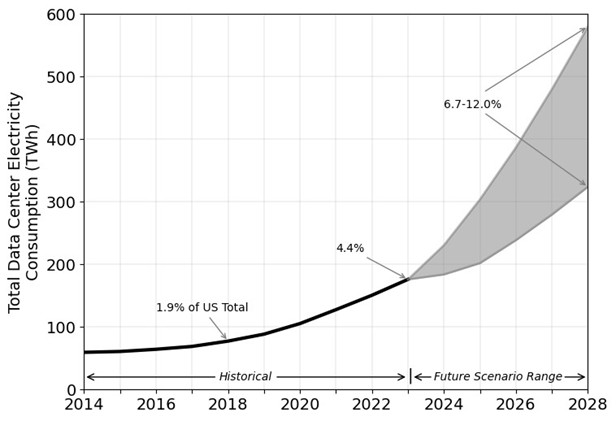
\includegraphics[width=.8\linewidth]{Figures/Data Center Electricity Consumption over Time (1).jpg}
    \caption{Projected data center growth over time. Source: DOE.}
    \label{fig:DataCenterGrowth}
    \vspace{-10pt}
\end{wrapfigure}
 
Over the past six years, data centers have expanded from consuming 1.9\% to 4.4\% of total U.S.\ electricity demand (Figure~\ref{fig:DataCenterGrowth}, DOE). This rapid growth---driven largely by artificial intelligence---follows two decades of essentially flat electricity consumption and coincides with nationwide efforts to electrify transport and heating. Grid infrastructure was planned for stable demand, not simultaneous load growth from multiple sectors. The combination raises fundamental questions about how AI-driven electricity demand affects reliability, prices, and emissions---and whether the procurement instruments that hyperscalers use to meet voluntary clean energy commitments are adequate to address these externalities.
 
Data center hyperscalers have responded to scrutiny over their growing electricity footprint by purchasing renewable energy certificates (RECs) and signing power purchase agreements (PPAs), often claiming carbon-neutral or ``100\% renewable'' operations on this basis. Yet the economics of these instruments suggest reasons for skepticism. RECs are financial transfers that do not alter real-time dispatch; a hyperscaler that retires RECs on an annual basis may still draw power from fossil generators during every hour of peak demand. PPAs contract for renewable output but do not guarantee temporal alignment between generation and consumption. Whether these instruments meaningfully reduce the grid-level externalities of AI workloads---or primarily serve as accounting devices---is an open empirical question with significant policy implications.
 
Our paper makes two contributions to address it. First, we develop a game-theoretic model of hyperscaler electricity procurement in which a large data center operator chooses between RECs, PPAs, and behind-the-meter colocation, while generators make entry decisions under endogenous financing costs. The model yields sharp predictions. Because renewable generation is intermittent, incremental data center demand raises fossil generation---and therefore emissions and prices---unless storage or colocation can shift clean energy into the hours when load is highest. We formalize this as the \emph{timing wedge}: the gap between when a hyperscaler consumes electricity and when its contracted or credited renewable generation actually produces. REC purchases do not shrink this wedge in the short run; PPAs reduce it only modestly absent firming; colocation with storage addresses it directly by physically supplying the data center with renewable energy in real time. The model further predicts an investment hierarchy driven by financing risk: colocation eliminates revenue variance for generators and therefore induces the greatest renewable entry, followed by PPAs, then merchant REC arrangements. The paradoxical implication is that even a hyperscaler purchasing RECs to cover 100\% of its annual load can simultaneously degrade local reliability, raise wholesale prices, and increase system-wide emissions. Colocation with storage and generation substantially mitigates these outcomes.
 
Second, we provide the first causal estimates of these grid-level externalities. Exploiting the staggered release of frontier large language models (LLMs) as a natural experiment, we use difference-in-differences methods to estimate how AI model training and inference affect local power quality, fossil fuel generation, and wholesale electricity prices. The empirical results are consistent with the model's predictions. We find that large model releases cause significant power quality deterioration---well above half the standard deviation of U.S.\ power quality distributions---and increase fossil fuel consumption on the order of hundreds of GWh during both training and inference phases. Wholesale electricity prices increase substantially in treated zones, with increases of up to 25\% in the American Electric Power (AEP) zone of PJM. Critically, we find that data centers with on-site generation exhibit a sign reversal in power quality effects relative to those without, consistent with the model's prediction that behind-the-meter generation absorbs demand spikes that would otherwise propagate to the grid. Impact magnitudes scale with model size, suggesting that these externalities will grow as frontier models continue to expand.
 
Our theoretical and empirical analyses jointly speak to an active policy debate. Proposals for hourly renewable matching---such as those advanced under the 24/7 Carbon-Free Energy framework---attempt to close the timing wedge by requiring temporal alignment of clean energy credits with consumption. Our model provides a framework for evaluating such proposals: tightening the granularity parameter $h$ raises effective REC prices in high-carbon hours and increases the private value of storage and temporally aligned generation, shrinking the timing wedge in equilibrium through both entry and operational responses. We complement the model's comparative statics with descriptive analysis of REC and PPA markets, documenting the gap between contracted clean energy and real-time grid conditions that gives rise to the timing wedge in practice.
 
The paper also contributes methodologically. Because proprietary operational data on AI workloads are unavailable, we construct a novel dataset linking publicly available power grid data, data center locations, AI model release dates, and market prices. We use publicly announced model training and release dates as plausibly exogenous shocks and apply staggered difference-in-differences estimation \citep{cengiz2019effect, deshpande2019screened} to address variation in treatment timing across models and locations. We validate our identification strategy through parallel trends tests, placebo exercises with randomized treatment dates and locations, alternative geographic boundary definitions, and time series anomaly detection. To address supply-side confounds in the fossil fuel demand analysis, we instrument for electricity prices using the interaction of generator-level heat rates and regional natural gas prices.
 
This work connects four literatures. It contributes to the economics of electricity markets by documenting a new and rapidly growing source of demand-side pressure on wholesale prices and grid reliability \citep{borenstein2002trouble, joskow2008capacity}. It advances the literature on environmental externalities from industrial electricity consumption \citep{fowlie2012industrial, greenstone2014environmental} by showing that voluntary procurement instruments may fail to internalize the externalities they are designed to address. It engages the emerging literature on the energy and environmental footprint of AI \citep{strubell19, schwartz2020green, morrison2025holistically} by moving from facility-level accounting to system-level causal estimation. Finally, it informs the policy debate over renewable energy procurement design \citep{miller2022hourly} by providing both a theoretical framework and empirical evidence for evaluating alternative matching granularities.
 
The remainder of the chapter proceeds as follows. Section~\ref{sec:relatedwork} reviews related work. Section~\ref{sec:model} presents the game-theoretic model, including the toy model that illustrates core mechanisms and the full model with equilibrium characterization. Section~\ref{sec:empirical} describes the empirical setting, data construction, and econometric methodology. Section~\ref{Sec::Results} presents estimation results. Section~\ref{sec:counterfactuals} reports counterfactual analyses examining alternative AI development trajectories. Section~\ref{sec:conclusion_aipower} concludes.

\section{Related Work}\label{sec:relatedwork}

This paper contributes to four interrelated economics literatures: wholesale electricity market design, environmental externalities from industrial electricity consumption, renewable energy procurement and corporate carbon accounting, and the emerging empirical literature on data center grid impacts.
 
\subsection{Wholesale Electricity Markets and Demand Shocks}
 
The institutional foundations of U.S. wholesale electricity markets are well established. \citet{borenstein_bushnell2015} provide a comprehensive assessment of restructuring outcomes, documenting that wholesale price formation via locational marginal pricing remains sensitive to demand conditions due to the convex shape of the aggregate supply curve and limited short-run demand elasticity \citep{borenstein2002trouble}. In this setting, large demand increases---such as those from data center load---move clearing prices up the supply curve and may amplify market power rents \citep{borenstein2002measuring, borenstein_bushnell1999}. \citet{bushnell_mansur_saravia2008} show that vertical arrangements and forward contracting dramatically affect wholesale prices in restructured markets, a finding relevant to the bilateral power purchase agreements increasingly used by hyperscalers.
 
Transmission constraints further shape how demand shocks propagate. \citet{borenstein_bushnell_stoft2000} analyze how limited transmission capacity creates localized price effects---precisely the mechanism through which geographically concentrated data center load elevates LMPs in constrained corridors. \citet{joskow2008capacity} identifies the ``missing money'' problem in capacity markets, directly relevant as PJM capacity prices rose from \$30 to \$270/MW-day between 2023 and 2024, partly driven by data center growth \citep{cmu2025}. \citet{joskow2019} further documents how intermittent renewable generation complicates wholesale market investment signals, a challenge amplified when new baseload demand from data centers coincides with coal retirements and renewable expansion.
 
The merit-order literature provides the inverse mechanism to our analysis. While \citet{sensfuss2008} and \citet{cludius2014} show that zero-marginal-cost renewables shift supply rightward and depress wholesale prices, data center demand shifts demand rightward, moving clearing prices up the supply curve. This symmetry motivates our focus on wholesale price effects as a primary outcome.
 
\subsection{Environmental Externalities and Marginal Emissions}
 
A large literature documents how industrial electricity consumption generates environmental externalities that vary dramatically by location and time. \citet{siler_evans2012} provide the first systematic calculation of marginal emissions factors for the U.S. grid, revealing substantial regional variation. \citet{graff_zivin2014} extend this framework to show more than threefold variation in marginal emissions across regions, with direct implications for evaluating how data center siting decisions affect net emissions. \citet{holland2022pnas} demonstrate that despite declining \emph{average} grid emissions, \emph{marginal} CO$_2$ emissions from U.S. electricity generation have not decreased---a critical finding for assessing the true environmental impact of incremental data center demand. \citet{callaway_fowlie2018} quantify how the location of demand reduction or renewable generation affects emissions displacement, directly relevant to data center siting.
 
The emissions leakage literature provides further context. \citet{fowlie2009} shows that incomplete cap-and-trade regulation achieves only a fraction of intended emissions reductions due to leakage across jurisdictional boundaries. \citet{fell_maniloff2018} provide empirical evidence that RGGI caused coal generation to shift to non-participating states. These mechanisms are directly applicable to data centers: load growth in one region can increase fossil fuel dispatch in neighboring regions, undermining the environmental benefits of local renewable procurement. \citet{holland2016aer} demonstrate that externalities from electricity-intensive activities in one state are substantially exported to others via the interconnected grid.
 
\subsection{Renewable Energy Certificates and Corporate Procurement}
 
A growing literature evaluates the environmental effectiveness of corporate clean energy procurement strategies. \citet{gillenwater2008a} establishes that unbundled RECs fail credible additionality tests, and \citet{gillenwater2014} shows empirically that the voluntary REC market has negligible influence on the economic feasibility of new wind projects. \citet{bjorn2022} find that when REC-based emission reductions are removed from corporate inventories, companies' scope~2 trajectories no longer align with climate targets. \citet{brander2018} identify fundamental problems with the GHG Protocol's market-based method that allows hyperscalers to claim zero scope~2 emissions via REC purchases.
 
System-level modeling confirms this hierarchy. \citet{xu2024} provide the first comprehensive comparison of annual volumetric matching, hourly (24/7) matching, and emissions-based matching strategies, finding that annual matching via RECs does little to reduce system-level emissions while hourly matching is significantly more effective. \citet{riepin2024} find similar results in European markets, estimating that 98\% hourly carbon-free energy matching carries a 54\% cost premium over annual matching but substantially reduces system emissions. On the PPA side, \citet{backstrom2023} use U.S.\ county-level data with two-way fixed effects to show that corporate PPAs have influenced aggregate renewable capacity---unlike voluntary RECs---though effects are heterogeneous across contract types and regions.
 
These findings motivate our game-theoretic procurement model. The empirical literature establishes a clear hierarchy of environmental effectiveness---unbundled RECs (lowest), annual volumetric matching, and 24/7 hourly matching (highest)---that maps onto the strategic choices available to hyperscalers in our framework.
 
\subsection{Data Center Grid Impacts}
 
Our paper contributes most directly to the emerging empirical literature on data center electricity market impacts. \citet{benetton2023} establish the template for studying how large, geographically concentrated computing loads create electricity price externalities: using Bitcoin price as an exogenous demand shifter in Upstate New York, they find that cryptocurrency mining raised electricity costs by \$92 million annually for small businesses and \$204 million for households. We extend this approach to AI-driven data center demand, using model releases rather than cryptocurrency prices as the demand shock.
 
Several concurrent papers study data center grid impacts using complementary methods. \citet{mamkhezri2025} use difference-in-differences examining Virginia data center expansion on wholesale prices across census tracts, finding that interconnections raise wholesale prices by 7.3\% through congestion and marginal loss components. \citet{kay2026} develop an hourly least-cost dispatch model covering all U.S.\ wholesale markets, finding existing data centers have increased wholesale prices by 3--5\% nationally, with substantially larger effects in data center corridors and projected increases of 20--50\% under high-utilization scenarios. \citet{bogmans2025} use a multi-country CGE model to project U.S.\ electricity price increases of 8.6\% and carbon emissions increases of 5.5\% from AI-driven data center growth. \citet{knittel2025} model data center flexibility in PJM, ERCOT, and WECC, finding that flexible scheduling reduces system costs but has ambiguous emissions effects depending on the generation mix.
 
On the political economy side, \citet{gargano2025} study state-level tax incentives for data centers using staggered DiD, finding that incentives increase development but with limited employment impacts. \citet{jacobs2025} documents \$4.3 billion in transmission connection costs passed to PJM ratepayers.
 
Our paper differs from this literature in three respects. First, our game-theoretic procurement model connects the empirical findings on price and emissions externalities to the strategic incentives facing hyperscalers, bridging the gap between the market impact and corporate procurement literatures. Second, we use AI model releases as plausibly exogenous demand shocks, providing an identification strategy that does not rely on observing facility-level capacity additions. Third, we examine power quality degradation alongside price effects, capturing externalities beyond the wholesale market.
 

\section{Industry Background}
% % \nb{One possibility is to roll this in with the problem definition in 3.1 if we need space.}
% % \nb{We should also have related work in terms of what kinds of analysis has been done and explain what our work contributes hasnt been done or not easily inferrable from existing work.}
U.S. data centers are expanding rapidly, nearly tripling from its 2008 levels to 1489 active sites in 2025, with another 1,359 on the horizon~\cite{aterio_us_data_centers_2025}. The market is dominated by \emph{hyperscalers}---vertically integrated data centers---owned by AI heavy companies such as Amazon, Microsoft, and Google, alongside a long tail of smaller operators. Hyperscalers afford companies certain economies of scale but greatly increase the geographic concentration of power demand on the grids. Concentrated demand strains local grids in the area, raising congestion costs and sometimes degrading power quality for neighboring consumers. Large, inflexible loads from AI hyperscalers also reduce system reliability, elevate wholesale prices, and complicate renewable integration.
\subsection{Market Overview}

The U.S. data center market has expanded rapidly, growing from 519 facilities in 2008 to 1,489 active sites in 2025, with another 1,359 announced or under construction \cite{aterio_us_data_centers_2025}. Electricity demand more than tripled over this period, rising from under 5 to over 15 GWh per hour (BNEF), while total U.S. capacity increased only 17.6\% \cite{EIA_2023_table4_2A} and dispatchable baseload capacity fell as coal retired.
Power consumption has risen in parallel, though since 2018 growth in renewable generation has outpaced data center demand as shown in Figure \ref{fig:DCPowerConsumption}.

\begin{wrapfigure}{l}{0.45\linewidth}
    \centering
    \vspace{-10pt}
    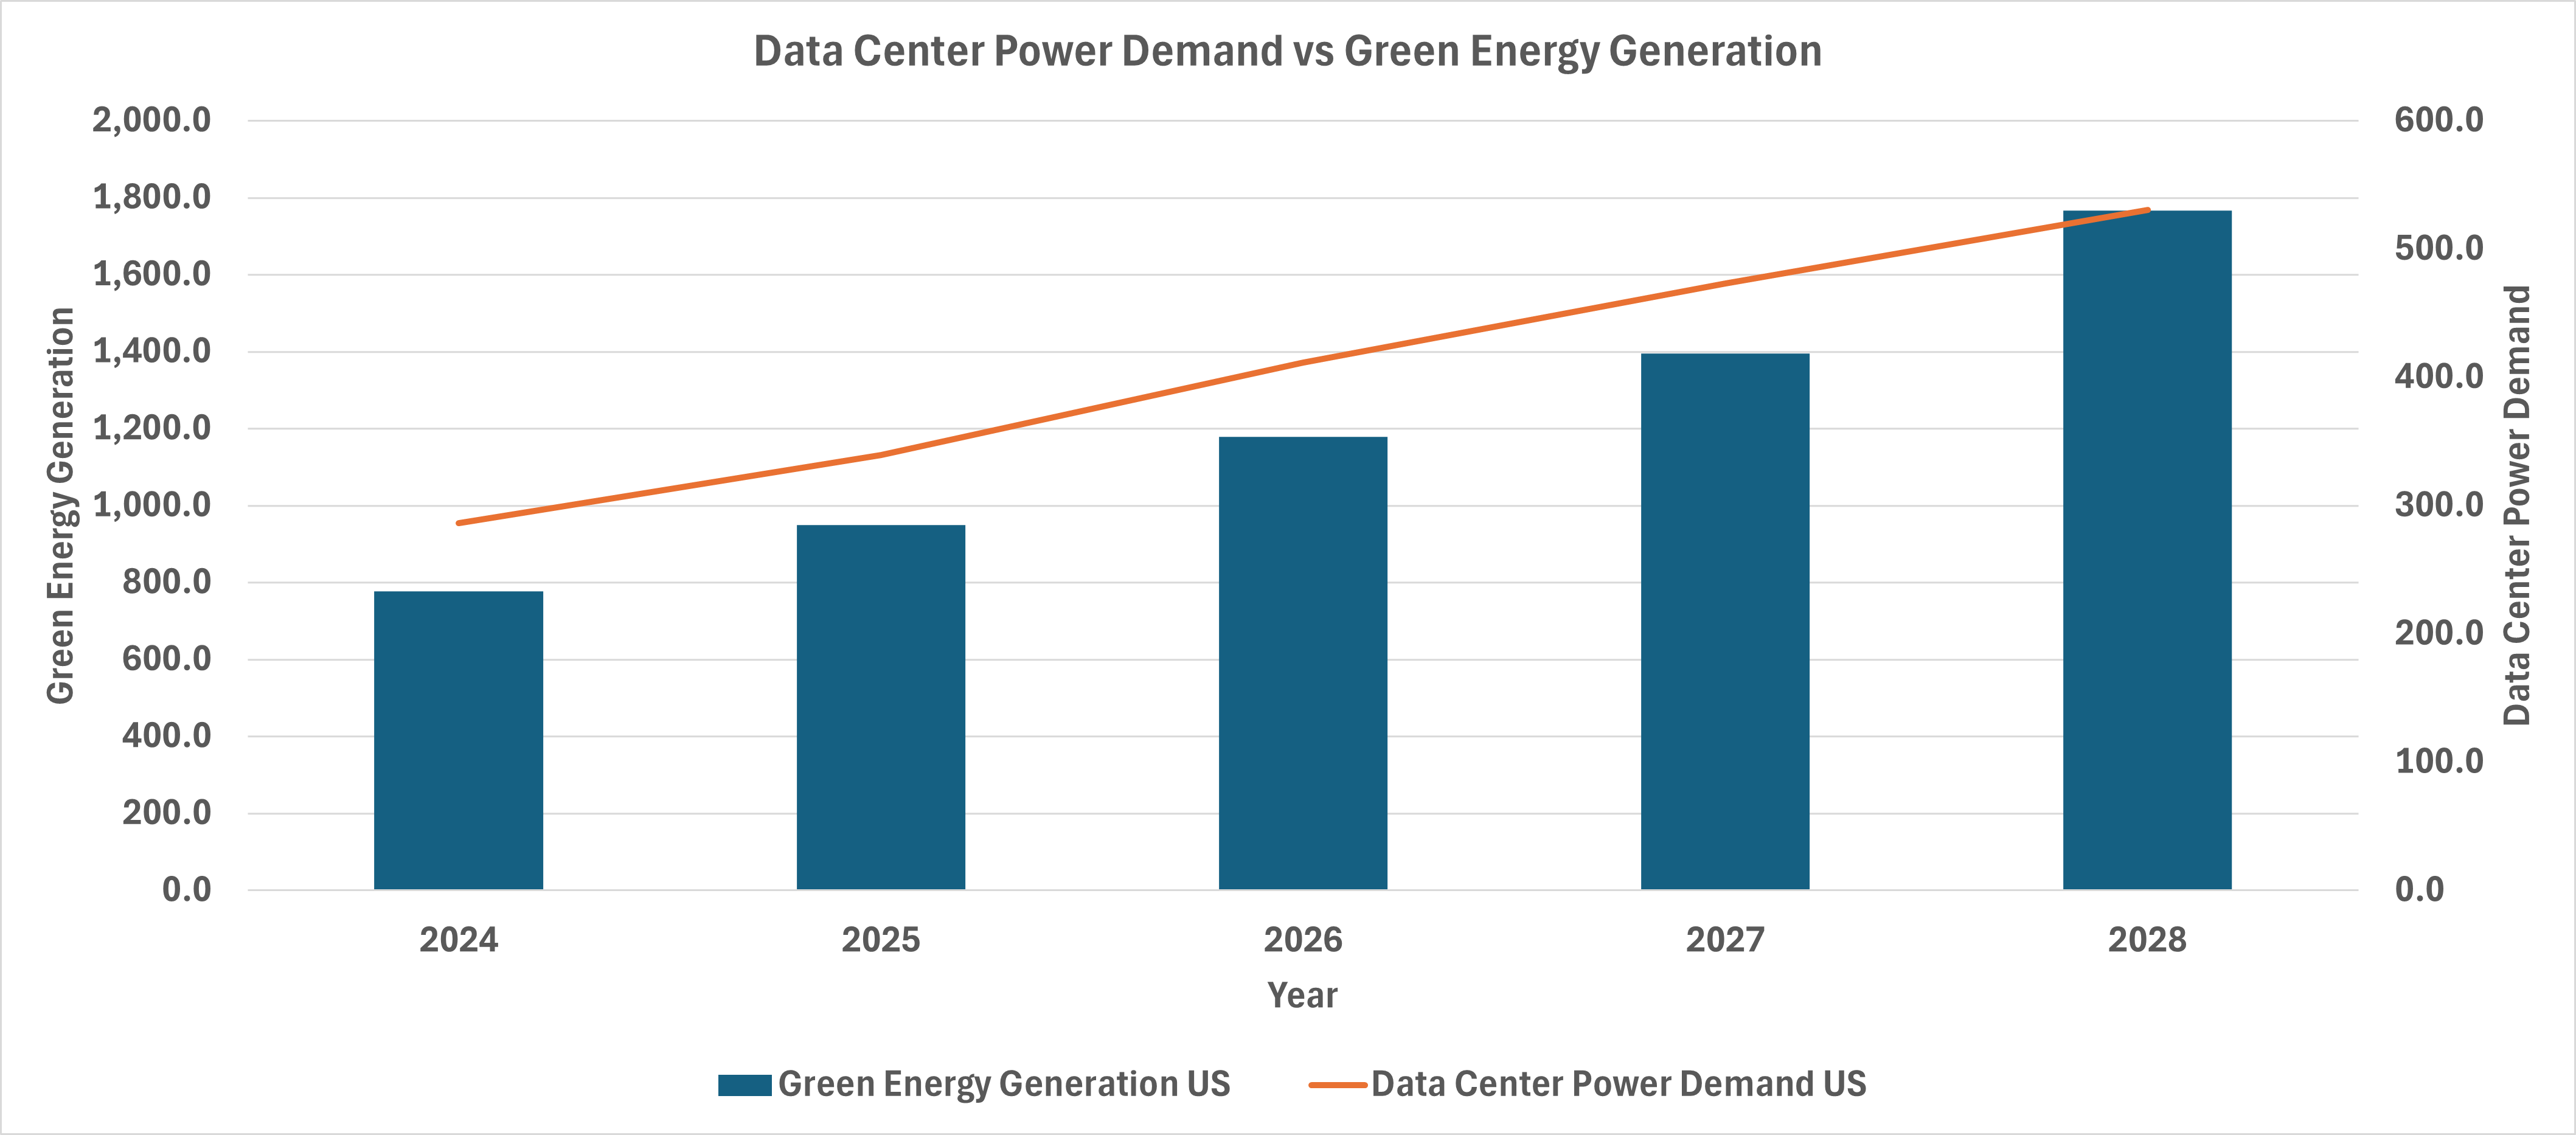
\includegraphics[width=\linewidth]{Figures/Data Center Power Demand vs Green Generation.png}
    \caption{Data center power consumption vs.\ green generation. Source: Aterio.io.}
    \label{fig:DCPowerConsumption}
    \vspace{-10pt}
\end{wrapfigure}

The market is geographically concentrated and dominated by hyperscalers—Amazon, Microsoft, and Google—who account for 38\% of capacity across five firms, and 64\% across twenty. Unlike colocation providers such as Equinix, hyperscalers are vertically integrated, owning facilities, long-term power contracts, fiber networks, and custom chips.


\begin{figure}[t!]
    \centering
    % First figure
    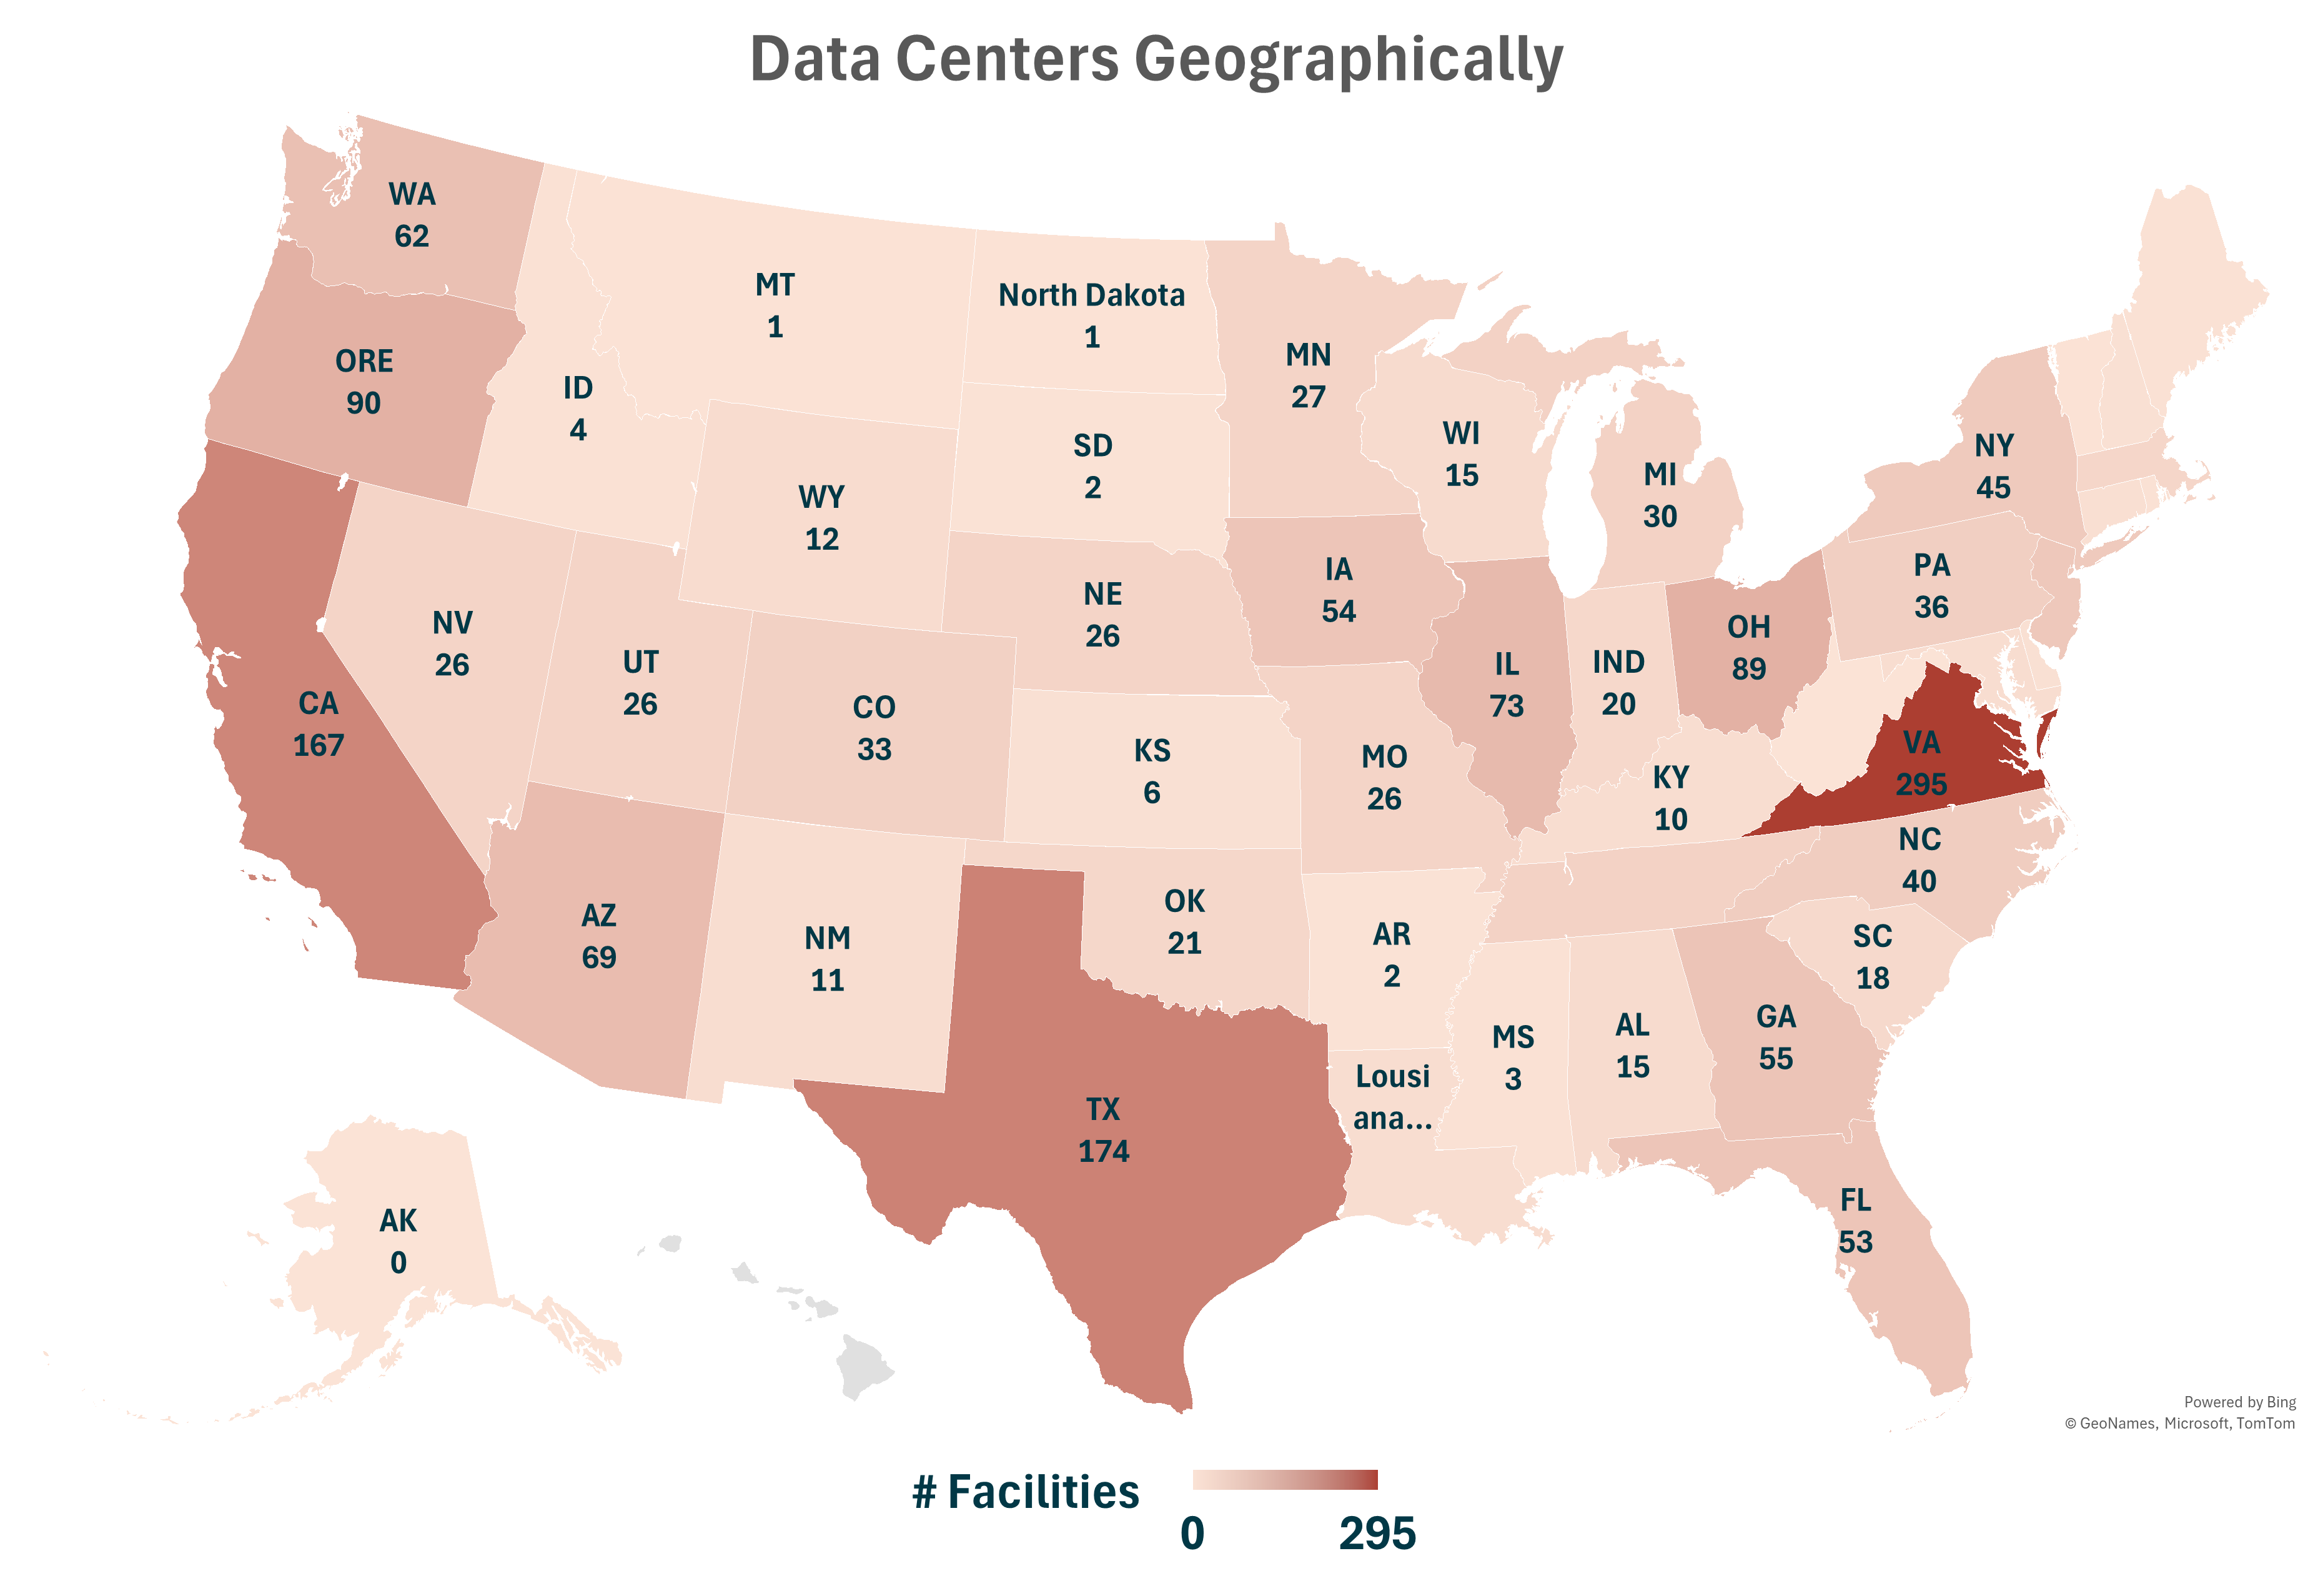
\includegraphics[width=\linewidth]{Figures/Data Centers by State.png}
        \caption{Data centers by state. Source: Aterio.io.}
        \label{fig:DCbyState}
\end{figure}

These economies of scale, however, generate externalities. Concentrated demand in specific regions strains local grids, raising congestion costs and sometimes degrading power quality for neighboring consumers. Large, inflexible loads reduce system reliability, elevate wholesale prices, and complicate renewable integration. At the same time, clustering provides local benefits through jobs, tax revenues, and downstream services. Data centers thus act as both efficiency drivers and sources of regional externalities. It is important to consider the mitigation of the externalities to the grid when analyzing the impacts of AI. We focus on hyperscalers in our paper because hyperscalers perform the majority of AI training and also because larger facilities are more likely to cause power distortions.
% \aruna{Is there a reason why we are talking about hyperscalers? Should we say therefore we focus on these hyperscalers?}

The industry is also geographically concentrated. Texas, California, and especially Virginia dominate U.S. capacity. Virginia’s cluster reflects historic federal investments in internet infrastructure and the routing of early traffic through Northern Virginia. More recent growth in Texas stems from lower electricity costs and streamlined permitting.

The electricity market includes three separate components: generation, transmission, and distribution. Generation is how power is produced. Transmission involves long-range transportation of electricity while distribution involves local distribution of electricity. In the United States, there are two primary models of how the electricity market is structured: vertically integrated utilities and deregulated markets. In vertically integrated utilities, which are prevalent in the South and West, generation, distribution, and transmission are all owned and operated by one company whereas in deregulated markets generation bids in wholesale markets to provide power to utilities, which own transmission and distribution, and provide power in the retail markets. Figure \ref{fig:ISOMap} provides a map showing the geographic makeup of the American electricity market.

\begin{figure}
    \centering
    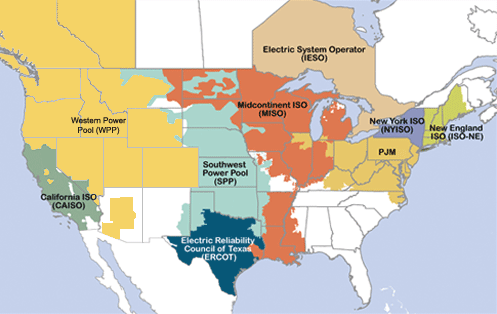
\includegraphics[width=0.5\linewidth]{Figures/ISOMap.png}
    \caption{Map of American electricity market.}
    \label{fig:ISOMap}
\end{figure}

These dynamics interact with broader shifts in the electricity market: greater electrification and the transition from fossil fuels to renewables. Because renewables are intermittent and less dispatchable, rising data center loads coupled with greater renewable penetration place dual pressures on grids, shaping both market outcomes and policy debates. It is therefore crucial to quantify how much power AI uses, how it distorts quality and impacts prices, and the role of efficiency improvements and developments in computing.

% \subsection{Total Harmonic Distortion}
\begin{wrapfigure}{r}{0.3\linewidth}
    \centering
    \vspace{-18pt}
    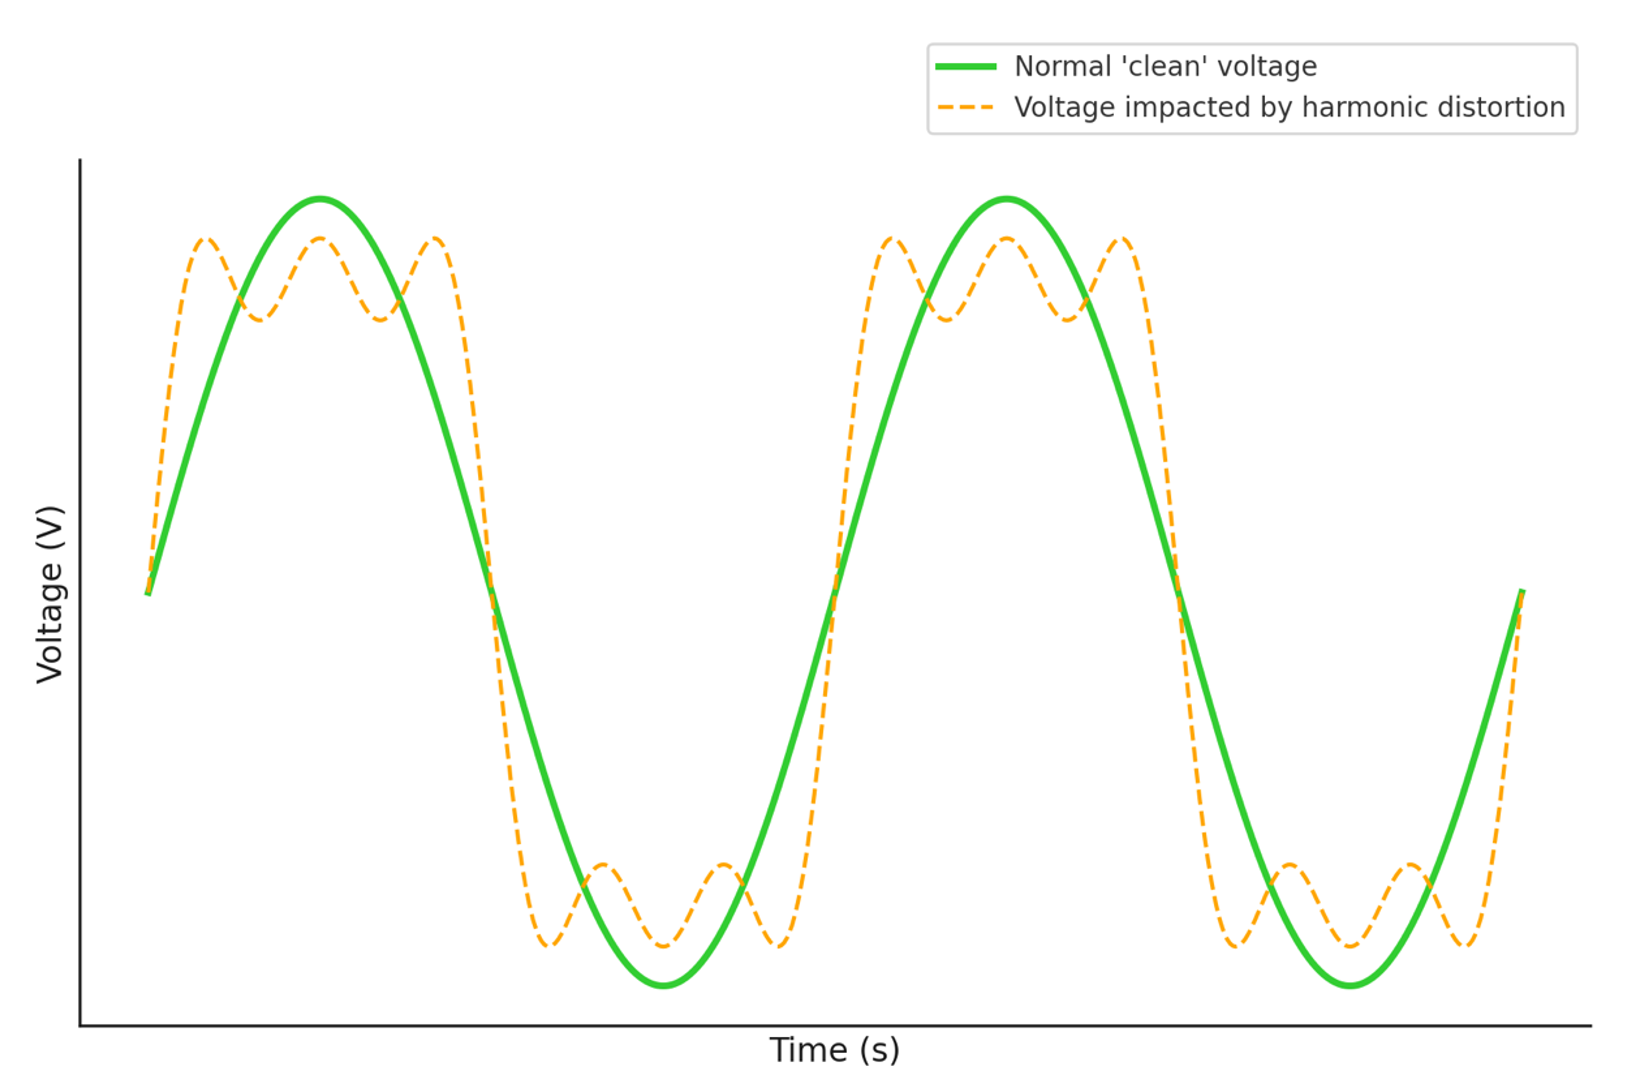
\includegraphics[width=\linewidth]{Figures/HarmonicDistortion.png}
    \caption{Total harmonic distortion representation.}%\aruna{this figure is not referenced in the text}}        
    \label{fig:THD}
    \vspace{5pt}
\end{wrapfigure}
% Figure~\ref{fig:THD} illustrates the distortions in the power frequencies. The green line shows the \emph{clear} voltage curve, which is cleanly sinusoidal, whereas with huge loads can produce harmonic distortions shown as the dotted yellow curve. This \emph{dirtier} voltage can adversely affect the operation and lifetime of household appliances and other products that use electricity.

\subsection{Background: Data Center Concentration and Power-Quality}

AI workloads affect power quality through three main mechanisms. First, data centers and AI computing facilities add substantial baseload demand that can strain grid capacity and compromise voltage regulation, especially during peak periods. Second, AI workloads fluctuate rapidly with computational needs, creating unpredictable load variations that challenge stability and frequency regulation. Third, the switching power supplies and electronics essential to AI hardware generate harmonic distortion, introducing waveform distortions that spread through distribution networks and degrade power quality. Figure~\ref{fig:THD} illustrates the distortions in the power frequencies. The green line shows the \emph{clear} voltage curve, which is cleanly sinusoidal, whereas with huge loads can produce harmonic distortions shown as the dotted yellow curve. This \emph{dirtier} voltage can adversely affect the operation and lifetime of household appliances and other products that use electricity.

\begin{wrapfigure}{r}{0.3\linewidth}
    \centering
    \vspace{-18pt}
    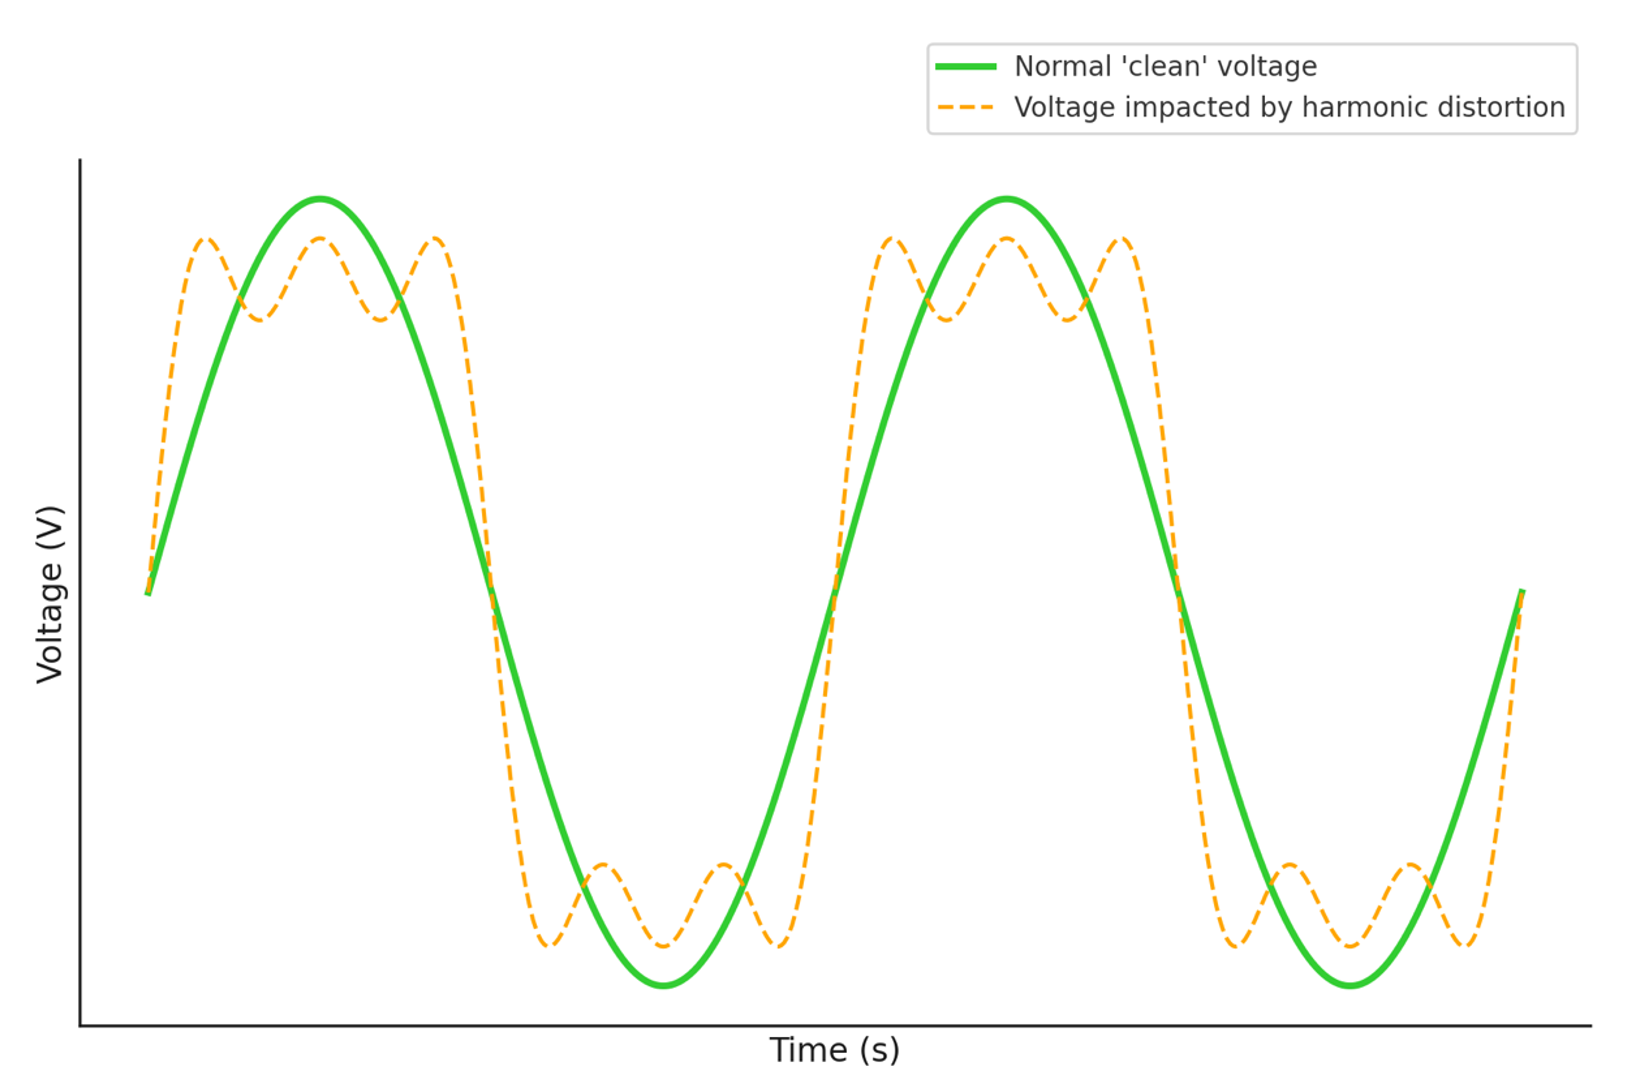
\includegraphics[width=\linewidth]{Figures/HarmonicDistortion.png}
    \caption{Total harmonic distortion representation.}%\aruna{this figure is not referenced in the text}}        
    \label{fig:THD}
    \vspace{5pt}
\end{wrapfigure}

AI workloads also affect wholesale electricity prices through the demand channel, with potentially indeterminate long-run retail market impacts. The U.S. electricity sector comprises both vertically integrated utilities and restructured markets featuring competitive wholesale generation alongside monopoly retail distribution. Wholesale prices are determined hourly in day-ahead markets via sealed-bid, uniform-price auctions subject to network constraints. Locational price variation reflects transmission limitations within the network. Increased demand raises wholesale prices by necessitating dispatch of higher-cost marginal generators.

Wholesale prices are passed through to retail consumers with substantial lag. Retail rates typically reflect average procurement and distribution costs plus a state-regulated return on investment, calculated from historical data. This passthrough mechanism is indirect even absent investment-related dynamics. While new demand sources could theoretically dilute system-wide fixed costs and reduce average retail prices, increased demand more likely raises retail rates. Understanding wholesale demand and price shifts thus provides useful intuition regarding the direction and magnitude of retail price changes.

\subsection{RECs, PPAs, and Colocation}
Corporate electricity procurement takes several forms. Each procurement option entails distinct implications for grid externalities. The most common method is direct procurement, in which a facility draws power as a standard load-serving customer, inheriting the emissions profile of the local generation mix. Often but with increasing rarity and due to the structure of the market, data centers participate directly in the retail electricity market and only interact with utilities.

Despite purchases of electricity with the same properties of that delivered to all other buyers, many hyperscalers claim that they use only renewable electricity. How can this be? To claim renewable attributes without altering physical electron flows, many data center operators purchase renewable energy certificates (RECs). RECs unbundle the environmental attributes of renewable generation into tradeable commodities representing one MWh of renewable output. RECs originated as compliance instruments for state renewable portfolio standards \citep{epa_rec_definition,wiser2004alternative}. REC markets are regulated at the local level with differing standards across markets. Some markets require retirement of RECs in the same geographic market to count. A data center in PJM cannot retire RECs from an ERCOT wind farm. However, this is mostly statutory and is less impactful for voluntary REC purchases. Other markets include voluntary purchases that impose no spatial or temporal constraints.  This disconnect underlies the ``timing wedge'' identified in this paper—annual 100\% renewable claims coexisting with fossil-heavy consumption during peak hours. Empirical evidence suggests the emissions-reduction value of unbundled RECs may be near zero in many markets \citep{bjorn2022recs,gillenwater2007recs}.

Power purchase agreements (PPAs) offer a closer link between procurement and consumption. As shown in Figure \ref{fig:PPAFigure}, PPAs by data centers have risen precipitously since 2016 and have grown alongside data center power consumption. While most PPAs were historically wind-based, battery and solar PPAs are increasingly common, and nuclear PPAs are emerging as a favorite of industry leaders. Physical PPAs deliver contracted renewable power to the offtaker's node, while virtual (financial) PPAs provide contract-for-differences settlements without physical delivery, sharing the spatial mismatch limitations of unbundled RECs. The key distinction is whether procurement induces \textit{incremental} renewable capacity that is \textit{deliverable} to the relevant node \citep{taheri2025ppa,kobus2021ppa}.

\begin{figure}
    \centering
    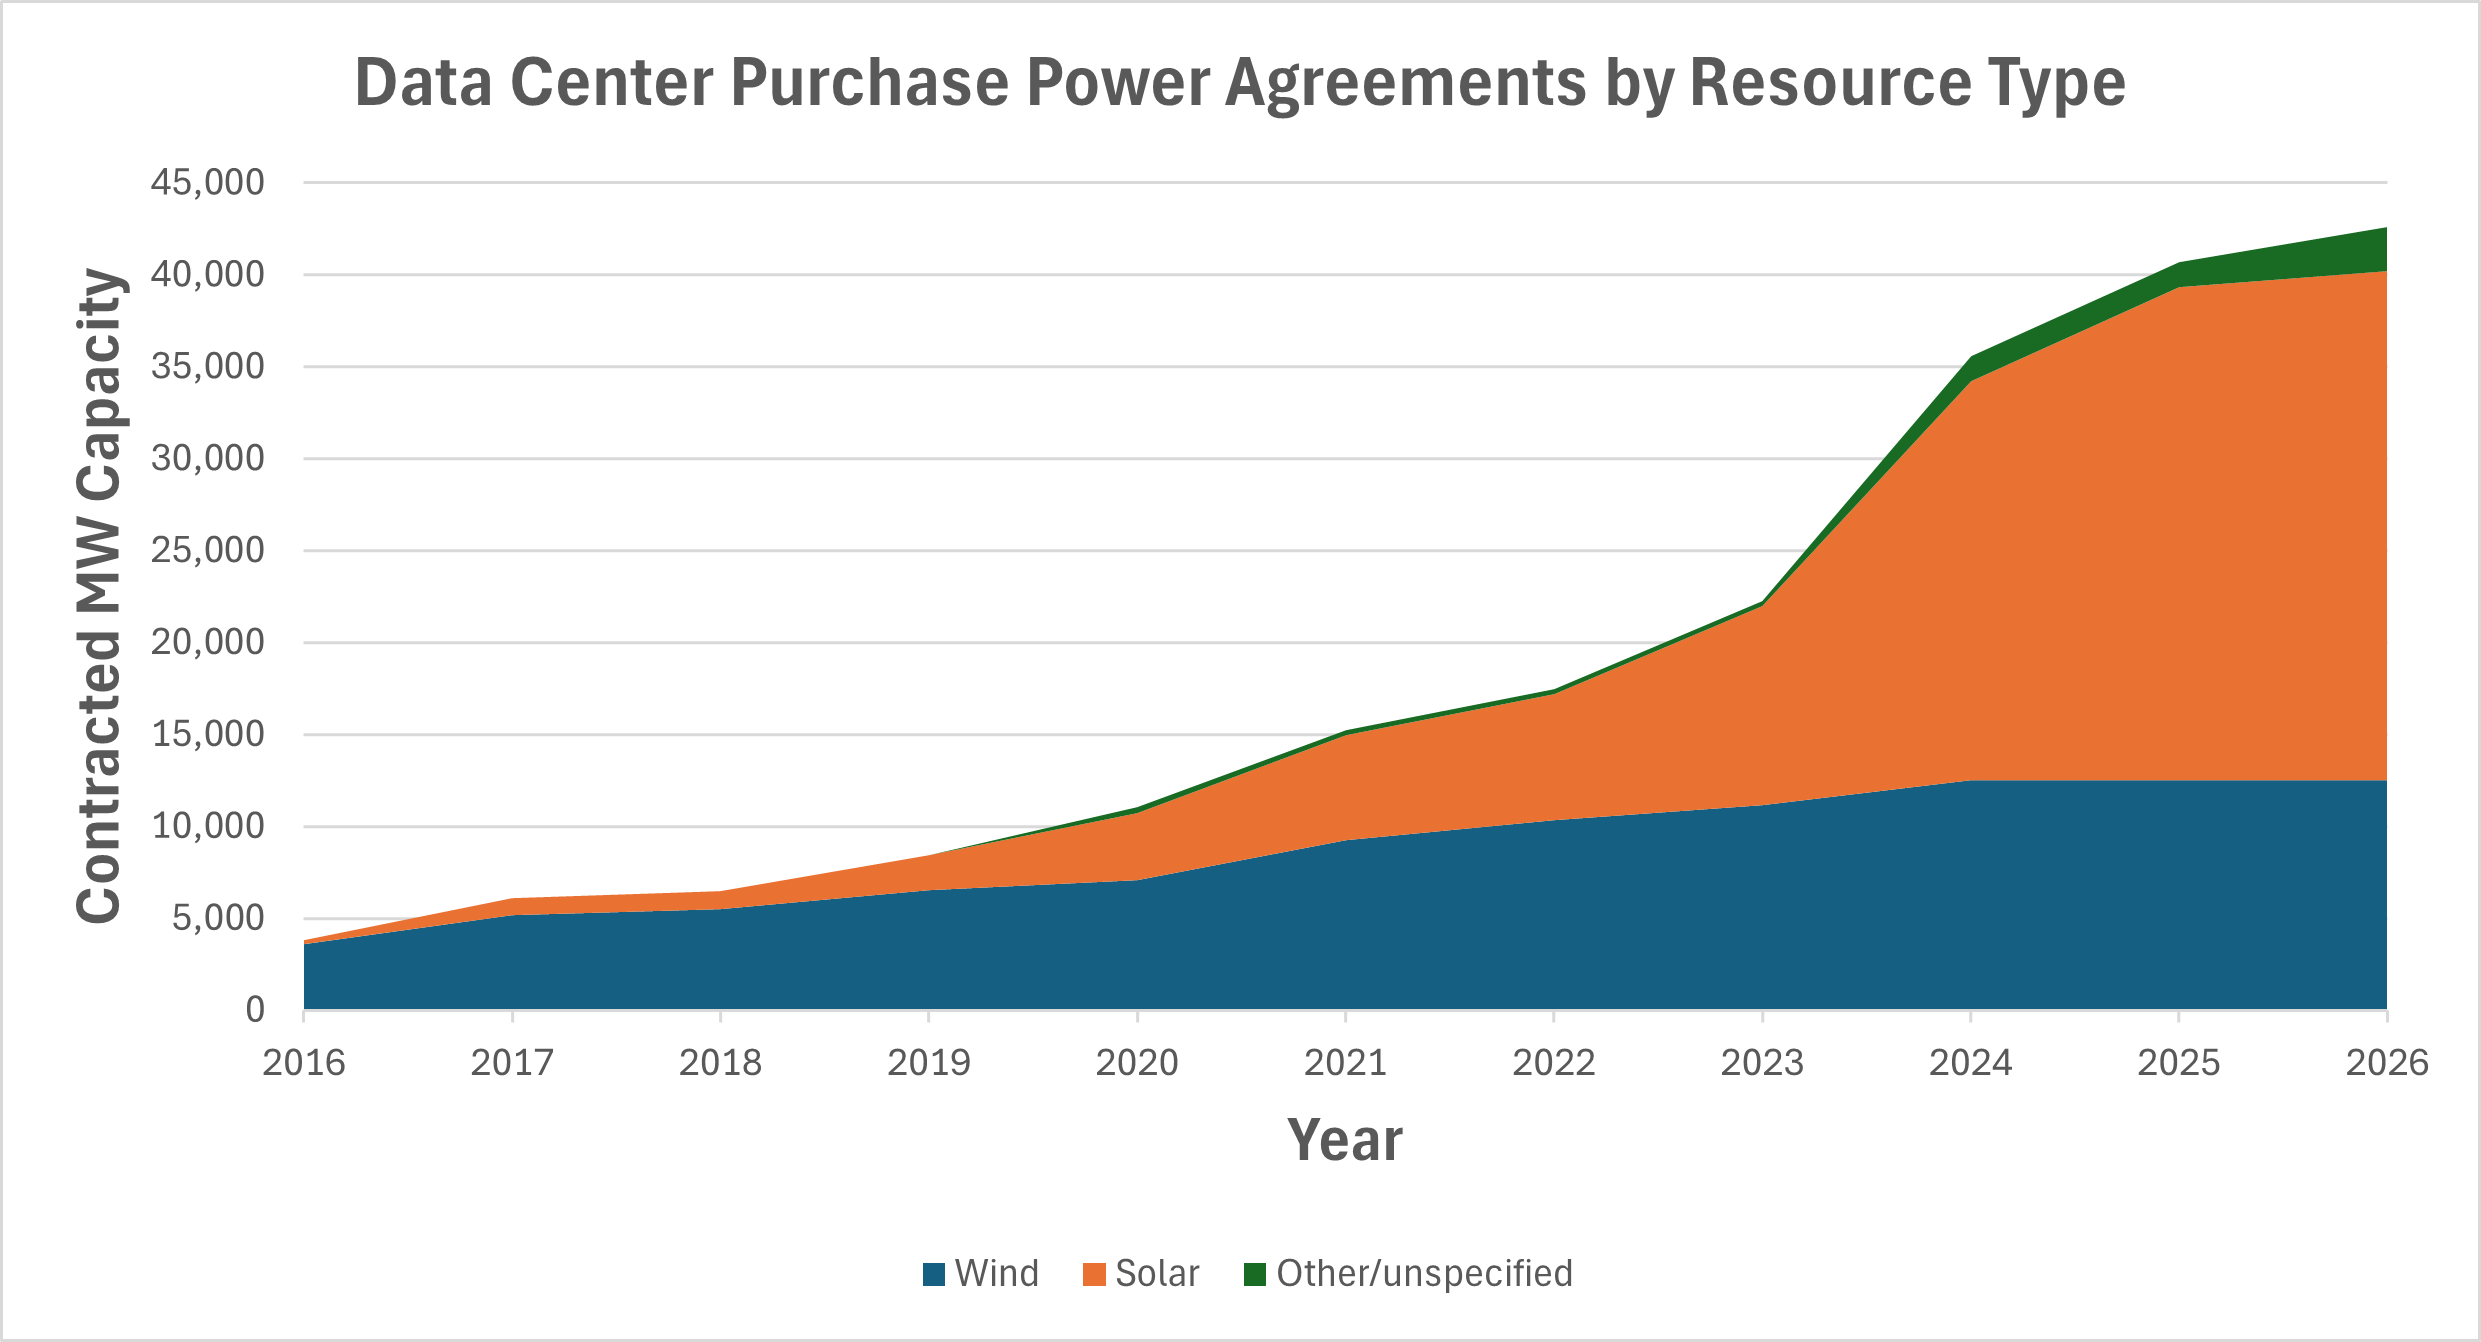
\includegraphics[width=0.5\linewidth]{Figures/PPA by Resource Type.png}
    \caption{PPA agreements by data centers have risen dramatically since 2016.}
    \label{fig:PPAFigure}
\end{figure}

Colocation includes siting dedicated generation at or near a data center, often behind the meter and is increasingly pursued by hyperscale operators. By serving load locally, colocation can reduce transmission congestion and avoid incremental bulk system demand. However, FERC has scrutinized such arrangements for potential cost-shifting to remaining ratepayers, as in the Talen Energy--Amazon arrangement at the Susquehanna nuclear plant \citep{ferc2024_talen_amazon}. The net environmental impact depends on the counterfactual: redirecting generation that would otherwise serve grid load may increase system-wide emissions.

\section{Game Theoretic Model}\label{sec:model}

\subsection{Model}

We present a model of the impacts of varying decision choices for carbon abatement by a large hyperscaler. We present a toy model to illustrate model functioning followed by a full model. We focus on marginal carbon intensity (MCI) and average carbon intensity (ACI). MCI represents the emissions from a particular hour while average carbon intensity represents the total emissions divided by the total generation. While we do not model system-level reliability directly, increases in load without corresponding investments in generation naturally contribute to greater reliability challenges.

\subsection{Toy Model}

\paragraph{Agents and primitives.}
There are two periods $t\in\{1,2\}$ and three generator agents:
a fossil unit $F$, an existing renewable $R_1$, and a potential renewable entrant $R_2$. Figure \ref{fig:Agents} showcases the agents and their interactions with the market.
\begin{figure}[http]
    \centering
    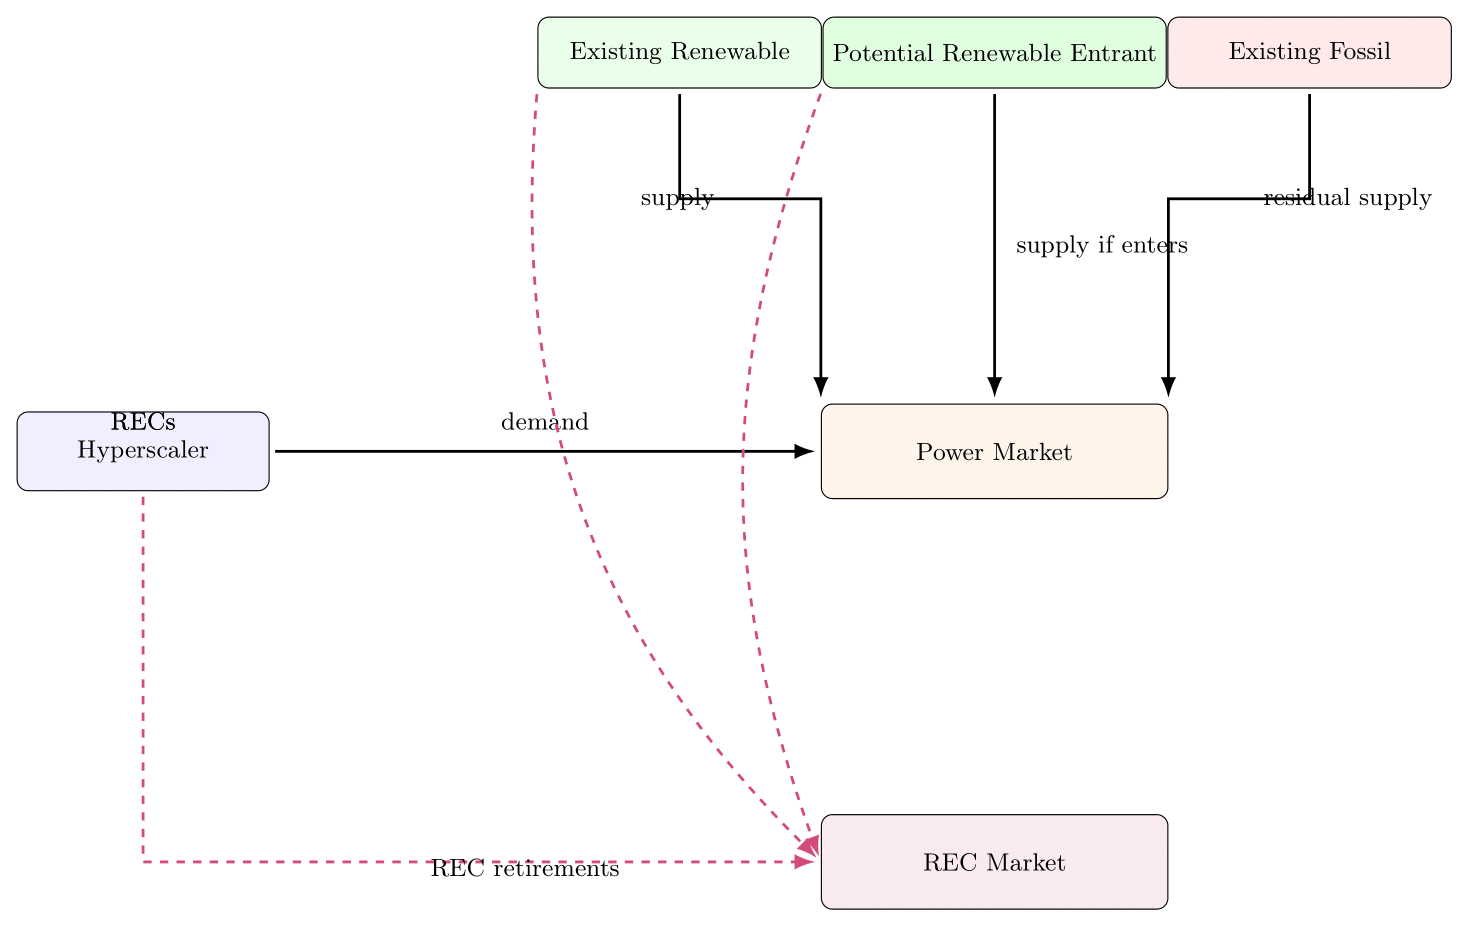
\includegraphics[width=0.5\linewidth]{Figures/Agents-1.png}
    \caption{Agents in Model}
    \label{fig:Agents}
\end{figure}
The hyperscaler has inelastic demand $D^M_t=1$ in each period, and there is no outside demand ($D^O_t=0$).
Variable costs and emissions:
\[
c_F>0,\quad e_F>0,\qquad c_{R_1}=c_{R_2}=0,\quad e_{R_1}=e_{R_2}=0.
\]
Capacities/output (deterministic to highlight timing):
\[
x_{R_1,1}=1,\ \ x_{R_1,2}=0;\qquad x_{R_2,1}=0,\ \ x_{R_2,2}\in\{0,1\};\qquad 
\]
\begin{center}
    $x_{F,t}\in\{0,1\}.$
\end{center}

Renewables are \emph{complementary in time}: $R_1$ only produces in $t=1$, while $R_2$ (if it enters) only produces in $t=2$.
The fossil unit can meet any residual demand.

\paragraph{Dispatch and prices.}
Competitive dispatch follows merit order. If a renewable is available in $t$, it clears the 1~MWh load at $p_t=0$; otherwise $F$ clears at $p_t=c_F$.
Hence, without $R_2$ entry:
\[
p_1=0,\qquad p_2=c_F,\qquad \text{MCI}_1=0,\ \text{MCI}_2=e_F.
\]
With $R_2$ entered, $p_2=0$ as well.

\paragraph{REC mechanics and the timing parameter.}
Each MWh of renewable generates one REC in its production period. Let $S_t$ be REC supply, so without entry $S_1=1$, $S_2=0$; with entry $S_2=1$.
The hyperscaler targets $100\%$ coverage ($\phi=1$) under REC procurement with granularity parameter $h\in[0,1]$:
$h=0$ (annual matching, no timing), $h=1$ (hourly matching).
Let $R^{G}_t$ be granular retirements and $R^{A}$ annual-bucket retirements. Feasibility:
\[
\underbrace{R^G_t \ge h D^M_t}_{\text{granular}},\qquad
\underbrace{R^{A} \ge (1-h)(D^M_1{+}D^M_2)}_{\text{annual}},\qquad
\]

\paragraph{Potential entrant $R_2$.}
If $R_2$ enters, it produces $x_{R_2,2}=1$ in $t=2$. It pays entry cost $I>0$ financed at $1+r(\sigma^2)$.
We compare three procurement environments (which map to different cash-flow risk for $R_2$):
\begin{enumerate}
\item \emph{REC/merchant (no contract).} $R_2$ sells energy at $p_2$ and its REC at $p^{REC}_2$.
\item \emph{PPA.} $R_2$ receives a fixed transfer $\bar p$ per MWh in $t=2$ (energy+REC bundled); residual merchant exposure is zero in this toy case.
\item \emph{Colocation.} $R_2$ is fully contracted on-site at transfer $\tilde p$ per MWh in $t=2$ (no market risk).
\end{enumerate}
We keep discounting trivial (two periods, take $\beta=1$) to focus on timing and entry.

\paragraph{Outcomes by procurement regime.}
\subsection{Full Model}

\paragraph{Agents and primitives.}
We study a market with a large data center hyperscaler (e.g.\ Microsoft) and a set of generators indexed by owner $k$ and technology $l \in \{R,F\}$ (renewable or fossil).\footnote{Index individual plants by $g$ when convenient; technology $l(g)\in\{R,F\}$.} 
The hyperscaler procures electricity to minimize expected total costs by choosing (i) a long-term power supply arrangement $i\in\mathcal I$ and (ii) an emergency backup option $j\in\mathcal J$.

\vspace{0.5em}
\noindent\textbf{Key objects.} 
\begin{itemize}
\item For each generator $g$: capacity $O^{\max}_g$, variable cost $c_g$, emissions rate $e_g$, and stochastic availability.
\item For the hyperscaler: load $\{D^M_t\}_{t=1}^2$, backup option $j\in\{\text{none},\text{diesel},\text{storage}\}$, and procurement $i\in\{\text{REC}, \text{PPA}, \text{Colocation}\}$.
\end{itemize}

\subsection{Timing}

\textbf{Stage 0a (commitment):} The hyperscaler commits to procurement $i\in\mathcal I$ and backup $j\in\mathcal J$ (contract terms public).

\textbf{Stage 0b (entry):} A set of potential generators of both types observes $(i,j)$ and decides whether to enter. Entry costs are sunk upon entry.

\textbf{Stages 1--2 (operations):} In each period $t=1,2$, shocks realize (demand, renewable availability). The energy market dispatches competitively; RECs are issued, banked, and retired subject to granularity rules (the ``timing wedge''). Agents discount with factor $\beta\in(0,1)$ across the two operating periods.

\subsection{Hyperscaler problem (commitment stage)}

The hyperscaler chooses $(i,j)$ to minimize expected total costs:
\begin{equation}
\label{eq:hyper_obj}
\pi_{\text{hyper}} \;=\; \min_{i\in\mathcal I,\, j\in\mathcal J}
\left[
C^{\mathrm{cap}}_i + C^{\mathrm{op}}_i
+ P_{ij}\,C^{\mathrm{out}} + \bar C^{\mathrm{env}}_{ij}
\right],
\end{equation}
where $P_{ij}=P_i P_j$ is the probability that both the contracted source fails and the backup is unavailable, $C^{\mathrm{out}}$ is the outage loss, and $\bar C^{\mathrm{env}}_{ij}=\mathbb{E}[f(\Delta E_{ij})\,C^{\mathrm{env}}_{ij}]$ is the expected reputational cost as a function of the emissions delta $\Delta E_{ij}\equiv E^{\text{with DC}}-E^{\text{without DC}}$.

\paragraph{Contract menu.}
\begin{itemize}
\item \emph{REC/merchant} ($i=\text{REC}$): the hyperscaler buys energy from the grid and retires RECs; generators remain merchant for energy and REC revenue.
\item \emph{PPA} ($i=\text{PPA}$): a renewable generator sells a fixed quantity $\bar q$ each period at price $\bar p$; residual is merchant.
\item \emph{Colocation} ($i=\text{Colo}$): a dedicated renewable unit (optionally with storage) physically colocated with the data center delivers $Q^{\text{colo}}_t$; residual met from the grid. Colocation fully insulates the generator from market risk.
\end{itemize}

\paragraph{Backup.} $j\in\{\text{none},\text{diesel},\text{storage}\}$ affects both reliability ($P_j$) and emissions: diesel has $e_j>0$, storage has $e_j=0$ if charged by colocated renewables.

\subsection{Entry (Stage 0b)}

Potential entrants of type $l\in\{R,F\}$ decide to enter before operations. Let $I_g$ be the sunk entry cost for plant $g$, and let $r(\sigma^2)$ be the project’s financing rate, strictly increasing in the variance of net operating cash flows $\sigma^2$ (a reduced-form cost-of-capital channel). For a renewable merchant entrant,
\begin{equation}
\label{eq:profit_merchant}
\Pi^{R,\text{merch}}_g \;=\; \mathbb{E}\!\left[\sum_{t=1}^{2}\beta^{t-1}\big((p_t+p^{REC}_t) x_{g,t}-c_g x_{g,t}\big) \right]
\;-
\end{equation}
\begin{center}
    $\; I_g\,\Big(1+r(\sigma^2_{\text{merch}})\Big).$
\end{center}
Under a PPA for $\bar q\le O^{\max}_g$ at price $\bar p$,
\begin{equation}
\label{eq:profit_ppa}
\Pi^{R,\text{ppa}}_g \;=\; \sum_{t=1}^{2}\beta^{t-1}\left[\bar p\,\bar q + (p_t+p^{REC}_t)(x_{g,t}-\bar q)_+ - c_g x_{g,t}\right]
\;-
\end{equation}
\begin{center}
    $\; I_g\,\Big(1+r(\sigma^2_{\text{ppa}})\Big).$
\end{center}
Under colocation (full revenue and REC certainty for the contracted amount),
\begin{equation}
\label{eq:profit_colo}
\Pi^{R,\text{colo}}_g \;=\; \sum_{t=1}^{2}\beta^{t-1}\left[\tilde p_t\, Q^{\text{colo}}_t - c_g x_{g,t}\right]
\;-\; I_g\,\Big(1+r(0)\Big),
\end{equation}
where $\tilde p_t$ is the contracted transfer for colocated output. For fossil $F$, replace $(p_t+p^{REC}_t)$ by $p_t$.

\paragraph{Free entry.} With a continuum of potential entrants and competitive supply of projects, free entry implies zero-profit conditions for marginal entrants of each type/contract:
\begin{equation}
\Pi^{l,\cdot}_g \;\le\; 0\quad\text{for all }g,\qquad
\Pi^{l,\cdot}_g=0\ \text{if }g\ \text{enters},\qquad l\in\{R,F\}.
\end{equation}
Because $r(\sigma^2)$ increases in variance and colocation eliminates variance,
\begin{equation}
r(0)\;\le\; r(\sigma^2_{\text{ppa}})\;\le\; r(\sigma^2_{\text{merch}}),
\quad\Rightarrow\quad
\text{entry}_{\text{colo}} \;\ge\;
\end{equation}

\begin{center}
    $\text{entry}_{\text{ppa}} \;\ge\; \text{entry}_{\text{merchant}}
\ \ \text{(all else equal).}$
\end{center}

\subsection{Operations subgame (two periods $t=1,2$)}

\paragraph{Demand.} Total load each period is $D_t=D^M_t+D^O_t$. Net grid draw by the hyperscaler is
\begin{equation}
\label{eq:grid_draw}
G^M_{t} \;=\; \big(D^M_t - Q^{\text{contract}}_{i,t} - Q^{\text{colo}}_t - B_{j,t}\big)_+,
\end{equation}
where $Q^{\text{contract}}_{i,t}$ is the (possibly firm) delivery under $i$ and $B_{j,t}$ is backup output.

\paragraph{Availability.} Each generator $g$ is either fully available or off:
\begin{equation}
x_{g,t}\in\{0,O_g^{\max}\},\quad \Pr(x_{g,t}=O_g^{\max})=\alpha_{g,t}.
\end{equation}

\paragraph{Energy dispatch and price.} Given the set of available units $\mathcal G_t$, the competitive dispatch solves
\begin{equation}
\label{eq:dispatch}
\min_{\{x_{g,t}\}} \ \sum_{g\in\mathcal G_t} c_g x_{g,t} \qquad
\text{s.t.}\quad 
\end{equation}
\begin{center}
    $\sum_{g\in\mathcal G_t} x_{g,t} + B_{j,t} + Q^{\text{colo}}_t \;=\; D_t,\ \ x_{g,t}\in\{0,O_g^{\max}\}.$
\end{center}
Let $\lambda_t$ be the energy balance multiplier. The locational marginal price (LMP) is $p_t=\lambda_t=c_{g^*(t)}$, where $g^*(t)$ is the marginal unit at the optimum.

\paragraph{REC issuance, banking, and the timing wedge.}
Renewables mint one REC per MWh:
\begin{equation}
r_{g,t}=\mathbf 1\{l(g)=R\}\,x_{g,t},\qquad S_t=\sum_g r_{g,t}.
\end{equation}
A stock of banked RECs evolves:
\begin{equation}
\label{eq:bank}
K_{t+1}=(1-\delta)K_t+S_t - R^{\text{ret}}_t,\qquad K_t\in[0,\bar K],\quad t=1,
\end{equation}
with terminal $K_3$ free (or bounded).

To formalize matching granularity, fix a parameter $h\in[0,1]$:
\(h=0\) is annual bucket matching; \(h=1\) is full hour/period matching.
Let $R^{M,G}_t$ be the hyperscaler's \emph{granular} retirements in period $t$
and $R^{M,A}$ its \emph{annual bucket} retirements.
The hyperscaler targets a renewable share $\phi\in[0,1]$ of its total consumption.
Feasibility and obligations:
\begin{align}

\label{eq:gran_req}
&\textbf{(Granular requirement)} 

& R^{M,G}_t \ge h\,\phi\,D^M_t,

&& R^{M,G}_t \ \le\ S^{\text{qual}}_t, \quad t=1,2,\\

\label{eq:annual_req}
&\textbf{(Annual requirement)} & 

R^{M,A} \ \ge\ (1-h)\,\phi\,(D^M_1+D^M_2), \\

&& R^{M,A} \ \le\ K_1+S_1+S_2 - (R^{M,G}_1+R^{M,G}_2),
\end{align}

where $S^{\text{qual}}_t\le S_t$ denotes RECs eligible by geography/tier.
The \emph{timing wedge} is the load not covered by same-period renewable matching:


\begin{equation}
\label{eq:wedge}
w_t(h) \;=\; G^M_t - R^{M,G}_t \ \ \ (\ge 0 \text{ if } h>0 \text{ binds}),
\qquad
\end{equation}

\begin{center}
    $ W(h)=\sum_{t=1}^2 \mathbb{E}[w_t(h)].$
\end{center}

\paragraph{REC market clearing and prices.}
Given banking \eqref{eq:bank} and obligations \eqref{eq:gran_req}--\eqref{eq:annual_req}, the competitive REC allocation minimizes present cost of compliance:
\begin{equation}
\begin{aligned}
\min_{\{R^{\text{ret}}_t,K_2,R^{M,G}_t,R^{M,A}\}} \quad 
& \sum_{t=1}^{2} \beta^{t-1} p^{REC}_t R^{\text{ret}}_t \;+\; \sum_{t=1}^{2} \beta^{t-1} \overline p^{\text{ACP}}_t\, \text{short}_t \\
\text{s.t.}\quad 
& \eqref{eq:bank},\ \eqref{eq:gran_req},\ \eqref{eq:annual_req},\quad
\end{aligned}
\end{equation}
\begin{center}
$R^{\text{ret}}_t = R^{M,G}_t + \mathbf 1\{t=2\}R^{M,A} + R^{\text{LSE}}_t - \text{short}_t,\\
& R^{\cdot}\ge 0,\ \text{short}_t\ge 0.$
\end{center}
Let $\mu$ be the annual-constraint multiplier and $\nu_t$ the granular multipliers.
Then the effective shadow value of a qualifying REC used in $t$ is
\begin{equation}
\label{eq:rec_shadow}
\tilde p^{REC}_t \;=\; p^{REC}_t \;+\; \nu_t \;+\; \mathbf 1\{t=2\}\,\mu.
\end{equation}
With interior banking, the Euler condition implies
\begin{equation}
\label{eq:rec_euler}
p^{REC}_1 \;=\; \beta(1-\delta)\, \mathbb E\left[p^{REC}_2\right],
\end{equation}
and $p^{REC}_t\le\overline p_t^{\text{ACP}}$ with equality if shortfalls occur.

\paragraph{Emissions and carbon intensity.}
Total emissions in $t$ are
\begin{equation}
E_t = \sum_{g\in\mathcal G_t} e_g x_{g,t} + e_j B_{j,t}.
\end{equation}
Define average and marginal carbon intensity:
\begin{equation}
\text{ACI}_t = \frac{E_t}{\sum_g x_{g,t}+B_{j,t}}, 
\qquad \text{MCI}_t = e_{g^*(t)}.
\end{equation}
Microsoft’s attributable marginal emissions under $(i,j)$:
\begin{equation}
\text{MME}_{i,j} \;=\; \sum_{t=1}^2 \beta^{t-1}\,\mathbb E\!\left[\text{MCI}_t \cdot G^M_{t}\right],
\end{equation}
with $G^M_t$ in \eqref{eq:grid_draw}.

\subsubsection{Equilibrium}

Given $(i,j)$ and the set of entrants from Stage 0b, a \emph{competitive two-period operating equilibrium} is a tuple 
\[
\big\{\{x_{g,t}\}, \{p_t\}, \{p^{REC}_t\}, K_2, \{R^{M,G}_t\}, R^{M,A}\big\}_{t=1,2}
\]
such that (i) dispatch \eqref{eq:dispatch} clears energy with $p_t=c_{g^*(t)}$; (ii) REC issuance/banking/retirements satisfy \eqref{eq:bank}, \eqref{eq:gran_req}--\eqref{eq:annual_req}, and REC prices satisfy \eqref{eq:rec_euler}; and (iii) backup and colocation quantities meet \eqref{eq:grid_draw}. A \emph{subgame-perfect equilibrium} of the full game consists of $(i^*,j^*)$ solving \eqref{eq:hyper_obj}, a set of entrants satisfying free-entry conditions, and a competitive operating equilibrium in each period.


\subsubsection{Mechanisms and Equilibrium Implications}

Three mechanisms drive outcomes. First, procurement choices shape operational emissions through the
\emph{timing wedge} between load and renewable generation. Colocation with storage shrinks this wedge by re-timing renewable energy into high-carbon hours; diesel backup increases emissions. 

Second, contract type alters financing risk: PPAs reduce $\sigma^2$ relative to RECs, and colocation eliminates it. Lower variance reduces $r(\sigma^2)$, encouraging renewable entry. 

Third, equilibrium carbon intensity reflects both the short-run operational effect and the long-run investment effect. 

\subsubsection{Implications}

Our model provides a set of empirical predictions about how hyperscalers’ procurement choices affect both costs and carbon intensity. On the demand side, as the spread between the cost of procuring electricity from renewable sources and from the open market widens, hyperscalers are more likely to turn to the open market and less likely to contract renewables. At the same time, as hyperscaler demand for electricity grows, the environmental cost of their consumption rises, and the benefits of carbon-free procurement mechanisms such as PPAs and colocation increase. These benefits scale with both the overall carbon intensity of grid electricity and the size of the hyperscaler’s load: the dirtier and larger the load, the greater the incentive to secure clean and reputationally valuable supply.

On the supply side, the model emphasizes that because renewable generation is intermittent, incremental data center demand tends to raise fossil generation unless there is sufficient storage to shift renewable energy across periods. The timing mismatch between hyperscaler load and renewable output—the “timing wedge”—is therefore central to understanding operational emissions outcomes. Colocation with storage can shrink this wedge by re-timing renewable production to high-carbon hours, while diesel backup increases emissions during outages.

These mechanics give rise to several testable implications. First, REC purchases on their own do not alter short-run carbon intensity, since they are purely financial transfers. Their effect arises only in the medium run, if REC demand raises REC prices and induces new renewable capacity to come online. PPAs without firming behave similarly in operational terms, but they reduce generators’ revenue risk and financing costs, which increases renewable entry relative to REC-only arrangements. Colocation has a more immediate impact: behind-the-meter renewable output reduces a hyperscaler’s net grid draw exactly when the colocated plant is producing, lowering local marginal emissions exposure. The effect is strongest when renewable output is correlated with hyperscaler load. Adding storage to colocation further enhances this benefit by shifting surplus renewable production to periods when demand is high and marginal carbon intensity is greatest, sharply reducing emissions attributable to the data center. This also can an emissions effect as the reduced timing wedge better matches power, and the behind-the-meter power can add resilience to the grid. By contrast, reliance on diesel backup increases operational emissions whenever it is deployed.

Finally, the model predicts an investment hierarchy driven by financing risk: colocation, by fully eliminating revenue variance, induces the largest increase in renewable entry, followed by PPAs, and then REC purchases. This creates a long-run ordering in expected carbon reductions. Moreover, because colocated renewables reduce grid purchases at the hyperscaler’s node, emissions fall locally, though congestion and flow adjustments may increase carbon intensity in neighboring nodes unless total renewable capacity expands.

Together, these predictions imply that (i) REC purchases yield little immediate emissions reduction but may encourage new renewable entry; (ii) PPAs accelerate renewable deployment by reducing financing risk, though without firming they do not improve operational carbon intensity in the short run; and (iii) colocation—especially when paired with storage—directly lowers hyperscaler-attributable emissions by addressing the timing wedge between renewable generation and hyperscaler demand.

\section{Empirical Overview}\label{Sec::Methods}

We estimate the causal effect of AI workloads on four outcomes in wholesale electricity markets: local power quality, fossil fuel demand, wholesale prices, and the differential response across training versus inference phases. The central identification problem is that the objects of interest such as the timing, location, and intensity of compute activity at individual data centers, are proprietary. We observe neither training start dates nor facility-level load; instead, we observe publicly announced model release dates, the geographic footprint of hyperscaler data centers, and zonal market outcomes. Our strategy exploits model releases as the observable shock and uses difference-in-differences to recover treatment effects from the remaining variation.

\subsection{Identification}\label{EconometricModel}

Let $Y_{it}$ denote an outcome (power quality, fossil generation, or price) for zone $i$ in period $t$, and let model release $m$ occur at date $r_m$. Zones linked to the releasing firm's data center footprint constitute the treated group for event $m$; zones without exposure to that firm's AI activity in the event window form the control group. Under the standard parallel-trends and no-anticipation assumptions, differencing outcomes across treated and control zones before and after $r_m$ identifies the average treatment effect on the treated. Because our outcomes, wholesale prices, fossil generation, voltage distortion, are transmitted through markets and the physical grid rather than through proprietary firm-level data, this approach follows a long tradition of recovering unobservable inputs from observable market equilibria \citep{fowlie2012industrial, card1994minimum, greenstone2014environmental}.

Four features of our setting complicate a textbook two-period DiD. First, training windows are unobserved: we know when a model was released but not when its training began, so the ``treatment date'' is imprecise. Second, releases are staggered across firms and calendar time, which under treatment-effect heterogeneity causes two-way fixed effects estimators to weight already-treated units as implicit controls for later-treated units \citep{goodman2021difference, sun2021treatment, callaway2021difference, borusyak2024revisiting}. Third, parallel trends is not innocuous in electricity markets, where fuel prices, weather, and secular load growth move outcomes in ways potentially correlated with data center siting. Fourth, treatment exposure itself must be constructed: no dataset directly links model releases to zonal load, and assigning generators and facilities to market zones requires substantial preprocessing (see Appendix \ref{zonalMappingEfforts}).

We address the first two issues with a stacked event-study design that anchors treatment on observed release dates and builds clean control groups for each release cohort, developed in Section \ref{subsec:eventstudy}. We address the third through pre-trend tests, placebo exercises, and controls for fuel costs, temperature, and renewable output (Section \ref{Robustness}). The fourth is resolved in our data construction, described in Section \ref{sectionData}.

\section{Estimation Strategy}\label{sec:empirical}

To address the inexact information about training windows and release times, we estimate dynamic treatment effects at multiple horizons relative to model release dates. This approach, referred to as an event study or \textbf{stacked difference-in-differences} in econometrics, offers three advantages over the standard pre/post comparison discussed earlier: (1) it does not require observing the true training start date, instead using release timing as the anchor; (2) it also provides a direct test of the parallel trends assumption through examination of pre-release coefficients; and (3) it allows the data to reveal the temporal profile of effects rather than imposing an arbitrary discontinuous treatment structure.

\subsection{Stacked DiD with Multiple Horizons}%Event-Study Framework}
\label{subsec:eventstudy}
Formally, we define treatment exposure relative to each model's release date $r_m$ for both training and release: \textbf{1) Training windows:} The period $[r_m - \bar{\tau}_{\text{train}}, r_m)$ preceding release, during which computational resources are devoted to model training. We remain agnostic about the exact training start date; our identifying assumption is that training activity is elevated in the months before release and that any pre-existing differential trends would manifest in the earlier leads. \textbf{2) Inference window:} The period $[r_m, r_m + \bar{\tau}_{\text{infer}}]$ following release, during which the model is deployed for inference via API access or public availability.


\subsubsection{Stacked Difference-in-Difference}

Model releases occur at different calendar dates, creating a staggered adoption setting. Recent econometric literature has demonstrated that conventional two-way fixed effects (TWFE) estimators as is the case in the estimates from traditional difference-in-differences. 
can produce biased estimates under treatment effect heterogeneity 
\cite{goodman2021difference, sun2021treatment, callaway2021difference, borusyak2024revisiting}. Treatment effect heterogeneity means the policy works differently for different places or periods, which can distort standard difference-in-differences estimates. The bias arises because TWFE implicitly uses already-treated units as controls for later-treated units, and differences in treatment effects across cohorts or over time contaminate the estimated average effect. 

In our setting, consider regions as units and AI model releases as treatments inducing increased data center power demand. A ``cohort" comprises regions whose data centers began significant AI workloads at the same time. Suppose Region A adopted AI workloads in 2022 while Region B adopted in 2023. When estimating treatment effects for Region B, TWFE implicitly uses Region A as a control—but Region A in 2023 is not untreated; its data centers have been running AI workloads for a year. If treatment effects evolve over time (e.g., power demand grows as AI infrastructure scales), comparing Region B's outcomes against Region A's already-treated outcomes introduces bias. Staggered design provides heterogeneity-robust estimators that solve for this exact issue.

%\nb{Can you explain the previous sentence in terms of data centers and time wrt power demand? It is hard to know what already-treated, later-treated units, cohorts etc mean.}

To address this, we use a stacked DiD model~\cite{cengiz2019effect, deshpande2019screened}, where we construct a stacked dataset where each model release defines a separate ``sub-experiment.'' The idea here is to construct, for each treatment cohort, a separate sub-experiment using only units that are genuinely untreated at the time of that cohort's adoption. By stacking these sub-experiments—each with its own clean control group of not-yet-treated regions—we ensure that no already-treated unit ever serves as a control, thereby eliminating the bias that arises when treatment effects are heterogeneous across cohorts or time.

Formally, for each release event $m$, we create a dataset containing: (i) Treated units -- Regions linked to the releasing company's AI data centers. (ii) Control units -- Regions with no AI data center exposure during the event window, or regions whose treatment occurs sufficiently far from event $m$ that they serve as clean controls.
\begin{itemize}
    \item Time window: A symmetric window around $r_m$, e.g., $[r_m - K, r_m + K]$ for some horizon $K$.
\end{itemize}

Following \cite{wing2024stacked}, we then stack these sub-experiments and estimate:
\begin{equation}
Y_{i,t,m} = \sum_{k=-K}^{K} \beta_k \cdot D_{ut}^k  + \delta_t + \mathbf{X}_{ut}'\theta + \varepsilon_{ut}
\label{eq:stacked}
\end{equation}
where $\gamma_{u}$ are unit-by-event fixed effects, $\delta_{u}$ are time-by-event fixed effects, $\mathbf{X}_{ut}'\theta$ represents controls, and the coefficients $\{\beta_k\}$ trace out the dynamic treatment effect at each event-time horizon $k$. Standard errors are clustered at the unit level to account for correlation across events within the same region.


\subsection{Estimating Power Quality}

Our power quality analysis estimates the following stacked DiD specification at the utility-month level:
\begin{equation}
\text{PowerQuality}_{ut} = \sum_{k=-K}^{K} \beta_k^{PQ} \cdot D_{ut}^k + \gamma_u + \delta_t + \mathbf{X}_{ut}'\theta + \varepsilon_{ut}
\label{eq:pq_eventstudy}
\end{equation}
where:
\begin{itemize}
    \item $\text{PowerQuality}_{ut}$ is the Whisker Labs Consumer Power Quality Index for utility $u$ in month $t$;
    \item $D_{ut}^k = \mathbf{1}[\text{event-time} = k] \times \text{Treated}_u$ indicates that utility $u$ is $k$ periods from the release date of a model linked to an AI data center in its service territory;
    \item $\gamma_u$ are utility fixed effects absorbing time-invariant characteristics;
    \item $\delta_t$ are calendar month fixed effects absorbing common temporal shocks;
    \item $\mathbf{X}_{ut}$ includes time-varying controls (weather, regional load).
\end{itemize}

We estimate an analogous specification for total harmonic distortion (THD):
\begin{equation}
\text{THD}_{ut} = \sum_{k=-K}^{K} \beta_k^{THD} \cdot D_{ut}^k + \gamma_u + \delta_t + \mathbf{X}_{ut}'\theta + \varepsilon_{ut}
\label{eq:thd_eventstudy}
\end{equation}

% \paragraph{Identifying Assumption.} \nb{Arent we moving this to 3.5 or 3.6?} The key identifying assumption is that, absent the AI model release, treated and control utilities would have followed parallel trends in power quality. We assess this assumption by examining the estimated coefficients $\{\beta_k : k < 0\}$ in the pre-release period. Under parallel trends, these coefficients should be statistically indistinguishable from zero. Systematic pre-trends would indicate either (a) anticipatory effects, (b) confounding from correlated unobservables, or (c) differential trends predating treatment.

\subsection{Estimating Fossil Fuel Demand}

Power demand analysis proceeds at the generator-month level, exploiting finer geographic resolution. We maintain the stacked DiD structure while incorporating instrumental variables to address the price endogeneity concern:

\paragraph{First Stage.} We instrument for electricity prices using supply-side cost shifters:
\begin{equation}
p_{it} = \pi_0 + \pi_1 \text{HeatRate}_{it} + \pi_2 \text{GasPrice}_{t} + \gamma_i + \delta_t + \mathbf{X}_{it}'\pi_3 + \nu_{it}
\label{eq:firststage}
\end{equation}
where $\text{HeatRate}_{it}$ captures the thermal efficiency of generator $i$ and $\text{GasPrice}_t$ is the contemporaneous natural gas spot price. These instruments satisfy relevance (they are primary determinants of marginal generation costs) and exclusion (they affect demand only through their impact on prices, not through direct effects on AI workload scheduling or other consumption decisions).

\paragraph{Second Stage.} We estimate the stacked DiD specification using predicted prices:
\begin{equation}
\text{FossilDemand}_{it} = \sum_{k=-K}^{K} \beta_k^{FD} \cdot D_{it}^k + \eta \hat{p}_{it} + \gamma_i + \delta_t + \mathbf{X}_{it}'\theta + \varepsilon_{it}
\label{eq:demand_eventstudy}
\end{equation}
where $D_{it}^k$ indicates event-time relative to model releases linked to AI data centers in generator $i$'s service area.

The coefficients $\{\beta_k^{FD}\}$ capture the dynamic effect of AI activity on fossil fuel demand. Negative values of $k$ (pre-release) correspond to the training phase; positive values correspond to inference. The price coefficient $\eta$ controls for supply-driven price movements and provides a scaling factor for welfare calculations. Difference between samples in our main analyses are highlighted in the Appendix in Subsection \ref{subsec:differences}.

%\niranjan{Mention how the data is used to learn/estimate the co-efficients.}
%\niranjan{Add an equation here and refer to it in the text above.}

% \end{figure}
% \subsection{Empirical Strategy Details}
% This section presents our identification strategy for estimating the causal effects of AI model development on electricity grid outcomes. We analyze two primary outcomes: (1) power quality degradation at the utility level, and (2) fossil fuel generation demand at the generator level. Our approach employs an event-study framework centered on AI model release dates, with distinct treatment windows corresponding to the training and inference phases of AI development. We address identification challenges arising from staggered treatment timing, data limitations in linking models to specific training locations, and potential violations of parallel trends.



\subsection{Estimating Price Effects}\label{PriceEffects}
% \nb{Make this more explanatory for someone who knows almost nothing about supply/demand and their relationships.}
Beyond quantity effects, we estimate how AI-driven demand increases affect electricity prices. The key economic insight is that price impacts depend on supply flexibility: when generators can easily expand output, demand increases are absorbed with minimal price changes, but when supply is constrained, demand shocks translate primarily into higher prices. The supply elasticity $\varepsilon^s$—the percentage change in quantity supplied per one percent price change—quantifies this responsiveness.

Our estimation proceeds in two steps. First, we use our IV estimates to quantify how AI activity shifts demand:
\begin{equation}
\Delta \widehat{\text{FossilDemand}}{it} = \hat{\beta} \cdot \Delta \text{AI}{it}
\label{eq:demand-change}
\end{equation}

Second, we trace this shift through the supply curve. With linear supply $Q^s=a+b\cdot p_i$, the price change is $\Delta p=\hat{\beta}\cdot \frac{\Delta AI_{it}}{b}$, or in elasticity form:

\begin{equation}
\% \Delta p = \frac{\% \Delta Q^d}{\varepsilon^s}
\label{eq:price-impact-elasticity}
\end{equation}

We estimate $\varepsilon^s$ via IV regression of quantity on price in log-log form, using demand-side instruments (weather-driven load variation and industrial production indices).

We focus on PJM at the zonal level for this analysis. We restrict to a single ISO because differing market structures make prices incomparable across ISOs, and choose PJM because it is the largest (65 million people, 13 states), includes key data center states (Virginia, Pennsylvania), and provides 20 diverse pricing zones. Because observed training locations are outside PJM, this analysis uses the broader model set only.
% \paragraph{Demand Change from Treatment Effect.} The estimated coefficient $\hat{\beta}$ gives the predicted demand change for a given change in AI activity:
% \begin{equation}
% \Delta \widehat{\text{FossilDemand}}_{it} = \hat{\beta} \cdot \Delta \text{AI}_{it}
% \label{eq:demand-change}
% \end{equation}

% \paragraph{Price Impact via Supply Elasticity.} A demand shift $\Delta Q^d$ yields a price change determined by supply responsiveness. With linear supply $Q^s = a + b \cdot p$:
% \begin{equation}
% \Delta p = \frac{\hat{\beta} \cdot \Delta \text{AI}_{it}}{b}
% \label{eq:price-impact}
% \end{equation}
% In elasticity form, for a percentage demand increase $\% \Delta Q^d$:
% \begin{equation}
% \% \Delta p = \frac{\% \Delta Q^d}{\varepsilon^s}
% \label{eq:price-impact-elasticity}
% \end{equation}
% We estimate $\varepsilon^s$ via two-stage IV regression of quantity on price in log-log form, using demand-side instruments (weather-driven load variation and industrial production indices) rather than supply-side instruments. We then combine this elasticity estimate with the demand shift from earlier regressions to calculate price impact. For specifically this regression, we focus on the Independent System Operator (ISO) PJM at a zonal level. We choose to focus on one ISO because differently structured capacity markets and differing market structures mean that prices are not truly equivalent across ISOs. We focus specifically on PJM because it is the largest ISO by population including 65 million people over 13 states and crucially includes Virginia and Pennsylvania, two of the main data center hotbeds. PJM also has 20 diverse zones providing the neccecary granularity. Because the observed training locations are not in PJM, this analysis can only be conducted with the broader model set and not our conservative main analysis.
% \begin{center}
% \textit{[PLACEHOLDER: Table of models with verified training start dates, training end dates, and API/inference release dates from public announcements, papers, or regulatory filings]}
% \end{center}

\section{Validating Assumptions and Robustness}
\label{subsec:robustness}

We implement several diagnostic and robustness exercises to assess the credibility of our estimates.

\subsubsection{Sample Selection}

Our empirical strategy balances internal validity with external relevance. Our main sample comprises four models for which we observe exact training and inference dates as well as training location, and we employ propensity score matching (described in the appendix) to support the parallel trends assumption. We then report results for progressively larger samples of models and data centers, accepting weaker identification in exchange for broader coverage. This approach enables precise, well-identified estimates from our core sample while exploring heterogeneity and counterfactuals in extended samples, with appropriate caveats regarding the latter.

% We vary our sample, so we can provide highly robust estimates of treatment effects using a sample we have exceptional information about while exploring observed heterogeneity in larger samples to enable interesting analysis and counterfactual. We demonstrate robustness for the samples that are less controlled. In our main sample, we focus on four models for which we know exact training and inference dates as well as the location of training. We also utilize propensity score matching as described in the appendix in order to ensure the satisfaction of the parallel trends assumption. We report results for alternative progressively larger samples of models and datacenter with fewer robustness protections to provide a fuller picture with the caveat that less confidence exists in the estimated results. We feel that this conservative approach both allows us to make specific and measured statements and also broader but more impactful statements.

\subsubsection{Pre-Trends and Parallel Trends Testing}

Our primary test of the identifying assumption examines whether pre-release coefficients $\{\beta_k : k < 0\}$ are jointly indistinguishable from zero. We report:
\begin{itemize}
    \item Point estimates and confidence intervals for each lead coefficient.
    \item An F-test of the joint null hypothesis $H_0: \beta_{-K} = \beta_{-K+1} = \cdots = \beta_{-1} = 0$.
\end{itemize}
Significant pre-trends would undermine the causal interpretation of post-release estimates.

\subsubsection{Placebo Tests with Randomized Treatment Assignment}

To verify that our estimates reflect genuine treatment effects rather than spurious correlations or specification artifacts, we conduct placebo tests with randomly assigned treatment:
\begin{enumerate}
    \item \textbf{Random treatment timing:} We hold the set of treated units fixed but randomly reassign release dates drawn from the empirical distribution of actual release dates. Under the null of no effect, placebo estimates should center on zero.
    \item \textbf{Random treatment assignment:} We hold release timing fixed but randomly reassign treatment status across units. This tests whether results are driven by the specific geographic pattern of AI data center locations.
\end{enumerate}
% For each placebo design, we generate five draws and compare our actual estimates to the distribution of placebo estimates. We report the share of placebo estimates exceeding our point estimate in absolute value (a randomization inference p-value).

% \nb{Dana, add some text that says how this relates to the paragraph above?}
\subsubsection{Callaway-Sant'Anna Estimator}
% \paragraph{.} \nb{Can we move the robustness checks etc to 3.6?} 
%\nb{This requires some glue text to explain what issue this is addressing}

As a robustness check and to provide transparent decomposition of treatment effect heterogeneity, we also implement the \citet{callaway2021difference} estimator. Like the stacked approach, CS avoids using already-treated units as controls; however, rather than achieving this through sample construction, it does so by estimating separate ATT(g,t) parameters for each cohort g and time period t, then aggregating these to form summary measures. This approach explicitly avoids problematic comparisons and provides a framework for testing parallel trends through examination of pre-treatment ATT(g,t) estimates. 
\subsubsection{Time-Series Anomaly Detection}

As an internal consistency check, we apply time-series anomaly detection methods to the outcome variables in treated units. If AI model releases causally affect grid outcomes, we should observe detected anomalies clustering around treatment dates. Specifically:
\begin{enumerate}
    \item For each treated unit, we fit a baseline time-series seasonal ARIMA model to the pre-treatment period.
    \item We generate one-step-ahead forecasts and prediction intervals for the post-treatment period.
    \item We flag observations where realized values fall outside the 20\% prediction interval as anomalies.
    \item We test whether anomaly frequency is elevated in the post-treatment window relative to the pre-treatment window and relative to control units.
\end{enumerate}
This approach provides model-free evidence of structural breaks coinciding with treatment timing.

\subsubsection{Sensitivity to Treatment Definition}

Given uncertainty in linking models to specific training locations, we assess robustness to alternative treatment definitions in our less conservative analysis version:
\begin{enumerate}
    \item \textbf{Intensive margin:} Weight treatment by the number or capacity of AI data centers in the region, rather than using a binary indicator.
    \item \textbf{Dropping ambiguous cases:} Exclude model releases where the company operates data centers in multiple balancing authorities, restricting to cases with cleaner geographic attribution.
    \item \textbf{Verified timing subset:} Estimate separately on the subset of models with externally verified training windows.
    \item \textbf{Geographic Resolution and Robustness.} The generator-level data permit more granular treatment definitions than the utility-level power quality data. We exploit this flexibility by estimating specifications under alternative treatment definitions in terms of radius.
\end{enumerate}

\subsubsection{Heterogeneity by Model Characteristics}

We examine whether treatment effects vary with observable model characteristics:
\begin{itemize}
    \item Model scale (parameter count, reported compute).
    \item Company (to assess whether effects are driven by specific firms).
    \item Release year (to assess whether effects are changing over time).
\end{itemize}
Heterogeneity analysis both informs mechanisms and serves as a specification check: if effects are concentrated among larger models or models from companies with substantial AI infrastructure, this lends credibility to the AI-driven interpretation.
\subsection{Counterfactual Analysis}\label{counterfactuals}%Efficiency Impact Model}\niranjan{Compress}

We conduct three primary sets of counterfactual exercises to investigate how alternative evolutionary paths for AI compute might affect grid-level outcomes. Additional counterfactuals with results are highlighted in Appendix Subsection \ref{Appendix:Counterfactuals}.

\textbf{Model Scaling.} First, we examine the grid implications of continued growth in AI model size. Using the Epoch database to characterize trends in model parameters, we provide descriptive analysis of how increasing model scale translates into grid-level impacts. We then relate our estimated power demand coefficients to our power quality coefficients, enabling analysis of how changes in training and inference energy efficiency propagate to power quality outcomes.

\textbf{Geographic Redistribution.} Second, we leverage the geographic locations of data centers in conjunction with our econometric estimates to conduct counterfactuals focused on spatial reallocation of AI compute. We consider two scenarios. In the first, we simulate a shift from cloud-based to edge-based inference—reallocating inference demand from concentrated hyperscaler facilities to smaller data centers distributed closer to population centers. We implement this by redistributing our estimated inference demand impacts across data centers not currently classified as AI-focused. In the second scenario, we simulate relocating training workloads from population-dense regions on the East Coast to energy-abundant regions in the center of the country. For both geographic counterfactuals, we provide sensitivity analyses in the appendix to account for potential increases in communication costs and efficiency losses.

\textbf{Colocated on-site Power Generation.} Finally, we exploit a new feature in the Aterio data, namely a flag on data centers with on-site power generation. We re-estimate both our main models separately for generators with and generators without onsite power generation. We then report the impacts to power demand and power quality of either removing all onsite generation or having onsite generation for all data centers.


Together, these counterfactuals illuminate both how the grid might be affected by different trajectories for AI compute and which levers—geographic placement, workload composition, efficiency improvements—may be available to computer scientists and policymakers seeking to mitigate grid impacts.
%\niranjan{The main idea is to design regressors that can tell us how changes in efficiency e.g., reduction in model parameters, impacts power quality and demand. Note we already have a model for how the power quality changes for a certain set of AI model releases. We can use this to .... To do this we need... }

%Our methodology combines econometric estimates with data from the Epoch database on the number of parameters of models as well as estimates of the impacts of increasing model parameters on relative energy usage. We perform regressions on our coefficients on training compute FLOPS and parameters. This allows us to determine how relative increases in the model's efficiency can lead to changes in model power demand and quality.

%We also perform a techno-economic analysis of the impacts of increasing model size and the number of simultaneous GPUs on energy consumption. This analysis combines econometric estimates with experimental evidence we generated by training a subset of smaller models under different GPU counts and sizes, allowing us to directly observe the contribution of message passing between GPUs to total training energy costs. We essentially extrapolate our experimental results to larger production-level models to estimate the real-world impact of the power reductions from the experiments. Together, these approaches provide a framework for translating trends in AI model scaling into counterfactual grid-level impacts.

% We also run a difference-in-difference regression of the entire length of the interconnection queue and the length of the interconnection queue specifically for natural gas for counties before and after the announcement of a major data center.

% \begin{equation*}
% \text{TotalQueue}_{ct} = \alpha' 
% + \beta' \left( \text{Post}_{t} \times \text{Treatment}_{c} \right)
% + \gamma'_c + \delta'_t + \varepsilon'_{ct}
% \end{equation*}

% \begin{equation*}
% \text{GasQueue}_{ct} = \alpha 
% + \beta \left( \text{Post}_{t} \times \text{Treatment}_{c} \right)
% + \gamma_c + \delta_t + \varepsilon_{ct}
% \end{equation*}

% We also interact the capacity and square footage of the data center with the variable for after the data center's implementation to determine the impact of a MW of capacity from data centers on the interconnection queue. This provides an understanding of how natural gas investments increase following data center announcements and provides evidence for how data centers impact capacity investments.

% \begin{equation*}
%     \text{GasQueue}_{ct} = \alpha + \beta_1 \left( \text{Post}_{t} \times \text{Capacity}_{c} \right)+ \gamma_c + \delta_t + \varepsilon_{ct}
% \end{equation*}

% \begin{equation*}
%     \text{GasQueue}_{ct} = \alpha + \beta_2 \left( \text{Post}_{t} \times \text{SqFt}_{c} \right)+ \gamma_c + \delta_t + \varepsilon_{ct}
% \end{equation*}

% In order to consider the impacts of PPAs by data centers, we look at EIA form 860 data on capacity investments in counties with data centers as well as counties with PPAs by tech companies. PPA data comes from S\& P Capital IQ Pro and is used to perform difference-in-differences regressions of entry capacity of renewable resources on power purchase agreements. We further perform a similar regression of capacity investments in natural gas on announcements of data centers to determine whether PPAs are leading to more renewable or fossil fuel capacity additions.

% % 1. Renewable capacity entry and PPAs
% \begin{equation}
% \text{RenewCap}_{ct} 
% = \alpha 
% + \beta \, (\text{PPA}_c \times \text{Post}_t) 
% + \gamma_c + \delta_t 
% + \varepsilon_{ct}
% \end{equation}

% % 2. Fossil (natural gas) capacity entry and data center announcements
% \begin{equation}
% \text{GasCap}_{ct} 
% = \alpha 
% + \theta \, (\text{DCAnnounce}_c \times \text{Post}_t) 
% + \gamma_c + \delta_t 
% + \varepsilon_{ct}
% \end{equation}

% \subsection{Controls}
% \aruna{Not clear if we need this section given we discuss the controls in each of the specific section, thoughts?}
% The difference-in-differences framework relies on the assumption that, absent treatment, outcomes for treated and control groups would have evolved along parallel trends. Potential threats to this assumption include \emph{group-specific shocks} such as local infrastructure upgrades or outages that disproportionately affect power quality, \emph{anticipation effects} including preemptive grid adjustments ahead of a model release, and \emph{spillovers} like load shifting from nearby control regions. Any of these could bias estimated treatment effects if not properly accounted for. To mitigate these risks, we incorporate controls for weather and fuel prices, as well as geographic and temporal fixed effects. For instance, we explicitly model the impacts of weather conditions by including weather control variables to ensure that systematic climatic variation—which could influence both electricity demand and grid stability—does not confound our estimates.


\section{Data}\label{sectionData}
%\niranjan{To address the three questions we need the following data -- refer to data about variables of interest, control data}
%\niranjan{What we have now is the data of this kind. Who publishes it ... We combine these sources to obtain this data.}
Table \ref{tab:DataSources} summarizes the datasets we use to address each of our three research questions, distinguishing between variables of interest and the control variables described above. For variables of interest, we rely on \textbf{Aterio}, which provides comprehensive information on the location and history of data centers. The Aterio dataset documents when and where centers have been established, expanded, or retired, along with details on ownership and operational capacity (in MW). This allows us to identify data centers owned by specific hyperscalers and to quantify their scale over time. We then combine these data with external sources that provide the necessary controls.
\begin{table}[htbp]
\scriptsize % smaller font for compression
\centering
\caption{Data sources for each analysis question.}
\label{tab:DataSources}
\begin{threeparttable}
\begin{tabularx}{\linewidth}{lXXl}
\toprule
\textbf{Source} & \textbf{Content} & \textbf{Use in Analysis} & \textbf{\# Instances} \\
\midrule
\multicolumn{4}{c}{\textbf{Q1: Difference-in-Differences (Power Quality)}} \\
\midrule
Aterio & Data center locations, history, ownership, capacity (MW) & Define treatment regions; link AI model releases & 3862 data centers\\
Whisker Labs & CPQI (consumer reliability); THD (waveform distortion) & Outcome variables for DiD regressions & 2684 utility-months\\
EIA & Retail service territory maps & Define treatment/control boundaries & 72 utilities\\
\midrule
\multicolumn{4}{c}{\textbf{Q2: Instrumental Variables (Fossil Demand)}} \\
\midrule
EPA CAMPD & Hourly generator demand; heat rates & Fossil demand outcome; heat rate as instrument & 22 million generator-hours\\
S\&P Capital IQ & Natural gas prices & Instrument and fuel-cost control &12 Million location-day prices \\
Aterio & Data center proximity to generators & Treatment near releasing-company centers & 3862 data centers\\
Meteostat & Temperature, precipitation & Demand and renewable controls & 22 million location-hours\\
ISOs & Zonal wholesale prices & Market controls & 54 zones\\
\midrule
\multicolumn{4}{c}{\textbf{Q3: Counterfactual Analyses (Scaling \& Efficiency)}} \\
\midrule
Whisker Labs & CPQI; THD & Baseline power quality impacts for scaling projections & \\
Epoch & Model parameters, FLOPs, release dates & Scaling regressions; efficiency counterfactuals & 75 models\\
% GPU Experiments & Energy use with varying GPU counts/sizes & Extrapolate to production models & \\
\bottomrule
\end{tabularx}
\end{threeparttable}
\end{table}


%\niranjan{This following paragraph can be compressed since we detail the sources under 5.2 anyway. Just keep the first line and toss the rest. If there are additional pieces of information here then merge them into 5.1 and 5.2 as appropriate.}
 %Weather data come from \textbf{Meteostat}, which reports hourly temperature and precipitation; fuel cost data are obtained from \textbf{S\&P Capital IQ Global}, which publishes historical natural gas price series; and generator-level demand and heat rate data are published by the \textbf{EPA} through the Continuous Air Monitoring and Power Data (CAMPD). In addition, we construct zonal market boundaries using maps provided by \textbf{U.S. Independent System Operators (ISOs)} and merge these with ISO wholesale price data. Finally, we use geographic service territory files from the \textbf{EIA} to ensure consistent alignment of generator-, zonal-, and retail-level observations across datasets.  
\subsection{Variables of Interest}
%\niranjan{separately specify the variables of interest and the data needed for each question here. call them out explicitly with bold face or italics or some headings.}

We use four primary datasets for our outcomes of interest. First, the \textbf{Consumer Power Quality Index (CPQI)} from \cite{WhiskerLabs_THD_2024} provides a composite measure of consumer-facing reliability events (surges, sags, brownouts, interruptions), summarizing frequency and severity of power deviations at the household level. Second, \textbf{Total Harmonic Distortion (THD)} data from \cite{WhiskerLabs_THD_2024} offers a \emph{technical measure of waveform distortion}, quantifying voltage deviation from a clean 60-Hz sine wave. Elevated THD indicates grid stress, reduces motor efficiency, and shortens equipment lifespan. Figure \ref{fig:THD} illustrates how harmonics alter voltage sine waves, reducing power reliability. Since THD data are more recent than CPQI, fewer model releases are available for THD analysis. Third, we incorporate \textbf{generator demand} from EPA's CAMPD database, providing \emph{hourly plant-level demand} that captures local operating characteristics. CAMPD data span 2021--2023, constraining analysis to AI model releases within that period. Finally, we combine \textbf{wholesale zonal price} data provided by Independent System Operators (ISOs) to determine AI impacts on price.
\subsection{Control Variables}

For the \textbf{power quality regressions}, we use a parsimonious specification with only time and geographic fixed effects, which absorb seasonal patterns, long-run trends, and location-specific differences, allowing us to test whether data center activity coincides with reliability declines beyond geography and time. In contrast, the \textbf{generator demand regressions} employ a richer set of controls to address endogeneity, using \emph{generator heat rates} from EPA CAMPD and \emph{natural gas prices} from S\&P Capital IQ Global as instruments in a two-stage least squares framework, along with CAMPD’s hourly generator demand data (2021–2024). We also incorporate \emph{Meteostat} weather variables (temperature, dewpoint, precipitation) to capture demand and renewable variability, and \emph{ISO} market data based on boundary maps to ensure spatial consistency. Finally, \emph{EIA retail service territory files} reconcile generator-, zonal-, and retail-level observations into a consistent framework.


% For the \textbf{power quality regressions}, we deliberately keep controls parsimonious. Because the areas for which power quality is measured are much larger and the available dataset is significantly smaller, we restrict the specification to time and geographic fixed effects. These absorb broad seasonal patterns, long-run trends, and location-specific differences that could confound observed changes in power quality. We do not include fuel or generator-level variables here, because the goal is to isolate whether data center activity coincides with localized deteriorations in reliability beyond what is explained by geography and time.  


% In contrast, for the \textbf{generator demand regressions}, we employ a richer set of external data sources to address the endogeneity of prices and generation. In particular, we use \emph{generator heat rates} from the EPA’s Continuous Air Monitoring and Power Data (CAMPD) and \emph{natural gas price series} from S\&P Capital IQ Global as instruments in a two-stage least squares framework. Heat rates capture technological efficiency at the unit level, while natural gas prices reflect exogenous shifts in input costs; both provide valid sources of variation to predict electricity prices without being directly affected by AI model releases. The CAMPD data also supply hourly generator demand observations (2021--2024), which we use as the dependent variable in these regressions.

% We further incorporate \emph{Meteostat weather data}---hourly temperature, dewpoint, and precipitation---to capture demand fluctuations and renewable output variability, and \emph{Independent System Operator (ISO)} market data to ensure spatial and market consistency. The ISO zonal datasets are constructed by us based on geographic boundary maps provided directly by ISOs. Finally, we supplement these with \emph{EIA retail service territory files}, which we use to reconcile generator-, zonal-, and retail-level observations into a consistent spatial framework.  

\subsection{Combining Data Sources}
%\niranjan{Add a few lines about how these sources are combined for the problems at hand.}

To integrate datasets, we harmonize spatial and temporal units across sources. Figure \ref{fig:DataDiagram} demonstrates the integration at each step for our modeling purposes. Data center locations from Aterio are mapped to ISO zones, EIA territories, and counties, enabling linkage with Whisker Labs reliability indexes (CPQI and THD) and CAMPD generator demand. We utilize newly released data on which data centers are utilized in processing AI workloads. This data improves identification significantly as previously, it was very difficult to determine a treated set for a particular kind of data center workload. CPQI has 2,683 observations (mean 0.52, s.d. 0.42), while THD is more dispersed (mean 1.81, s.d. 6.77). CAMPD generator demand averages 218 MW (s.d. 158), and wholesale prices average \$51/MWh (s.d. 148). Weather data capture local conditions (mean temperature 17°C, precipitation 0.12 mm), and time series are aligned at hourly or monthly resolution. External controls—natural gas prices, weather, and ISO market data—are merged by geography and time, yielding a unified panel suitable for difference-in-differences and IV regressions.

Our demand model focuses on deregulated markets in the Eastern Interconnection and ERCOT, where data on zones and prices are readily available, while our power quality model draws on Whisker Labs data from 72 retail utilities nationwide (monthly, 2022–2025). The demand regressions use hourly data for several thousand generators (2021–2023). We concentrate on hyperscaler AI companies—including Meta, Microsoft, Amazon, and Google—with Anthropic linked to Google due to its cloud partnership. Appendix materials include maps, sample descriptions, and data tables. In order to determine which data centers should be considered AI data centers and should be included in our sample, we perform a linkage procedure described in appendix Subsection \ref{subsec:treatment}.


%\aruna{This is good in that it describes where we get our data very clearly, but it is still not clear which of the data we actually use---specific region, specific time interval, specific companies etc}
% \begin{table}[htbp]
% \centering
% \caption{Data sources used for each analysis question.}
% \label{tab:DataSources}
% \begin{threeparttable}
% \begin{tabularx}{\linewidth}{lXl}
% \toprule
% \textbf{Source} & \textbf{Content} & \textbf{Use in Analysis} \\
% \midrule
% \multicolumn{3}{c}{\textbf{Q1: Difference-in-Differences (Power Quality)}} \\
% \midrule
% Aterio & Data center locations, history, ownership, capacity (MW) & Define treatment regions; link AI model releases \\
% Whisker Labs & CPQI (consumer reliability); THD (waveform distortion) & Outcome variables for DiD regressions \\
% Meteostat & Temperature, precipitation & Demand and renewable controls \\
% ISOs & Zonal boundaries, wholesale prices & Regional controls; market alignment \\
% EIA & Retail service territory maps & Define treatment/control boundaries \\
% \midrule
% \multicolumn{3}{c}{\textbf{Q2: Instrumental Variables (Fossil Demand)}} \\
% \midrule
% EPA CAMPD & Hourly generator demand; heat rates & Fossil demand outcome; heat rate as instrument \\
% S\&P Capital IQ & Natural gas prices & Instrument and fuel-cost control \\
% Aterio & Data center proximity to generators & Treatment near releasing-company centers \\
% Meteostat & Temperature, precipitation & Demand and renewable controls \\
% ISOs & Zonal wholesale prices & Market controls \\
% \midrule
% \multicolumn{3}{c}{\textbf{Q3: Counterfactual Analyses (Scaling \& Efficiency)}} \\
% \midrule
% Whisker Labs & CPQI; THD & Baseline power quality impacts for scaling projections \\
% Epoch & Model parameters, FLOPs, release dates & Scaling regressions; efficiency counterfactuals \\
% GPU Experiments & Energy use with varying GPU counts/sizes & Extrapolate to production models \\
% \bottomrule
% \end{tabularx}
% \end{threeparttable}
% \end{table}
%Figure \ref{fig:PPAbyResource} shows the growth of PPAs by resource type between 2016 and 2024. Note that the amount of generation contracted has grown exponentially and that the mix of generation types has shifted from purely wind to a majority from solar with some non-renewable generation such as storage now contracted as well. 

% \begin{figure}
%     \centering
%     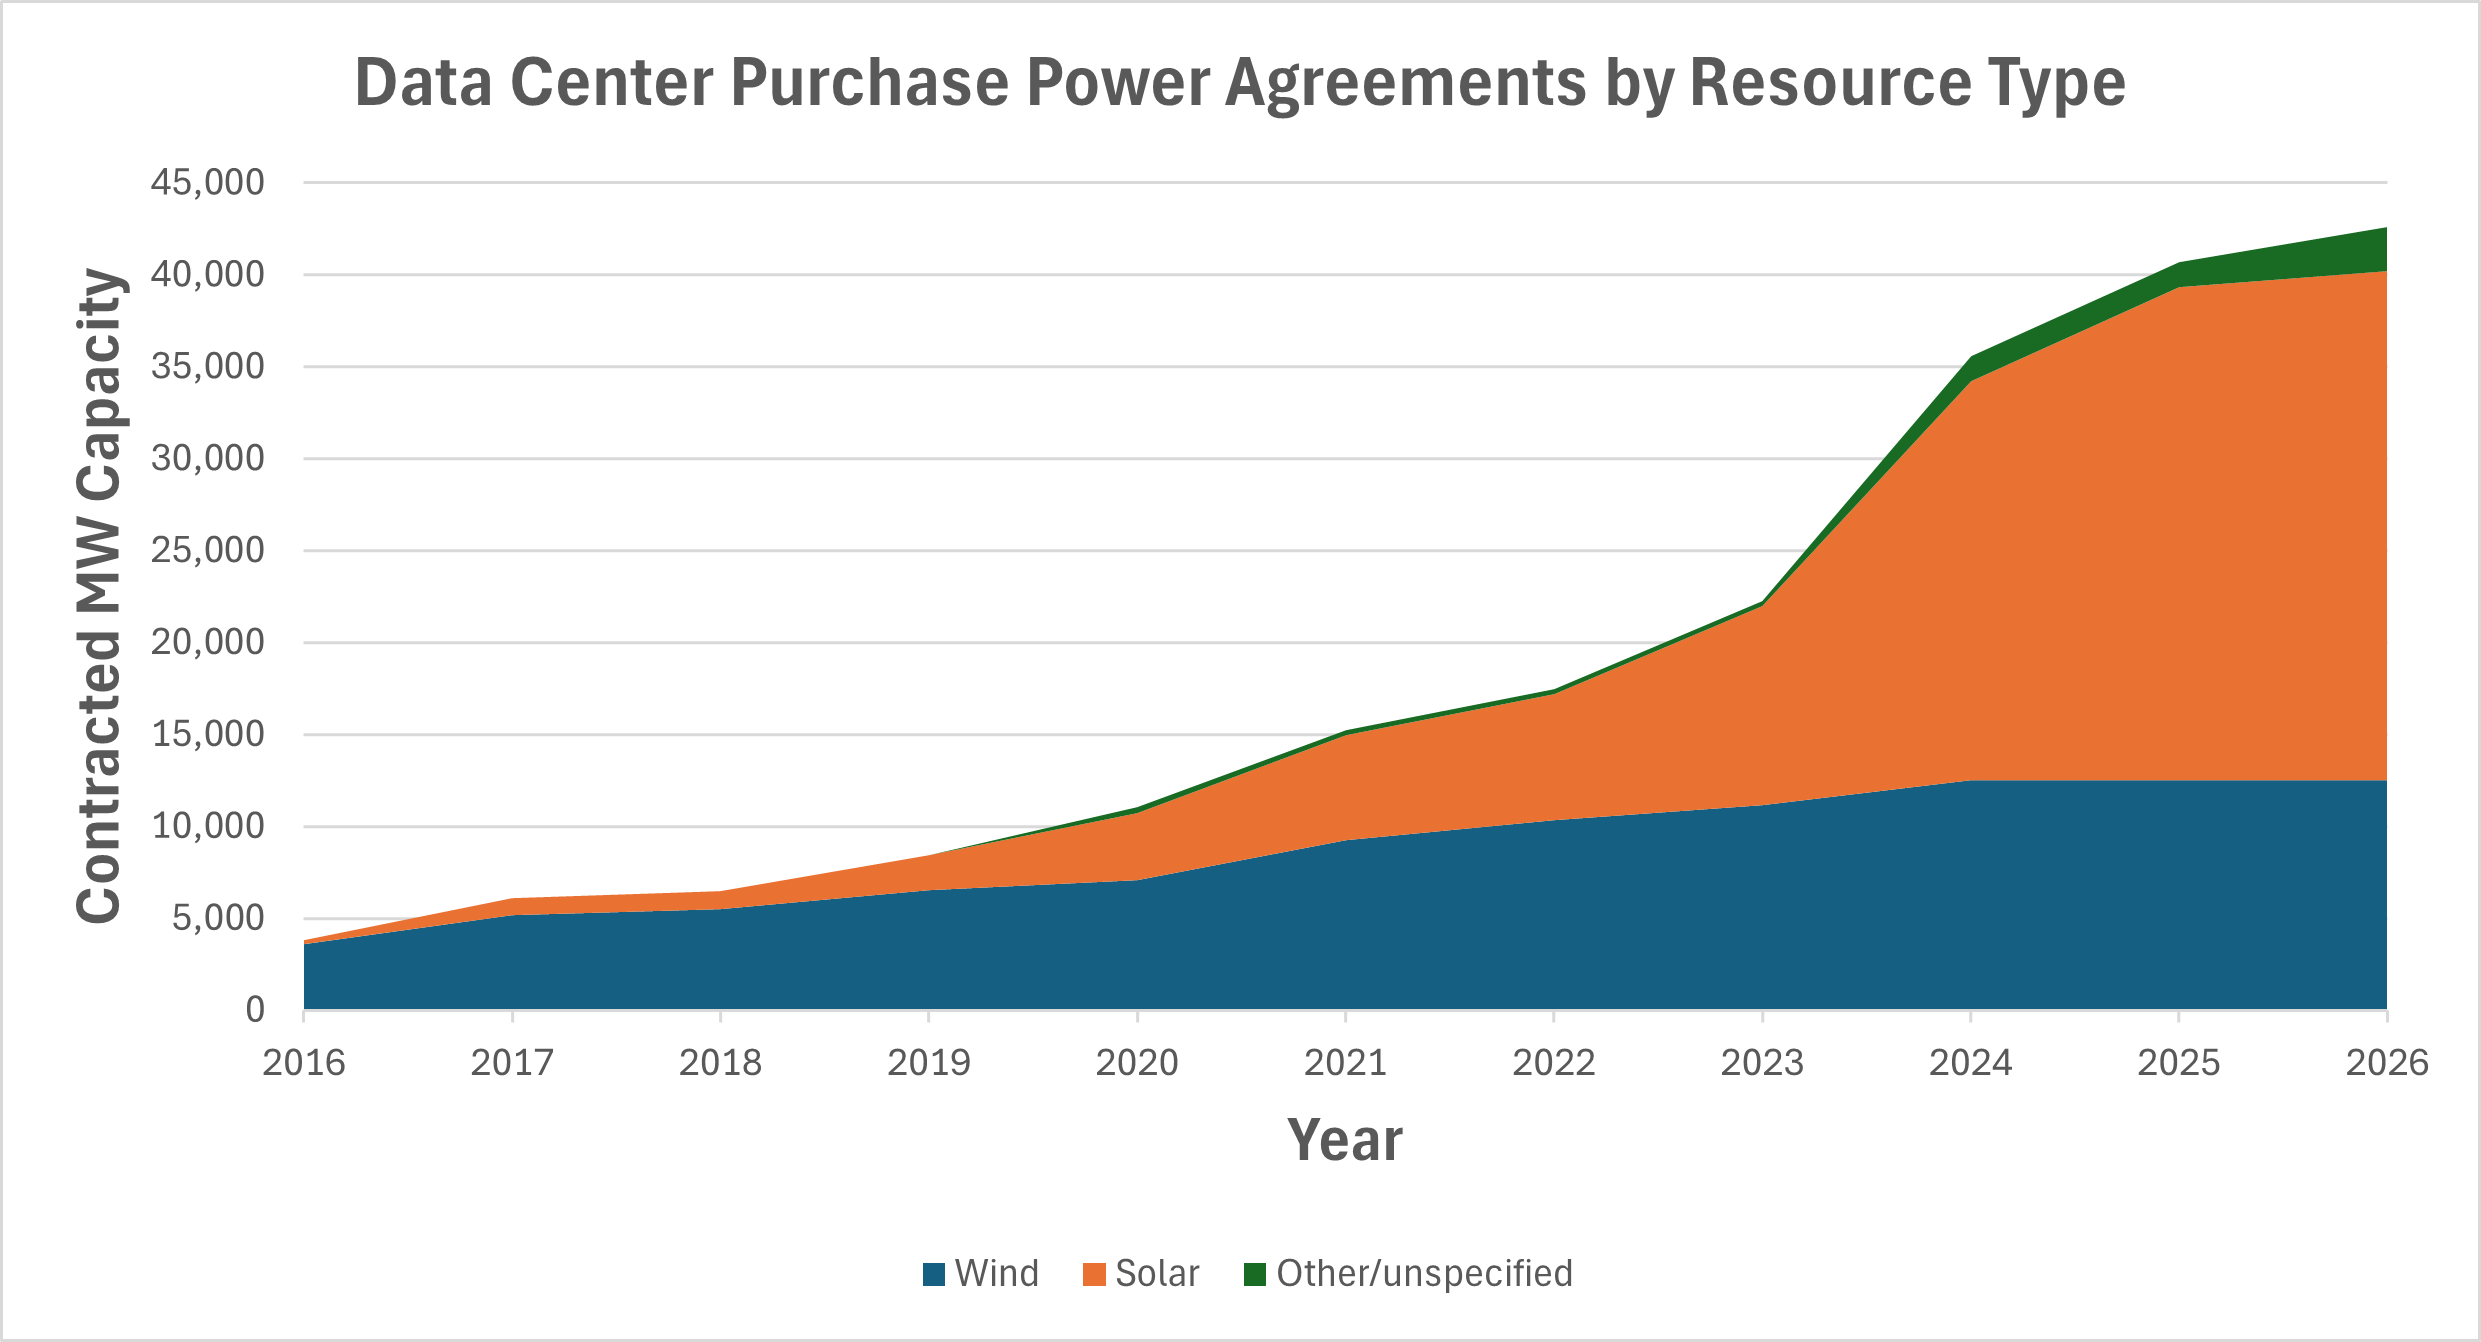
\includegraphics[width=0.75\linewidth]{Figures/PPA by Resource Type.png}
%     \caption{Data Center PPAs by Resource Type}
%     \label{fig:PPAbyResource}
% \end{figure}

% \begin{figure}
%     \centering
%     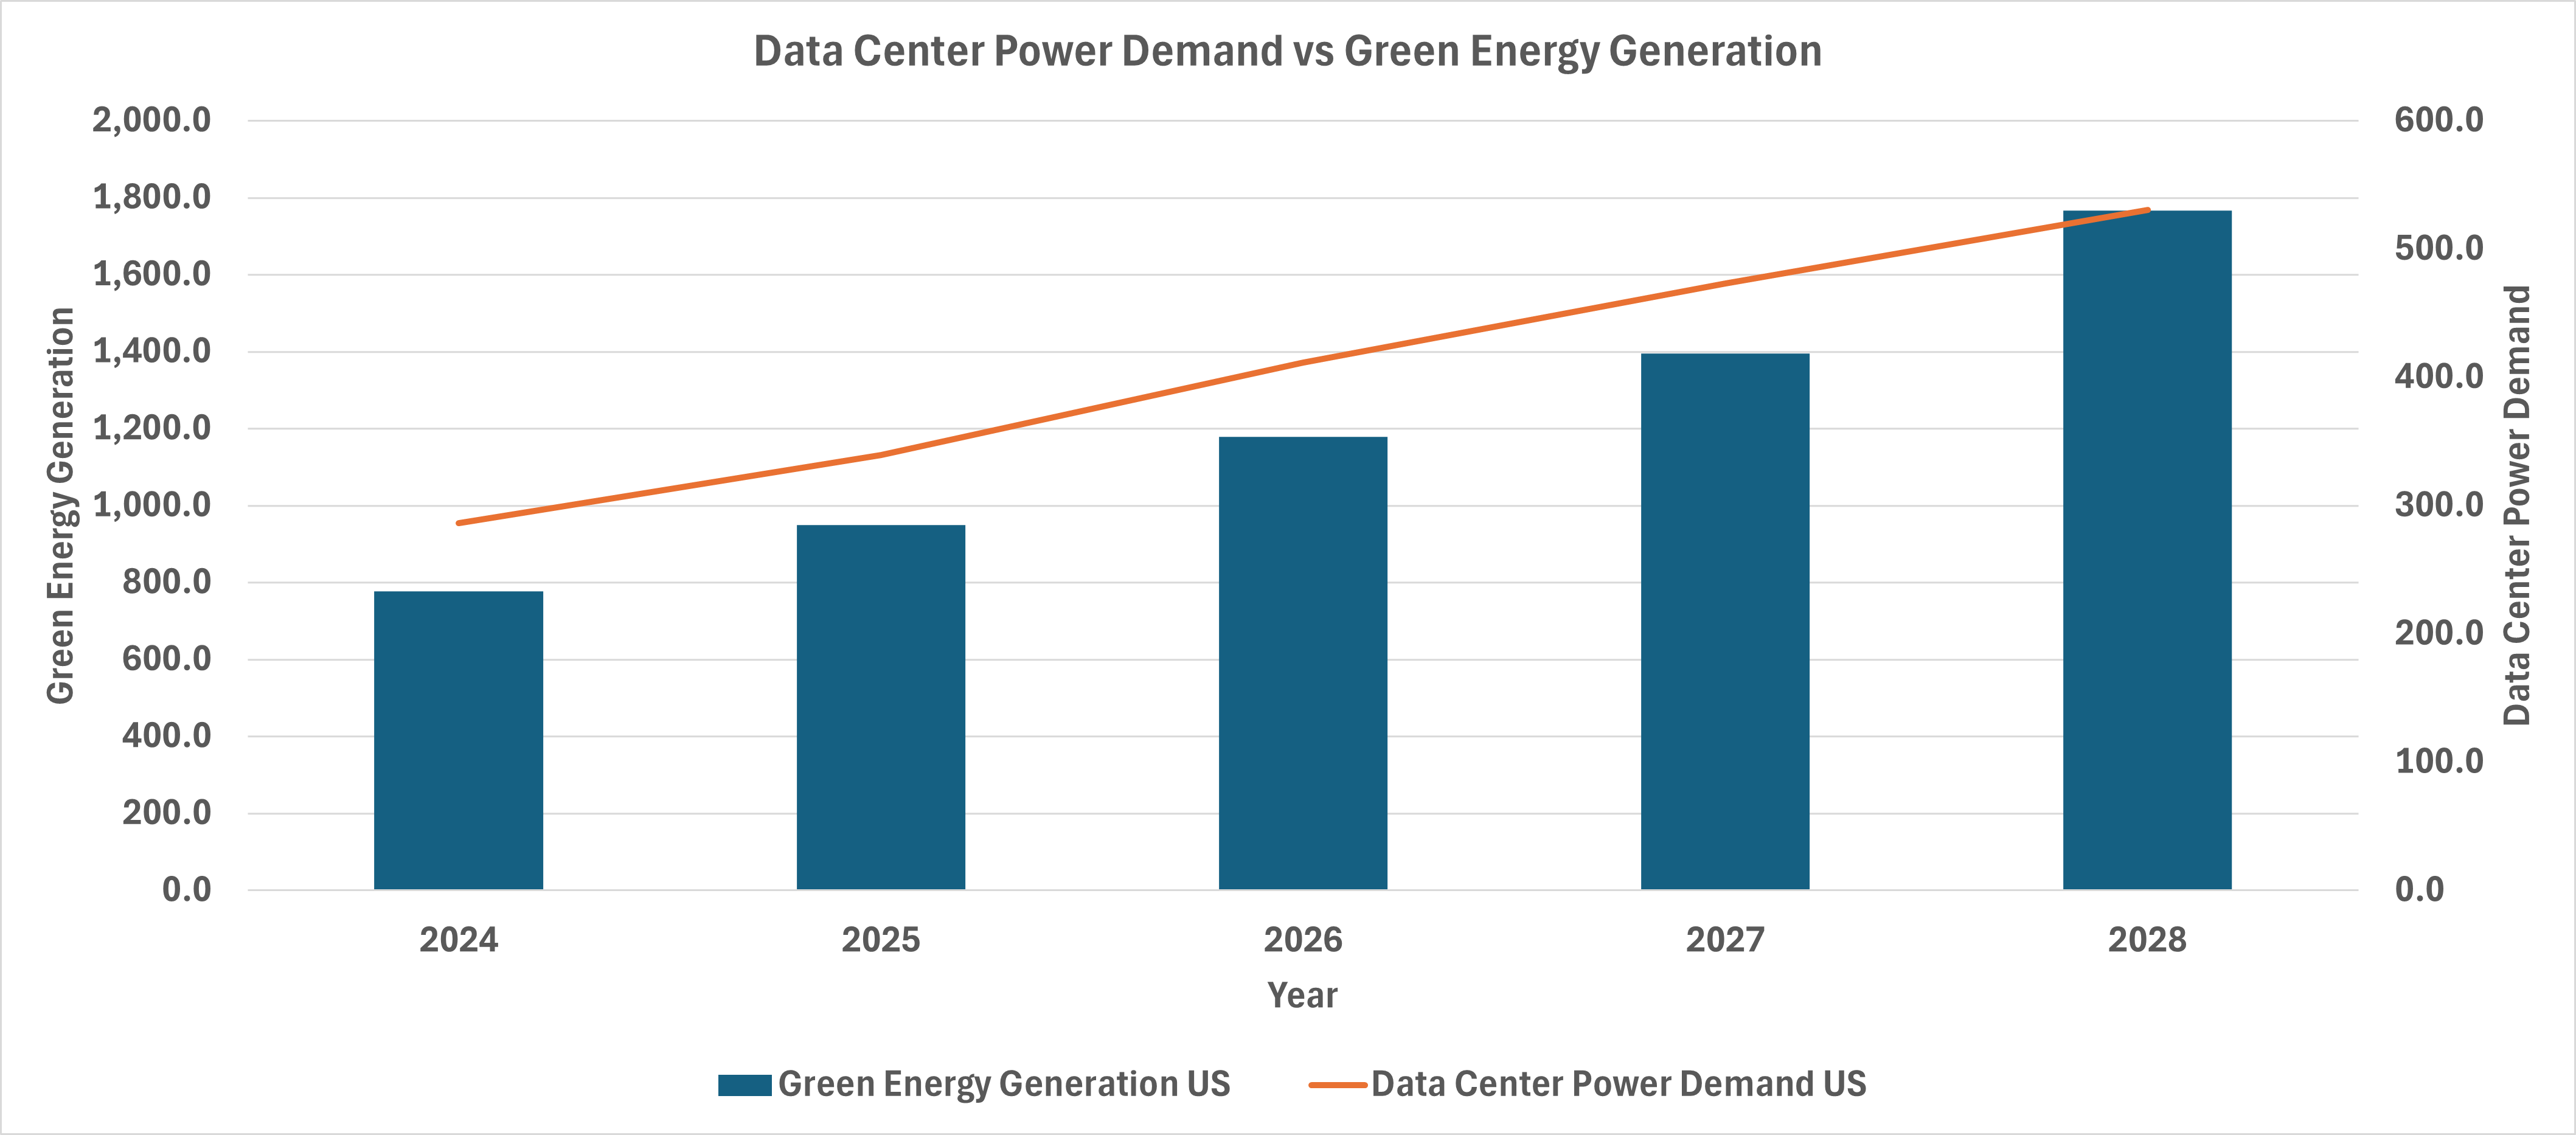
\includegraphics[width=0.5\linewidth]{Figures/Data Center Power Demand vs Green Generation.png}
%     \caption{Data Center Power Consumption vs Green Generation. Source: Aterio.io}
%     \label{fig:DCPowerConsumption}


\section{Results}\label{Sec::Results}
Our stacked DiD estimator (\autoref{subsec:eventstudy}) addresses potential bias from treatment effect heterogeneity in settings with staggered AI model releases. For all power quality and fossil demand effects, following \citet{callaway2021difference}, we construct cohort-specific datasets for each of the treatment events corresponding to major AI model publications through 2023, then stack these datasets to estimate a set of treatment effects across all dimensions. Table \ref{tab:combined_results} provides a full set of results from our main regressions including analysis of the impacts of on-site colocated generation for our counterfactuals.
%\nb{wouldnt know what these are at this point. Are these the $\beta_k$s?}. We compute price effects based on fossil demand effects.
% We estimate the effect of AI model deployment on electricity demand and power quality using a stacked difference-in-differences framework that addresses two identification challenges: (1) heterogeneous treatment timing across AI model releases, and (2) potential confounding from supply-side shocks that simultaneously affect electricity prices and quantities. Our primary specifications employ stacked event-study estimation, which allows us to trace out dynamic treatment effects and assess pre-trends. For power quality outcomes, where sample size constraints limit event-study precision, we supplement with two-way fixed effects (strict DiD) specifications that pool pre- and post-treatment periods into binary indicators. We then present robustness checks using alternative treatment definitions, followed by counterfactual exercises that explore how alternative evolutionary paths for AI compute might affect grid outcomes.


\subsection{Power Quality Effects: Utility-Level Strict DiD}

%We complement the generator-level demand analysis with an examination of power quality impacts at the utility service territory level. This analysis differs from the stacked event-study specification in several respects necessitated by data structure and sample size constraints.

%First, the unit of analysis shifts from individual generators to retail electric utility service territories (N = 71 utilities). Second, the outcome variables are the Consumer Power Quality Index (CPQI) and Total Harmonic Distortion (THD) rather than electricity demand. Third, treatment is defined as the presence of any AI-affiliated data center within the utility territory, rather than proximity to a specific facility. Fourth, the smaller sample size (1,136 utility-month observations) limits the precision of event-study coefficients, leading us to employ a strict two-way fixed effects (DiD) specification that pools pre- and post-treatment periods into binary indicators rather than tracing out event-time dynamics. We do not employ instrumental variables in this specification; the estimates capture the reduced-form relationship between AI data center presence and power quality outcomes.

%\subsubsection{Main Results}
We report the power quality effects of AI data centers in seventy one retail electric utility service territories estimated from power quality observations over 1136 utility-months. We use Consumer Power Quality Index (CPQI) and Total Harmonic Distortion (THD) as outcome variables in our stacked DiD models (~\autoref{eq:pq_eventstudy}). 

Table~\ref{tab:combined_results} reports results from the utility-level strict DiD specification. The CPQI coefficient speaks to the reliability of the power supply to the consumers. The CPQI coefficient of 0.3795 indicates a deterioration level that corresponds to moving from a typical U.S. power area toward the bottom quartile of power quality—roughly \textbf{the difference between $\sim$ 1 outage/year and $\sim$ 1.5–2 outages/year for the average customer}.Other reliability events such as brownouts and surges are predicted to increase by ~1-2 per year. Importantly, power surges are a known ignition source for electrical fires, contributing to the approximately 51,000 annual residential electrical fires in the U.S., with electrical arcing accounting for 74\% of ignition sources \cite{usfa2019electrical}. Fewer fires is generally considered a desirable outcome amongst electricity professionals \cite{Laughner2024THD}.
%\nb{Add brownouts or other reliability events}
\footnote{These are calculated based on Whisker Labs description of the CPQI Score with a description of derivation in the appendix.} This implies more frequent voltage anomalies that make motors and electronics run less efficiently and age faster.



The post-treatment coefficient of 0.0625 for THD indicates that utility territories containing AI data centers experienced a 0.0625 percentage point increase in readings above the 0.8 distortion threshold following AI model releases. 
%\nb{A 0.06\% increase reads negligible. Can we add something that makes the impact clearer, likely, and concrete. For example you could say: While a fraction of a percentage point might seem a negligible effect, in practice this level of increase can cause substantial problems. For example, this level of increase will halve the lifespan of ....} 
While a 0.0625 percentage point increase may appear small in isolation, the IEEE 519 standard exists precisely because even modest increases in harmonic distortion impose continuous thermal stress on motor windings. According to the Arrhenius equation underlying motor insulation ratings, every 10°C rise in operating temperature halves insulation life \cite{NEMA_MG1}. Since elevated THD causes motors to waste additional power as heat in their iron and copper windings \cite{Laughner2024THD}, sustained exposure compounds over the multi-year lifespans of household appliances, accelerating degradation of refrigerators, air conditioners, and other motor-driven equipment.

%(\nb{e.g. reducing the lifespan of a microwave by X}).

%indicates that the surrounding area can expect an additional reliability event per year. This level of deterioration in CPQI corresponds to moving from a typical U.S. area toward the bottom quartile of power quality—roughly \textbf{the difference between $\sim$ 1 outage/year and $\sim$ 1.5–2 outages/year for the average customer}\footnote{These are calculated based on Whisker Labs description of the CPQI Score with a description of derivation in the appendix.}—and implies more frequent voltage anomalies that make motors and electronics run less efficiently and age faster. \nb{Can we also add something about how much faster a specific appliance (say a microwave) could age under this level of power quality deterioration?}


% \begin{table}[h]
% \centering
% \caption{Utility-Level Power Quality Results: Two-Way Fixed Effects (Strict DiD) along with the quality of fit metric ($R^2$).  \nb{Get rid of N and SE}}
% \label{tab:thd_results}
% \begin{tabular}{lcccc}
% \toprule
% Outcome & Post Coefficient & SE & $R^2$ & N \\
% \midrule
% THD ($>$0.8 threshold) & 0.0625*** & $<$0.001 & 0.956 & 1,136 \\
% CPQI & 0.3795*** & $<$0.001 & 0.956 & 1,136 \\
% \bottomrule
% \end{tabular}
% \begin{flushleft}
% \footnotesize\textit{Notes:} *** p < 0.001. Utility and time fixed effects with cluster-robust standard errors. Treatment defined as presence of AI-affiliated data center in utility service territory.
% \end{flushleft}
% \end{table}

\subsection{Fossil Fuel Demand Effects: Stacked DiD Estimation}

We estimate Fossil Fuel Demand effects using demand data from a total of 35.6 million generator-hour observations, which includes 900,956 treated observations from generators located within 20 miles of AI-affiliated data centers and the other 34.7 million from other generators as control observations.

%\nb{move this to the robustness results and change table 3. Expand, at least once, OLS and 2SLS. Better yet unify terminology.}
We estimate the baseline specification via two-stage least squares (2SLS) to isolate demand-side effects from supply shocks. All specifications include zone and month fixed effects with standard errors clustered by unit-event. Further details on the instrumental variables specification can be found in Appendix Subsection \ref{IVDetails}. Table~\ref{tab:combined_results} reports the full stacked DiD coefficients.

% \nb{Change to new terminology. No event-study anymore.}
\paragraph{Stacked DiD Coefficients: OLS versus 2SLS.} Table~\ref{tab:combined_results} reports the full stacked DiD coefficients from both specifications. Figure \ref{fig:event_study_main} shows the stacked DiD coefficients for power demand in the 2SLS specification. The $t=+2$ coefficient shows a significant demand increase of 5.20 MWh, representing the demand shift at generators near data centers two months after AI model release, isolated from supply-side price variation through our instrumentation strategy. The pre-treatment coefficient at $t=-2$ is highly significant, representing demand created by training. While these effects may not seem large enough to be economically interesting, these effects are hourly and by generator. When the aggregate impact is calculated, they represent over 500 additional GWh added nearby to a data center over the inference period in some cases. \textbf{The additional power is roughly equivalent to that of 47,000 household-years in the United States}.

% \begin{table}[h]
% \centering
% \caption{Stacked DiD Coefficients: Generator-Level Demand}
% \label{tab:event_study}
% \begin{tabular}{lccccc}
% \toprule
% & \multicolumn{2}{c}{OLS} & & \multicolumn{2}{c}{IV 2SLS} \\
% \cmidrule{2-3} \cmidrule{5-6}
% Event Time & Coefficient & SE & & Coefficient & SE \\
% \midrule
% $t = -2$ & +1.28 & (1.29) & & +6.33*** & (1.63) \\
% $t = -1$ & \multicolumn{2}{c}{[reference]} & & \multicolumn{2}{c}{[reference]} \\
% $t = 0$ & $-4.39$ & (3.10) & & +0.69 & (2.79) \\
% $t = +1$ & $-1.64$ & (2.80) & & +0.74 & (2.45) \\
% $t = +2$ & +1.31 & (2.27) & & +5.20** & (2.54) \\
% \midrule
% Pre-treatment avg & \multicolumn{2}{c}{+1.28} & & \multicolumn{2}{c}{+6.33} \\
% Post-treatment avg & \multicolumn{2}{c}{$-1.57$} & & \multicolumn{2}{c}{+2.21} \\
% \bottomrule
% \end{tabular}
% \begin{flushleft}
% \footnotesize\textit{Notes:} *** p < 0.01, ** p < 0.05. N = 35.6 million observations from 19 treatment events. Standard errors clustered by unit-event. IV instruments: natural gas price $\times$ zone-average heat rate.
% \end{flushleft}
% \end{table}

% The OLS specification shows no significant effects in any period, consistent with the parallel trends validation. Figure \ref{fig:event_study_main} shows the stacked DiD coefficients for power demand in the 2SLS specification. The 2SLS specification reveals two notable patterns. First, the $t=-2$ coefficient is significant (6.33, p < 0.01) indicating a significant traning demand increase.. Second, the $t=+2$ coefficient shows a significant demand increase of 5.20 MWh (SE = 2.54, p < 0.05), representing the demand shift at generators near data centers two months after AI model release, isolated from supply-side price variation through our instrumentation strategy. While these effects may not seem large enough to be economically interesting, these effects are hourly and by generator. When the aggregate impact is calculated, they represent over 500 additional GWh added nearby to a data center over the inference period in some cases. \textbf{The additional power is roughly equivalent to that of 47,000 household-years in the United States}. This further strains grids as the power is not evenly distributed across hours. The pre-treatment coefficient at $t=-2$ is significant, representing demand created by training, but prior to treatment, the trends are identical with the control sample. Figure~\ref{fig:event_study_main} displays stacked DiD coefficients for the pre-treatment and post-treatment windows from the OLS specification. 
\begin{figure}[th!]
    \centering
    % Note: Reference the actual output files from stacked_did_iv_results/
    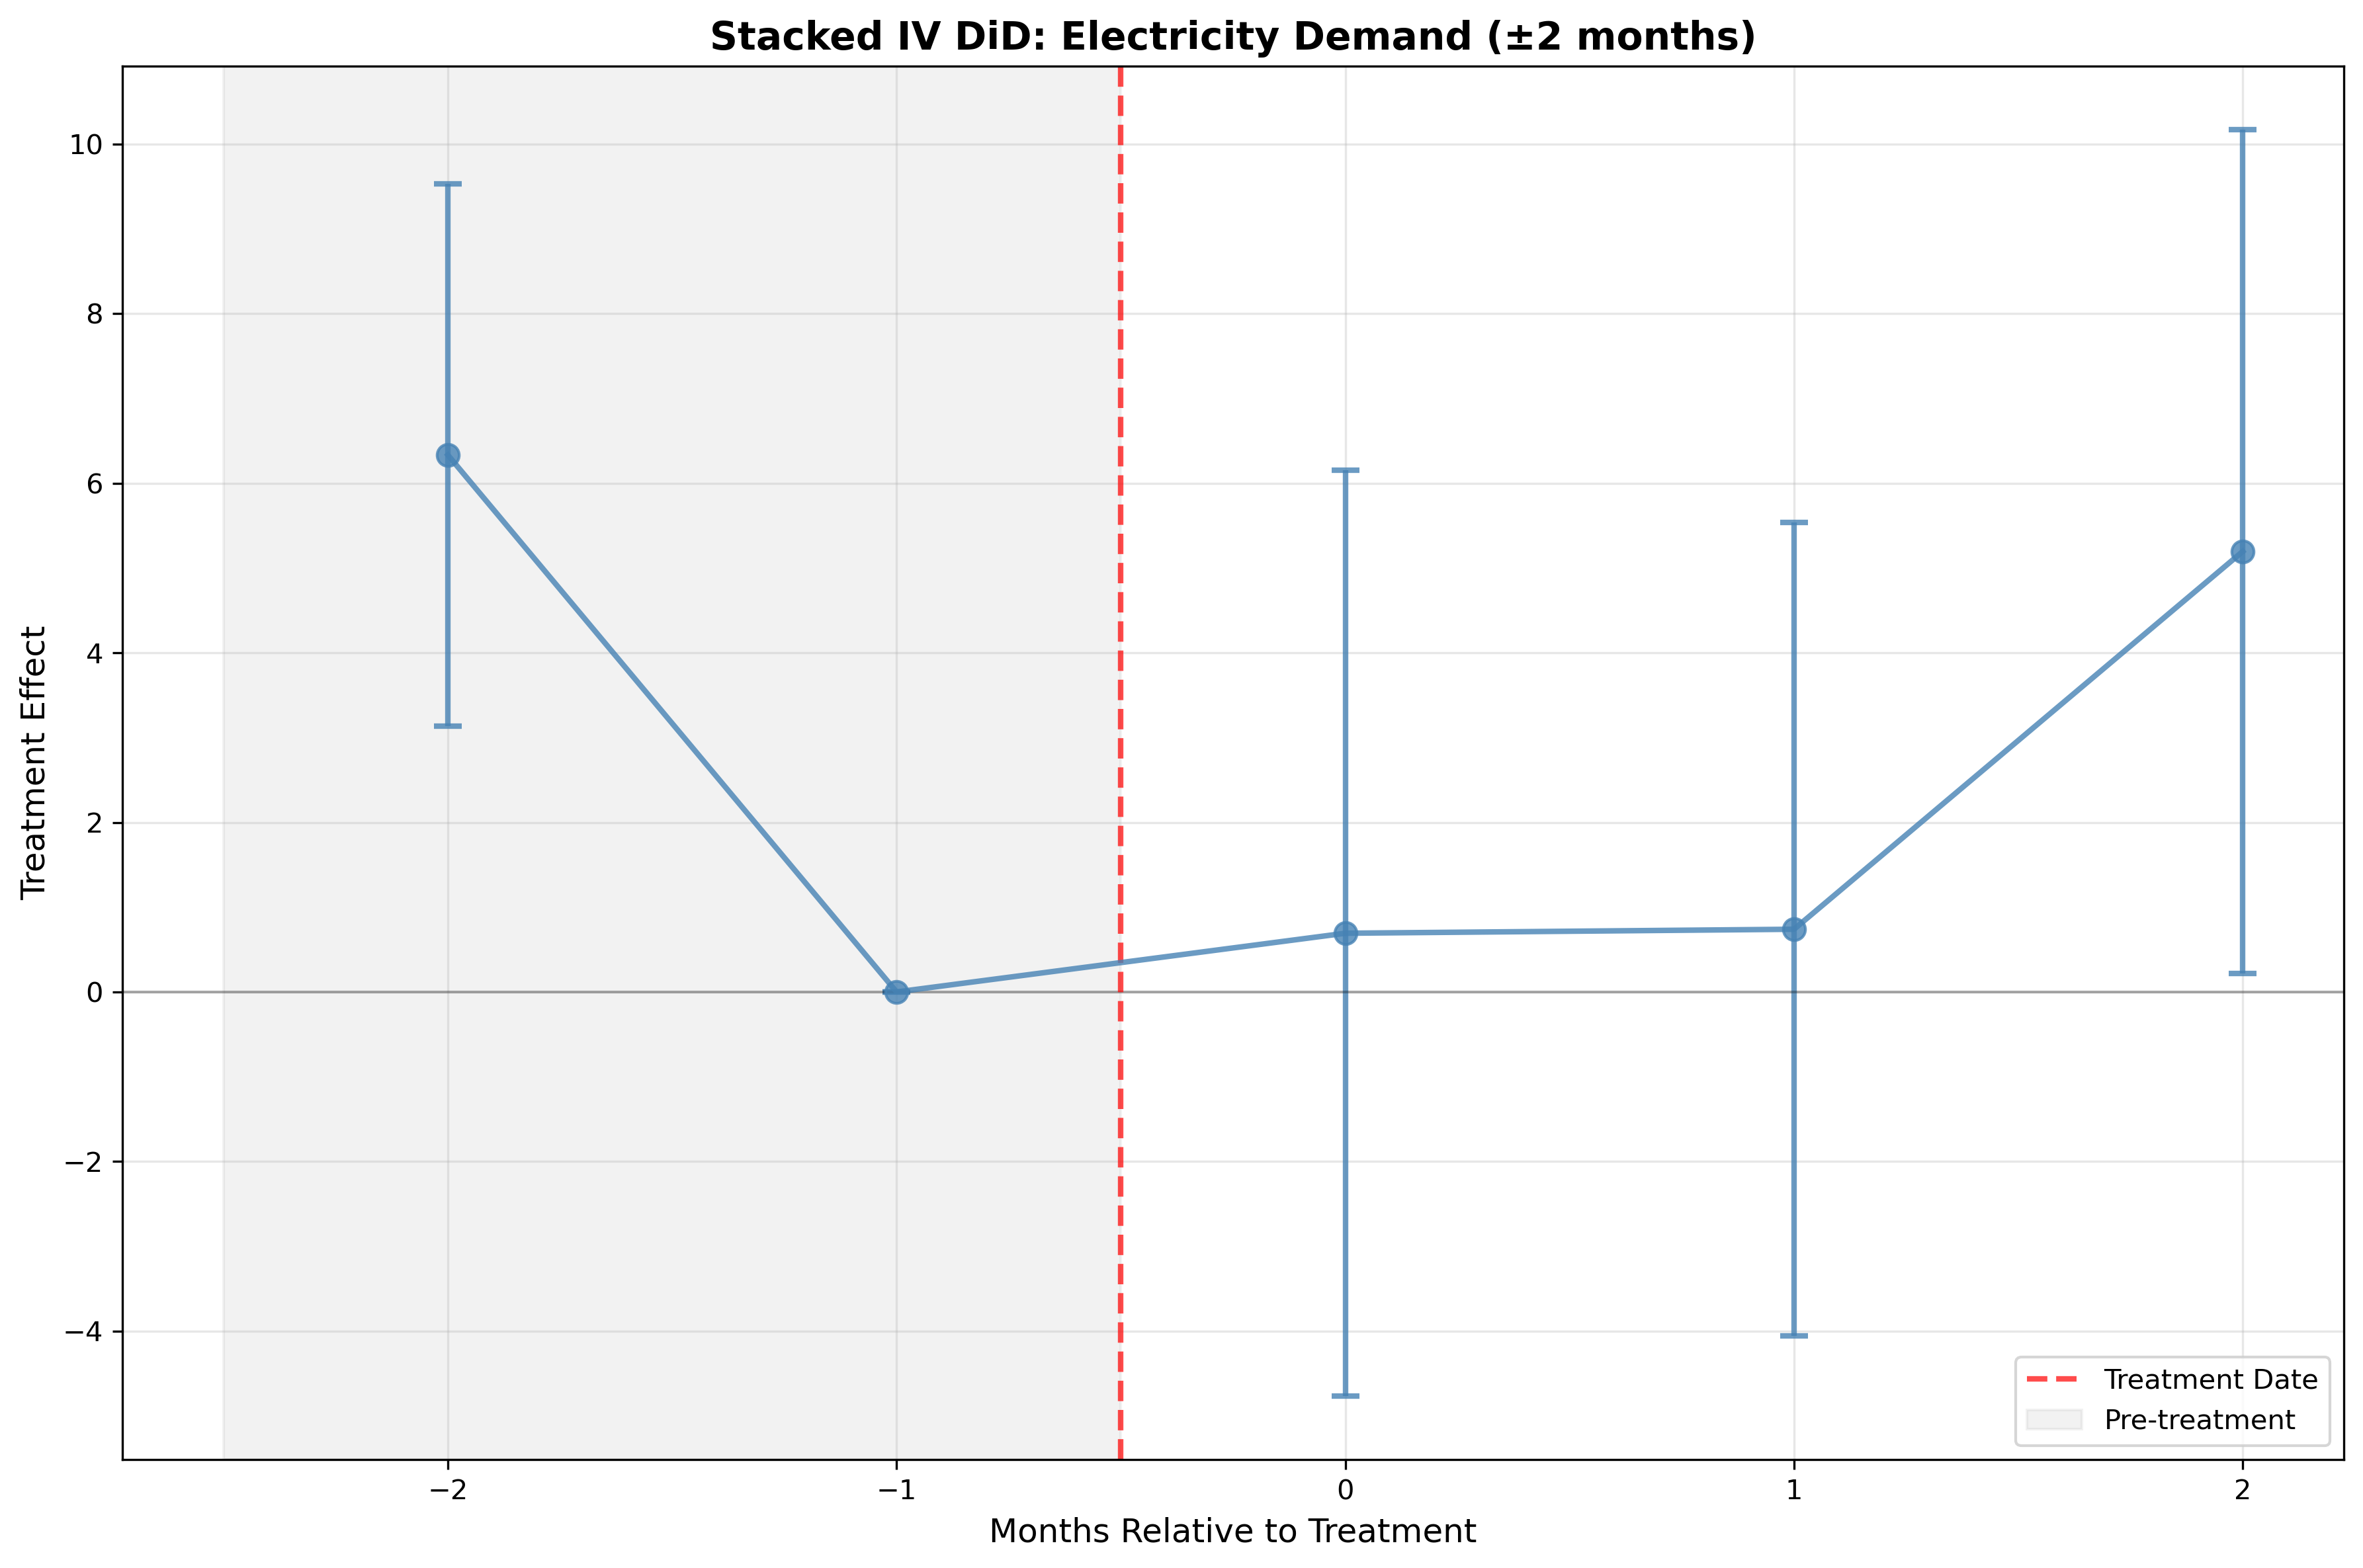
\includegraphics[width=0.8\linewidth]{Figures/event_study_iv.png}
    \caption{Stacked DiD coefficients for power demand (IV specification). Event Time 0 corresponds to AI model publication date. The pre-treatment coefficient at $t=-2$ demonstrates the training demand. Reference period is $t=-1$.}
    \label{fig:event_study_main}
\end{figure}

\begin{table*}[t]
\centering
\caption{Summary of Estimation Results Across Specifications}
\label{tab:combined_results}
\begin{tabular}{llcp{7.5cm}}
\toprule
Analysis & Outcome & Coefficient & Effect Interpretation \\
\midrule
\multicolumn{4}{l}{\textit{Panel A: Utility-Level Power Quality (Two-Way FE)}} \\
\addlinespace[0.5em]
Strict DiD & THD ($>$0.8) & 0.0625*** & More outages and equipment failure. \\
Strict DiD & CPQI & 0.3795*** & Moving from typical U.S. power quality to the bottom quartile; increases annual outages for the average customer from approximately 1 to 1.5–2. \\
\addlinespace[0.5em]
\midrule
\multicolumn{4}{l}{\textit{Panel B: Generator-Level Demand (Stacked DiD)}} \\
\addlinespace[0.5em]
OLS & Pre-treatment avg & +1.28 & \multirow{4}{7.5cm}{Aggregate impact represents over 500 additional GWh near data centers over the inference period—equivalent to $\sim$47,000 U.S. household-years of consumption, with load not evenly distributed across hours} \\
OLS & Post-treatment avg & $-1.57$ & \\
IV 2SLS & Pre-treatment avg & +6.33*** & \\
IV 2SLS & Post-treatment avg & +2.21 & \\
\addlinespace[0.5em]
\midrule
\multicolumn{4}{l}{\textit{Panel C: Power Quality by On-Site Generation Status}} \\
\addlinespace[0.5em]
With on-site & CPQI & $-0.122$*** & \multirow{3}{7.5cm}{On-site Generation generation mitigates grid stress from AI load; utilities without on-site experience reliability deterioration while those with on-site see improvements} \\
Without on-site & CPQI & +0.228*** & \\
Difference & CPQI & $-0.350$*** & \\
\bottomrule
\end{tabular}
\begin{flushleft}
\footnotesize\textit{Notes:} *** $p < 0.001$, ** $p < 0.05$. Panel A: Utility and time fixed effects with cluster-robust standard errors; treatment defined as presence of AI-affiliated data center in utility service territory. Panel B: 35.6 million observations from 19 treatment events; standard errors clustered by unit-event; IV instruments: natural gas price $\times$ zone-average heat rate. Panel C: CPQI = Consumer Power Quality Index; THD = Total Harmonic Distortion.
\end{flushleft}
\end{table*}


% \subsubsection{Parallel Trends Validation}

% We first assess the parallel trends assumption underlying our identification strategy.


\subsection{Price Impacts}

% We estimate wholesale electricity price impacts by combining our demand estimates with supply curve parameters, following the methodology outlined in Section \ref{PriceEffects}. This approach recognizes that our IV strategy identifies demand shifts but does not directly estimate equilibrium price effects\nb{expand this terminology as a footnote}. The price impact of AI-induced demand depends on the slope of the supply curve\nb{footnote explaining what this is}: inelastic supply\nb{expand this terminology} implies large price effects, while elastic supply implies small effects. Additional specifics on calculation methodology can be found in Appendix Subsection \ref{CalcMethodologyPrice}. 

We estimate wholesale electricity price impacts by combining our demand estimates with supply curve parameters, following the methodology outlined in Section \ref{PriceEffects}. This approach recognizes that our IV strategy identifies demand shifts but does not directly estimate equilibrium price effects.\footnote{Our instrumental variables approach isolates exogenous variation in electricity demand driven by AI model releases. However, observed market prices reflect the intersection of supply and demand in equilibrium. To translate our demand estimates into price effects, we must incorporate information about supply-side responses, which requires additional assumptions about the shape of the supply curve.} The price impact of AI-induced demand depends on the slope of the supply curve\footnote{The supply curve describes the relationship between price and quantity supplied. Its slope reflects how much generators must be compensated to produce additional electricity—steeper slopes indicate that marginal generation costs rise quickly as output expands, typically because higher-cost units must be dispatched.}: inelastic supply—where quantity supplied responds weakly to price changes—implies large price effects, while elastic supply implies small effects. Additional specifics on calculation methodology can be found in Appendix Subsection \ref{CalcMethodologyPrice}.

A map of estimated supply chain elasticities can be found in Figure \ref{PJMPRiceElasticity} in Appendix section \ref{PriceElasticityAppendix} demonstrates the supply elasticity by zone in PJM. Figure \ref{PJMPrice} showing price increase estimates by zone. On average AI training leads to \textbf{substantial increases in wholesale prices in PJM with the highest increase surpassing 25\% in the American Electric Power (AEP) Zone}. Additional caveats are provided in Appendix Subsection \ref{appendix:Caveats}

\begin{figure}
    \centering
    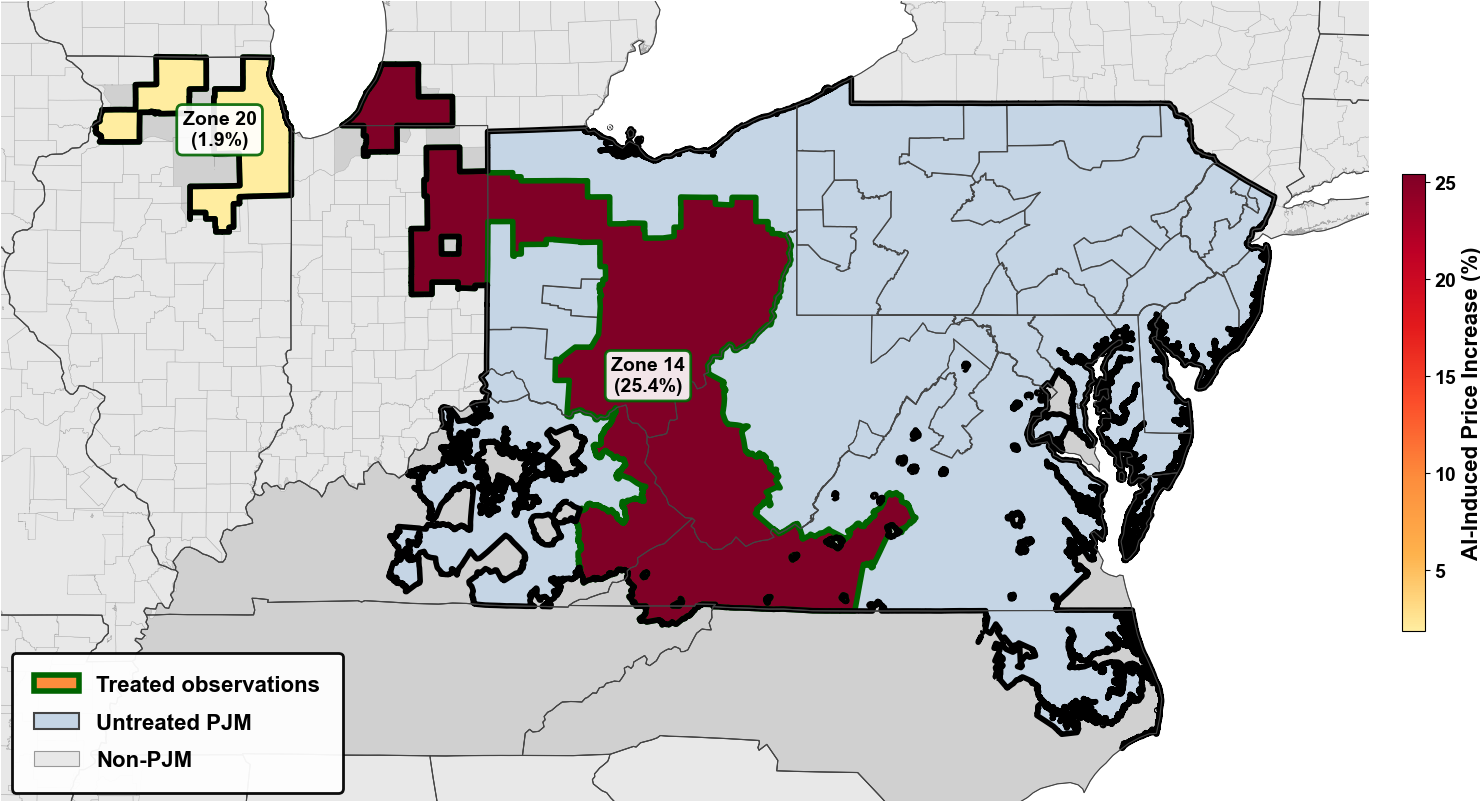
\includegraphics[width=0.75\linewidth]{Figures/PJMMap3.png}
    \caption{Price Effects of AI in PJM.}
    \label{PJMPrice}
\end{figure}

While we are not able to provide definite evidence of the impacts on retail price pass through, it should be noted that retail electricity prices have increased overall at a rate surpassing inflation since 2020 \cite{Nicoletti_Malik_Tartar_2024,horsley2025electricbill,spp2024stateofthemarket}. While it is possible that increased investment in electric generation through power purchase agreements by tech firms may in the long run lead to falling retail prices, it appears that at present data center power usage is increasing wholesale prices by raising total demand, which requires dispatching higher-cost generators and thus increases the market clearing price—a price paid by all retail consumers.

Using estimates from the literature as documented in Appendix Subsection \ref{WholesaleRetailPassthrough}, we can bracket the expected price rise for retail consumers. Two recent estimates apply but speak to different horizons. \cite{defeuilley2023pennsylvania} report short-run passthrough of roughly $0.53$--$0.56$ in PJM/Pennsylvania over a sample window dominated by short retail-rate refresh cycles and explicit fuel-cost-adjustment provisions; applying that passthrough to a 25\% wholesale shock in AEP implies a short-run consumer price rise of roughly 13\%. \cite{mackay2024wholesale} estimate long-run passthrough closer to one across U.S.\ retail markets, on the assumption that procurement contracts, default-service auctions, and rate-case filings eventually fully reflect sustained wholesale movements; under that estimate the long-run consumer price rise approaches the full 25\%. The two numbers therefore correspond to short-run vs.\ long-run passthrough rather than to competing estimates of the same object: the 13\% figure is the appropriate near-term magnitude for retail bills under existing PJM rate mechanics, while the 25\% figure is the appropriate long-run magnitude if the wholesale shock is sustained for several rate cycles. We report both and let the reader weight them according to the policy horizon of interest, rather than collapsing to a single point estimate.
\section{Validating Assumptions and Robustness Checks}\label{Robustness}
% \nb{refer to earlier mention of issues}
We conduct several additional analyses to probe the robustness of our findings and explore effect heterogeneity in order to address issues highlighted in Subsection \ref{DCASSUmptions}. The formal testing helps provide evidence for the parallel trends assumption while the placebo tests address potential issues related to external confounds or lack of specific knowledge about training. Additional robustness analyses can be found in Appendix Subsection \ref{App:AdditionalRobustnessChecks}.

\subsubsection{Formal Testing for Parallel Trends}

 For power demand specifically, the formal joint test of pre-treatment coefficients yields a chi-squared statistic of 0.99 (df = 1) with p-value = 0.3196. \textbf{We cannot reject the null hypothesis of parallel pre-trends at conventional significance levels.} This provides support for our identification assumption: treated and control generators followed similar demand trajectories prior to AI model releases. Some of our samples demonstrate significant evidence against the the parallel trends test prior to propensity score matching. However, in 100\% of our samples for both power quality and power demand after propensity score matching, we \textit{fail to reject the null hypothesis of }. This implies that the technique correctly handles the issue where it exists. 
 
 Additionally, We estimate the baseline specification via OLS to validate parallel trends prior to implementing our instrumental variables strategy. The OLS specification shows no significant effects in any period outside the training window, consistent with parallel trends holding in the pre-treatment period. Importantly, prior to treatment (excluding $t=-2$, which captures training demand), the trends are identical between treatment and control samples. Figure~\ref{fig:event_study_main} displays stacked DiD coefficients for both pre-treatment and post-treatment windows, with the reference period at $t=-1$.

 \subsubsection{Placebo Tests}
We conduct three placebo exercises to assess the validity of our identification strategy. First, to distinguish AI-specific effects from general data center growth, we estimate treatment effects using our 12,283 non-AI data centers as a placebo treatment group. If estimated effects simply reflect data center proximity rather than AI workloads specifically, we would expect similar magnitudes in this specification. The non-AI CPQI coefficient (0.228, p < 0.001) matches the AI data center coefficient for facilities without on-site generation, suggesting that general data center load---not AI workloads specifically---drives some of the observed power quality effects. However, the demand-side 2SLS estimates from the stacked DiD, which leverage AI model release timing, remain distinct from this general data center effect.

Second, we implement random date and random location placebo tests. Both yield a p-value of 1.00 for the coefficient in our fossil fuel demand, CPQI, and THD analyses, confirming that our results do not arise from spuriously chosen locations or dates.

% \subsubsection{Non-AI Data Center Placebo}

% To distinguish AI-specific effects from general data center growth, we estimate treatment effects using our 12,283 non-AI data centers as a placebo treatment group. If estimated effects simply reflect data center proximity rather than AI workloads specifically, we would expect similar magnitudes in this specification.

% The non-AI CPQI coefficient (0.228, p < 0.001) matches the AI data center coefficient for facilities without BTM generation, suggesting that general data center load---not AI workloads specifically---drives some of the observed power quality effects. However, the demand-side 2SLS estimates from the stacked event-study, which leverage AI model release timing, remain distinct from this general data center effect.

% \subsubsection{Random Dates and Random Locations Placebos}

% Both random dates and random locations yield a p-value of 1.00 for the coefficient in our fossil fuel demand, CPQI, and THD analyses. This suggests that our results are not the result of randomly chosen locations or dates.

\section{Counterfactual Analyses}
\label{sec:counterfactuals}

We present three main counterfactual exercises to inform stakeholders and policymakers about how alternative evolutionary paths for AI compute might affect grid outcomes. These combine our econometric estimates with data on model characteristics and infrastructure configurations to explore three dimensions: model scaling, geographic redistribution, and workload composition. Our counterfactual policies highly align with the implications of our theoretic model, particularly when considering the role of on-site generation as a solution to the challenges facing power procurement.\\

\noindent\textbf{1) Model Scaling.} We combine data on model size (parameter counts) with our econometric estimates from our least conservative specification to extrapolate grid impacts at different scales.

\noindent\textbf{(a) Power Quality.} Fitting a trend line to power quality impacts for Llama-3.1 (405B), PaLM (540B), and Llama 4 Behemoth (2T), we find that scaling from a 2 trillion parameter model to a 4 trillion parameter model would increase power quality impact from \textbf{0.321 to 0.434}---a deterioration of roughly 0.113 units, or just over 35\% relative to the 2 trillion baseline. The relationship is exponential over log parameter counts, implying that larger models require proportionally greater parameter reductions to achieve the same percentage improvement in power quality. \textbf{(b) Power Demand.} Using an analogous extrapolation, we find that \textbf{each 1\% parameter increase leads to approximately 0.15\% higher power demand} within three months of model release. Scaling from 540 billion to one trillion parameters would \textbf{increase total power demand by 10.5\%}. For DALL-E, halving parameters would \textbf{reduce inference demand by approximately 300 GWh}---equivalent to the annual consumption of 27,000--30,000 homes.\\

\noindent\textbf{2) Training Compute.} Training compute requirements also have measurable effects: a 1\% increase in training FLOPs is associated with a \textbf{0.1\% increase in power demand}. For GPT-3.5, halving training compute would reduce energy use by enough to power 8,000--10,000 U.S.\ homes for a year.\\

\noindent\textbf{3) Colocated On-site Generation.} Data centers increasingly deploy colocated on-site generation to reduce grid dependence. Our inventory identifies 87 facilities with on-site capability and 12,401 without. We test whether on-site capacity moderates estimated effects by interacting treatment with on-site status in the utility-level strict DiD specification. Results indicate that on-site generation substantially mitigates measured grid impacts. The sign reversal for CPQI is notable: data centers \textit{with} on-site generation are associated with improved power quality (negative coefficient), while those \textit{without} are associated with deterioration (positive coefficient). This heterogeneity suggests that \textbf{on-site generation absorbs demand spikes that would otherwise propagate to the grid}, and that aggregate grid impacts may understate total AI energy consumption.

Figure~\ref{fig:CounterfactualCombined} extends this to policy-relevant scenarios. Remarkably, universal adoption of on-site power would shift impact of data centers from a net detriment to power quality to a net improvement.\\
%However, all large AI data centers in our most conservative sample had on-site generation, which may exaggerate our estimates of colocated on-site generation's moderating effects.\nb{This statement again is a bit hard to parse. Does it undercut the impact statement above or support it?}

% \begin{figure}[h]
%     \centering
%     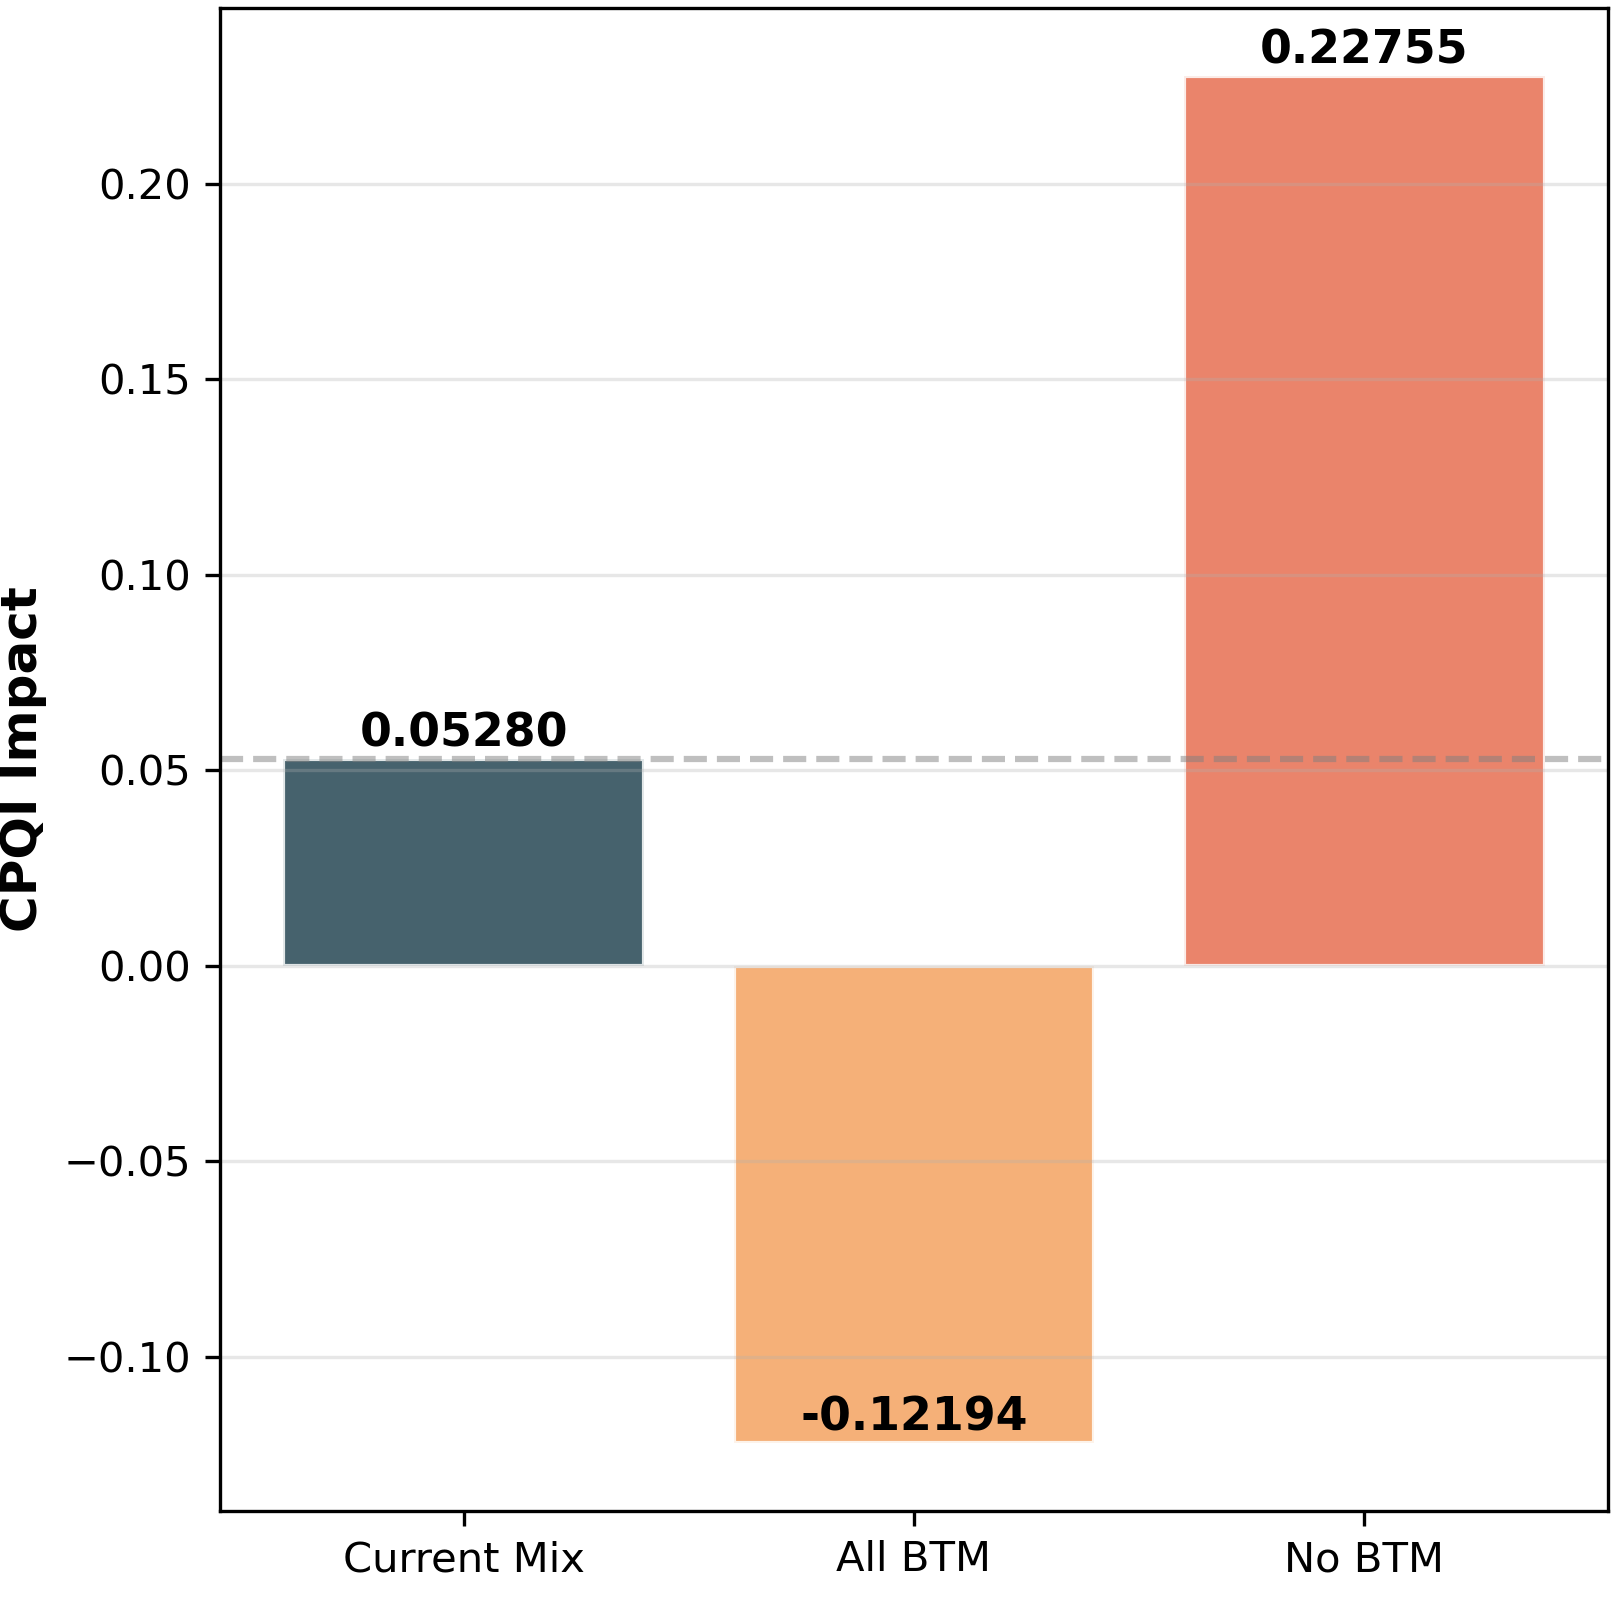
\includegraphics[width=0.35\linewidth]{Figures/btm_scenarios_analysis.png}
%     \caption{Impact of on-site power adoption on AI energy impacts.\nb{Dana it might be useful to collate plots in 5,6,and7 into a single figure laid side by side going across the two columns. this will save white space but also help make the figures bigger.}}
%     \label{fig:btm_scenarios}
% \end{figure}

\noindent\textbf{4) Geographic Redistribution}

%We analyze grid impacts under alternative spatial distributions of AI compute.

\noindent\textbf{(a) Distributed Inference (Edge Computing).} In our sample where we know AI data centers but not specific training and inference sites, we simulate a shift from cloud-based to edge-based inference, redistributing inference demand from concentrated hyperscaler facilities to smaller data centers located closer to population centers. Under this scenario, total demand added in a particular zone falls from a baseline of 162 MWh per hour over the entire treatment period to 4 MWh per hour. Figure ~\ref{fig:CounterfactualCombined} illustrates this effect of shifting the composition of inference.

% \begin{figure}[h]
%     \centering
%     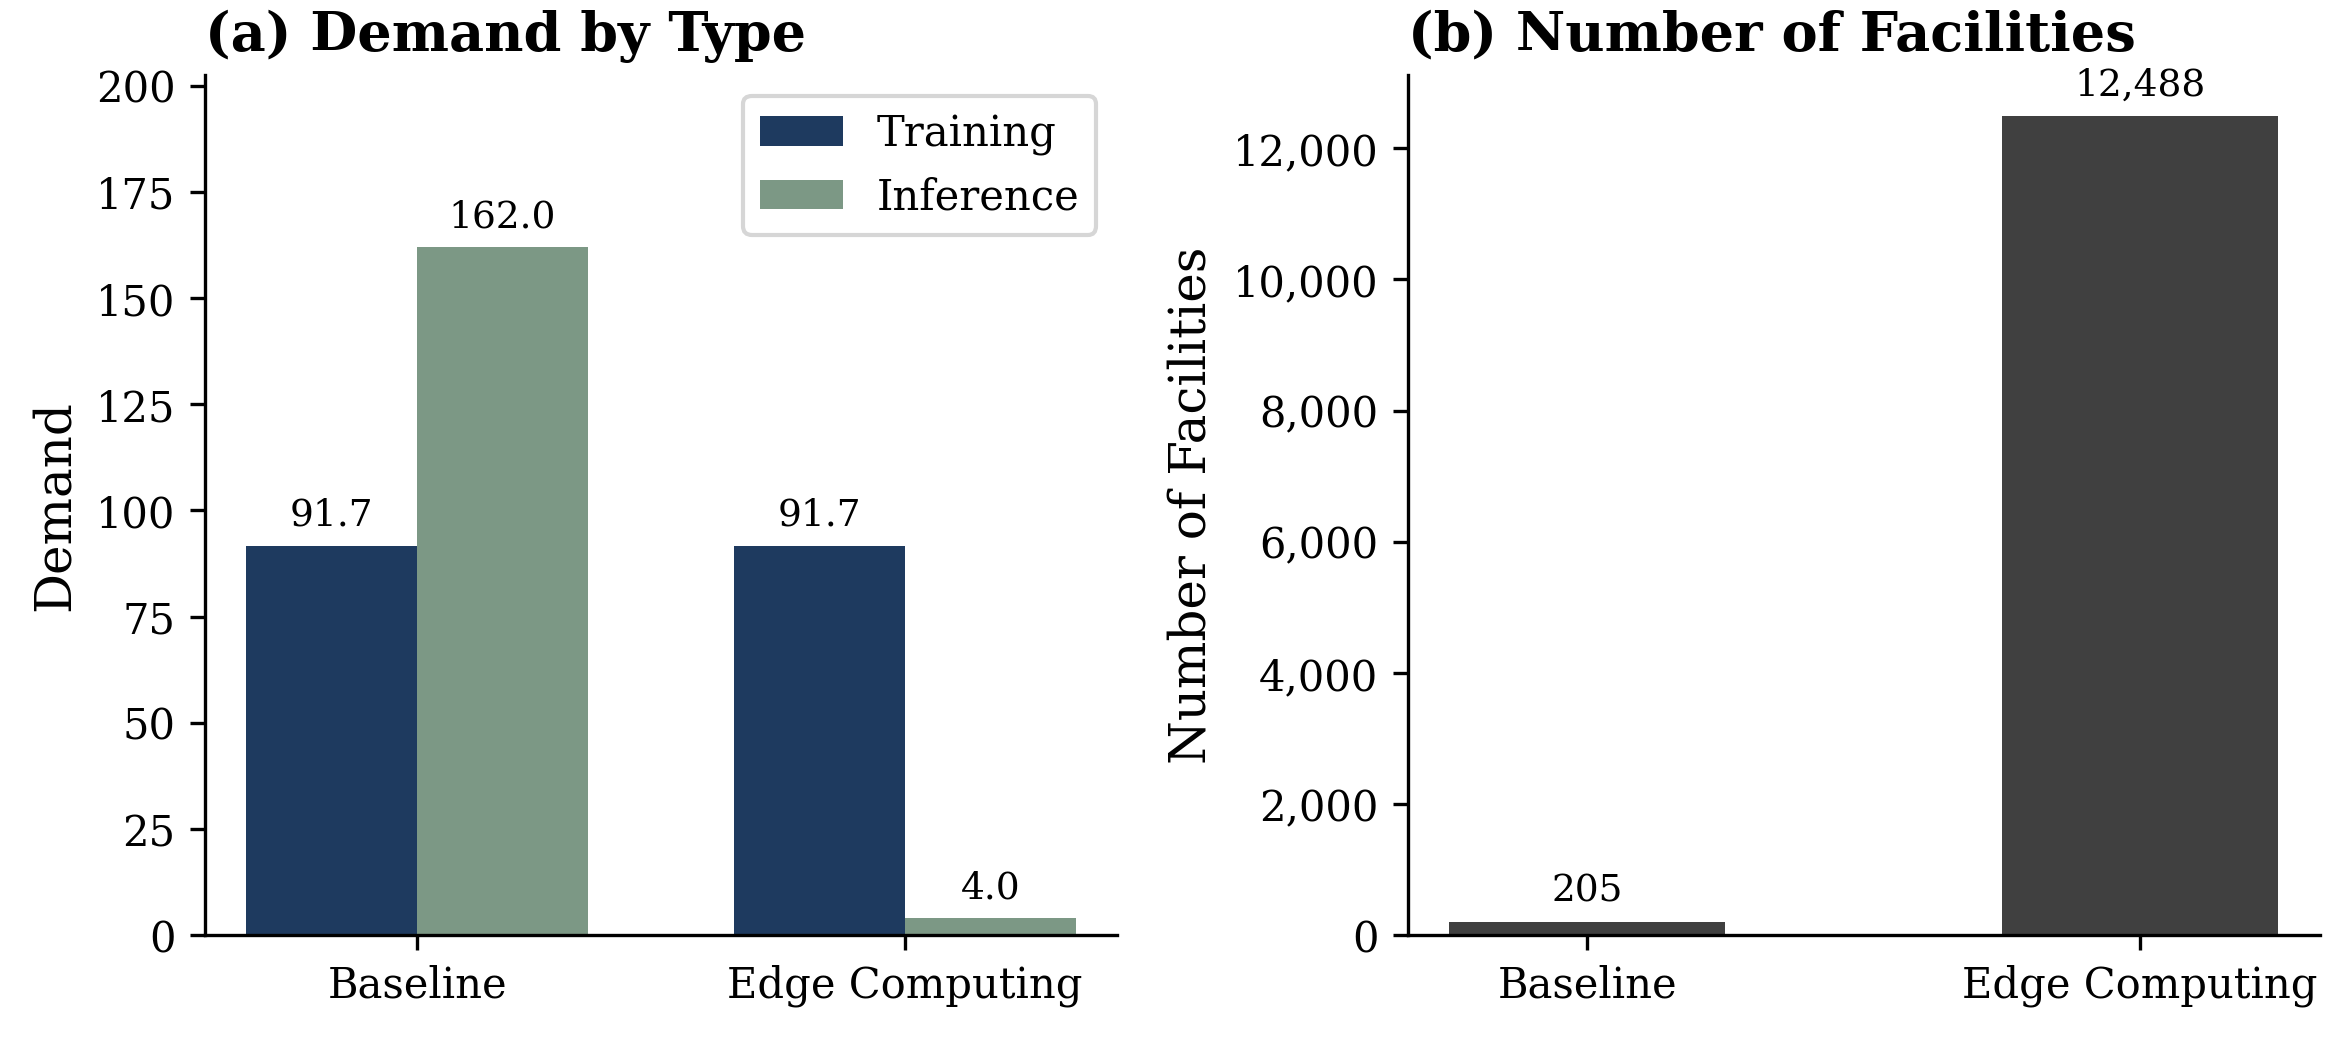
\includegraphics[width=0.5\linewidth]{Figures/CentralizedComputing.png}
%     \caption{Impact of distributing AI inference to edge data centers.}
%     \label{fig:edge_computing}
% \end{figure}

\noindent\textbf{(b) Concentration in Low-Population, High-Supply Regions.} Alternatively, we consider relocating both training and inference to regions with abundant electricity supply and lower baseline load, such as areas in the central United States with substantial renewable or fossil capacity. We simulate this by shifting demand from the baseline case where training and inference are assumed distributed to a case where the only data center for training and inference is the largest data center owned by a hyperscaler. This leads to an extreme concentration of added demand with nearly 100 GWh added near data centers in training locations. Figure~\ref{fig:CounterfactualCombined} shows this scenario.

This analysis has the important caveat that shifting to one data center for all training activity is extreme, with many possible configurations between full decentralization and full centralization. Centralization may also yield other benefits, such as concentration near renewable generation and reduced energy consumption from lower communication costs.

% \begin{figure}[h]
%     \centering
%     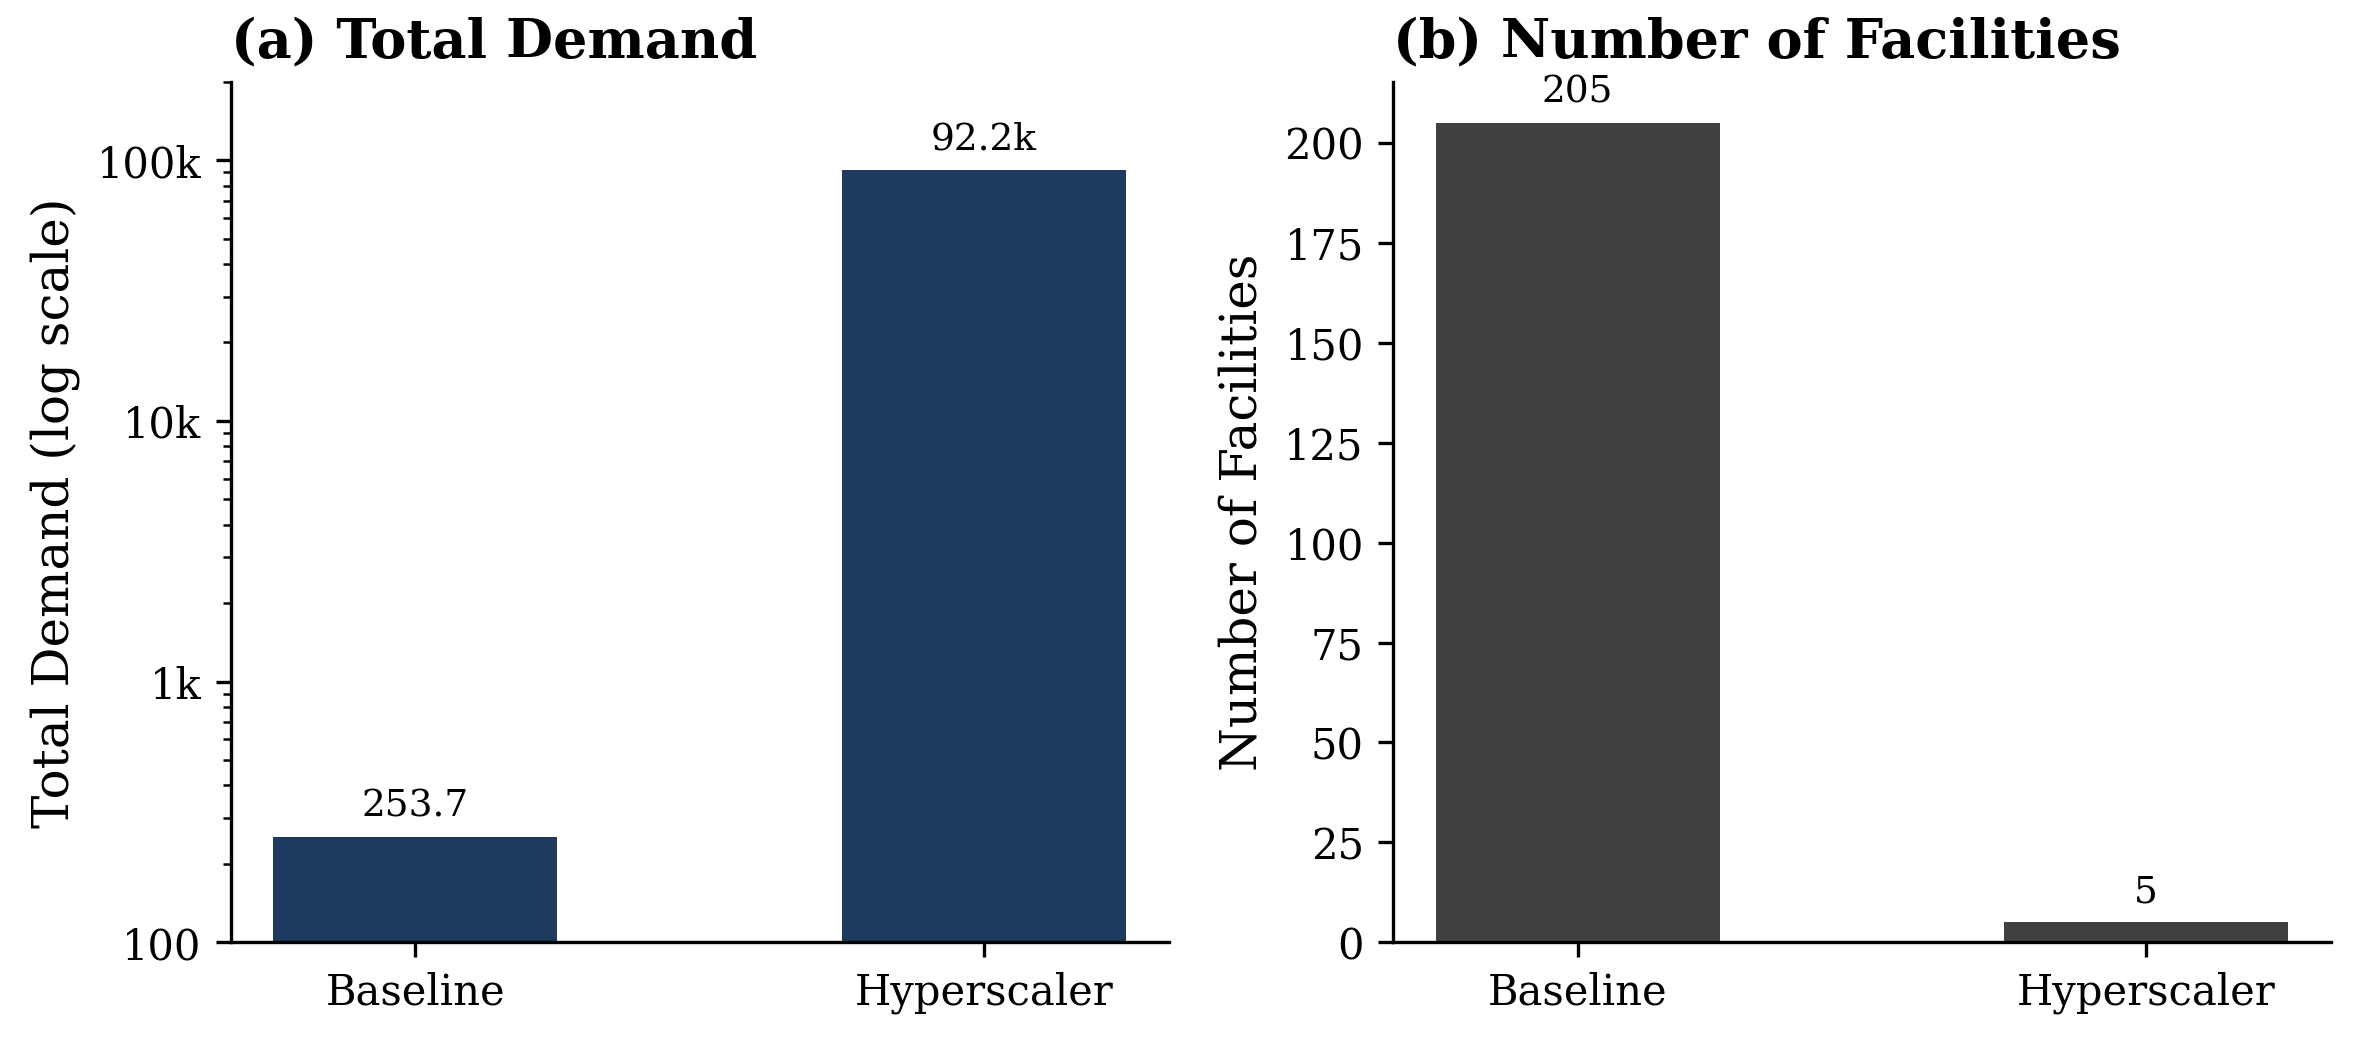
\includegraphics[width=0.5\linewidth]{Figures/Central.png}
%     \caption{Impacts of centralized computing to largest data center by hyperscaler.}
%     \label{fig:centralized_computing}
% \end{figure}

\begin{figure}
    \centering
    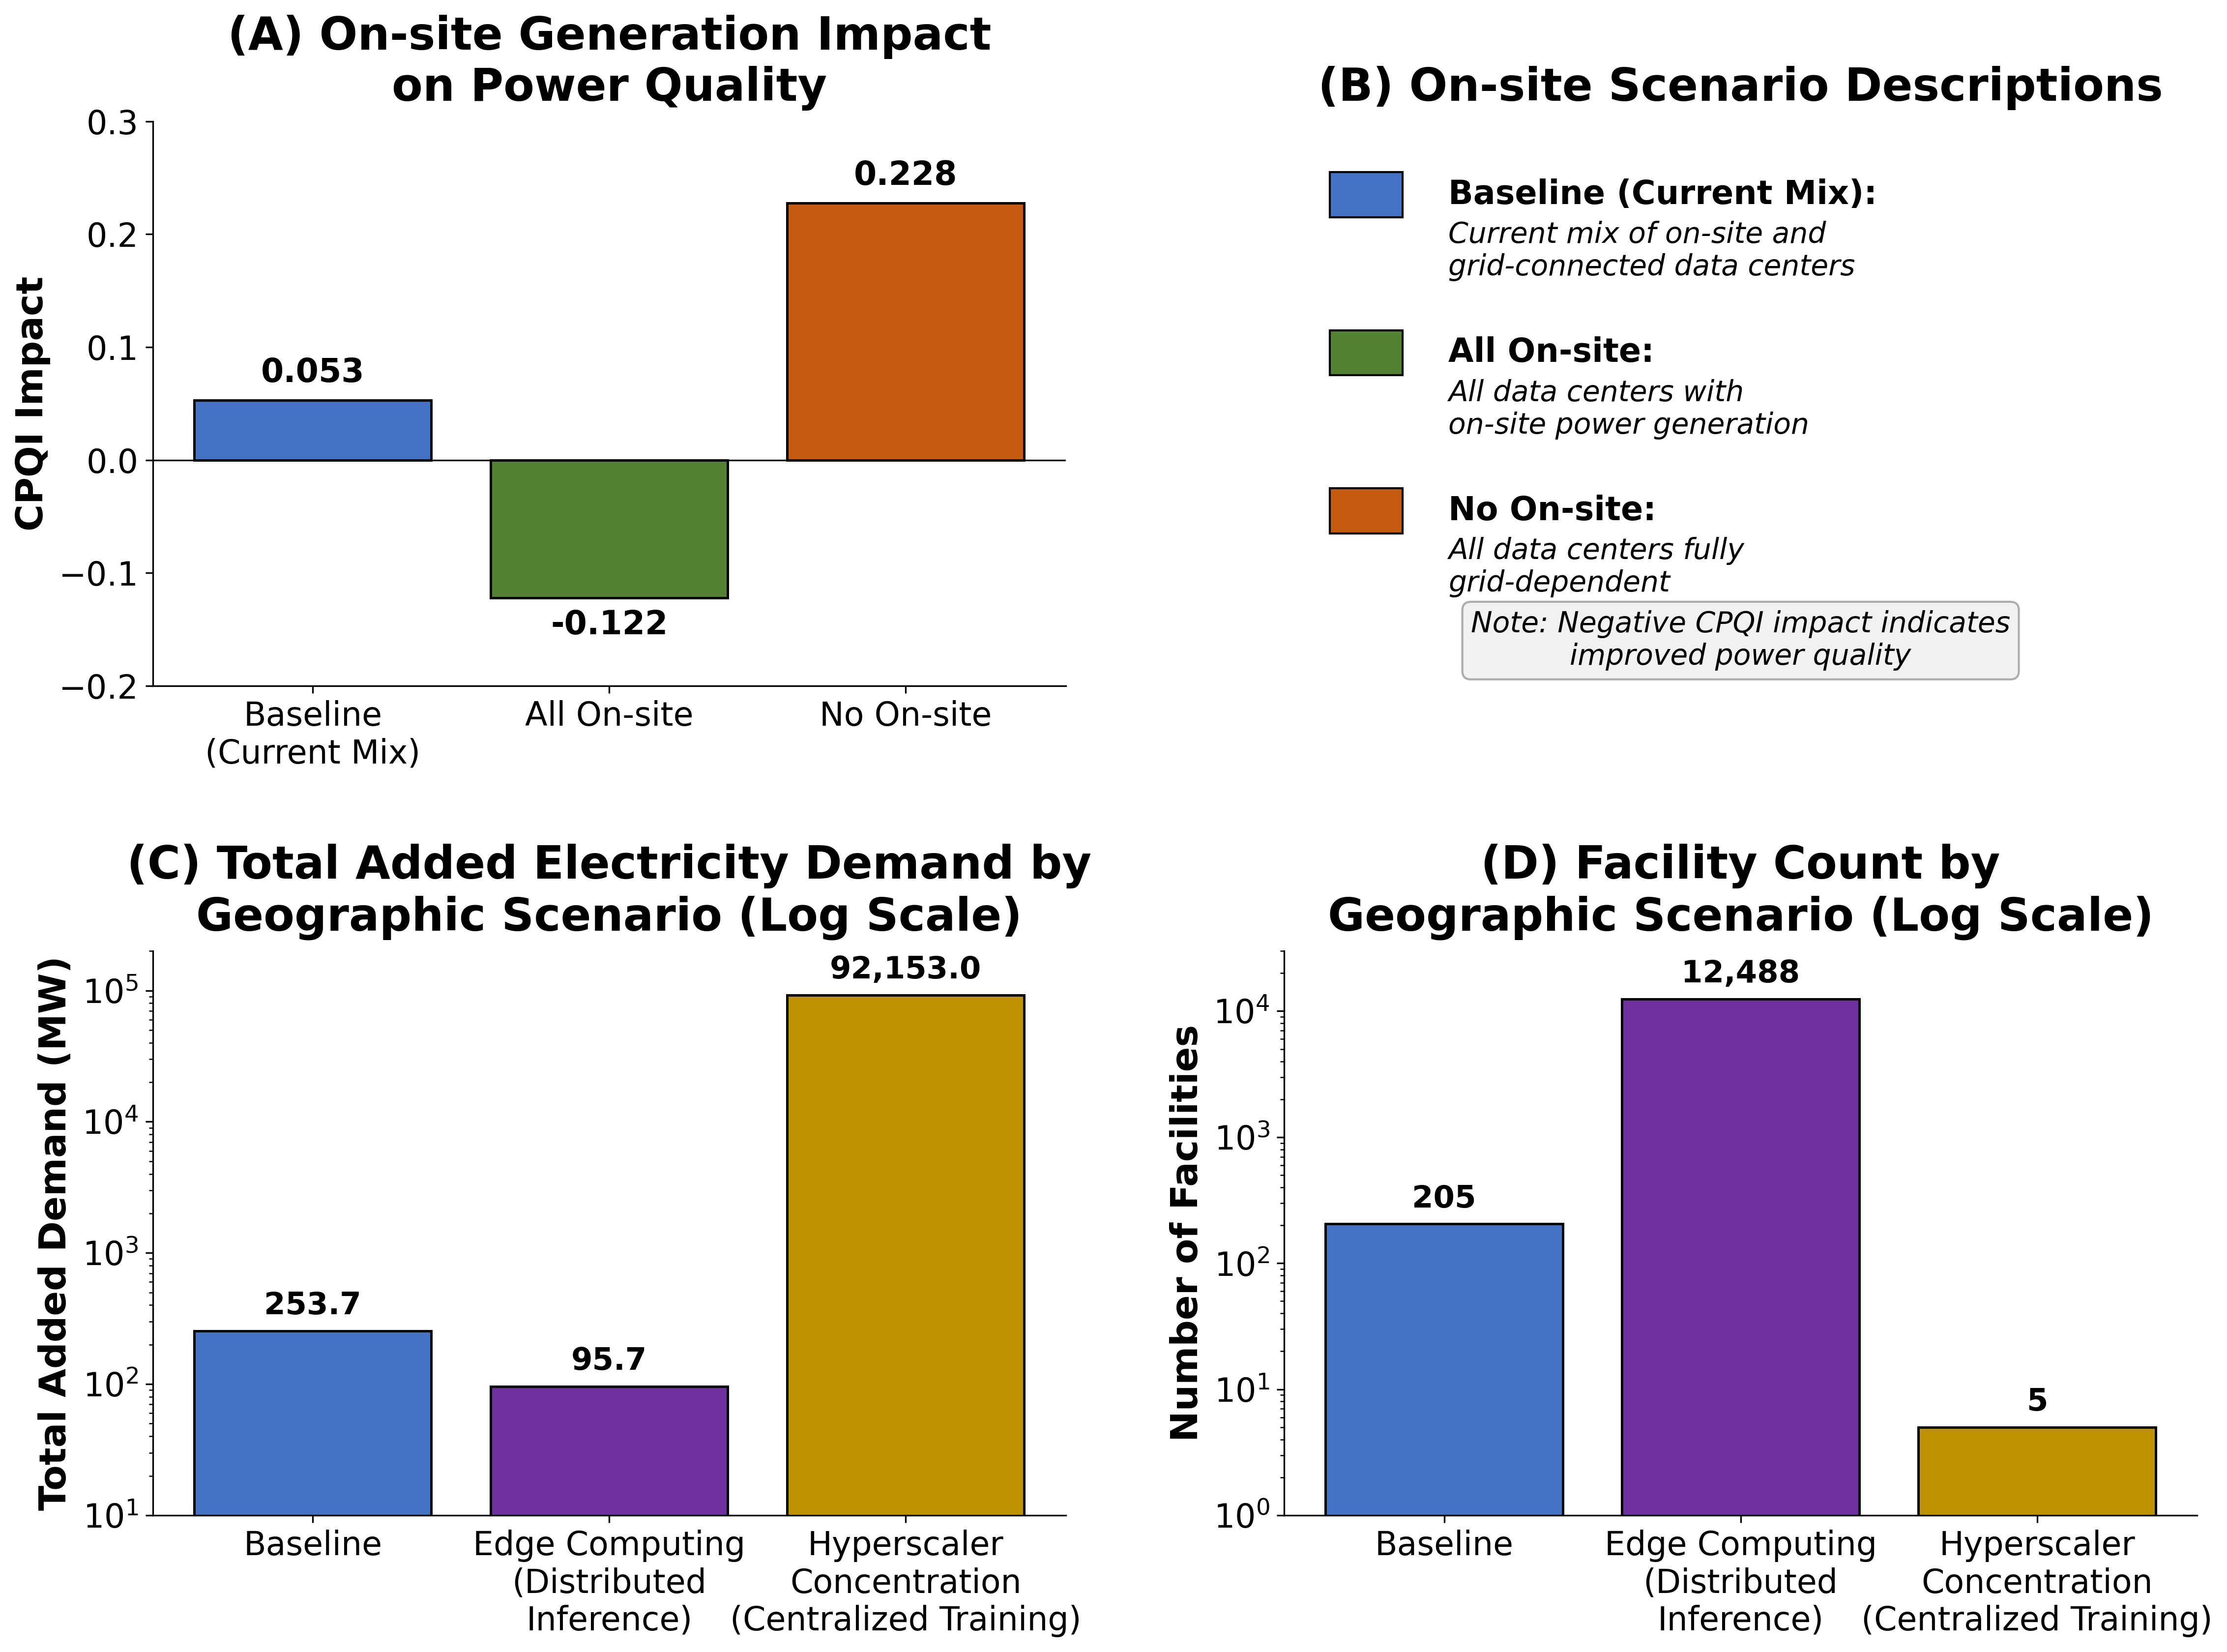
\includegraphics[width=.9\linewidth]{Figures/combined_analysis_figure.png}
    \caption{Effects of Geographic Concentration and On-site Generation on AI Impacts on the grid.}
    \label{fig:CounterfactualCombined}
    \vspace{-2em}
\end{figure}

% \subsubsection{Behind-the-Meter Power Generation Scenarios}

% One major question about the evolution of AI infrastructure concerns the role of on-site generation for data centers. To date, on-site generation investments have been relatively limited, but many investments are planned. On-site generation has numerous benefits due to the data center need for continuous direct current power with fast interconnection times and a non-smooth load profile. Significant investments in behind-the-meter power can benefit both the grid and the companies making the investments.

% We consider both a world where behind-the-meter power becomes standard and a world where on-site generation plays no role in data center power. Figure~\ref{fig:btm_scenarios} demonstrates how baseline AI impacts would change under these scenarios. Remarkably, considering only treated observations, universal adoption of BTM power would shift the impact of data centers from a net detriment to power quality to a net improvement. This suggests that data center investment in power generation substantially improves overall grid outcomes.


% \subsubsection{Additional Counterfactuals}

% Other counterfactuals could be performed with our framework, including:
% \begin{itemize}
%     \item Regressing inference coefficients on reported model queries to determine the scaling effect of additional queries on demand.
%     \item Estimating carbon emissions impacts based on the generation mix in affected regions.
%     \item Analyzing how time-of-use pricing or demand response programs might alter the temporal distribution of AI loads and associated grid impacts.
% \end{itemize}
% These extensions are left for future work.

\section{Conclusion}\label{sec:conclusion_aipower}

This paper provides the first causal estimates of how AI-driven data center demand affects U.S.\ electricity markets. Exploiting the staggered release of frontier large language models as natural experiments, we find that AI workloads cause statistically and economically significant deterioration in power quality, increase fossil fuel generation on the order of hundreds of GWh, and raise wholesale electricity prices by up to 25\% in heavily treated zones. These effects are consistent with the predictions of our game-theoretic model of hyperscaler electricity procurement, which formalizes the \emph{timing wedge}---the temporal mismatch between when data centers consume electricity and when their contracted or credited renewable generation produces.

The economic implications are substantial. The timing wedge means that the voluntary procurement instruments favored by hyperscalers---renewable energy certificates and power purchase agreements---do not internalize the externalities they are designed to address. RECs, as financial transfers unbundled from physical dispatch, leave real-time fossil generation and grid stress unaffected. PPAs improve on this margin only modestly absent firming or storage. Our counterfactual analyses reinforce this finding: universal adoption of on-site generation would reverse the sign of power quality effects, transforming data centers from a net grid liability into a net contributor. This result suggests that the externality is not inherent to AI demand per se, but rather to the spatial and temporal misalignment between that demand and clean generation---a misalignment that current market instruments fail to correct.

These findings speak directly to ongoing policy debates over renewable energy procurement design. Proposals for hourly matching, such as the 24/7 Carbon-Free Energy framework, attempt to close the timing wedge by requiring temporal alignment of clean energy credits with consumption. Our model provides a framework for evaluating such proposals: tightening matching granularity raises the effective price of RECs in high-carbon hours, increases the private value of storage, and induces entry of temporally aligned generation. The empirical heterogeneity we document between data centers with and without on-site generation offers suggestive evidence that policies promoting behind-the-meter investment could yield grid-wide benefits. Geographic redistribution of inference workloads---toward edge computing or toward high-supply, low-load regions---offers an additional policy lever, though with important tradeoffs between transmission costs and local reliability.

Our analysis has limitations. The parallel trends assumption underpinning any difference-in-differences design may be violated if treated and control regions were already diverging prior to model releases, or if generators anticipated these releases. Spillovers across interconnected regions and heterogeneous effects by grid topology or model type may attenuate or bias our estimates. Our power quality dataset, while novel, covers a limited time horizon that constrains our ability to characterize long-run trends. Finally, frontier model releases are an imperfect proxy for the continuous evolution of AI compute demand, and the mapping from a discrete release event to actual deployment and load is necessarily noisy.

Despite these limitations, the results carry clear implications for electricity market design. As AI workloads grow, regulators and system operators will need instruments that address not only the volume but the temporal and spatial profile of incremental demand. Our findings suggest that annual renewable accounting provides insufficient incentive for the investments in storage, on-site generation, and demand flexibility that would align private procurement with system-level reliability and emissions goals. The methodological approach developed here---combining econometric causal identification with publicly available grid data---is portable to other settings where proprietary operational data are unavailable, including the effects of AI on network congestion, cooling water demand, or semiconductor supply chains.

\bibliographystyle{cas-model2-names}
\bibliography{Energy}

\appendix
\section{Appendix}
\subsection{Results Tables}

\begin{table}[hbp]
\centering
\caption{Estimated Impact of AI Model Releases on Power Quality}
\label{tab:AIModelsPowerQuality}
\small
\begin{tabular}{l l r r r}
\toprule
Model & Provider & Coefficient & Std. Error & $R^{2}$ \\
\midrule
GPT-4.5                  & Microsoft   & 0.327*** & 0.087 & 0.327 \\
Llama 4 Behemoth (preview) & Facebook  & 0.325*** & 0.074 & 0.313 \\
Claude 3 Opus            & Google      & 0.278*** & 0.043 & 0.462 \\
Gemini 1.5 Pro           & Google      & 0.223*** & 0.026 & 0.451 \\
GPT-4o                   & Microsoft   & 0.198*** & 0.044 & 0.331 \\
GPT-4                    & Microsoft   & 0.176*** & 0.033 & 0.408 \\
Claude 3.7 Sonnet        & Google      & 0.161*** & 0.041 & 0.357 \\
Chinchilla               & Google      & 0.143*** & 0.038 & 0.570 \\
PaLM (540B)              & Google      & 0.142*** & 0.029 & 0.587 \\
LaMDA                    & Google      & 0.134**  & 0.044 & 0.564 \\
PaLM 2                   & Google      & 0.133*** & 0.024 & 0.465 \\
Claude 3.5 Sonnet        & Google      & 0.126*** & 0.036 & 0.378 \\
OPT-175B                 & Facebook    & 0.104*** & 0.023 & 0.467 \\
Gemini 1.0 Ultra         & Google      & 0.103*** & 0.021 & 0.409 \\
Llama 3.1-405B           & Facebook    & 0.052    & 0.034 & 0.315 \\
Minerva (540B)           & Google      & 0.031    & 0.023 & 0.519 \\
Parti                    & Google      & 0.031    & 0.023 & 0.519 \\
GPT-4 Turbo              & Microsoft   & 0.030*   & 0.017 & 0.308 \\
GPT-3.5                  & Microsoft   & -0.049** & 0.018 & 0.390 \\
Flan-PaLM 540B           & Google      & -0.051*  & 0.026 & 0.508 \\
U-PaLM (540B)            & Google      & -0.051*  & 0.026 & 0.508 \\
Amazon Titan             & Amazon AWS  & -0.086***& 0.016 & 0.380 \\
\bottomrule
\end{tabular}
\begin{flushleft}
\footnotesize
Notes: Robust standard errors in parentheses. Significance levels: *** $p<0.01$, ** $p<0.05$, * $p<0.1$.
\end{flushleft}
\end{table}

\begin{table}[htbp]\centering
\caption{Difference-in-Differences Estimates of Data Center Announcements on Cumulative Total Queue Capacity (MW)}
\begin{threeparttable}
\begin{tabular}{lcc}
\toprule
& (1) & (2) \\
& No FE & County \& Year FE \\
\midrule
Post Announcement & 714.459\sym{**} & 150.741\sym{*} \\
& (293.890) & (87.001) \\
Intercept & 366.406\sym{***} & -188.142\sym{***} \\
& (19.361) & (13.395) \\
\midrule
Observations & 128,700 & 128,700 \\
R$^2$ & 0.010 & 0.780 \\
Adj.\ R$^2$ & 0.010 & 0.777 \\
Fixed Effects & No & County \& Year \\
\bottomrule
\end{tabular}
\begin{tablenotes}[flushleft]
\footnotesize
\item Cluster-robust standard errors in parentheses. 
\item \sym{*} $p<0.10$, \sym{**} $p<0.05$, \sym{***} $p<0.01$. 
\end{tablenotes}
\end{threeparttable}
\label{DIDTotal}
\end{table}

\begin{table}[htbp]\centering
\caption{Difference-in-Differences Estimates of Data Center Announcements on Cumulative Gas Queue Capacity (MW)}
\begin{threeparttable}
\begin{tabular}{lcc}
\toprule
& (1) & (2) \\
& No FE & County \& Year FE \\
\midrule
Post $\times$ Announced Capacity & 0.324\sym{***} & 0.250\sym{**} \\
& (0.105) & (0.117) \\
Intercept & 175.718\sym{***} & -43.457\sym{***} \\
& (18.388) & (13.229) \\
\midrule
Observations & 16,380 & 16,380 \\
R$^2$ & 0.012 & 0.610 \\
Adj.\ R$^2$ & 0.012 & 0.604 \\
Fixed Effects & No & County \& Year \\
\bottomrule
\end{tabular}
\begin{tablenotes}[flushleft]
\footnotesize
\item Cluster-robust standard errors in parentheses. 
\item \sym{*} $p<0.10$, \sym{**} $p<0.05$, \sym{***} $p<0.01$. 
\end{tablenotes}
\end{threeparttable}
\label{DIDGas}
\end{table}

\begin{table}[htbp]\centering
\caption{Difference-in-Differences Estimates of Data Center Announcements on Cumulative Gas Queue Capacity (MW), No Interaction}
\begin{threeparttable}
\begin{tabular}{lcc}
\toprule
& (1) & (2) \\
& No FE & County \& Year FE \\
\midrule
Post Announcement & 98.976 & 273.893\sym{***} \\
& (68.413) & (79.284) \\
Intercept & 176.560\sym{***} & 63.585\sym{***} \\
& (18.656) & (1.28e-11) \\
\midrule
Observations & 16,380 & 16,380 \\
R$^2$ & 0.003 & 0.522 \\
Adj.\ R$^2$ & 0.002 & 0.514 \\
Fixed Effects & No & County \& Year \\
\bottomrule
\end{tabular}
\begin{tablenotes}[flushleft]
\footnotesize
\item Cluster-robust standard errors in parentheses. 
\item \sym{*} $p<0.10$, \sym{**} $p<0.05$, \sym{***} $p<0.01$. 
\end{tablenotes}
\end{threeparttable}
\label{DIDNGInteract}
\end{table}

% POST-TREATMENT EFFECTS
\begin{table}[htbp]
\centering
\caption{Post-Treatment: Estimated Impact of AI Model Releases on Aggregate Electricity Demand}
\label{tab:ai_demand_post}
\resizebox{\columnwidth}{!}{%
\begin{threeparttable}
\begin{tabular}{l l r r r r}
\toprule
Model & Provider & Coefficient & $p$-value & $R^{2}$ & Aggregate Impact (MWh) \\
\midrule
Switch                         & Google     & 124.46 & $<0.001$ & 0.628 & 4,154,379 \\
DALL\text{-}E                  & Microsoft  &  81.54 & $<0.001$ & 0.627 & 2,910,208 \\
GPT\text{-}3.5                 & Microsoft  &  76.08 & $<0.001$  & 0.622 & 1,034,517 \\
mT5\text{-}XXL                 & Google     &  63.48 & $<0.001$              & 0.625 &   420,630 \\
Megatron\text{-}Turing NLG 530B& Microsoft &  46.15 & $<0.001$  & 0.628 & 1,692,209 \\
Codex                          & Microsoft  &  35.60 & 0.0211                & 0.630 & 2,132,043 \\
Minerva (540B)                 & Google     &  24.03 & 0.4305                & 0.624 & 1,372,621 \\
Parti                          & Google     &  20.14 & 0.4692                & 0.625 & 1,183,787 \\
Flan\text{-}PaLM (540B)        & Google     &  17.36 & 0.0501                & 0.622 &   504,750 \\
U\text{-}PaLM (540B)           & Google     &  17.36 & 0.0501                & 0.622 &   504,750 \\
OPT\text{-}175B                & Facebook   &  12.85 & 0.0161                & 0.624 &   583,999 \\
ByT5\text{-}XXL                & Google     &   1.28 & 0.9584                & 0.624 &    66,424 \\
ProtT5\text{-}XXL              & Google     &  -1.42 & 0.9370                & 0.629 &   -64,268 \\
Meta Pseudo Labels             & Google     &  -3.996& 0.8284                & 0.628 &  -118,203 \\
FLAN 137B                      & Google     &  -4.97 & 0.7971                & 0.624 &  -167,480 \\
Chinchilla                     & Google     & -23.54 & 0.0980                & 0.628 &  -834,056 \\
PaLM (540B)                    & Google     & -24.53 & 0.0714                & 0.628 &  -873,641 \\
LaMDA                          & Google     & -27.41 & 0.1362                & 0.626 &  -643,963 \\
GLaM                           & Google     & -27.76 & 0.3485                & 0.625 &  -750,319 \\
Gopher (280B)                  & Google     & -30.32 & 0.3113                & 0.625 &  -813,756 \\
\bottomrule
\end{tabular}
\begin{tablenotes}
\item Notes: Coefficients and p-values are taken from \texttt{post\_coefficient} and \texttt{post\_p\_value}. Aggregate impact uses \texttt{post\_aggregate\_demand\_increase}. The headline causal claim of the chapter is the pooled stacked-DiD coefficient reported in Table~\ref{tab:combined_results}; the model-by-model rows above are reported as \emph{descriptive} per-event estimates rather than as confirmatory tests, since each row identifies off a single release event with limited statistical power. The sign pattern is consistent with the scaling story discussed in Section~\ref{sec:counterfactuals}: smaller and earlier-generation models (Chinchilla, PaLM 540B, LaMDA, Gopher 280B) carry small or negative point estimates with wide confidence bands, while larger and later-generation models (GPT-4.5, Llama 4 Behemoth, Claude 3 Opus) carry substantially larger and more precisely estimated positive coefficients. We do not interpret negative point estimates on individual older or smaller models as evidence against the AI-induced demand effect.
\end{tablenotes}
\end{threeparttable}}
\label{PostTreatment}
\end{table}

% PRE-TREATMENT EFFECTS
\begin{table}[htbp]
\centering
\caption{Pre-Treatment: Estimated Impact of AI Model Releases on Aggregate Electricity Demand}
\label{tab:ai_demand_pre}
\resizebox{\columnwidth}{!}{%
\begin{threeparttable}
\begin{tabular}{l l r r r r}
\toprule
Model & Provider & Coefficient & $p$-value & $R^{2}$ & Aggregate Impact (MWh) \\
\midrule
Switch                         & Google     &  89.77 & $<0.001$ & 0.628 &   268,851 \\
DALL\text{-}E                  & Microsoft  &  66.90 & $<0.001$ & 0.627 &    43,755 \\
GPT\text{-}3.5                 & Microsoft  &  39.60 & $<0.001$             & 0.622 & 1,501,640 \\
% mT5\text{-}XXL                 & Google     &   —    & —                    & 0.625 &      —    \\
Megatron\text{-}Turing NLG 530B& Microsoft &  35.96 & 0.0138               & 0.628 & 2,088,496 \\
Codex                          & Microsoft  &  28.63 & 0.0108               & 0.630 & 1,245,855 \\
Minerva (540B)                 & Google     & -22.51 & 0.0972               & 0.624 &  -781,775 \\
Parti                          & Google     & -22.94 & 0.1056               & 0.625 &  -734,906 \\
Flan\text{-}PaLM (540B)        & Google     &  29.16 & 0.3543               & 0.622 & 1,475,972 \\
U\text{-}PaLM (540B)           & Google     &  29.16 & 0.3543               & 0.622 & 1,475,972 \\
OPT\text{-}175B                & Facebook   & -21.77 & 0.2825               & 0.624 &  -502,990 \\
ByT5\text{-}XXL                & Google     &  -6.20 & 0.7410               & 0.624 &  -177,165 \\
ProtT5\text{-}XXL              & Google     & 101.54 & $<0.001$ & 0.629 & 3,280,303 \\
Meta Pseudo Labels             & Google     & 168.29 & $<0.001$& 0.628 & 4,122,856 \\
FLAN 137B                      & Google     &   3.41 & 0.8961               & 0.624 &    181,878 \\
Chinchilla                     & Google     & -23.61 & 0.4060               & 0.628 &  -583,230 \\
PaLM (540B)                    & Google     & -22.84 & 0.4174               & 0.628 &  -554,841 \\
LaMDA                          & Google     & -27.80 & 0.3750               & 0.626 &  -817,029 \\
GLaM                           & Google     & -12.52 & 0.4856               & 0.625 &  -413,053 \\
Gopher (280B)                  & Google     &  -8.12 & 0.6566               & 0.625 &  -271,852 \\
\bottomrule
\end{tabular}
\begin{tablenotes}
\item Notes: Coefficients and p-values are taken from \texttt{pre\_coefficient} and \texttt{pre\_p\_value}. Aggregate impact uses \texttt{pre\_aggregate\_demand\_increase}. Dashes indicate missing values in the spreadsheet. As with Table~\ref{PostTreatment}, model-by-model rows are presented as \emph{descriptive} per-event estimates rather than confirmatory tests; the chapter's identifying inference comes from the pooled stacked-DiD specification.
\end{tablenotes}
\end{threeparttable}}
\label{PreTreatment}
\end{table}

\newpage

\subsection{Expanded Dataset Description}

Below, maps can be found providing more detail on the dataset alongside tables on the datasets and the dataset sample selection criteria.

\begin{figure}[h]
    \centering
    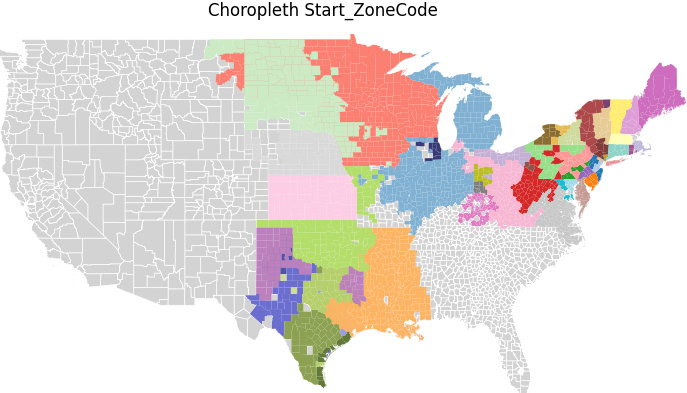
\includegraphics[width=\linewidth]{Figures/ZoneMap (1).png}
    \caption{Map of zones for demand model.}
    \label{fig:placeholder}
\end{figure}

\begin{figure}[h]
    \centering
    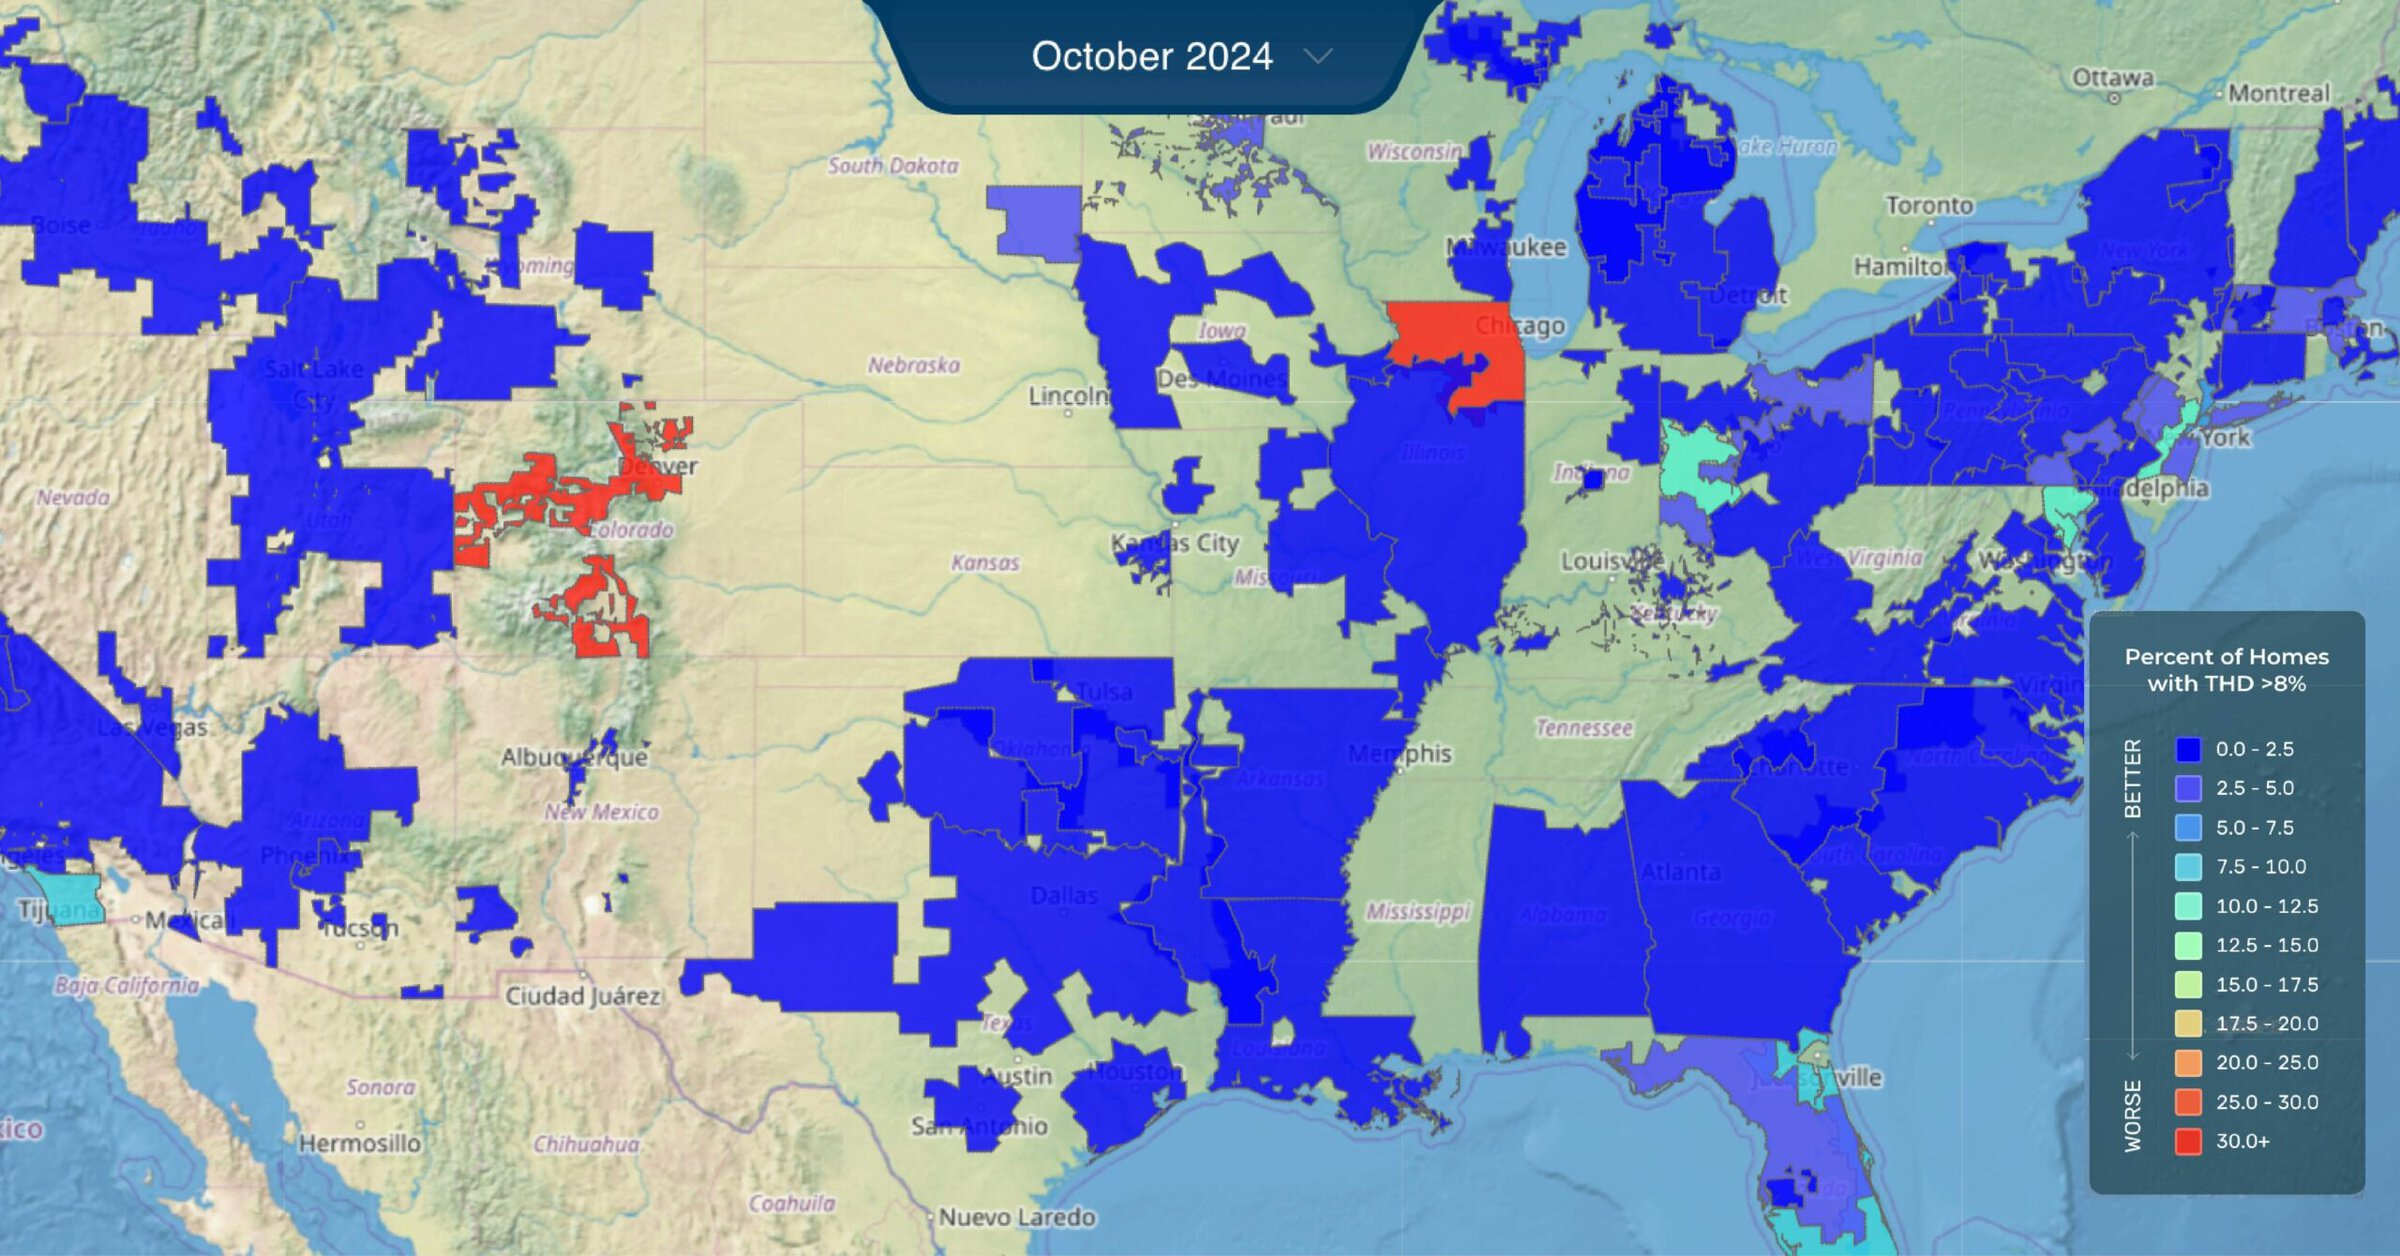
\includegraphics[width=\linewidth]{Figures/THD Dataset.jpg}
    \caption{Map of Retail Electric Utilities for Whisker Labs Data.}
    \label{fig:placeholder}
\end{figure}

\begin{figure}
    \centering
    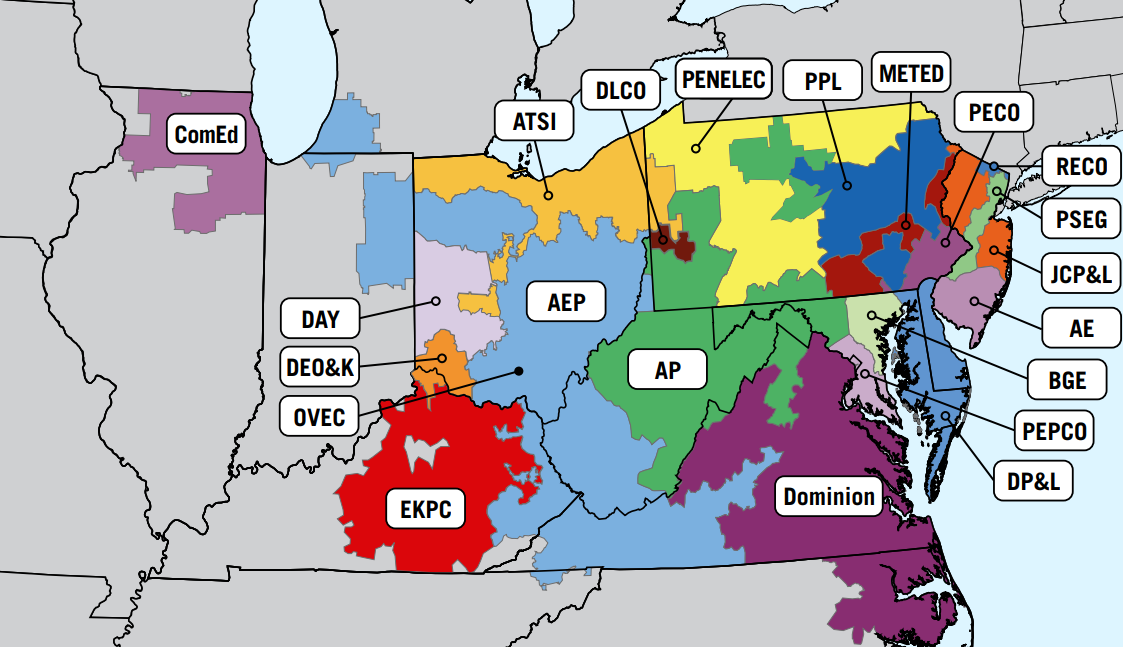
\includegraphics[width=0.75\linewidth]{Figures/PJMZonalMap.png}
    \caption{Map of PJM by Zones.}
    \label{fig:placeholder}
\end{figure}


\clearpage
\begin{sidewaystable}[p]
\centering
\caption{Expanded description of data sources (for appendix).}
\label{tab:DataSourcesExpanded}

\begin{adjustbox}{max width=\textheight} % <-- key: rotated page's usable width
\begin{threeparttable}
\begin{tabular}{p{0.18\textheight} p{0.55\textheight} p{0.25\textheight}}
\toprule
\textbf{Source} & \textbf{Content and Granularity} & \textbf{Use in Analysis} \\
\midrule
\multicolumn{3}{c}{\textbf{Q1: Difference-in-Differences (Power Quality)}} \\
\midrule
Aterio & Data center locations, establishment/expansion/retirement dates, ownership, and operational capacity (MW). Data are available at the facility level and updated annually. & Defines treatment regions; links AI model releases to hyperscaler-owned centers. \\
Whisker Labs & Consumer Power Quality Index (CPQI, composite measure of surges, sags, brownouts, interruptions) and Total Harmonic Distortion (THD, waveform distortion). Provided at county level, hourly frequency. & Outcome variables for DiD regressions. \\
Meteostat & Hourly temperature and precipitation, aggregated at the county level. Coverage includes all U.S. counties with weather stations. & Controls for demand fluctuations and renewable generation variability. \\
ISOs & Geographic boundary shapefiles and wholesale price data at zonal level. Boundaries digitized from ISO-provided maps; prices available hourly. & Market alignment and regional controls. \\
EIA & Retail service territory shapefiles, at utility level, updated periodically. & Used to define treatment/control boundaries and reconcile geographies. \\
\midrule
\multicolumn{3}{c}{\textbf{Q2: Instrumental Variables (Fossil Demand)}} \\
\midrule
EPA CAMPD & Hourly generator-level demand (MWh) and unit-specific heat rates (Btu/kWh). Coverage 2021--2023. & Generator demand is outcome; heat rates serve as instruments for prices. \\
S\&P Capital IQ & Daily natural gas price series, Henry Hub benchmark. National coverage. & Instrument for price and fuel-cost control. \\
Aterio & Generator proximity to data centers owned by releasing companies, matched at 20-mile radius. & Defines treatment generators in IV design. \\
Meteostat & Hourly temperature and precipitation, as above. & Controls for demand and renewable variability. \\
ISOs & Wholesale price series, zonal level, hourly frequency. & Market-level controls. \\
\midrule
\multicolumn{3}{c}{\textbf{Q3: Counterfactual Analyses (Scaling, Efficiency,  \& Tech Development)}} \\
\midrule
Whisker Labs & CPQI and THD (as above). Used to establish baseline deterioration in power quality. & Benchmark outcomes for scaling projections. \\
Epoch & AI model metadata: release dates, FLOPs, parameter counts. Public dataset with model-level detail. & Used for scaling regressions and efficiency counterfactuals. \\
GPU Experiments & Energy use measured on NVIDIA A6000 GPUs. Experiments run with batch size 4, sequence length 1024, and 200 inferences. Each bar in results represents total energy; lighter portion indicates communication overhead. Data collected in-house on 8xA6000 cluster. & Provides empirical GPU energy baselines for counterfactual scaling exercises. \\
\bottomrule
\end{tabular}
\end{threeparttable}
\end{adjustbox}
\end{sidewaystable}
\clearpage

\newpage
\clearpage

% 1. These two lines force the sidewaystable to center vertically on the page
\setlength{\rotFPtop}{0pt plus 1fil}
\setlength{\rotFPbot}{0pt plus 1fil}

\begin{sidewaystable}[p] % [p] forces it to be on its own page
\centering
\setlength{\tabcolsep}{3pt}
\renewcommand{\arraystretch}{0.95}

\caption{Dataset sample selection and summary statistics}
\label{tab:SampleSelection}

\begin{threeparttable}
\footnotesize
% 2. Use \linewidth so it fills the text block, but relies on margins for centering
\begin{tabularx}{\linewidth}{lXl} 
\toprule
\textbf{Dataset} & \textbf{Content / Summary Statistics} & \textbf{Sample Selection} \\
\midrule
Aterio & Data center locations, ownership, and capacity; mapped to ISO zones, EIA service territories, and counties & Hyperscaler data centers (Meta, Microsoft, Amazon, Google; Anthropic via Google) \\
\midrule
Whisker Labs & Reliability measures: CPQI ($N=2{,}683$, mean=0.52, s.d.=0.42); THD (mean=1.81, s.d.=6.77) & 72 retail electric utilities, monthly data 2022--2025 \\
\midrule
CAMPD & Generator-level demand: mean 218 MW (s.d.=158); operating times $\approx 1$ & Several thousand fossil generators, hourly data 2021--2023 \\
\midrule
ISOs & Wholesale electricity prices: mean $\$51$/MWh (s.d.=148); zonal boundaries & Deregulated markets in Eastern Interconnection and ERCOT \\
\midrule
Weather (Meteostat) & Temperature (mean=17°C, s.d.=11.4); precipitation (mean=0.12 mm, s.d.=0.91) & Matched by county/zone, hourly or daily resolution \\
\midrule
External Controls & Natural gas prices, ISO market data, geography/time harmonization & Used for both DiD and IV regressions \\
\bottomrule
\end{tabularx}

\begin{tablenotes}
\scriptsize
\item Notes: Time series are harmonized at hourly or monthly resolution depending on source. Unified panel supports both difference-in-differences (power quality) and instrumental variable (demand) regressions. Maps of sample regions provided in the appendix.
\end{tablenotes}
\end{threeparttable}

\end{sidewaystable}
\clearpage
\newpage

\subsection{Dataset Creation Diagram}

\begin{figure}[htbp]
\centering
\begin{tikzpicture}[
    scale=0.72,
    transform shape,
    node distance=0.48cm and 0.7cm,
    % === STYLES ===
    source/.style={
        cylinder,
        shape border rotate=90,
        draw=#1!60!black,
        fill=#1!12,
        text centered,
        minimum height=1.55em,
        minimum width=1.6cm,
        aspect=0.35,
        font=\tiny,
        align=center
    },
    source/.default=green,
    process/.style={
        rectangle,
        draw=blue!50!black,
        fill=blue!10,
        text centered,
        rounded corners=2pt,
        minimum height=1.35em,
        minimum width=1.8cm,
        font=\tiny,
        align=center
    },
    model/.style={
        rectangle,
        draw=#1!60!black,
        fill=#1!12,
        thick,
        text centered,
        rounded corners=3pt,
        minimum height=1.85em,
        minimum width=2.4cm,
        font=\scriptsize\bfseries,
        align=center
    },
    model/.default=red,
    arrow/.style={
        -{Stealth[scale=0.65]},
        semithick,
        color=gray!70!black
    },
    directarrow/.style={
        -{Stealth[scale=0.55]},
        color=blue!50!black,
        thin
    },
    grouplabel/.style={
        font=\tiny\bfseries,
        color=gray!70!black
    },
    annot/.style={
        font=\scriptsize,
        color=gray!60!black
    }
]

% === COLUMN 1: DATA SOURCES ===

% AI/Data Center Data (green shades)
\node[source=green!80!black] (aterio) {Aterio};

% Power Quality Data (teal shades)
\node[source=teal, below=0.35cm of aterio] (whisker) {Whisker Labs};

% Generator/Market Data (blue shades)
\node[source=blue!70!black, below=0.35cm of whisker] (campd) {EPA CAMPD};
\node[source=blue!70!black, below=0.26cm of campd] (spiq) {S\&P Capital IQ};
\node[source=blue!70!black, below=0.26cm of spiq] (isos) {ISOs};

% Government/Geographic (cyan shades)
\node[source=cyan!70!black, below=0.35cm of isos] (eia) {EIA};

% Weather (blue-green shades)
\node[source=blue!60!green, below=0.35cm of eia] (weather) {Meteostat};

% AI Model Data (purple shades)
\node[source=purple, below=0.35cm of weather] (epoch) {Epoch};

% === COLUMN 2: DATA CONSTRUCTION STEPS ===

% Treatment Definition
\node[process, right=1.5cm of aterio, yshift=-0.3cm] (treat_def) {Treatment\\Definition};

% Outcome Construction
\node[process, right=1.5cm of whisker, yshift=-0.2cm] (outcome_pq) {Power Quality\\Outcomes};

% Fossil Demand Construction
\node[process, right=1.5cm of campd, yshift=-0.3cm] (fossil_dem) {Fossil Demand\\Outcomes};

% Instrument Construction
\node[process, right=1.5cm of isos, yshift=0.1cm] (instruments) {Instruments \&\\Controls};

% Service Territory Mapping
\node[process, right=1.5cm of eia] (territory) {Service Territory\\Mapping};

% Scaling Data
\node[process, right=1.5cm of epoch] (scaling) {Scaling\\Regressions};

% === COLUMN 3: ANALYSIS MODELS ===

% Q1: DiD Model
\node[model=orange, right=3.2cm of outcome_pq, yshift=0.8cm] (q1) {Q1: Difference-in-\\Differences};

% Q2: IV Model  
\node[model=red, below=0.7cm of q1] (q2) {Q2: Instrumental\\Variables};

% Q3: Counterfactual Model
\node[model=violet, below=0.7cm of q2] (q3) {Q3: Counterfactual\\Analyses};

% === CONNECTIONS ===

% To Treatment Definition
\draw[arrow] (aterio.east) -- (treat_def.west);

% To Power Quality Outcomes
\draw[arrow] (whisker.east) -- (outcome_pq.west);

% To Fossil Demand Outcomes
\draw[arrow] (campd.east) -- (fossil_dem.west);

% To Instruments & Controls
\draw[arrow] (spiq.east) -- ++(0.35,0) |- (instruments.170);
\draw[arrow] (isos.east) -- (instruments.west);
\draw[arrow] (weather.east) -- ++(0.35,0) |- (instruments.190);

% To Service Territory Mapping
\draw[arrow] (eia.east) -- (territory.west);

% To Scaling Regressions
\draw[arrow] (epoch.east) -- (scaling.west);

% === CONNECTIONS TO MODELS ===

% Q1 connections
\draw[arrow] (treat_def.east) -- ++(0.2,0) |- (q1.170);
\draw[arrow] (outcome_pq.east) -- ++(0.3,0) |- (q1.west);
\draw[arrow] (territory.east) -- ++(0.4,0) |- (q1.210);

% Q2 connections
\draw[arrow] (treat_def.east) -- ++(0.5,0) |- (q2.130);
\draw[arrow] (fossil_dem.east) -- ++(0.2,0) |- (q2.170);
\draw[arrow] (instruments.east) -- ++(0.15,0) |- (q2.west);

% Q3 connections
\draw[arrow] (outcome_pq.east) -- ++(0.6,0) |- (q3.130);
\draw[arrow] (scaling.east) -- ++(0.2,0) |- (q3.west);

% Direct data feeds
\draw[directarrow] (aterio.east) -- ++(5.3,0) |- (q2.50);
\draw[directarrow] (whisker.east) -- ++(5.5,0) |- (q3.50);

% === BACKGROUND GROUPINGS ===
\begin{scope}[on background layer]
    % Raw Data Sources
    \node[fit=(aterio)(epoch), 
          fill=gray!7, 
          rounded corners=3pt, 
          draw=gray!30,
          inner sep=4pt] (rawbox) {};
    \node[grouplabel, above=0.02cm of rawbox.north] {Data Sources};
    
    % Data Construction
    \node[fit=(treat_def)(scaling)(territory)(instruments), 
          fill=blue!5, 
          rounded corners=3pt, 
          draw=blue!20,
          inner sep=5pt] (constructbox) {};
    \node[grouplabel, above=0.02cm of constructbox.north] {Variable Construction};
    
    % Models
    \node[fit=(q1)(q2)(q3), 
          fill=red!5, 
          rounded corners=3pt, 
          draw=red!20,
          inner sep=5pt] (modelbox) {};
    \node[grouplabel, above=0.02cm of modelbox.north] {Estimation};
\end{scope}

% === ANNOTATIONS ===
% Observation counts
\node[font=\fontsize{4}{5}\selectfont, color=gray!50!black, below=0.08cm of rawbox.south, text width=2.6cm, align=center] 
    {3,862 data centers\\22M generator-hours\\2,684 utility-months};

% Model annotations
\node[annot, right=0.08cm of q1.east] {\tiny Power Quality};
\node[annot, right=0.08cm of q2.east] {\tiny Fossil Demand};
\node[annot, right=0.08cm of q3.east] {\tiny AI Technical Evolution};

\end{tikzpicture}
\caption{Data sources and analysis pipeline. Data sources flow through variable construction into three estimation strategies addressing power quality impacts (Q1), fossil fuel demand (Q2), and counterfactual scaling scenarios (Q3).}
\label{fig:DataDiagram}
\end{figure}

\subsection{Construction of Zonal Geographic Maps}\label{zonalMappingEfforts}


A central requirement of the analysis is the ability to match generators to geographic areas in a manner consistent with ISO market structure while preserving as much spatial detail as possible. Because publicly available GIS shapefiles for ISO-defined market zones are incomplete, inconsistent, or entirely unavailable, the construction of zonal maps required substantial manual effort. I view this process as a significant contribution of the paper.

The guiding principle throughout was to aggregate only where necessary to permit consistent geographic matching and econometric analysis, while keeping the data at the lowest feasible spatial resolution. In all cases, zonal boundaries were explicitly restricted to lie within ISO boundaries using GIS shapefiles defining Independent System Operator footprints. This prevents generators, loads, or weather observations from being incorrectly assigned across ISOs.

\paragraph{General Approach.}
The mapping procedure proceeds in three steps. First, ISO boundaries are imposed as a hard geographic constraint. Second, ISO-specific zones are mapped to counties or county aggregates using a combination of published documentation, utility maps, and GIS overlays. Third, generators are assigned to zones using EIA Form 860 identifiers where available, and county-level geographic matching otherwise. Hand-constructed crosswalk tables are used to reconcile inconsistent geographic schemas across datasets.

Where counties do not align cleanly with ISO zones, counties are split proportionally based on geographic overlap and engineering judgment, applied consistently across datasets.

\paragraph{ERCOT.}
For ERCOT, zones are based primarily on the system’s published weather zones, which in most cases map cleanly to county boundaries. Where weather zones do not align perfectly with counties, I split counties across zones using GIS overlays to preserve contiguity and proportional area. Several ERCOT datasets rely on alternative geographic schemas (e.g., hub- or region-based reporting); in these cases, I construct hand-built mapping tables to reconcile these schemas with the zonal structure used in the analysis.

\paragraph{PJM.}
PJM required the most extensive manual mapping effort. PJM publishes a large number of zones, many of which do not correspond cleanly to county boundaries. I manually mapped each PJM zone to counties using a combination of PJM documentation, utility service maps, and GIS inspection. In cases where counties span multiple PJM zones, judgment was applied to split counties as cleanly as possible while preserving geographic continuity. Where appropriate for the analysis, zones were subsequently aggregated into regions to support the distribution of generation data.

\paragraph{SPP.}
SPP zones were mapped using a similar procedure, combining transmission zone definitions with county-level utility maps and GIS shapefiles. In several states, publicly available utility maps with county labels were used to guide assignments. As with PJM, counties were split only where necessary, and always within ISO boundaries.

\paragraph{NYISO.}
For NYISO, zones were mapped based on reliability assessment zones using a zonal county map. These zones align relatively well with county boundaries, allowing for a clean assignment in most cases.

\paragraph{MISO.}
MISO presents a comparatively clean case: all zonal boundaries correspond to state-level regions. As a result, counties were assigned directly to MISO zones based on state boundaries, eliminating the need for county splitting.

\paragraph{ISO New England.}
ISO New England zones are primarily defined at the state level, with the notable exception of Massachusetts, which is divided into three wholesale zones. For Massachusetts, I manually mapped counties to zones using GIS overlays and ISO documentation, splitting counties where necessary to maintain geographic consistency.

\paragraph{Generator Assignment.}
Generators are assigned to zones using ISO labels from EIA Form 860 wherever possible, which minimizes the risk of misassignment across ISOs. When ISO labels are unavailable or insufficiently granular, generators are matched using county-level geographic information derived from plant location data. This layered approach ensures consistency between generator assignment, zonal geography, and ISO market structure.

Overall, this mapping procedure enables the construction of consistent zonal maps that balance geographic precision with analytical tractability, forming the backbone of the spatial analysis in the paper.

\subsection{Counterfactual}
Figure \ref{fig:counterQuality} shows the power quality line we fit for performing counterfactuals.

\begin{figure}[h]
    \centering
    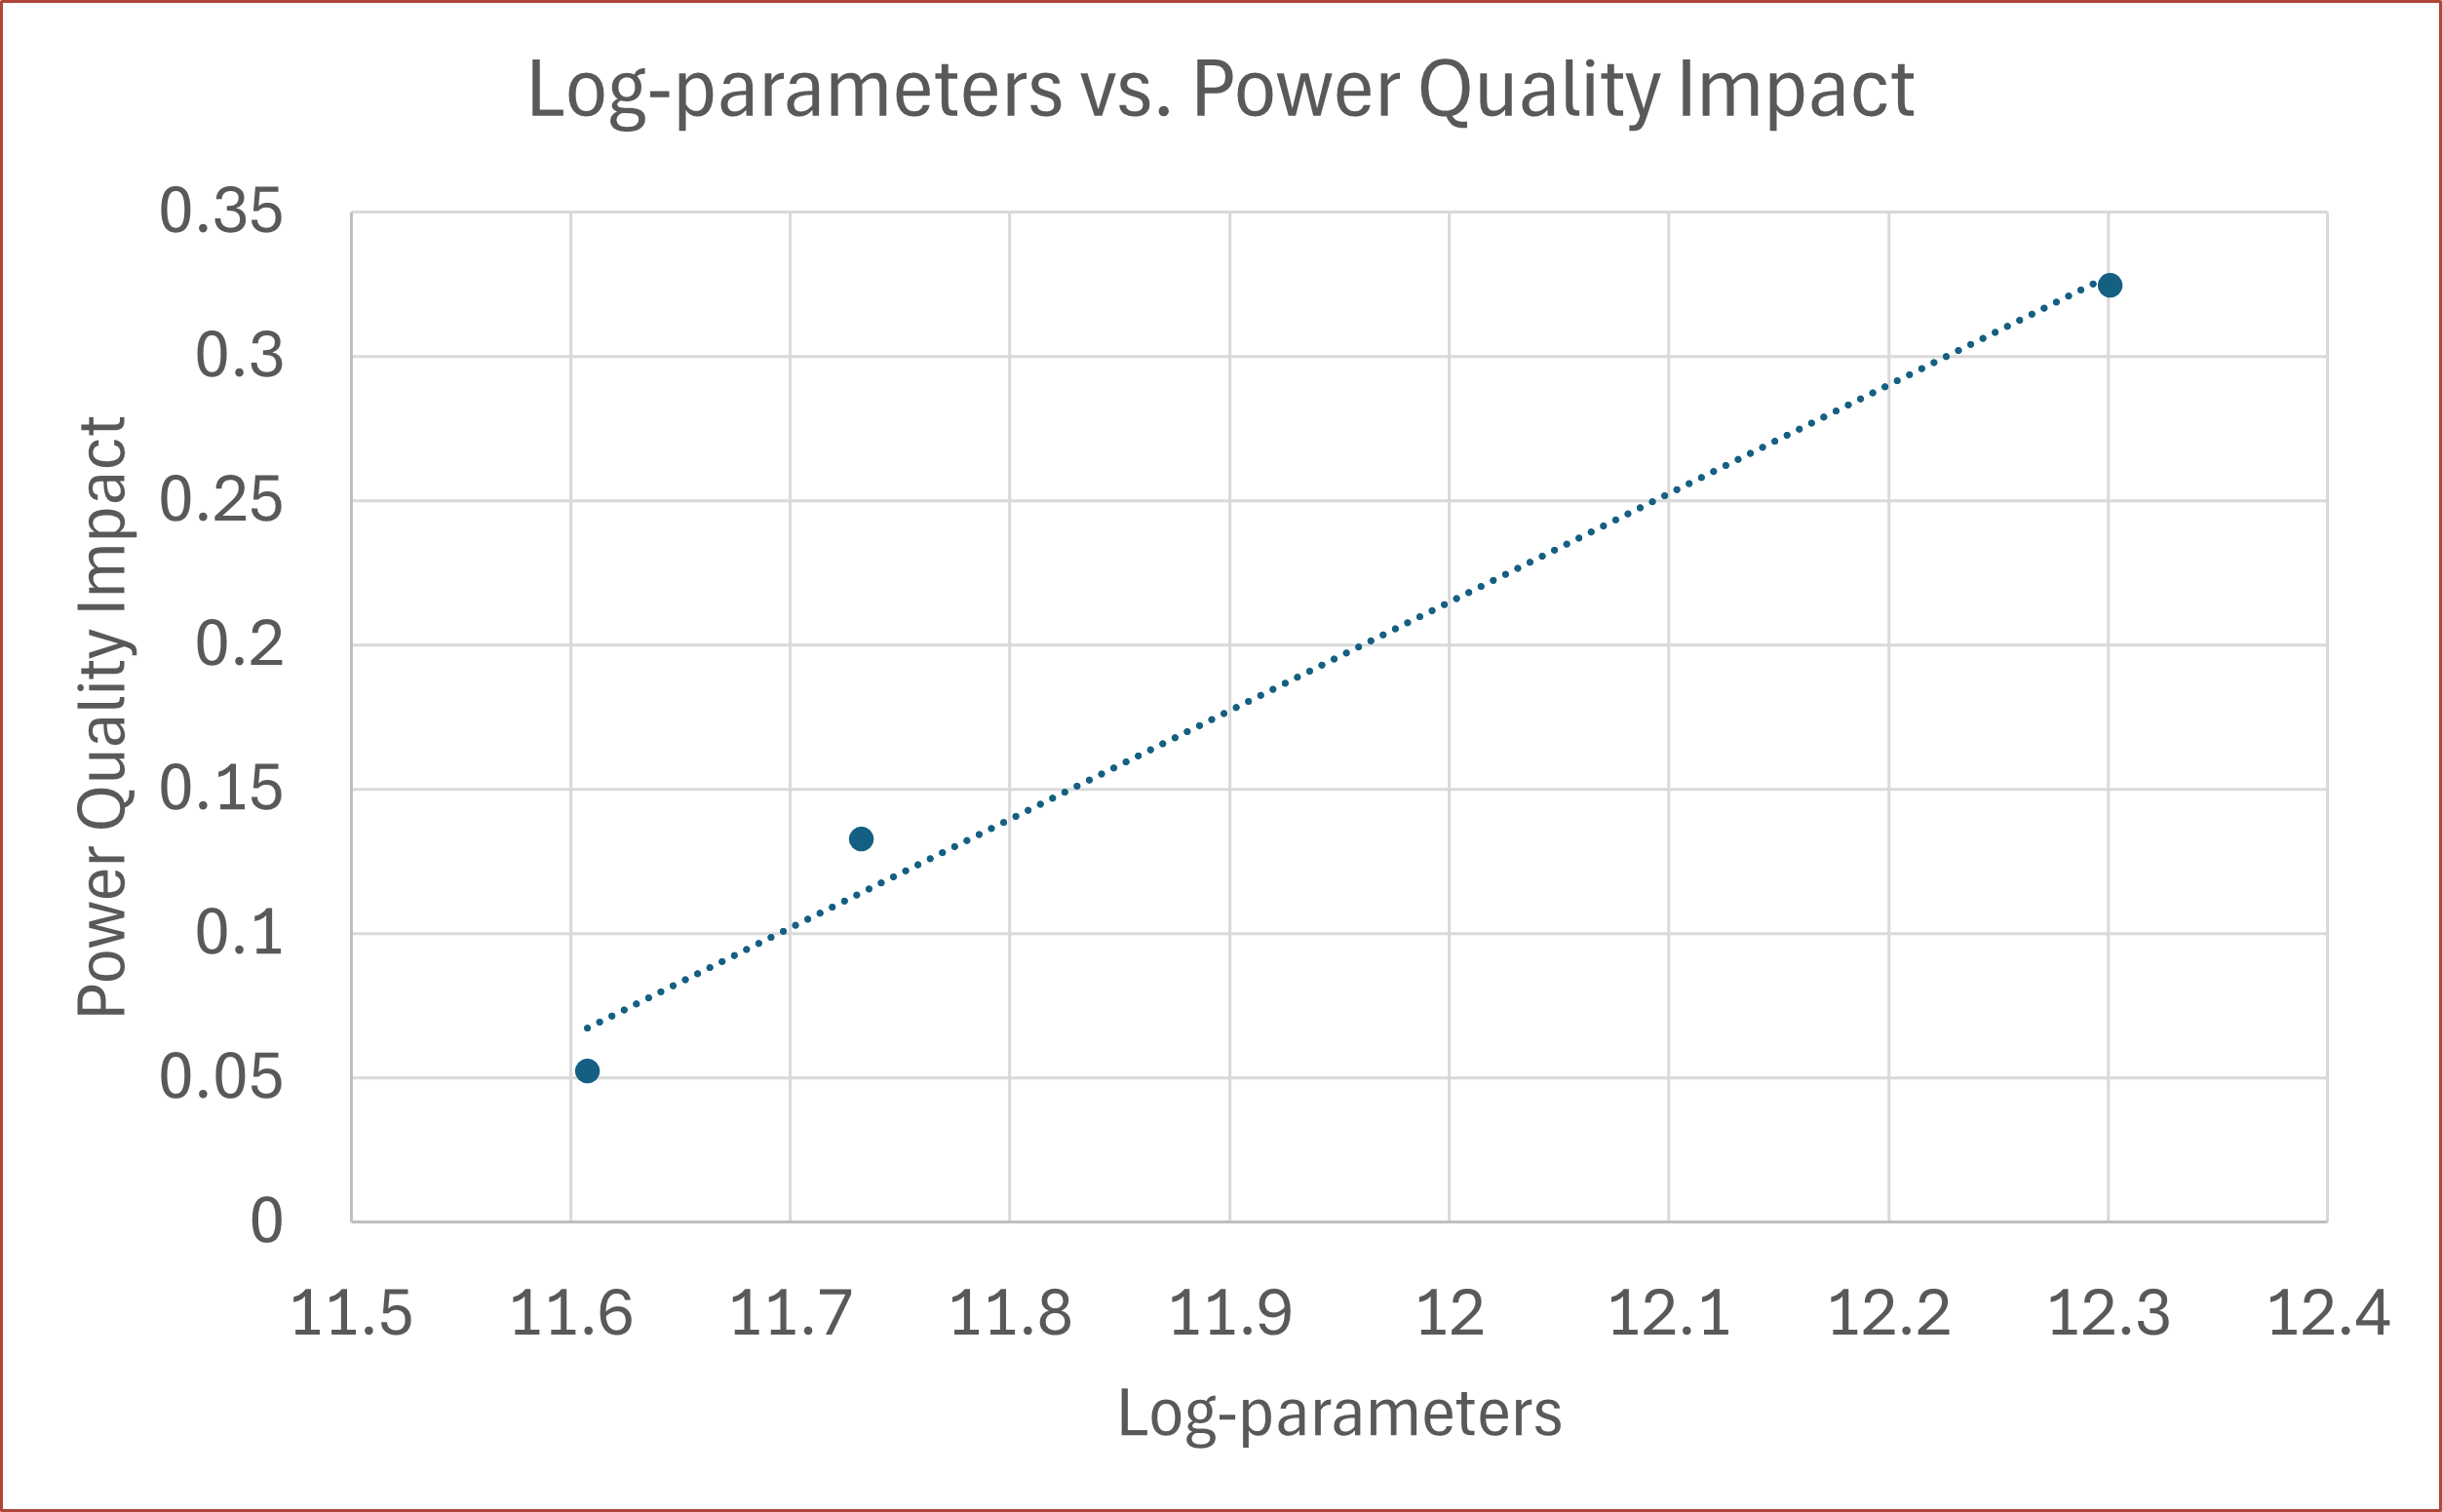
\includegraphics[width=0.5\linewidth]{Figures/Power Quality Impact1.png}
    \caption{Power Quality Impact for Counterfactuals.}
    \label{fig:counterQuality}
\end{figure}

\subsection{Calculation of Comparisons}

We calculate the household average energy usage based on data provided by \cite{USHouseholdConsumption}. We simply divide our estimates by the provided numbers to get the number of households for our comparisons.

\subsection{Code and Replication}
\label{appendix:replication}

This appendix provides comprehensive documentation for replicating the empirical analysis. All code and data processing scripts are available in the supplementary materials.

\subsubsection{Software Requirements}
\label{appendix:software}

The analysis pipeline is implemented in Python 3.11 and designed to execute on a Linux HPC cluster using the SLURM workload manager. Scripts include environment-aware path detection to support local execution on Windows systems.

\paragraph{Computational Resources.} The full pipeline requires approximately 32GB of memory and 8 CPU cores, with an expected runtime of 12--24 hours on an HPC cluster (24--48 hours for local execution). Memory-intensive operations include spatial joins for utility service territory matching and construction of stacked difference-in-differences datasets.

\paragraph{Python Dependencies.} The analysis requires the following packages: \texttt{pandas} ($\geq$2.0), \texttt{numpy} ($\geq$1.24), \texttt{scipy} ($\geq$1.10), \texttt{statsmodels} ($\geq$0.14), \texttt{linearmodels} ($\geq$5.0), \texttt{geopandas} ($\geq$0.14), \texttt{shapely} ($\geq$2.0), \texttt{fiona} ($\geq$1.9), \texttt{pyproj} ($\geq$3.6), \texttt{rtree} ($\geq$1.0), \texttt{geopy} ($\geq$2.3), \texttt{gdal} ($\geq$3.6), \texttt{matplotlib} ($\geq$3.7), and \texttt{seaborn} ($\geq$0.12). We use \texttt{micromamba} for environment management on the cluster.

\subsubsection{Data Sources}
\label{appendix:data}

Table~\ref{tab:data_sources} summarizes the primary data sources used in the analysis. All data files should be placed in a \texttt{Data/} subdirectory relative to the code directory.

\begin{table}[htbp]
\centering
\caption{Data Sources and Descriptions}
\label{tab:data_sources}
\footnotesize % Reduces font size slightly to fit narrow columns
% @{} removes extra side padding to maximize space
% >{\raggedright\arraybackslash}X wraps text and left-aligns it
\begin{tabularx}{\columnwidth}{@{} >{\raggedright\arraybackslash}X >{\raggedright\arraybackslash}X l @{}}
\toprule
\textbf{File} & \textbf{Description} & \textbf{Source} \\
\midrule
\multicolumn{3}{l}{\textit{Electricity Demand Analysis}} \\
\texttt{EPAData.csv} & Hourly emissions and generation & EPA CAMPD \\
\texttt{epa\_eia\_crosswalk.csv} & EPA--EIA facility identifiers & Custom \\
\texttt{data\_center\_inventory.csv} & Data center locations with AI flags & Aterio \\
\texttt{mapData.shp} & Zone boundary shapefiles & FERC/ISO \\
\texttt{TransmissionPriceLoad.csv} & Zonal electricity prices and load & ISO/RTO \\
\texttt{ExtendedNGPriceData.csv} & Natural gas price time series & EIA \\
\texttt{mapDatawithWeather.csv} & Zone-level weather data & NOAA \\
\midrule
\multicolumn{3}{l}{\textit{Power Quality Analysis}} \\
% Manually broke this long filename to ensure it fits the column
\texttt{electric-retail-service- \newline territories.shp} & Utility service area boundaries & EIA-861 \\
\texttt{Epoch Database - Notable Models.csv} & AI model release dates & Epoch AI \\
\texttt{PowerQuality.csv} & Customer Power Quality Index & Whisker Labs \\
\texttt{THD.csv} & Total Harmonic Distortion & PQ Monitor \\
\midrule
\multicolumn{3}{l}{\textit{Robustness Checks}} \\
\texttt{ai\_model\_dates\_verified.csv} & Verified API release dates & Manual \\
\bottomrule
\end{tabularx}
\end{table}

\subsubsection{Pipeline Architecture}
\label{appendix:pipeline}

The analysis executes in four sequential phases, with internal parallelization within phases. Figure~\ref{fig:pipeline} illustrates the data flow.

\paragraph{Phase 1: Data Construction.} The script \texttt{CreateDataIVDiffinDiffCAMPD.py} constructs the panel dataset by merging EPA emissions data with data center locations, electricity market data, and natural gas prices. Key variables created include: \texttt{treated} (binary indicator for zones within proximity of AI data centers), \texttt{post} (binary indicator for post-AI-model-release periods), and \texttt{treatment\_intensity} (continuous measure based on model compute requirements). Output: \texttt{panelIVDiDData.csv}.

\paragraph{Phase 2: Main Regressions.} Four scripts execute in parallel:
\begin{enumerate}[noitemsep,topsep=0pt]
    \item \texttt{IVDiffinDiffCAMPD.py}: IV-DiD estimation for electricity demand using two-stage least squares with natural gas prices as instruments and zone/month fixed effects.
    \item \texttt{IVDiffinDiffCAMPD\_Stacked.py}: Stacked DiD methodology following \citet{cengiz2019effect} to address heterogeneous treatment timing, with unit-by-event and time-by-event fixed effects.
    \item \texttt{DiffinDiff.py}: Difference-in-differences for power quality outcomes (CPQI and THD) at the utility level.
    \item \texttt{DiffinDiff\_Stacked.py}: Stacked DiD for power quality, addressing staggered treatment timing across AI model releases.
\end{enumerate}

\paragraph{Phase 3: Robustness and Visualization.} Two parallel jobs: (i) \texttt{IVDiffinDiff\_VerifiedDates.py} re-estimates the main specifications using hand-verified API release and training completion dates rather than publication dates; (ii) \texttt{IVDiffinDiff\_SupplyElasticity\_PJM.py} estimates supply-side responses followed by \texttt{AI\_Price\_Impact\_Choropleth\_PJM.py} for visualization.

\paragraph{Phase 4: Counterfactual Analysis.} The script \texttt{CounterfactualAnalysis.py} performs policy counterfactuals including efficiency gain scenarios (10\%, 20\%, 30\%, 40\% improvements), channel shutdown scenarios (training-only versus inference-only operations), geographic redistribution (edge computing versus hyperscaler concentration), and on-site expansion/contraction scenarios.

\begin{figure}[htbp]
\centering
\begin{tikzpicture}[
    node distance=0.8cm,
    phase/.style={rectangle, draw, fill=gray!10, minimum width=7cm, minimum height=1.2cm, align=center, font=\small},
    script/.style={rectangle, draw, fill=white, minimum width=3cm, minimum height=0.7cm, align=center, font=\scriptsize},
    arrow/.style={->, thick}
]
% Phase 1
\node[phase] (p1) {\textbf{Phase 1: Data Construction}\\[2pt]\texttt{CreateDataIVDiffinDiffCAMPD.py} $\rightarrow$ \texttt{panelIVDiDData.csv}};

% Phase 2
\node[phase, below=of p1] (p2) {\textbf{Phase 2: Main Regressions (Parallel)}\\[2pt]\texttt{IVDiffinDiffCAMPD.py} | \texttt{*\_Stacked.py} | \texttt{DiffinDiff*.py}};

% Phase 3
\node[phase, below=of p2] (p3) {\textbf{Phase 3: Robustness (Parallel)}\\[2pt]\texttt{IVDiffinDiff\_VerifiedDates.py} | \texttt{*\_SupplyElasticity\_PJM.py}};

% Phase 4
\node[phase, below=of p3] (p4) {\textbf{Phase 4: Counterfactuals}\\[2pt]\texttt{CounterfactualAnalysis.py}};

% Arrows
\draw[arrow] (p1) -- (p2);
\draw[arrow] (p2) -- (p3);
\draw[arrow] (p3) -- (p4);
\end{tikzpicture}
\caption{Analysis Pipeline Architecture}
\label{fig:pipeline}
\end{figure}

\subsubsection{Key Estimation Parameters}
\label{appendix:parameters}

The main specifications use the following default parameters, which can be modified for robustness checks:

\begin{itemize}[noitemsep,topsep=0pt]
    \item Proximity threshold: 20 miles (for defining treatment based on data center locations)
    \item Fixed effects: Zone and month
    \item Stacked DiD event windows: $\pm$2 months (default), with robustness checks at $\pm$1, $\pm$3, and $\pm$6 months
    \item Instruments: Natural gas prices (exogenous cost shifter for electricity supply)
\end{itemize}

\subsubsection{Executing the Analysis}
\label{appendix:execution}

\paragraph{HPC Cluster (SLURM).} Submit the job file with \texttt{sbatch Full\_Analysis\_Pipeline.job}. Monitor progress with \texttt{squeue -u \$USER} and check phase-specific logs in \texttt{logs/phase*/}.

\paragraph{Local Execution.} Scripts automatically detect local execution and adjust file paths accordingly. Run Phase 1 first, then Phases 2--3 scripts can execute in parallel, followed by Phase 4:
\begin{verbatim}
python CreateDataIVDiffinDiffCAMPD.py          # Phase 1
python IVDiffinDiffCAMPD.py &                  # Phase 2 (parallel)
python DiffinDiff.py &
wait
python CounterfactualAnalysis.py               # Phase 4
\end{verbatim}

\subsubsection{Output Files}
\label{appendix:outputs}

Table~\ref{tab:outputs} summarizes the primary output files generated by the pipeline.

\begin{table}[htbp]
\centering
\caption{Primary Output Files}
\label{tab:outputs}
\footnotesize % Essential for fitting long filenames in narrow columns
\begin{tabularx}{\columnwidth}{@{} >{\raggedright\arraybackslash}X >{\raggedright\arraybackslash}X @{}}
\toprule
\textbf{File/Directory} & \textbf{Description} \\
\midrule
\texttt{panelIVDiDData.csv} & Constructed panel dataset \\
\texttt{IVDiffinDiffResults.csv} & IV-DiD demand coefficients and standard errors \\
\texttt{DiffinDiffResults.csv} & CPQI regression results \\
\texttt{THD\_DiffinDiffResults.csv} & THD regression results \\
% Manual breaks are required for long paths in narrow columns
\texttt{stacked\_did\_iv\_ \newline results/} & Stacked DiD coefficients and plots (demand) \\
\texttt{stacked\_did\_cpqi\_ \newline results/} & Stacked DiD coefficients and plots (CPQI) \\
\texttt{stacked\_did\_thd\_ \newline results/} & Stacked DiD coefficients and plots (THD) \\
\texttt{IVDiffinDiff\_Verified \newline Dates\_Results.csv} & Robustness with verified dates \\
\texttt{pjm\_ai\_supply\_impact\_ \newline by\_zone.csv} & PJM zone-level supply impacts \\
\texttt{counterfactual\_ \newline outputs/} & Scenario analysis results and visualizations \\
\bottomrule
\end{tabularx}
\end{table}

\subsubsection{Shared Module}
\label{appendix:shared}

The stacked DiD methodology is implemented in a shared module (\texttt{StackedDiD.py}) used by both the demand and power quality analyses. Key functions include: \texttt{create\_stacked\_dataset()} for constructing mini-datasets for each treatment event; \texttt{run\_stacked\_did\_regression()} for executing stacked DiD regressions with appropriate fixed effects; \texttt{aggregate\_treatment\_effects()} for cohort-weighted aggregation of treatment effects; and \texttt{plot\_event\_study()} for visualization of event-time coefficients. This modular design ensures methodological consistency across outcome variables.

\subsubsection{Reproducibility Notes}
\label{appendix:reproducibility}

Several implementation details enhance reproducibility. First, scripts automatically handle multicollinearity via \texttt{check\_and\_fix\_multicollinearity()} functions that detect and address near-singular matrices in the fixed effects specifications. Second, memory-intensive operations include explicit garbage collection (\texttt{gc.collect()}) to manage memory on systems with limited resources. Third, all random seeds are fixed where applicable to ensure deterministic results. Fourth, the SLURM job file specifies exact resource requirements (32GB memory, 8 CPUs across 4 tasks) that can be scaled based on available infrastructure. Log files in \texttt{logs/phase*/} provide detailed execution traces for debugging.

\subsection{Specifically Verified Models}

\begin{table}[htbp]
\centering
\caption{Documented Training Locations}
\label{tab:training_locations}
\begin{tabular}{@{}llllll@{}}
\toprule
Model & Provider & Location & Confirmation & Primary Source & Citation \\
\midrule
GPT-4 & OpenAI & West Des Moines, Iowa & Confirmed & Brad Smith (May 2023) & \cite{smith2023iowa} \\
PaLM, LaMDA, MUM & Google & Mayes County, Oklahoma & Confirmed & Google Cloud Blog (Apr 2023) & \cite{googlecloud2023mlhub} \\
BLOOM & BigScience & Orsay, France (Jean Zay) & Confirmed & Hugging Face model card & \cite{luccioni2022bloom} \\
Llama 1-2 & Meta & RSC (location unconfirmed) & Partial & Meta model card & \cite{hpcwire2023rsc} \\
Gemini Ultra & Google & Multiple sites (unspecified) & Partial & Thomas Kurian interview & \cite{kurian2023dcd} \\
Claude models & Anthropic & AWS/Google Cloud (regions) & Partial & Anthropic announcements & \cite{anthropic2025infrastructure} \\
Megatron-Turing NLG & NVIDIA/Microsoft & Santa Clara area (Selene) & Confirmed & NVIDIA/Microsoft blogs & \cite{nvidia2021megatron} \\
\bottomrule
\end{tabular}
\end{table}

\begin{longtable}{p{2.2cm} p{3.4cm} p{3.0cm} p{2.3cm} p{1.6cm} p{2.0cm}}
\caption{Verified Model Dates}
\label{tab:verified_model_dates}\\
\toprule
Company & Model & Date Type & Date & Precision & Source \\
\midrule
\endfirsthead

\toprule
Company & Model & Date Type & Date & Precision & Source \\
\midrule
\endhead

\bottomrule
\endfoot

OpenAI & GPT-3 & API Release & 2020-06-11 & day & \cite{openai_api_2020} \\
OpenAI & GPT-3 & API Release & 2021-11-18 & day & \cite{openai_api_nowaitlist_2021} \\
OpenAI & Codex & API Release & 2021-08-10 & day & \cite{openai_codex_2021} \\
OpenAI & DALL-E 2 & API Release & 2022-11-03 & day & \cite{openai_dalle_api_beta_2022} \\
OpenAI & ChatGPT & API Release & 2022-11-30 & day & \cite{openai_chatgpt_2022} \\
OpenAI & GPT-3.5-turbo & API Release & 2023-03-01 & day & \cite{openai_chatgpt_whisper_apis_2023} \\
OpenAI & GPT-4 & API Release & 2023-03-14 & day & \cite{openai_gpt4_2023} \\
OpenAI & GPT-4 & API Release & 2023-07-06 & day & \cite{openai_gpt4_api_ga_2023} \\
OpenAI & GPT-4 & Training Date Verified & 2022-08 & month & \cite{openai_gpt4_system_card_2023} \\
OpenAI & GPT-4V & API Release & 2023-11-06 & day & \cite{openai_devday_2023} \\
OpenAI & GPT-4 Turbo & API Release & 2023-11-06 & day & \cite{openai_devday_2023} \\
OpenAI & GPT-4 Turbo & API Release & 2024-04-09 & day & \cite{openai_embeddings_api_updates_2024} \\
OpenAI & DALL-E 3 & API Release & 2023-11-06 & day & \cite{openai_devday_2023} \\
OpenAI & GPT-4o & API Release & 2024-05-13 & day & \cite{openai_hello_gpt4o_2024} \\
OpenAI & GPT-4o mini & API Release & 2024-07-18 & day & \cite{openai_gpt4o_mini_2024} \\
OpenAI & o1-preview & API Release & 2024-09-12 & day & \cite{openai_o1_preview_2024} \\
OpenAI & o1-mini & API Release & 2024-09-12 & day & \cite{openai_o1_preview_2024} \\

Anthropic & Claude 1.0 & API Release & 2023-03-14 & day & \cite{anthropic_introducing_claude_2023} \\
Anthropic & Claude 2.0 & API Release & 2023-07-11 & day & \cite{anthropic_claude2_2023} \\
Anthropic & Claude Instant 1.2 & API Release & 2023-08-09 & day & \cite{anthropic_claude_instant_1_2_2023} \\
Anthropic & Claude 2.1 & API Release & 2023-11-21 & day & \cite{anthropic_claude2_1_2023} \\
Anthropic & Claude 3 Opus & API Release & 2024-03-04 & day & \cite{anthropic_claude3_family_2024} \\
Anthropic & Claude 3 Sonnet & API Release & 2024-03-04 & day & \cite{anthropic_claude3_family_2024} \\
Anthropic & Claude 3 Haiku & API Release & 2024-03-13 & day & \cite{anthropic_claude3_haiku_2024} \\
Anthropic & Claude 3.5 Sonnet & API Release & 2024-06-20 & day & \cite{anthropic_claude3_5_sonnet_2024} \\
Anthropic & Claude 3.5 Sonnet (Upgraded) & API Release & 2024-10-22 & day & \cite{anthropic_3_5_models_computer_use_2024} \\
Anthropic & Claude 3.5 Haiku & API Release & 2024-11-04 & day & \cite{anthropic_3_5_models_computer_use_2024} \\

Google & Bard & API Release & 2023-03-21 & day & \cite{google_bard_launch_2023} \\
Google & PaLM API & API Release & 2023-03-14 & day & \cite{google_palm_api_makersuite_2023} \\
Google & PaLM 2 & API Release & 2023-05-10 & day & \cite{google_palm2_2023} \\
Google & Gemini 1.0 Pro & API Release & 2023-12-13 & day & \cite{google_gemini_api_devs_2023} \\
Google & Gemini 1.0 Ultra & API Release & 2024-02-08 & day & \cite{google_gemini_next_era_2024} \\
Google & Gemini 1.5 Pro & API Release & 2024-02-15 & day & \cite{google_gemini_1_5_preview_2024} \\
Google & Gemini 1.5 Pro & API Release & 2024-05-14 & day & \cite{google_gemini_io_2024} \\
Google & Gemini 1.5 Flash & API Release & 2024-05-14 & day & \cite{google_gemini_io_2024} \\
Google & Gemma 7B & API Release & 2024-02-21 & day & \cite{google_gemma_open_models_2024} \\
Google & Gemma 2 & API Release & 2024-06-27 & day & \cite{google_gemma2_2024} \\
Google & Gemini 2.0 Flash & API Release & 2024-12-11 & day & \cite{deepmind_gemini_flash_2024} \\

Meta & LLaMA & API Release & 2023-02-24 & day & \cite{meta_llama_2023} \\
Meta & Llama 2 & API Release & 2023-07-18 & day & \cite{meta_llama2_2023} \\
Meta & Code Llama & API Release & 2023-08-24 & day & \cite{meta_code_llama_2023} \\
Meta & Code Llama & Training Date Verified & 2023-01--2023-07 & range & \cite{meta_code_llama_paper_2023} \\
Meta & Code Llama 70B & API Release & 2024-01-29 & day & \cite{meta_code_llama_2023} \\
Meta & Llama 3 8B & API Release & 2024-04-18 & day & \cite{meta_llama3_2024} \\
Meta & Llama 3 70B & API Release & 2024-04-18 & day & \cite{meta_llama3_2024} \\
Meta & Llama 3.1 8B & API Release & 2024-07-23 & day & \cite{meta_llama3_1_2024} \\
Meta & Llama 3.1 70B & API Release & 2024-07-23 & day & \cite{meta_llama3_1_2024} \\
Meta & Llama 3.1 405B & API Release & 2024-07-23 & day & \cite{meta_llama3_1_2024} \\
Meta & Llama 3.2 & API Release & 2024-09-25 & day & \cite{meta_llama3_2_2024} \\
Meta & Llama 3.3 70B & API Release & 2024-12-06 & day & \cite{huggingface_llama3_3_70b_2024} \\

Mistral & Mistral 7B & API Release & 2023-09-27 & day & \cite{mistral_mistral7b_2023} \\
Mistral & Mixtral 8x7B & API Release & 2023-12-11 & day & \cite{mistral_mixtral_8x7b_2023} \\
Mistral & Mistral API (La Plateforme) & API Release & 2024-02-26 & day & \cite{mistral_la_plateforme_2024} \\
Mistral & Mistral Large & API Release & 2024-02-26 & day & \cite{mistral_mistral_large_2024} \\
Mistral & Mixtral 8x22B & API Release & 2024-04-17 & day & \cite{mistral_mixtral_8x22b_2024} \\
Mistral & Codestral & API Release & 2024-05-29 & day & \cite{mistral_codestral_2024} \\
Mistral & Mistral Nemo & API Release & 2024-07-18 & day & \cite{mistral_nemo_2024} \\
Mistral & Mistral Large 2 & API Release & 2024-07-24 & day & \cite{mistral_mistral_large_2_2024} \\
Mistral & Pixtral 12B & API Release & 2024-09-17 & day & \cite{mistral_pixtral_12b_2024} \\
Mistral & Pixtral Large & API Release & 2024-11-18 & day & \cite{mistral_pixtral_large_2024} \\

\end{longtable}

\subsection{Propensity Score Matching}

Here, we describe the propensity score matching (PSM) and inverse probability weighting (IPW) methodology used to enhance the robustness of our difference-in-differences (DiD) estimates. These methods address potential selection bias arising from non-random placement of AI data centers.

Standard DiD estimation relies on the parallel trends assumption: absent treatment, treated and control units would have followed similar trajectories. However, AI data center locations are chosen strategically based on factors such as electricity prices, grid reliability, and climate conditions. If power plants near AI data centers systematically differ from control plants in observable characteristics correlated with electricity demand trends, the parallel trends assumption may be violated.

Propensity score methods address this concern through three mechanisms: (i) balancing covariates to create comparison groups similar on observable characteristics; (ii) enforcing common support to ensure we only compare units that could plausibly receive either treatment status; and (iii) reducing model dependence by making estimates less sensitive to functional form assumptions \citep{rosenbaum1983central, hirano2003efficient}.

The propensity score is the conditional probability of receiving treatment given observed covariates:
\begin{equation}
    e(\mathbf{X}_i) = \Pr(T_i = 1 \mid \mathbf{X}_i)
\end{equation}
where $T_i$ is a treatment indicator equal to one for observations near an AI data center in the post-treatment period, and $\mathbf{X}_i$ is a vector of pre-treatment covariates.

We estimate propensity scores using logistic regression:
\begin{equation}
    \log\left(\frac{e(\mathbf{X}_i)}{1 - e(\mathbf{X}_i)}\right) = \beta_0 + \boldsymbol{\beta}'\mathbf{X}_i
\end{equation}

The covariates included in the propensity score model are: pre-trend load growth, ambient temperature (°F), dew point (°F), precipitation (inches), plant heat rate (\textnormal{BTU/kWh}), and natural gas price (\$/MMBtu). Temperature and dew point capture weather-driven demand variation and cooling load requirements. Precipitation provides additional weather controls. Heat rate proxies for plant efficiency and technology type. Natural gas price captures fuel cost variation affecting dispatch decisions.

We restrict the sample to observations with propensity scores in the common support region $[0.1, 0.9]$:
\begin{equation}
    \mathcal{S} = \{i : 0.1 \leq e(\mathbf{X}_i) \leq 0.9\}
\end{equation}

This trimming rule excludes observations with extreme propensity scores---units almost certain to be treated or untreated---for which comparable counterfactuals do not exist \citep{crump2009dealing}. Observations with $e(\mathbf{X}_i) < 0.1$ have no comparable treated units, while those with $e(\mathbf{X}_i) > 0.9$ have no comparable control units. The trimmed sample ensures that treatment effect estimates rely on regions of the covariate space where both treatment statuses are observed.

IPW creates a pseudo-population where treatment assignment is independent of observed covariates by weighting observations inversely to their probability of receiving their actual treatment status \citep{hirano2003efficient}. We employ stabilized weights to reduce variance:
\begin{equation}
    w_i^{\text{stab}} = \begin{cases}
        \displaystyle\frac{\Pr(T=1)}{e(\mathbf{X}_i)} & \text{if } T_i = 1 \\[10pt]
        \displaystyle\frac{1 - \Pr(T=1)}{1 - e(\mathbf{X}_i)} & \text{if } T_i = 0
    \end{cases}
\end{equation}
where $\Pr(T=1)$ is the unconditional (marginal) treatment probability in the sample.

To prevent extreme weights from inducing instability, we cap weights at the interval $[0.01, 100]$. Within each treatment group, weights are then normalized to sum to the group size:
\begin{equation}
    \tilde{w}_i = w_i^{\text{capped}} \times \frac{n_g}{\sum_{j \in g} w_j^{\text{capped}}}
\end{equation}
where $g \in \{\text{treated}, \text{control}\}$ and $n_g$ is the number of observations in group $g$.

Our baseline DiD specification takes the form:
\begin{equation}
    Y_{it} = \alpha + \beta_1 \text{Post}_t + \beta_2 \text{Treat}_i + \delta (\text{Post}_t \times \text{Treat}_i) + \mathbf{X}_{it}'\boldsymbol{\gamma} + \varepsilon_{it}
\end{equation}
where $Y_{it}$ is the outcome of interest (electricity demand), $\text{Post}_t$ indicates the post-treatment period, $\text{Treat}_i$ indicates treatment group membership, and $\delta$ is the treatment effect of interest.

With IPW, we estimate a weighted least squares version:
\begin{equation}
    \hat{\boldsymbol{\theta}}^{\text{IPW}} = \arg\min_{\boldsymbol{\theta}} \sum_{i,t} \tilde{w}_{it} \left(Y_{it} - \mathbf{Z}_{it}'\boldsymbol{\theta}\right)^2
\end{equation}
where $\mathbf{Z}_{it}$ includes all regressors and $\tilde{w}_{it}$ are the normalized IPW weights.

Our primary specification combines IPW with instrumental variables to address both selection bias (via IPW) and price endogeneity (via IV). The instruments for electricity price are natural gas price and zone-average heat rate. The resulting IV-IPW-DiD estimator is implemented via weighted two-stage least squares, following the doubly robust approach of \citet{santanna2020doubly}.

We assess covariate balance using the standardized mean difference (SMD):
\begin{equation}
    \text{SMD}_k = \frac{\bar{X}_{k,\text{treated}} - \bar{X}_{k,\text{control}}}{\sqrt{(s^2_{k,\text{treated}} + s^2_{k,\text{control}})/2}}
\end{equation}
where $\bar{X}_{k,g}$ and $s^2_{k,g}$ denote the sample mean and variance of covariate $k$ in group $g$.

Following standard practice, we consider $|\text{SMD}| < 0.1$ as indicating good balance, $0.1 \leq |\text{SMD}| < 0.25$ as moderate imbalance warranting caution, and $|\text{SMD}| \geq 0.25$ as substantial imbalance \citep{austin2011introduction}. After weighting, we compute weighted SMDs using IPW weights to verify that the reweighting procedure successfully balances covariates across treatment groups.

We implement several robustness checks to validate our PSM-IPW approach.

First, we compare treatment effect estimates from standard (unweighted) DiD against IPW-DiD. Similar estimates across specifications suggest results are robust to selection on observables.

Second, we test sensitivity to trimming thresholds by varying the propensity score bounds (e.g., $[0.05, 0.95]$, $[0.15, 0.85]$, $[0.20, 0.80]$). Stable estimates across thresholds indicate robustness to the choice of common support region.

Third, we conduct a pre-trends test by estimating a specification that includes a placebo pre-treatment indicator. An insignificant coefficient on this term ($p > 0.05$) supports the parallel trends assumption.

Fourth, we replicate the analysis using only confirmed AI training facility locations from verified sources, reducing potential measurement error in treatment assignment.

Fifth, we compare covariate balance statistics before and after weighting. IPW should substantially reduce SMDs across all covariates.

The IPW-DiD estimator provides a causal estimate of the average treatment effect under the following identifying assumptions: (i) conditional independence---treatment assignment is independent of potential outcomes conditional on $\mathbf{X}$; (ii) parallel trends---absent treatment, treated and control units would follow similar outcome trajectories; (iii) common support---there exists positive probability of treatment for all covariate values; (iv) stable unit treatment value assumption (SUTVA)---no spillovers between units; and (v) correct propensity score specification---the logistic regression model is correctly specified \citep{abadie2005semiparametric, callaway2021difference}.

An important limitation is that propensity score methods only control for selection on \emph{observable} characteristics. If unobserved factors influence both data center location decisions and electricity demand trends, our estimates may still be biased. We partially address this concern through instrumental variables estimation, but acknowledge that unobserved confounding cannot be definitively ruled out in observational settings.


\subsubsection{Calculation Methodology Price Effects}\label{CalcMethodologyPrice}

Rather than estimating a reduced-form price regression, we compute implied price effects as:
\begin{equation}
\Delta \hat{p} = \frac{\hat{\beta} \cdot \Delta \text{AI}_{it}}{\hat{b}}
\end{equation}
where $\hat{\beta}$ is our estimated demand coefficient from Section~3.3, $\Delta \text{AI}_{it}$ is the observed change in AI activity, and $\hat{b}$ is the supply curve slope estimated through instrumental variables regression.

\subsection{PJM price Elasticities}\label{PriceElasticityAppendix}

\begin{figure}[H]
    \centering
    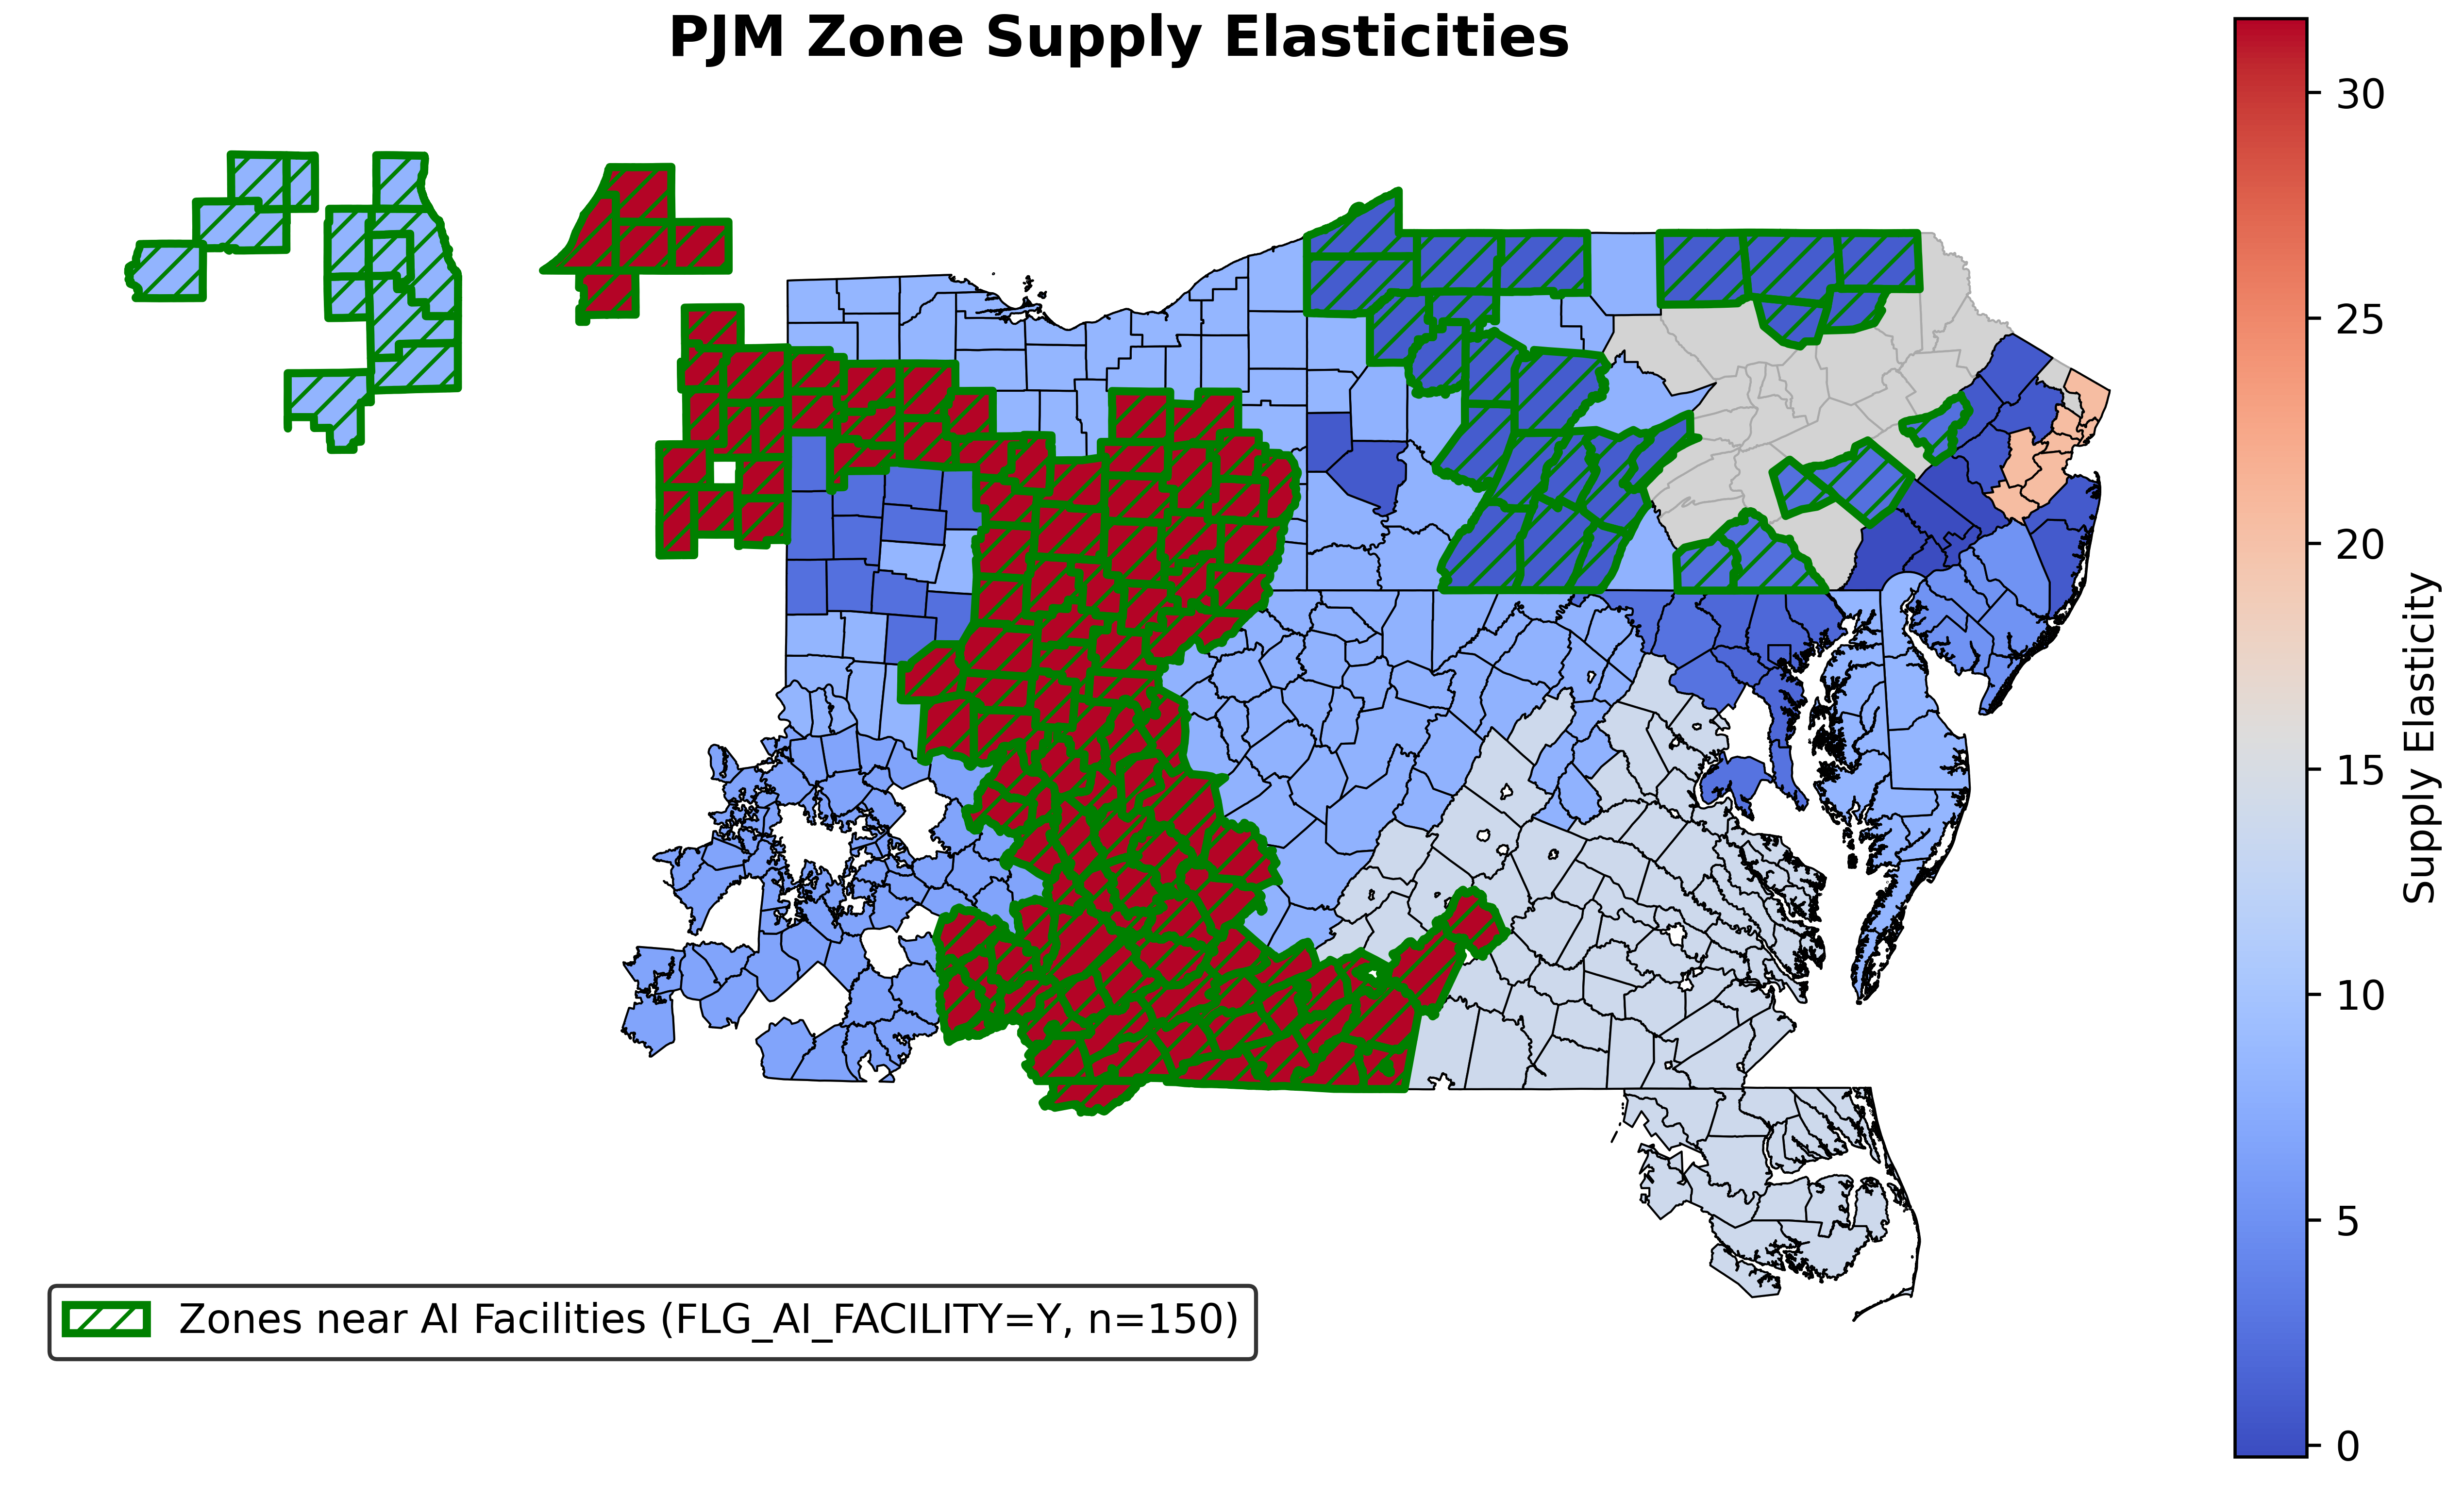
\includegraphics[width=0.5\linewidth]{Figures/pjm_ai_supply Elasticities.png}
    \caption{PJM Price Elasticity by Zone}
    \label{PJMPRiceElasticity}
\end{figure}

\subsection{Differences Between Power Quality and Demand Analyses}
\label{subsec:differences}

The power quality and fossil fuel demand analyses differ in geographic resolution and data structure due to the underlying data sources:

\begin{table}[t]
\centering
\resizebox{\columnwidth}{!}{%
\begin{tabular}{lcc}
\toprule
 & \textbf{Power Quality} & \textbf{Fossil Fuel Demand} \\
\midrule
Unit of observation & Utility-month & Generator-month \\
Geographic resolution & Utility service territory & Generator location \\
Treatment linkage & Utility contains AI data center & Generator near AI data center \\
Outcome source & Whisker Labs & EPA CEMS \\
Price endogeneity & Not modeled & IV with heat rate, gas price \\
\bottomrule
\end{tabular}
}
\caption{Summary of empirical designs}
\end{table}

These differences arise from data availability rather than conceptual distinctions. The power quality measures from Whisker Labs are aggregated to utility service territories, precluding finer spatial analysis. Generator-level EPA data permit more granular geographic matching, which we exploit for robustness analysis. The demand analysis additionally requires addressing price endogeneity because generation quantities reflect equilibrium outcomes in electricity markets; power quality indices are not directly determined by market clearing and thus do not require the same instrumentation strategy.

Despite these differences, we maintain a unified stacked DiD framework centered on model release dates for both analyses. This consistency facilitates comparison of effect dynamics across outcomes and provides a coherent narrative linking AI development activity to grid impacts.

\subsection{Additional Counterfactual Analysis}\label{Appendix:Counterfactuals}

\subsubsection{Training versus Inference Composition}

\textbf{Training-Inference Composition.} Third, we explore alternative compositions of AI workloads by selectively restricting channels in our model. By suppressing the training channel, we simulate power quality impacts under a scenario in which large-scale model training plateaus and the industry shifts toward an inference-dominant paradigm. Conversely, by suppressing the inference channel, we characterize outcomes under a shift toward primarily local, low-cost inference with reduced centralized training activity.

We explore how grid impacts would differ under alternative compositions of AI workloads.

\paragraph{Scenario: Inference-Dominant World.} If large-scale model training plateaus---perhaps due to diminishing returns to scale or compute constraints---while inference continues to grow with adoption, grid impacts would reflect primarily the inference channel.

\paragraph{Scenario: Training-Dominant World.} Conversely, if inference becomes predominantly local (on-device) while cloud resources are devoted primarily to training new models, impacts would concentrate in the training channel. Suppressing inference effects reduces additional power demand per hour per data center by significantly more than suppression of training. Figure~\ref{fig:channel_shutdown} provides insight into this relationship.

\begin{figure}[h]
    \centering
    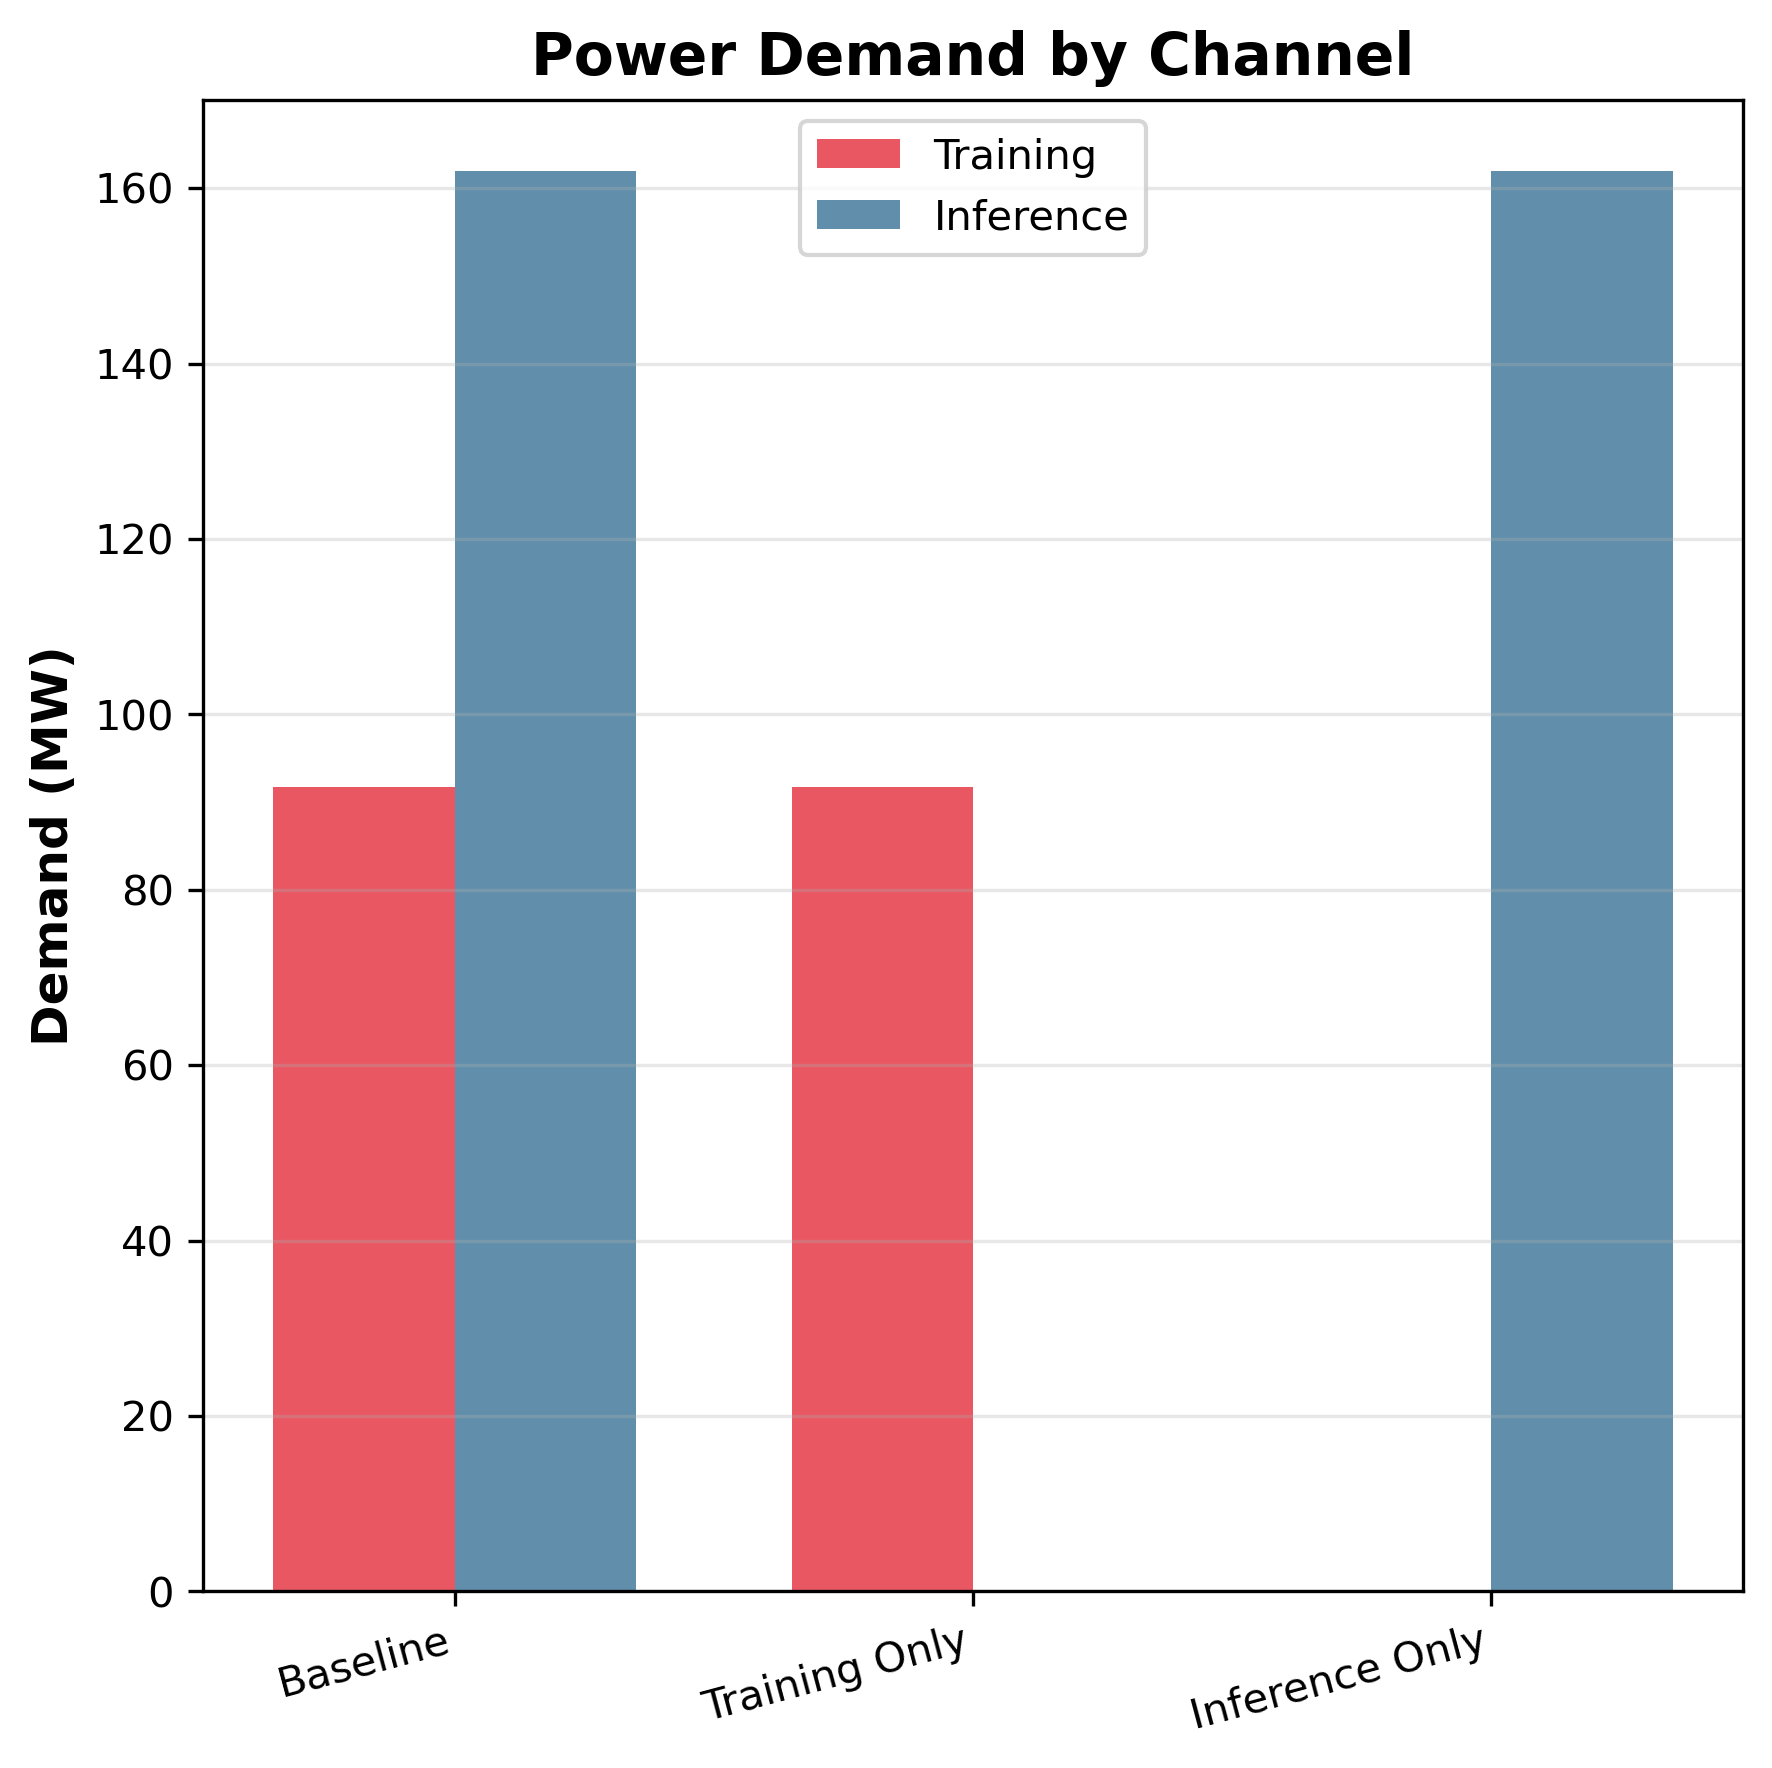
\includegraphics[width=0.5\linewidth]{Figures/channel_shutdown_analysis.png}
    \caption{Grid impacts under inference-only versus training-only scenarios.}
    \label{fig:channel_shutdown}
\end{figure}

\subsubsection{Efficiency Improvements}

\paragraph{Scenario: AI Efficiency Improvements.} Algorithmic efficiency represents a key lever for mitigating grid impacts. We calculate the potential impacts of efficiency gains, remaining agnostic about their source---improvements could come from both hardware and software advances related to AI training and inference. Figure~\ref{fig:efficiency_improvements} demonstrates how specific percentage-wise improvements in efficiency would affect the hourly demand coefficient. While a 40\% improvement in inference efficiency in our sample would lead to a 25\% reduction in total added demand, the same improvement in training efficiency would lead to only a 14\% reduction in demand.

\begin{figure}[h]
    \centering
    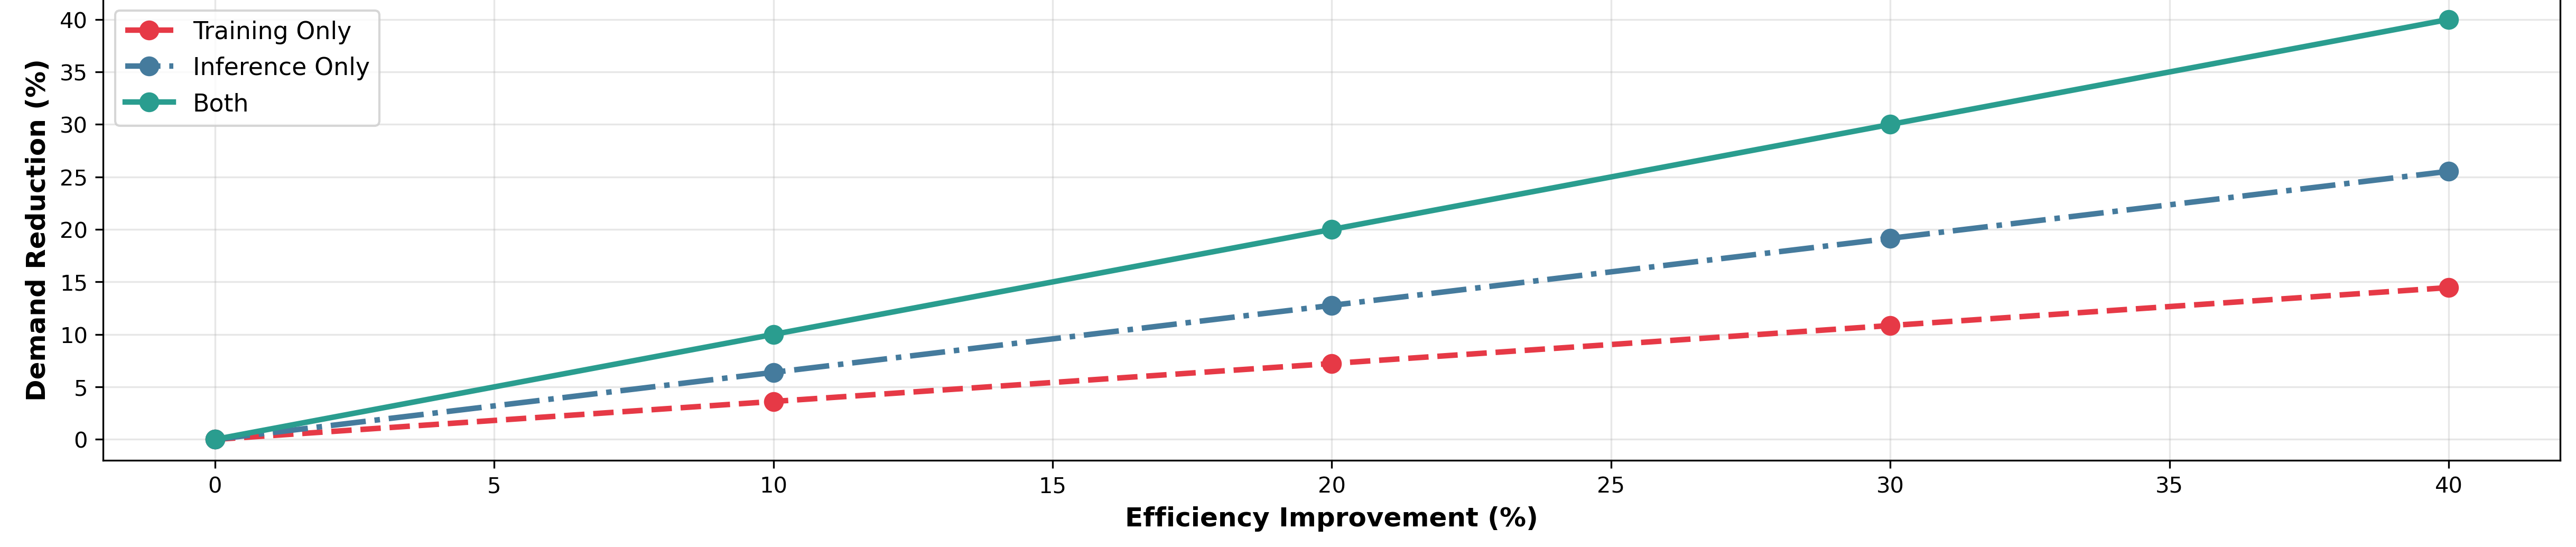
\includegraphics[width=0.5\linewidth]{Figures/comprehensive_counterfactual_summary.png}
    \caption{Reduction in power demand with efficiency improvements in training and inference.}
    \label{fig:efficiency_improvements}
\end{figure}

\subsubsection{Impacts of Agglomeration on Cost of System Outage}

\textbf{Impacts of Agglomeration on Cost of System Outage.} We examine the potential costs of agglomeration for cloud operators in terms of loss of service due to power outage. The concentration of AI workloads and AI data centers increases the strain in specific areas leading to greater costs on local grids and increasing the potential for long outages, which could lead to loss of service for cloud providers, which creates a significant revenue and reputational cost. These costs are bourne by data center operators themselves and so provide a non-socialized cost of data center impact on power grids that may justify spatial reorganization by the data center industry. We use publicly available estimates of the cost of recent losses of service by cloud platforms to tech companies to estimate these costs. 

Geographic concentration poses risks not only to the overall grid but also to cloud service reliability. The increased possibility of reliability events creates potential issues for cloud uptime and threatens continuous assurance of cloud services. As recently as 2022, a power failure in Ohio led to 3 continuous hours of downtime for Amazon Web Services US-EAST-2 \citep{Eisenberg2025AWSOutage}. Cloud losses were also associated with the blackouts during winter storm Uri in Texas. These outages impose costs on society as well as on hyperscalers in terms of lost revenue, damaged reputations, and security concerns.

We utilize documented estimates of outage costs from the literature (see Table~\ref{tab:outages} in Appendix Subsection ~\ref{app:outage_costs}) to estimate the economic costs to hyperscalers of increased reliability risk associated with data center concentration. We multiply the increase in the likelihood of a reliability event by the documented cost associated with a cloud outage of the length of a reliability event. We find that a shift to an edge-computing scenario as detailed above would lead to significant reliability-related savings for hyperscalers in our sample based only on treated models. Similarly, a full implementation of on-site colocated generation would lead to a total average decrease in the number of reliability events in data center utility areas of approximately .17 per month. This means that the number of reliability events per year making the IID assumption decreases by 2.04 events per year. We assume that a significant power outage that leads to a cloud outage has a median duration of 21 hours matching our data with a median cost per hour of 19.2 million. We further conservatively assume that a significant reliability event near a data center has a probability of leading to a cloud outage of 5\%. The implied reliability savings associated with on-site generation are thus \textbf{41 million} accrued to the hyperscaler. This is a significant financial argument for hyperscalers to work towards improved reliability.

\subsection{Treatment Definition and Data Linkage}
\label{subsec:treatment}

Our treatment relies on linking AI model releases to geographic regions through a chain of observable connections: models to companies, companies to data center locations, and data center locations to electricity service territories. We describe each link and its limitations.

\subsubsection{Identifying AI Data Centers}

We leverage a recently released variable from Aterio that directly classifies data centers by their primary use case, including a designation for AI-focused facilities. This classification improves upon prior approaches that treated all data centers homogeneously, as AI workloads---particularly large-scale model training---exhibit distinct load profiles characterized by sustained high utilization and substantial power draws that differ markedly from traditional cloud computing or storage operations.

We link data centers to electricity service territories at two geographic resolutions:
\begin{itemize}
    \item \textbf{Utility service territory:} For power quality analysis, we match AI data centers to retail electric utility boundaries. A utility is designated as treated if at least one AI data center operates within its service territory.
    \item \textbf{Generator proximity:} For fossil fuel demand analysis, we match data centers to generators by picking generators within a 20-mile radius of an in-sample data center. This finer resolution exploits the greater spatial granularity of EPA generator-level data.
\end{itemize}

\subsubsection{Linking Models to Data Centers}

We construct a crosswalk from AI model releases to data center locations through company ownership. For each major model release in our sample, we identify the developing company and link to all AI-classified data centers operated by or contracted to that company. 

\paragraph{Identifying Assumption and Limitations.} Our approach assumes that training and inference activity for a given model occurs at data centers associated with the releasing company. This assumption is imperfect for several reasons:
\begin{enumerate}
    % \item We do not observe the specific facility where training occurred. A company with multiple data centers may concentrate training at a subset of locations.
    \item Training may occur at third-party cloud facilities not captured in our data center inventory.
    \item Inference workloads may be distributed across facilities differently than training workloads.
\end{enumerate}

We interpret our estimates as capturing the \textit{average} effect across a company's AI data center footprint, which represents a lower bound on the localized effect at the actual training site if activity is concentrated, or an upper bound if we misattribute activity to facilities that were not involved. We probe robustness to this measurement error through several approaches described in Section~\ref{subsec:robustness}.

For a subset of models where public information permits more precise dating, we supplement our treatment timing with verified training and inference windows:

\subsection{Quantifying Costs of Loss of Cloud Services}\label{app:outage_costs}

Table~\ref{tab:outages} presents cloud service outages filtered to include only (1) incidents related to power infrastructure failures, or (2) incidents with verified financial impact estimates from cited sources. This dataset supports analysis of agglomeration costs for cloud operators arising from power grid strain and service disruption.

\begin{table}[t]
\centering
\scriptsize
\caption{Cloud Outages: Power-Related and Documented Costs (2021--2024)}\label{tab:outages}
\begin{tabular}{@{}lccrc@{}}
\toprule
Provider & HS & Pwr & Hrs & Cost \\
\midrule
% ERCOT~\cite{lee2022texas} & 0 & 1 & 71 & \$130B\textsuperscript{a} \\
OVHcloud~\cite{uptime2021ovh} & 0 & 1 & 288 & \euro10M\textsuperscript{b} \\
Fastly~\cite{fastly2021postmortem} & 0 & 0 & 1 & \$34M\textsuperscript{c} \\
GCP~\cite{dcd2022gcplondon} & 1 & 1 & 18 & --- \\
AWS~\cite{aws2022useast2} & 1 & 1 & 3 & --- \\
GCP~\cite{dck2022gcpiowa} & 1 & 1 & 4 & --- \\
Rackspace~\cite{rackspace2023sec} & 0 & 0 & 504 & \$35M\textsuperscript{d} \\
Alibaba~\cite{scmp2022alibaba} & 0 & 1 & 24 & --- \\
GCP~\cite{register2023gcpparis} & 1 & 1 & 336 & --- \\
CrowdStrike\textsuperscript{e}~\cite{parametrix2024crowdstrike} & 0 & 0 & 72 & \$5.4B\textsuperscript{f} \\
Alibaba~\cite{dcd2024alibabafire} & 0 & 1 & 144 & --- \\
GCP~\cite{register2024gcpfrankfurt} & 1 & 1 & 13 & --- \\
Azure~\cite{statusgator2024azure} & 1 & 1 & 6 & --- \\
\bottomrule
\end{tabular}

\vspace{0.3em}
\raggedright
\tiny
\textit{Notes:} HS = Hyperscaler (AWS/Azure/GCP). Pwr = Power/electrical/cooling/fire. Hrs = Duration.
\textsuperscript{a}TX total; \$4.3B direct.
\textsuperscript{b}Lawsuit awards.
\textsuperscript{c}Amazon only.
\textsuperscript{d}Revenue + remediation.
\textsuperscript{e}Third-party; affected Azure.
\textsuperscript{f}Fortune 500; insured \$0.5--1.1B.
\end{table}

\vspace{1em}
\noindent\textbf{Notes:}
\begin{enumerate}
    % \item[a.] Total economic impact estimate for Texas; \$4.3B in direct power costs per Dallas Fed.
    \item[b.] Lawsuit settlements; individual awards ranged \euro100K--\euro154K.
    \item[c.] Estimated Amazon revenue loss alone during 1-hour outage.
    \item[d.] Combines \$30M annual Hosted Exchange revenue loss plus \$5M remediation costs per SEC filings.
    \item[e.] Third-party vendor incident primarily affecting Microsoft Azure customers.
    \item[f.] Fortune 500 companies only; insured losses estimated \$540M--\$1.08B by Parametrix.
\end{enumerate}

\vspace{1em}
\noindent\textbf{Variable Definitions:}
\begin{itemize}
    \item \textbf{Hyperscaler}: Binary indicator (1 = AWS, Azure, or GCP; 0 = other providers).
    \item \textbf{Power}: Binary indicator (1 = outage caused by or related to power infrastructure, electrical systems, cooling failures, or fires; 0 = software, network, or security causes).
    \item \textbf{Duration}: Hours from incident onset to service restoration; ``+'' indicates ongoing recovery beyond initial resolution.
\end{itemize}

\subsubsection{Instrumental Variables Specification}\label{IVDetails}

The learned DiD coefficients capture the relationship between AI model releases and generator output, but this relationship may be confounded by supply-side shocks. For example, if AI model releases coincide with changes in natural gas prices or generator availability that independently affect electricity production, our estimates would conflate demand-side and supply-side effects. To isolate the demand-side effects, we instrument for electricity prices using the interaction of generator-level heat rates and regional natural gas prices. This instrumentation strategy exploits cross-sectional variation in generators' fuel efficiency: conditional on natural gas price movements, generators with higher heat rates (lower efficiency) face larger marginal cost shocks, allowing us to trace out the demand curve.

\paragraph{First-Stage and Structural Estimates.} The first stage regresses electricity prices on the heat rate--gas price interaction. The structural equation then uses predicted prices to estimate price responsiveness. The estimated price elasticity from the structural equation is 0.135 (SE = 0.013, p < 0.0001), indicating economically meaningful and precisely estimated demand responsiveness. As a specification check, we estimate the first stage separately for each of 5 model-specific regressions; the mean price coefficient is $-0.331$ (SD = 0.005, range: $-0.336$ to $-0.323$). The tight clustering of estimates across specifications suggests stable demand elasticity across AI model events and supports the validity of our instrumentation strategy.

\subsubsection{Interpretation and Caveats for Price Analysis}\label{appendix:Caveats}

These calculations provide ballpark estimates of how AI-induced demand shifts translate to wholesale price changes. Several caveats apply:
\begin{enumerate}
    \item The supply elasticity varies across regions and time periods; our estimates represent averages that mask considerable heterogeneity.
    \item If AI workloads can be temporally shifted to off-peak hours when supply is more elastic, price impacts would be smaller than our estimates suggest.
    \item We do not model transmission constraints, which may amplify local price effects in congested areas near data centers.
\end{enumerate}

\subsection{Wholesale-to-retail Passthrough Estimates}\label{WholesaleRetailPassthrough}

\begin{table}[H]
\centering
\caption{Wholesale-to-Retail Price Pass-Through in Deregulated Markets}
\label{tab:passthrough}
\scriptsize
\begin{tabular}{@{}llcc@{}}
\toprule
\textbf{Study} & \textbf{ISO} & \textbf{PT} & \textbf{Class} \\
\midrule
\multicolumn{4}{@{}l}{\textit{Panel A: Wholesale $\to$ Retail Pass-Through}} \\
\addlinespace[0.3em]
\citet{defeuilley2023pennsylvania} & PJM (PA) & 0.53 & Res. (EDC) \\
\citet{defeuilley2023pennsylvania} & PJM (PA) & 0.56 & Res. (EGS) \\
% \citet{tsai2025ohio} & PJM (OH) & ---$^a$ & Res. \\
\citet{brown2020texas} & ERCOT & 0.43--0.47 & Res. \\
\citet{mackay2024wholesale} & Multi & $\approx$1.0$^b$ & All \\
\midrule
\multicolumn{4}{@{}l}{\textit{Panel B: Demand Elasticity (Residential)}} \\
\addlinespace[0.3em]
\citet{deryugina2020longrun} & PJM (IL) & $-0.09$ & SR (1 mo.) \\
\citet{deryugina2020longrun} & PJM (IL) & $-0.27$ & MR (2 yr.) \\
\citet{deryugina2020longrun} & PJM (IL) & $-0.35$ & LR (10 yr.) \\
\bottomrule
\end{tabular}

\vspace{0.3em}
\raggedright
\scriptsize
\textit{Notes:} PT = pass-through coefficient. EDC = Electric Distribution Company; EGS = Electric Generation Supplier. SR/MR/LR = short/medium/long-run. \\
% $^a$Complex mechanism; volatility inflates auction premia. \\
$^b$Long-run; \$9.59/MWh cost $\to$ \$8.81/MWh retail.
\end{table}

\subsubsection{On-site Generation Estimation Details}
% \nb{move to appendix}
Data centers increasingly deploy on-site generation to reduce grid dependence. Our data center inventory identifies 87 facilities with on-site power generation capability and 12,401 without. We test whether on-site capacity moderates estimated effects by interacting treatment with on-site status in the utility-level strict DiD specification. Results indicate that on-site generation substantially mitigates measured grid impacts.

\begin{table}[h]
\centering
\caption{Power Quality Effects by On-site Generation Status}
\label{tab:btm_effects}
\resizebox{\columnwidth}{!}{% % This scales the table to fit
\begin{tabular}{lcccc}
\toprule
Outcome & With On-site & W/O On-site & Diff. & Interpretation \\
\midrule
CPQI & $-0.122$ & $+0.228$ & $-0.350$ & On-site reduces grid stress \\
% THD & $+0.120$ & $-2.174$ & $+2.294$ & BTM reduces harmonic distortion \\
\bottomrule
\end{tabular}%
}
\begin{flushleft}
\footnotesize\textit{Notes:} All coefficients significant at $p < 0.001$. CPQI: Consumer Power Quality Index.
\end{flushleft}
\end{table}

The sign reversal for CPQI is notable: data centers \textit{with} on-site generation are associated with improved power quality (negative coefficient), while those \textit{without} on-site generation are associated with deterioration (positive coefficient). This heterogeneity suggests that on-site generation absorbs demand spikes that would otherwise propagate to the grid, and implies that aggregate grid impacts understate total AI energy consumption. It should be noted that all large AI data centers in our most conservative sample had on-site generation. This may imply that our estimates of the impacts of on-site generation are exaggerated by a differential sample.

%\nb{Dana, why dont have we the parallel trends validation for power quality as well?}


\subsection{Additional Robustness Checks}\label{App:AdditionalRobustnessChecks}

% \subsubsection{Anomaly detection}

\subsubsection{Robustness Checks}
We test result robustness by varying treated population definitions, estimating specifications with alternative geographic boundaries to confirm consistency. This demonstrates findings reflect genuine causal impacts rather than arbitrary boundary choices. While we lack data on which models run at specific centers, our DiD methodology accounts for this by using publication dates as exogenous treatment, utilizing minimal geographic and temporal treatment windows. We plan robustness checks restricting treatment to larger data centers most likely involved in AI training. To verify treatment effects aren't noise-related, we include appendix robustness checks with randomized treatment dates as additional evidence that effects relate to model releases.

\subsubsection{Treatment Intensity}

Rather than binary treatment indicators, we estimate a continuous treatment intensity specification using total electricity demand (MWh) as the treatment variable. The significant coefficient (p < 0.001; THD: $+0.00018$, p < 0.001) indicate dose-response relationships: larger electricity loads are associated with larger power quality changes.

\subsubsection{Confirmed Locations and Verified Dates}

We re-estimate our main specifications using stricter treatment definitions. The confirmed-location analysis restricts treatment to facilities with precisely geocoded training locations (mean effect: 74.19 MWh). The verified-date analysis uses API release timing rather than publication dates from the Epoch database (mean effect: 63.20 MWh). Both analyses corroborate our main findings with expected attenuation from the more conservative treatment definitions.



\end{document}


% --- Restore bibliography commands ---
\let\bibliographystyle\origbibliographystyle
\let\bibliography\origbibliography
\let\wrapfigure\origwrapfigure
\let\endwrapfigure\origendwrapfigure

% --- Restore CAS affiliation ---
\let\affiliation\origaffiliation

\endgroup

% --- Per-chapter bibliography ---
\singlespacing
\bibliographystyle{plainnat}
\bibliography{Energy}
\doublespacing


\end{document}
